% ─────────────────────────────────────────────────────────────────────
% TWIN-LOCATION NOTICE. This file is one of the shared homes for the same
% results; edit every listed home or the drift checker fails.
%   Standalone paper : docs/harbor-research/tex/paper2.tex (S5 the theorem)
%   Chapter          : book/single-writer-kernel.tex (this file;
%                       "Synchronous guard sufficiency")
%   Index ids        : R5
%   Check            : python3 scripts/harbor-research/check_library_index.py
%                       python3 scripts/harbor-research/check_propagated_corrections.py
%                       python3 scripts/harbor-research/check_citations.py
%   System document  : docs/harbor-research/LIBRARY-SYSTEM.md
% ─────────────────────────────────────────────────────────────────────
\documentclass[11pt,a4paper]{article}

% ─── Packages ────────────────────────────────────────────────────────────────
\usepackage[utf8]{inputenc}
\usepackage[T1]{fontenc}
\usepackage{lmodern}
\usepackage{microtype}
\usepackage{geometry}
\usepackage{amsmath,amssymb,amsthm}
\usepackage{listings}
\usepackage{xcolor}
\usepackage{booktabs}
\usepackage{tabularx}
\usepackage{graphicx}
\usepackage{fancyhdr}
\usepackage{tikz}
\usepackage{pgfplots}
\pgfplotsset{compat=1.18}
\usetikzlibrary{arrows.meta,positioning,fit,backgrounds,calc,shapes.geometric,shapes.symbols,decorations.pathmorphing,decorations.pathreplacing}
\usepackage{float}
\usepackage{caption}
\usepackage{enumitem}
\usepackage[backref=page]{hyperref}
\captionsetup{font=small,labelfont=bf}
% Algorithms are formatted using lstlisting with custom pseudocode style

% ─── Geometry ────────────────────────────────────────────────────────────────
\geometry{margin=2.5cm}

% ─── Colors ──────────────────────────────────────────────────────────────────
\definecolor{codebg}{RGB}{248,248,248}
\definecolor{codeframe}{RGB}{200,200,200}
\definecolor{hhsand}{HTML}{E9DCC4}
\definecolor{hhsanddeep}{HTML}{D8C7A6}
\definecolor{hhebony}{HTML}{121212}
\definecolor{hhink}{HTML}{1B1712}
\definecolor{hhcobalt}{HTML}{003FB8}
\definecolor{hhamber}{HTML}{6B4500}
\definecolor{hhteal}{HTML}{00564C}
\definecolor{hhpaper}{HTML}{FBF7EF}
\definecolor{hhgray}{HTML}{5C5650}
% The Book's semantic color system: palette v2, light values. One hue, one meaning.
% Source of record for every hex: website-v2/src/styles/tokens.semantic.css (light
% theme); website-v2/scripts/check-figure-palette.mjs fails the build if this file
% and the tokens disagree. Twin copy under book/figures/ (byte-identical).
%
% Separation: contrast says an ink is READABLE on the cream; it says nothing about
% whether two inks are TELLABLE APART, and until now only the first was checked.
% check-figure-palette-separation.mjs measures all 21 pairs in OKLab with protanopia
% and deuteranopia simulated. indigo and violet are re-stepped (deeper, on their own
% hues, both gaining contrast) because they were the pairs with room: cobalt/indigo
% was dE 9.1 and is 15.1; cobalt/violet collapsed to 4.8 under protanopia and is 8.6.
% Three pairs CANNOT be fixed -- teal/health, gold/health and teal/gold have ceilings
% of 12.2, 13.9 and 14.3 against a floor of 15, because sRGB has no chroma to spend
% on the 112-182 degree arc this dark. Only ONE of gold, health and teal may carry a
% series by colour alone; the others need a label, a gap, or a texture.
%
% Discipline: story colors are accents (rules, fills, marks, display text); body
% pages stay cream and ink. Amber is stripes, dots, and display only, never small
% text (3.71:1 on cream). Violet and gold are AA as text; use them at display size
% or on rules and fills. Line weights: 1px texture, 1.5px linework, 2px enclosure.
\definecolor{pdcobalt}{HTML}{003FB8}      % kernel / truth            --brand-primary
\definecolor{pdteal}{HTML}{006B5F}        % legibility                --brand-accent
\definecolor{pdhealth}{HTML}{1F7A4D}      % ready / coordinated       --story-health
\definecolor{pdindigo}{HTML}{312865}      % protocol / federation     --story-indigo
\definecolor{pdviolet}{HTML}{822586}      % identity / continuity     --story-violet
\definecolor{pdrust}{HTML}{7A4514}        % reputation / trust earned --story-rust
\definecolor{pdgold}{HTML}{666A00}        % economy / value           --story-gold
\definecolor{pdslate}{HTML}{384856}       % foundation / bedrock      --story-slate
\definecolor{pderror}{HTML}{BF2F2F}       % breach / correction       --status-error
\definecolor{pdamber}{HTML}{A66F00}       % warning (display only)    --status-warning
\definecolor{pdlime}{HTML}{CAD900}        % highlight fill, ink text  --chart-yellow
\definecolor{pdink}{HTML}{121212}         % ink                       --text-primary
\definecolor{pdinkmuted}{HTML}{403B34}    % links, secondary text     --text-secondary
\definecolor{pdcream}{HTML}{F2EEE6}       % page ground               --surface-base
\definecolor{pdcreamraised}{HTML}{F7F3EB} % panels                    --surface-raised
\definecolor{pdcreamstrong}{HTML}{E9E2D5} % inset wells               --surface-strong
% Print inks for the Swiss edition of the Book (SWISS-BRIEF, B); print only.
\definecolor{pdswissblue}{HTML}{001489}
\definecolor{pdswissviolet}{HTML}{582C83}
\definecolor{pdswissred}{HTML}{DA291C}
% And the maritime edition's fourth ink: antique gold, the trim of the engraved
% plates carried onto the page (opener rules, part-title ornament, fillets round
% framed matter). Flat stand-in for a metallic pass; print only.
\definecolor{pdmaritimegold}{HTML}{805A14}

\newcommand{\pdchapterprefix}{swk}% this chapter's key in book/textbook.json
% GENERATED FILE. Do not edit by hand.
% Source of record: book/textbook.json (chapter order, numbers, parts, edition).
% Regenerate canonical map and site data: node scripts/generate-mega-whitepaper.mjs --sync-shared
% Drift check (CI): node --test scripts/generate-mega-whitepaper.test.mjs
% Canonical map: book/figures/pd-textbook-map.tex.
%
% Every standalone chapter preamble defines \pdchapterprefix before inputting
% this file; the Book redefines it at every \pdchapter. Everything else derives.

\providecommand{\pdeditiontitle}{Governing AI Agents: The Harbor, the Person, and the Economy}
\providecommand{\pdeditionsubtitle}{A Textbook of Concurrency, Identity, and Accountable Autonomous Work}
\providecommand{\pdeditionversion}{4.0 (Textbook Edition)}
\providecommand{\pdeditiondate}{5 November 2026}
\providecommand{\pdeditionclaim}{For autonomous work to remain accountable, each action needs an authority, a record, and someone responsible for its consequences.}
\providecommand{\pdbooktitle}{\emph{\pdeditiontitle}}
\providecommand{\pdchaptercount}{8}
\providecommand{\pdchaptercountword}{eight}
\providecommand{\pdpartcount}{4}
\providecommand{\pdchapterprefix}{none}
\expandafter\providecommand\csname pdchapternumberofnone\endcsname{0}
\expandafter\providecommand\csname pdchaptertitleofnone\endcsname{\pdeditiontitle}
\expandafter\providecommand\csname pdchaptercolorofnone\endcsname{pdcobalt}
\expandafter\providecommand\csname pdchapternumberofswk\endcsname{1}
\expandafter\providecommand\csname pdchaptertitleofswk\endcsname{The Single-Writer Kernel}
\expandafter\providecommand\csname pdchaptercolorofswk\endcsname{pdcobalt}
\expandafter\providecommand\csname pdchapterformerofswk\endcsname{II}
\expandafter\providecommand\csname pdchapterpartindexofswk\endcsname{1}
\expandafter\providecommand\csname pdchapterpartlabelofswk\endcsname{Part I \textperiodcentered\ Ground Truth}
\expandafter\providecommand\csname pdchapterquestionofswk\endcsname{Where can a rule be made real?}
\expandafter\providecommand\csname pdchapteronelineofswk\endcsname{A single program makes every change to a local database, one at a time; the chapter states which failures that record survives.}
\expandafter\providecommand\csname pdchapterepigraphofswk\endcsname{A transaction commits at the instant its commit record appears on disk.}
\expandafter\providecommand\csname pdchapterepigraphsourceofswk\endcsname{Jim Gray et al., The Recovery Manager of the System R Database Manager, 1981, p. 232}
\expandafter\providecommand\csname pdchapternumberofanchor\endcsname{2}
\expandafter\providecommand\csname pdchaptertitleofanchor\endcsname{The Anchor Protocol}
\expandafter\providecommand\csname pdchaptercolorofanchor\endcsname{pdcobalt}
\expandafter\providecommand\csname pdchapterformerofanchor\endcsname{V}
\expandafter\providecommand\csname pdchapterpartindexofanchor\endcsname{1}
\expandafter\providecommand\csname pdchapterpartlabelofanchor\endcsname{Part I \textperiodcentered\ Ground Truth}
\expandafter\providecommand\csname pdchapterquestionofanchor\endcsname{How may authority travel without silently growing?}
\expandafter\providecommand\csname pdchapteronelineofanchor\endcsname{When an agent passes a permission on, the new permission can only be narrower than the one it came from, at every step, and the checker verifies the whole chain.}
\expandafter\providecommand\csname pdchapterepigraphofanchor\endcsname{Every program and every user of the system should operate using the least set of privileges necessary to complete the job.}
\expandafter\providecommand\csname pdchapterepigraphsourceofanchor\endcsname{Jerome Saltzer and Michael Schroeder, The Protection of Information in Computer Systems, 1975}
\expandafter\providecommand\csname pdchapternumberofsealed\endcsname{3}
\expandafter\providecommand\csname pdchaptertitleofsealed\endcsname{The Sealed Harbor}
\expandafter\providecommand\csname pdchaptercolorofsealed\endcsname{pdcobalt}
\expandafter\providecommand\csname pdchapterformerofsealed\endcsname{}
\expandafter\providecommand\csname pdchapterpartindexofsealed\endcsname{1}
\expandafter\providecommand\csname pdchapterpartlabelofsealed\endcsname{Part I \textperiodcentered\ Ground Truth}
\expandafter\providecommand\csname pdchapterquestionofsealed\endcsname{What can a sealed agent leak, and how would we know?}
\expandafter\providecommand\csname pdchapteronelineofsealed\endcsname{A job run in a sealed environment can release results only through named checks, and all its releases together may disclose only a fixed amount of information, under the model's stated assumptions about channels.}
\expandafter\providecommand\csname pdchapterepigraphofsealed\endcsname{This note explores the problem of confining a program during its execution so that it cannot transmit information to any other program except its caller.}
\expandafter\providecommand\csname pdchapterepigraphsourceofsealed\endcsname{Butler W. Lampson, A Note on the Confinement Problem, 1973}
\expandafter\providecommand\csname pdchapternumberofls\endcsname{4}
\expandafter\providecommand\csname pdchaptertitleofls\endcsname{The Legible Swarm}
\expandafter\providecommand\csname pdchaptercolorofls\endcsname{pdteal}
\expandafter\providecommand\csname pdchapterformerofls\endcsname{I}
\expandafter\providecommand\csname pdchapterpartindexofls\endcsname{2}
\expandafter\providecommand\csname pdchapterpartlabelofls\endcsname{Part II \textperiodcentered\ The Cost of Seeing}
\expandafter\providecommand\csname pdchapterquestionofls\endcsname{What must remain visible, and what does seeing cost?}
\expandafter\providecommand\csname pdchapteronelineofls\endcsname{Useful supervision needs summaries that keep what the operator must decide on and link back to evidence the operator can inspect.}
\expandafter\providecommand\csname pdchapterepigraphofls\endcsname{In an information-rich world, the wealth of information means a dearth of something else: a scarcity of whatever it is that information consumes. What information consumes is rather obvious: it consumes the attention of its recipients.}
\expandafter\providecommand\csname pdchapterepigraphsourceofls\endcsname{Herbert A. Simon, Designing Organizations for an Information-Rich World, 1971}
\expandafter\providecommand\csname pdchapternumberofstp\endcsname{5}
\expandafter\providecommand\csname pdchaptertitleofstp\endcsname{From Spawn to Person}
\expandafter\providecommand\csname pdchaptercolorofstp\endcsname{pdviolet}
\expandafter\providecommand\csname pdchapterformerofstp\endcsname{III}
\expandafter\providecommand\csname pdchapterpartindexofstp\endcsname{3}
\expandafter\providecommand\csname pdchapterpartlabelofstp\endcsname{Part III \textperiodcentered\ What Survives the Restart}
\expandafter\providecommand\csname pdchapterquestionofstp\endcsname{What remains long enough to owe anything?}
\expandafter\providecommand\csname pdchapteronelineofstp\endcsname{An AI worker process starts, does a job and exits. Continuity links each replacement process, through a checked succession record, to one continuing account in a shared ledger, which shows what the worker owes, what it may do, which of its results an independent checker confirmed and which earlier processes it descends from. Reputation is what that record of confirmed results is worth to the next buyer.}
\expandafter\providecommand\csname pdchapterepigraphofstp\endcsname{We are but whirlpools in a river of ever-flowing water. We are not stuff that abides, but patterns that perpetuate themselves.}
\expandafter\providecommand\csname pdchapterepigraphsourceofstp\endcsname{Norbert Wiener, The Human Use of Human Beings: Cybernetics and Society, revised edition, 1954}
\expandafter\providecommand\csname pdchapternumberofhe\endcsname{6}
\expandafter\providecommand\csname pdchaptertitleofhe\endcsname{The Harbor Economy}
\expandafter\providecommand\csname pdchaptercolorofhe\endcsname{pdgold}
\expandafter\providecommand\csname pdchapterformerofhe\endcsname{IV}
\expandafter\providecommand\csname pdchapterpartindexofhe\endcsname{4}
\expandafter\providecommand\csname pdchapterpartlabelofhe\endcsname{Part IV \textperiodcentered\ Trade Between Strangers}
\expandafter\providecommand\csname pdchapterquestionofhe\endcsname{What makes cooperation rational without making loss unbounded?}
\expandafter\providecommand\csname pdchapteronelineofhe\endcsname{Labor, rented assets and licensed skills carry different risks, but all of them settle through one shared ledger in which no transfer creates or destroys any unit of payment.}
\expandafter\providecommand\csname pdchapterepigraphofhe\endcsname{The main reason why it is profitable to establish a firm would seem to be that there is a cost of using the price mechanism.}
\expandafter\providecommand\csname pdchapterepigraphsourceofhe\endcsname{Ronald H. Coase, The Nature of the Firm, 1937}
\expandafter\providecommand\csname pdchapternumberofbonded\endcsname{7}
\expandafter\providecommand\csname pdchaptertitleofbonded\endcsname{The Bonded Commons}
\expandafter\providecommand\csname pdchaptercolorofbonded\endcsname{pdgold}
\expandafter\providecommand\csname pdchapterformerofbonded\endcsname{VI}
\expandafter\providecommand\csname pdchapterpartindexofbonded\endcsname{4}
\expandafter\providecommand\csname pdchapterpartlabelofbonded\endcsname{Part IV \textperiodcentered\ Trade Between Strangers}
\expandafter\providecommand\csname pdchapterquestionofbonded\endcsname{Who may decide, on what evidence, with what consequence?}
\expandafter\providecommand\csname pdchapteronelineofbonded\endcsname{Some doubt about an agent's work remains even after access checks. The chapter handles it with shared rules: providers post deposits (bonds), signed records show who did what, audits sample the results, and either side can appeal a verdict. A model checker confirms, on a bounded model, that the deposit ledger never creates or loses money.}
\expandafter\providecommand\csname pdchapterepigraphofbonded\endcsname{The power to constrain an adversary may depend on the power to bind oneself.}
\expandafter\providecommand\csname pdchapterepigraphsourceofbonded\endcsname{Thomas C. Schelling, The Strategy of Conflict, 1960}
\expandafter\providecommand\csname pdchapternumberoffh\endcsname{8}
\expandafter\providecommand\csname pdchaptertitleoffh\endcsname{The Federated Harbor}
\expandafter\providecommand\csname pdchaptercoloroffh\endcsname{pdgold}
\expandafter\providecommand\csname pdchapterformeroffh\endcsname{VII}
\expandafter\providecommand\csname pdchapterpartindexoffh\endcsname{4}
\expandafter\providecommand\csname pdchapterpartlabeloffh\endcsname{Part IV \textperiodcentered\ Trade Between Strangers}
\expandafter\providecommand\csname pdchapterquestionoffh\endcsname{What can cross a trust boundary without moving the authority itself?}
\expandafter\providecommand\csname pdchapteronelineoffh\endcsname{Machines run by owners who do not trust each other can pass each other signed records, but not the power to approve actions on each other's systems. The chapter works out which information can spread from machine to machine, which decisions still need one designated approver, and why the receiving machine must issue its own permission for its own resources instead of narrowing the sender's.}
\expandafter\providecommand\csname pdchapterepigraphoffh\endcsname{We reject: kings, presidents and voting. We believe in: rough consensus and running code.}
\expandafter\providecommand\csname pdchapterepigraphsourceoffh\endcsname{David D. Clark, A Cloudy Crystal Ball: Visions of the Future, 1992}
\providecommand{\pdchapternumber}{\csname pdchapternumberof\pdchapterprefix\endcsname}
\providecommand{\pdchaptertitle}{\csname pdchaptertitleof\pdchapterprefix\endcsname}
\providecommand{\pdchaptercolor}{\csname pdchaptercolorof\pdchapterprefix\endcsname}
\providecommand{\pdchapterpartindex}{\csname pdchapterpartindexof\pdchapterprefix\endcsname}
\providecommand{\pdchapterpartlabel}{\csname pdchapterpartlabelof\pdchapterprefix\endcsname}
\providecommand{\pdchapterquestion}{\csname pdchapterquestionof\pdchapterprefix\endcsname}
\providecommand{\pdchapteroneline}{\csname pdchapteronelineof\pdchapterprefix\endcsname}
\providecommand{\pdchapterepigraph}{\csname pdchapterepigraphof\pdchapterprefix\endcsname}
\providecommand{\pdchapterepigraphsource}{\csname pdchapterepigraphsourceof\pdchapterprefix\endcsname}

% Parts, for the weighted four-hue rule: numeral, hue, the label that ends the
% part (the next part, or the appendices), and the chapter count used as the
% weight until page references exist. \pdweightrule (Book preamble) consumes it.
\providecommand{\pdfirstpartnumeral}{I}
\providecommand{\pdweightsegmentslist}{%
  \pdweightsegment{I}{pdcobalt}{part:II}{3}%
  \pdweightsegment{II}{pdteal}{part:III}{1}%
  \pdweightsegment{III}{pdviolet}{part:IV}{1}%
  \pdweightsegment{IV}{pdgold}{book:appendices}{3}%
}
\expandafter\providecommand\csname pdpartindexofI\endcsname{1}
\expandafter\providecommand\csname pdpartindexofII\endcsname{2}
\expandafter\providecommand\csname pdpartindexofIII\endcsname{3}
\expandafter\providecommand\csname pdpartindexofIV\endcsname{4}
\expandafter\providecommand\csname pdparttitleofI\endcsname{Ground Truth}
\expandafter\providecommand\csname pdparttitleofII\endcsname{The Cost of Seeing}
\expandafter\providecommand\csname pdparttitleofIII\endcsname{What Survives the Restart}
\expandafter\providecommand\csname pdparttitleofIV\endcsname{Trade Between Strangers}

% Locator map: every part and chapter of the Book, the current chapter marked.
% \pdchaplink is provided by figures/pd-hyperlinks.tex (a live link inside the
% Book, plain text in a standalone chapter).
\providecommand{\pdmapchapter}[3]{%
  \ifnum#1=\pdchapternumber\relax
    \textbf{\pdchaplink{#2}{#1.~#3}}~\textnormal{(this chapter)}%
  \else
    \pdchaplink{#2}{#1.~#3}%
  \fi}
\providecommand{\pdtextbookmap}{%
  \begin{tabular}{@{}l@{\quad}p{\dimexpr\linewidth-12em\relax}@{}}
  \textsc{\textbf{Part I}}\ Ground Truth & \raggedright \pdmapchapter{1}{swk}{The Single-Writer Kernel} \textperiodcentered\ \pdmapchapter{2}{anchor}{The Anchor Protocol} \textperiodcentered\ \pdmapchapter{3}{sealed}{The Sealed Harbor}\tabularnewline[2pt]
  \textsc{\textbf{Part II}}\ The Cost of Seeing & \raggedright \pdmapchapter{4}{ls}{The Legible Swarm}\tabularnewline[2pt]
  \textsc{\textbf{Part III}}\ What Survives the Restart & \raggedright \pdmapchapter{5}{stp}{From Spawn to Person}\tabularnewline[2pt]
  \textsc{\textbf{Part IV}}\ Trade Between Strangers & \raggedright \pdmapchapter{6}{he}{The Harbor Economy} \textperiodcentered\ \pdmapchapter{7}{bonded}{The Bonded Commons} \textperiodcentered\ \pdmapchapter{8}{fh}{The Federated Harbor}\tabularnewline[2pt]
  \end{tabular}}

% Shared pedagogic apparatus for the Book and every standalone chapter: boxed
% claims, honest boundaries, worked examples, retrieval prompts, numbered
% exercises, and their deferred solutions.
% Twin copy under book/figures/ (byte-identical; checked by
% scripts/generate-mega-whitepaper.test.mjs).
%
% \input this immediately after figures/pd-textbook-map (so \pdchapterprefix
% and \pdchapternumber already resolve) and before figures/pd-hyperlinks.
%
% Page grammar (Wave 12): a content kind is signalled by typography and the
% margin, never by a tinted rectangle. Claims: a hairline above, a small-caps
% run-in head, a short hairline below. Worked examples: two hairlines and an
% italic head. Boundaries: a plain ink bar at the left, no fill. Recitation:
% margin prompts in the Book, a compact list in a standalone chapter.
% Exercises: a numbered hanging paragraph with kind and stars in small caps,
% the solution page in the margin. Nothing here paints a background.
%
% \ifpdmargincolumn is false by default (standalone A4 chapters have no margin
% column); the Book's preamble sets \pdmargincolumntrue after its geometry.
% mdframed is used only for the bars (leftline) and hairlines (top/bottom),
% with the DEFAULT frame method -- never framemethod=tikz.
%
% Key-value parsing for \pdexercise uses pgfkeys: pgf ships as part of tikz,
% which every preamble already loads, so this adds no new dependency (keyval
% would have meant one). The closed kind/rating vocabularies are enforced with
% the LaTeX kernel's own \in@/\ifin@ comma-list test -- always available,
% no package of its own -- wrapped in an \edef that expands both sides first:
% \in@ does not expand its own arguments, so hunting for a *macro* (rather
% than literal text) requires pre-expanding it, or every kind reads as absent.
\makeatletter
\@ifpackageloaded{mdframed}{}{\usepackage{mdframed}}
\@ifpackageloaded{answers}{}{\usepackage{answers}}
\@ifpackageloaded{marginnote}{}{\usepackage{marginnote}}
\@ifpackageloaded{environ}{}{\usepackage{environ}}
\@ifpackageloaded{etoolbox}{}{\usepackage{etoolbox}}
\@ifpackageloaded{listings}{}{\usepackage{listings}}
\@ifpackageloaded{caption}{}{\usepackage{caption}}
\@ifpackageloaded{tcolorbox}{}{\usepackage[skins,breakable,listings]{tcolorbox}}

% ---------------------------------------------------------------------------
% Shared helpers: the margin-column switch, the margin head, the margin glyph.
% ---------------------------------------------------------------------------
% The Book defines \pdcurrentchaptercolor (per part) AFTER this file; a
% standalone chapter never does. Resolve it lazily, falling back to cobalt.
\newcommand{\pd@chaptercolor}{\ifdefined\pdcurrentchaptercolor\pdcurrentchaptercolor\else pdcobalt\fi}
% The eight standalone chapter PDFs this false branch exists for are retired
% as of this change (the chapters no longer build or publish an A4 edition of
% themselves). Every \ifpdmargincolumn false branch below is now dead weight
% kept alive only by the chapters' .tex sources still being independently
% compilable; do NOT delete it in this change -- the margin apparatus work is
% in flight on another branch and this would collide with it. Removing the
% false branch (and, eventually, the conditional itself) is that wave's job.
\newif\ifpdmargincolumn
\pdmargincolumnfalse
% The Book overrides this with an unnumbered, baseline-aligned margin aside.
% Keep chapter sources independently compilable without duplicating prose.
\providecommand{\pdsourceaside}[1]{\footnote{#1}}
% An intentional body boundary: flush pending figures before a new margin
% discussion. The generator strips legacy literal chapter-opening breaks,
% but preserves this explicit editorial instruction. Never use it in frames.
\newcommand{\pdmarginpagebreak}{\clearpage}
\renewcommand*{\marginfont}{\footnotesize\raggedright\color{pdinkmuted}}
% A small-caps head: set in the margin when the Book has a margin column,
% otherwise run in at the start of the paragraph.
% A head stays a \marginnote, and the reason is worth keeping. It was set as
% a \marginpar for one build (2026-09-08), so the page builder would keep the
% Recall block clear of it, and the build died with "Float(s) lost" at the end
% of chapter 1. \ifinner is true inside a minipage or mdframed only BETWEEN
% paragraphs; the moment a paragraph starts it is ordinary horizontal mode,
% \ifinner is false, and a \marginpar issued there -- a \keyidea inside a
% pdexample -- has no page to be shipped to. The heads are one line each and
% are never what runs into something; the Recall block was, and it is now a
% \marginpar issued in vertical mode, where the test is honest.
% Each head records the page and the page-height at which it was issued, so a
% Recall block raised later on the same page can stop short of it. A head is
% issued at the start of its paragraph, where \pagetotal is the page above the
% paragraph -- the head's own position, to within a line.
% Margin occupancy is tracked both ways. A head records where it was issued
% so a Recall block raised later on the page stops short of it; a Recall block
% records where its foot came to rest so a head issued later on the same page
% (the next section's first Key idea) steps down below it instead of printing
% inside it. \pagetotal at a head lags by the current paragraph, which puts
% every error on the safe side: the block is capped a little low, the head
% steps a little far.
\def\pd@lastheadpage{0}\newlength{\pd@lastheadbottom}
\def\pd@blockpage{0}\newlength{\pd@blockbottom}\newlength{\pd@headshift}
\newsavebox{\pd@headbox}\newsavebox{\pd@ptrbox}\newsavebox{\pd@sidebox}
% Run the page builder so \pagetotal counts the paragraph that just ended.
% Without it \pagetotal is the page above the LAST paragraph the builder saw,
% which under-reads by however much prose has since been set -- and every
% device here decides where it may sit from that number. A Boundary head read
% a stale \pagetotal and recorded its foot a paragraph too high, and the Recall
% block that followed cleared that phantom and printed on the head itself
% (0.1 pt apart on p. 253 of the technical edition). \penalty\@M contributes
% without opening a breakpoint. Outer vertical mode only: inside a box the
% penalty lands on the box's own list and settles nothing.
\newcommand{\pd@settle}{\ifvmode\ifinner\else\penalty\@M\vskip\z@\fi\fi}
% ---------------------------------------------------------------------------
% Figure-band tracking, for vertical CENTERING of a margin device against the
% main-column figure it accompanies (2026-09). \pd@figtop/\pd@figbot/\pd@figpage
% are declared here but SET in the Book preamble's \pgfsys@typesetpicturebox
% hook (coordination-papers-mega-volume-preamble.tex), not by an
% \AtBeginEnvironment{figure}/\AtEndEnvironment{figure} pair on \pagetotal --
% that was the first attempt and it does not work: for a \begin{figure}[H]
% float, the `float' package defers inserting the box into the main vertical
% list past \end{figure} itself, so \pagetotal read there under-reads by the
% whole figure and \pd@figbot always came out equal to \pd@figtop (measured:
% every firing in the built Book). The pgf hook that already intercepts every
% TikZ picture on its way into the page knows the box's own \ht+\dp directly,
% which is exact regardless of page-builder timing, so that is where the span
% is recorded now. \pd@figpage guards against reading a stale span left over
% from a figure several pages back: \pd@placemargin only trusts the span when
% \pd@figpage still equals the numeric page counter. Only one span is kept -- the most
% recently drawn picture on this page -- which is deliberately the figure a
% margin device issued shortly afterward is almost always about; a page with
% two unrelated figures and one margin device between them is not a case this
% file has seen.
\newlength{\pd@figtop}\newlength{\pd@figbot}\def\pd@figpage{0}
% Does OFFSET (already sitting in \pd@blockoff) sit inside the room this page
% actually has for it, without moving? \pd@reqmin/\pd@reqmax are computed by
% \pd@marginbounds below, from exactly the three collision facts \pd@placemargin
% already knew about (page top, the last margin head, the last margin block) --
% this is a read of the same facts, not a new rule. A candidate that fits
% clean is preferred over one merely clamped INTO range, because a clamped
% value is a collision this page already had; a candidate the bounds do not
% touch is one that was never in anyone's way.
\newlength{\pd@reqmin}\newlength{\pd@reqmax}\newif\ifpd@havemax\newif\ifpd@fits
\newcommand{\pd@marginbounds}[1]{%
  \setlength{\pd@reqmin}{-\pagetotal}%
  \ifnum\pd@lastheadpage=\value{page}\relax
    \ifdim\pd@reqmin<\dimexpr\pd@lastheadbottom-\pagetotal\relax
      \setlength{\pd@reqmin}{\dimexpr\pd@lastheadbottom-\pagetotal\relax}\fi\fi
  \ifnum\pd@blockpage=\value{page}\relax
    \ifdim\pd@reqmin<\dimexpr\pd@blockbottom-\pagetotal+2pt\relax
      \setlength{\pd@reqmin}{\dimexpr\pd@blockbottom-\pagetotal+2pt\relax}\fi\fi
  \ifdim\pagegoal<\maxdimen
    \pd@havemaxtrue
    \setlength{\pd@reqmax}{\dimexpr\pagegoal-\pagetotal-\ht#1-\dp#1\relax}%
  \else\pd@havemaxfalse\fi}
\newcommand{\pd@tryoffset}{%
  \pd@fitstrue
  \ifdim\pd@blockoff<\pd@reqmin\pd@fitsfalse\fi
  \ifpd@fits\ifpd@havemax\ifdim\pd@blockoff>\pd@reqmax\pd@fitsfalse\fi\fi\fi}
\newcommand{\pd@marginhead}[1]{%
  \ifpdmargincolumn
    % Settle before the first \pagetotal read, unlike this macro's earlier
    % form. Every OTHER margin device in this file settles first (the
    % comment two macros up even says why: "\pagetotal is the page above
    % the LAST paragraph the builder saw"), but this one read \pagetotal
    % raw at the head's own issuing point and called the resulting slop
    % "to within a line" -- acceptable when a block follows a head closely,
    % not when many lines of prose come between them and a margin block
    % later clamps to \pd@lastheadbottom expecting it exact. Measured: a
    % \pdboundary head ("Where this stops") 14 lines above its section's
    % \end{pdrecitation}, recorded 2.35 pt short, so the Recall block's
    % clamp (aimed at a 3 pt gap under the head) landed 2.35 pt INSIDE it
    % instead -- built and measured overlapping, PDF p. 244.
    \pd@settle
    \setlength{\pd@headshift}{0pt}%
    \ifnum\pd@blockpage=\value{page}\relax
      \ifdim\pagetotal<\pd@blockbottom
        \setlength{\pd@headshift}{\dimexpr\pd@blockbottom-\pagetotal+3pt\relax}\fi
    \fi
    % And around the last HEAD on this page, which this macro recorded below
    % and then never read. Blocks stepped around heads, heads stepped around
    % blocks, and two heads walked straight through each other: a Pitfall head
    % printed 1.0 pt from a Recall head at the top of p. 306 of the maritime
    % edition, inside the 10.4 pt leading the collision check measures. The
    % rule is the same one \pd@placemargin already obeys three lines at a
    % time -- never above what is already in the column -- so it is applied
    % here in the same shape, after the block cap so whichever foot sits
    % lower wins.
    \ifnum\pd@lastheadpage=\value{page}\relax
      \ifdim\dimexpr\pagetotal+\pd@headshift\relax<\pd@lastheadbottom
        \setlength{\pd@headshift}{\dimexpr\pd@lastheadbottom-\pagetotal+3pt\relax}\fi
    \fi
    % A twin of the head, set at the margin's width and font, measured but
    % never shipped: a head of three or four words wraps to two lines there,
    % and a block raised later on the page has to clear the head's real foot.
    % Assuming one line put "RECALL" 0.1 pt under "WHERE THIS STOPS" in the
    % Swiss and technical editions, whose pagination differs from the
    % maritime edition's by a page.
    \sbox{\pd@headbox}{\begin{minipage}{\marginparwidth}\marginfont\scshape #1\end{minipage}}%
    \marginnote{\scshape #1}[\pd@headshift]%
    \xdef\pd@lastheadpage{\number\value{page}}%
    % +8pt, not +3pt: \pd@headbox measures the head's own text, but the
    % marginnote package sets every note's content behind a \strut (its
    % \marginfont\raggedrightmarginnote\strut...) whose height+depth come
    % from \marginfont's normal font metrics, not from \scshape "Where this
    % stops" alone -- the strut is measurably taller, so \ht+\dp here
    % under-reads the head's true rendered bottom. +3pt covered one 0.1pt
    % case (comment above); it did not cover this one -- built and measured
    % a Recall block clamped to +3pt still overlapping "Where this stops" by
    % 2.35 pt (PDF p. 244, pdboundary fourteen lines above its section's
    % \end{pdrecitation}). +8pt re-measured clear on that page and does not
    % reopen the "1.3 pt under" case the \newpage reservation above already
    % handles (a different mechanism -- a migrated page, not a short strut).
    \global\pd@lastheadbottom=\dimexpr\pagetotal+\pd@headshift
      +\ht\pd@headbox+\dp\pd@headbox+8pt\relax
  \else{\scshape #1.}\enspace\fi}
% A small square in the chapter's hue, in the margin, marking a worked example
% so a reader flipping through finds every one.
\newlength{\pd@blockoff}
% Place a measured margin block so its LAST line sits on the line that issues
% it -- the block occupies the page above its anchor rather than hanging below
% it, which is what keeps a note issued near the foot on the paper at all.
% Three caps, in order: never above the page top; never above the last margin
% head on this page (measured to that head's own foot); never above the last
% block on this page. Then the block records where its foot came to rest, so a
% head issued later steps down below it. \pagetotal is the shared clock for all
% of this, which is why every device that can settles the page builder first.
% Every margin device goes through here, including the three the margin
% apparatus added (\pdcite, \pdprov, \pdprovedon): a device that places its
% own note without asking what is already in the column is how the Book got
% seven collisions and a portrait below the paper, and there are now several
% hundred short notes in the column where there were dozens.
% Place a margin block with its TOP on the issuing line rather than its foot.
% Same occupancy bookkeeping as \pd@placemargin -- it must, or a later block
% would be told the column is free where this one sits -- but it never raises,
% so it cannot leave the page above. Clamped both ways: the offset is never
% negative (nothing above the text block) and, where \pagegoal is a real
% dimension, never so large that the block's foot passes the bottom of the
% text block. \pagegoal is \maxdimen on an empty page, which is room for
% anything; a block already taller than its page is left alone rather than
% shoved, because moving it cannot make it fit.
\newlength{\pd@blockfloor}
\newcommand{\pd@placemargintop}[1]{%
  \setlength{\pd@blockoff}{0pt}%
  \ifnum\pd@lastheadpage=\value{page}\relax
    \ifdim\pd@blockoff<\dimexpr\pd@lastheadbottom-\pagetotal\relax
      \setlength{\pd@blockoff}{\dimexpr\pd@lastheadbottom-\pagetotal\relax}\fi
  \fi
  \ifnum\pd@blockpage=\value{page}\relax
    \ifdim\pd@blockoff<\dimexpr\pd@blockbottom-\pagetotal+2pt\relax
      \setlength{\pd@blockoff}{\dimexpr\pd@blockbottom-\pagetotal+2pt\relax}\fi
  \fi
  \ifdim\pd@blockoff<0pt \setlength{\pd@blockoff}{0pt}\fi
  % The floor the two caps above just established: whatever is already in the
  % column on this page ends here, and nothing may be placed above it.
  \setlength{\pd@blockfloor}{\pd@blockoff}%
  % Pull the block up if its foot would pass the bottom of the text block --
  % but never above that floor. Reducing the offset past it is how the
  % foot-anchored placement used to undo its own downward pushes: a clamp
  % applied last re-collides the block with the head or the note it was just
  % moved clear of, which is the defect this file's other comment records as
  % 132 collisions on one merge. A block too tall to satisfy both is left at
  % the floor and overruns the foot, where page_overflow.py's foot-intrusion
  % and off-the-paper checks will report it -- a visible, measured overrun is
  % worth more than a silent overlap.
  \ifdim\pagegoal<\maxdimen
    \ifdim\dimexpr\pagetotal+\pd@blockoff+\ht#1+\dp#1\relax>\pagegoal
      \setlength{\pd@blockoff}{\dimexpr\pagegoal-\pagetotal-\ht#1-\dp#1\relax}%
      \ifdim\pd@blockoff<\pd@blockfloor \setlength{\pd@blockoff}{\pd@blockfloor}\fi
    \fi
  \fi
  \marginnote{\usebox#1}[\pd@blockoff]%
  \xdef\pd@blockpage{\number\value{page}}%
  \global\pd@blockbottom=\dimexpr\pagetotal+\pd@blockoff+\ht#1+\dp#1\relax}

% Default placement is now CENTERED on the vertical span of the most recently
% closed figure on this page, not anchored to the line that issues the note --
% a Recall block or a gloss discussing a figure reads naturally beside its
% middle, not hanging off one edge. Center only WHEN IT FITS CLEAN: tried
% against \pd@marginbounds's read of the same three collision facts the old
% single anchor already obeyed (page top, the last margin head, the last
% margin block), with no clamping. A center that does not fit clean is not
% clamped into place -- clamping a center is neither center nor top nor
% bottom, it is just wherever the clamp landed, and the point of asking for an
% aligned center was to get one honestly or not at all. Top-of-figure is tried
% next, then bottom-of-figure; the first of the three that needs no clamp
% wins. If none does, this falls through unchanged to the pre-existing
% issuing-line anchor and its own clamps below -- the same fallback this file
% always had, now reached only when no figure-relative placement clears.
\newif\ifpd@figcentered
\newcommand{\pd@placemargin}[1]{%
  \pd@figcenteredfalse
  \ifnum\pd@figpage=\value{page}\relax\ifdim\pd@figbot>\z@
    \pd@marginbounds{#1}%
    \setlength{\pd@blockoff}{\dimexpr(\pd@figtop+\pd@figbot)/2-\pagetotal-(\ht#1+\dp#1)/2\relax}%
    \pd@tryoffset
    \ifpd@fits\pd@figcenteredtrue\else
      \setlength{\pd@blockoff}{\dimexpr\pd@figtop-\pagetotal\relax}%
      \pd@tryoffset
      \ifpd@fits\pd@figcenteredtrue\else
        \setlength{\pd@blockoff}{\dimexpr\pd@figbot-\pagetotal-\ht#1-\dp#1\relax}%
        \pd@tryoffset
        \ifpd@fits\pd@figcenteredtrue\fi
      \fi
    \fi
  \fi\fi
  \ifpd@figcentered
    \marginnote{\usebox#1}[\pd@blockoff]%
    \xdef\pd@blockpage{\number\value{page}}%
    \global\pd@blockbottom=\dimexpr\pagetotal+\pd@blockoff+\ht#1+\dp#1\relax
  \else
  \setlength{\pd@blockoff}{\dimexpr\baselineskip-\ht#1-\dp#1\relax}%
  % A note never starts below the line that issues it -- clamped here, BEFORE
  % the occupancy caps, not after. Clamping last undid every downward push:
  % two \pdcite calls in one paragraph read the same \pagetotal, so the second
  % was told to start below the first's foot and then clamped straight back
  % onto it (132 collisions on the merge, all of them pairs of citations on
  % one line). Below the anchor is exactly where a second note belongs.
  \ifdim\pd@blockoff>0pt \setlength{\pd@blockoff}{0pt}\fi
  \ifdim\pd@blockoff<-\pagetotal
    \setlength{\pd@blockoff}{-\pagetotal}%
    % Headroom at the column top, and the reason is the one hole left in the
    % occupancy model. Every cap below is keyed on the numeric page counter, which is the
    % page the device was ISSUED on -- and a head issued in the last line of
    % a page whose paragraph then breaks prints at the top of the NEXT page
    % while having recorded the page before. That is exactly the Recall-on-
    % Pitfall collision at the top of p. 306 of the maritime edition: the
    % Pitfall head began its paragraph at the foot of p. 305, migrated with
    % the break, and the Recall block clamped flush to p. 306's column top
    % and landed 1.0 pt from a head no cap could see. TeX cannot tell us the
    % shipout page here, so the fix is not a better cap but a reservation:
    % when the top clamp binds, leave two lines for whatever may have come
    % over the break. Two, not one, because a head of three or four words
    % wraps to two lines at the margin's width. Only when there is room --
    % \pagegoal is \maxdimen on an empty page, which is room enough for
    % anything, and a block already too tall for its page is left where the
    % clamp put it rather than pushed off the paper.
    \ifdim\dimexpr\pagetotal+\pd@blockoff+2\baselineskip+\ht#1+\dp#1\relax>\pagegoal
      \ifdim\dimexpr\pagetotal+\pd@blockoff+\baselineskip+\ht#1+\dp#1\relax>\pagegoal
      \else\setlength{\pd@blockoff}{\dimexpr\pd@blockoff+\baselineskip\relax}\fi
    \else\setlength{\pd@blockoff}{\dimexpr\pd@blockoff+2\baselineskip\relax}\fi
  \fi
  \ifnum\pd@lastheadpage=\value{page}\relax
    \ifdim\pd@blockoff<\dimexpr\pd@lastheadbottom-\pagetotal\relax
      \setlength{\pd@blockoff}{\dimexpr\pd@lastheadbottom-\pagetotal\relax}\fi
  \fi
  \ifnum\pd@blockpage=\value{page}\relax
    \ifdim\pd@blockoff<\dimexpr\pd@blockbottom-\pagetotal+2pt\relax
      \setlength{\pd@blockoff}{\dimexpr\pd@blockbottom-\pagetotal+2pt\relax}\fi
  \fi
  \marginnote{\usebox#1}[\pd@blockoff]%
  \xdef\pd@blockpage{\number\value{page}}%
  \global\pd@blockbottom=\dimexpr\pagetotal+\pd@blockoff+\ht#1+\dp#1\relax
  \fi}
% The same placement for a note the page can do without. A Recall block, a
% margin figure and a gloss carry content that is nowhere else, so they are
% always placed. A short-form citation, a provenance note and a discharge
% pointer are second copies: \pdcite has already emitted the \cite, so the
% work is in the text and in the bibliography whatever the margin does. There
% are several hundred of them and on a dense page the column has no room for
% one beside every line that cites -- arithmetic cannot make space that is not
% there. So when placing one would push its foot past the text block's foot,
% it is left out rather than printed over its neighbour or below the paper.
% Nothing is lost that a reader could otherwise have read.
\newcommand{\pd@placemarginopt}[1]{%
  \setlength{\pd@blockoff}{\dimexpr\baselineskip-\ht#1-\dp#1\relax}%
  \ifdim\pd@blockoff>0pt \setlength{\pd@blockoff}{0pt}\fi
  \ifdim\pd@blockoff<-\pagetotal \setlength{\pd@blockoff}{-\pagetotal}\fi
  \ifnum\pd@lastheadpage=\value{page}\relax
    \ifdim\pd@blockoff<\dimexpr\pd@lastheadbottom-\pagetotal\relax
      \setlength{\pd@blockoff}{\dimexpr\pd@lastheadbottom-\pagetotal\relax}\fi
  \fi
  \ifnum\pd@blockpage=\value{page}\relax
    \ifdim\pd@blockoff<\dimexpr\pd@blockbottom-\pagetotal+2pt\relax
      \setlength{\pd@blockoff}{\dimexpr\pd@blockbottom-\pagetotal+2pt\relax}\fi
  \fi
  % Room left on this page, measured to the block's foot, with two lines of
  % slack. \pagegoal is \maxdimen while the page is empty, which is room
  % enough for anything. The slack is there because \pagetotal under-reads
  % mid-paragraph, which is where most of these are called: without it the
  % guard believed there was room and put an Exercises pointer 8.2 pt off the
  % foot of p. 309 of the Swiss edition -- a page that only exists in the CI
  % build's pagination, which is why the local builds were clean and the check
  % running over every edition in CI is what found it.
  \ifdim\dimexpr\pagetotal+\pd@blockoff+\ht#1+\dp#1+2\baselineskip\relax>\pagegoal
  \else
    \marginnote{\usebox#1}[\pd@blockoff]%
    \xdef\pd@blockpage{\number\value{page}}%
    \global\pd@blockbottom=\dimexpr\pagetotal+\pd@blockoff+\ht#1+\dp#1\relax
  \fi}
\newcommand{\pd@marginglyph}{%
  \ifpdmargincolumn\marginnote{\textcolor{\pd@chaptercolor}{\rule[-0.5pt]{4.5pt}{4.5pt}}}\fi}

% \pdgloss{Term}{one-line definition} -- a defined term set bold where it is
% defined, in the running text, the way the Book already sets any term of art
% at its point of definition; the definition itself is carried as a margin
% note rather than left inline, so a reader can recall it from the margin
% without re-parsing the sentence. In the margin column (Book) this reuses
% the small-caps head convention \pd@marginhead sets for \keyidea, \pitfall
% and \xrefbox's own heads, but folds head and body into ONE \marginnote call
% -- calling \pd@marginhead and a separate \marginnote back to back would
% place two independent margin boxes at the same source line and risk them
% colliding, exactly what \pdmarginfigure avoids by building one combined box
% for its image and caption. The margin text renders at \marginfont, the
% same footnotesize sidenote size every other margin note in this file uses.
% Outside the margin column (standalone chapters) the definition folds back
% into the sentence as a parenthetical, so no content is lost. No box, no
% rule -- a bare labelled aside like every other device here. No trailing
% \ignorespaces: unlike \pdboundary/\pdexample (environments whose content
% starts on the next source line), \pdgloss is called mid-sentence and the
% genuine word space that follows it in the prose must survive.
% The note is measured and RAISED so its last line sits on the line that
% issues it, for the same reason the Recall block is: a gloss called in the
% last line or two of a page hung its definition below the paper, where the
% log says nothing and the reader has nothing (Lamport's gloss, 81 pt off the
% foot of p. 68 in the technical edition). Raised, the note occupies the page
% above its anchor, which is page the anchor is on by construction; the only
% cap it needs is the page top. \pagetotal is read mid-sentence here and so
% lags by the lines of the current paragraph -- it under-reads, so the top cap
% fires a little early and the note is raised a little less than it could be,
% which is the harmless direction.
\newsavebox{\pd@glossbox}
\newcommand{\pdgloss}[2]{%
  % The margin box is placed BEFORE the term: the placement machinery
  % consumes the token that follows it, and when the term came first that
  % token was the word space after the term ("fencing epochof its role",
  % found the first time the macro was used, 2026-09-11). Ending the macro
  % on the term leaves the prose's own space where it was.
  \ifpdmargincolumn
    \sbox{\pd@glossbox}{\begin{minipage}[b]{\marginparwidth}\marginfont
      {\scshape #1}\par\nobreak\vspace{1pt plus 1pt}#2\end{minipage}}%
    \pd@placemargin{\pd@glossbox}%
    {\bfseries #1}%
  \else
    {\bfseries #1}\space{\itshape (#2)}%
  \fi}

% Marginalia (Wave 12, 12.2): a duotone portrait or title page in the margin
% column at the point where the person's idea is decisive, with a
% one-sentence caption. Book only: the standalone chapters have no margin
% column and cannot see the plates; each plate has a licence sidecar and is
% listed on the Image credits page. \pdmarginfigure{slug}{caption}
\newsavebox{\pd@mfbox}
\newcommand{\pdmarginfigure}[2]{%
  \ifpdmargincolumn
    \IfFileExists{plates/marginalia/#1.jpg}{%
      \sbox{\pd@mfbox}{\begin{minipage}[b]{\marginparwidth}
        \noindent\includegraphics[width=\marginparwidth]{plates/marginalia/#1.jpg}\par
        \vspace{3pt}{\raggedright\scriptsize\itshape #2\par}\end{minipage}}%
      % This was the file's last \marginpar, on the belief that the page
      % builder moves one up when it would run off the foot. It does not: it
      % moves marginpars DOWN to clear each other and never up, so Lamport's
      % portrait and its caption printed 81 pt below the paper on p. 68 of the
      % technical edition, where no warning and no reader could reach them.
      % Placed like every other margin block instead: measured, raised to sit
      % on its own line, capped by what is already in the column.
      % Top-anchored, unlike every other margin block, and that is the whole
      % fix for a portrait that printed off the top of the paper. The others
      % raise themselves so their LAST line sits on the line that issued them,
      % which is right for a note you read beside its sentence. A figure is
      % tall, and the raise is computed from \pagetotal -- true only for the
      % page TeX is filling now. Ostrom's portrait was issued right after
      % \paragraph{Commons governance.}, whose paragraph then broke to the
      % next page: the offset was measured against the foot of p. 327 and
      % applied at the top of p. 328, putting 88 pt of a 117 pt image above
      % the paper, over the running head, on a page two-thirds empty. Anchored
      % at the top it can only extend downward, where \pd@placemargin's foot
      % and occupancy caps already apply, so no stale \pagetotal can lift it
      % off the page.
      \pd@placemargintop{\pd@mfbox}%
    }{}%
  \fi}

% Every Book caption belongs in the OUTER margin, including long captions.
% Capture it separately and attach it at the exhibit's top. The Book's
% pd-margin-layout override allocates the margin independently at shipout.
% Wide artwork must be recomposed; captions never get a band below the art.
\newsavebox{\pd@captionbox}
\newsavebox{\pd@floatcaptions}
\newif\ifpd@captionfloat
\newif\ifpd@captionwide
\let\pd@inlinecaption\caption
% A preceding Recall block can extend below its issuing line. It is outside
% TeX's vertical list, so finish its occupied band before admitting a float;
% otherwise the new caption would share that same margin space.
\newcommand{\pd@clearcaptionband}{%
  \par\pd@settle
  \ifnum\pd@blockpage=\value{page}\relax
    \ifdim\pd@blockbottom>\pagetotal
      \ifdim\dimexpr\pd@blockbottom+8pt\relax>\pagegoal
        \newpage
      \else\vskip\dimexpr\pd@blockbottom-\pagetotal+8pt\relax\fi
      \pd@settle
    \fi
  \fi}
\newcommand{\pd@begincaptionfloat}{%
  \ifpdmargincolumn
    \pd@clearcaptionband
    \pd@captionfloattrue
    \global\pd@captionwidefalse
    \global\setbox\pd@floatcaptions=\box\voidb@x
  \fi}
\AtBeginEnvironment{figure}{\pd@begincaptionfloat}
\AtBeginEnvironment{figure*}{\pd@begincaptionfloat}
\AtBeginEnvironment{table}{\pd@begincaptionfloat}
\AtBeginEnvironment{table*}{\pd@begincaptionfloat}
\newcommand{\pd@storecaption}[1]{%
  \sbox{\pd@captionbox}{\begin{minipage}{\marginparwidth}\marginfont
    #1\par\end{minipage}}%
  \ifpd@captionfloat
    \global\setbox\pd@floatcaptions=\vbox{%
      \ifvoid\pd@floatcaptions\else
        \unvbox\pd@floatcaptions\vskip6pt
      \fi
      \hbox{\usebox{\pd@captionbox}}}%
  \else
    % Non-floating captionof: preserve the outer-margin contract. The Book's
    % page audit must still check the caller's reserved space.
    \pd@placemargintop{\pd@captionbox}%
  \fi}
\newcommand{\pdmargincaption}[2][]{%
  \ifpdmargincolumn
    \ifx\@captype\@undefined
      \PackageError{pd-pedagogy}{\string\pdmargincaption needs a caption type}%
        {Use figure, table, or captionof.}%
    \else
      \refstepcounter{\@captype}%
      \ifpd@captionfloat
        \xdef\pd@exhibitnumber{\@nameuse{the\@captype}}%
        \xdef\pd@exhibitkind{\@captype}%
      \fi
      \def\@currentlabelname{#2}%
      \def\pd@captionshort{#1}%
      \ifx\pd@captionshort\@empty\def\pd@captionshort{#2}\fi
      \edef\pd@captionext{\@nameuse{ext@\@captype}}%
      \addcontentsline{\pd@captionext}{\@captype}{%
        \protect\numberline{\@nameuse{the\@captype}}{\pd@captionshort}}%
      \pd@storecaption{{\bfseries\@nameuse{fnum@\@captype}.}\par\nobreak #2}%
      \typeout{PD-MARGIN-CAPTION: \@captype\space \@nameuse{the\@captype}}%
    \fi
  \else
    \def\pd@captionshort{#1}%
    \ifx\pd@captionshort\@empty\pd@inlinecaption{#2}\else\pd@inlinecaption[#1]{#2}\fi
  \fi}
% Route by caption TYPE, not the innermost environment: a caption inside a
% minipage or center within a figure is still a figure caption.
\newif\ifpd@routecaption
\newcommand{\pd@captiontype}{%
  \pd@routecaptionfalse
  \ifpdmargincolumn\ifx\@captype\@undefined\else
    \edef\pd@captionenv{\@captype}%
    \def\pd@captiontarget{figure}\ifx\pd@captionenv\pd@captiontarget\pd@routecaptiontrue\fi
    \def\pd@captiontarget{table}\ifx\pd@captionenv\pd@captiontarget\pd@routecaptiontrue\fi
  \fi\fi}
\newcommand{\pd@captiondispatch}[2]{%
  \pd@captiontype
  \ifpd@routecaption
    \pdmargincaption[#1]{#2}%
  \else
    \def\pd@captionshort{#1}%
    \ifx\pd@captionshort\@empty\pd@inlinecaption{#2}\else\pd@inlinecaption[#1]{#2}\fi
  \fi}
\newcommand{\pd@captionstar}[1]{%
  \pd@captiontype
  \ifpd@routecaption\pd@storecaption{#1}\else\pd@inlinecaption*{#1}\fi}
\newcommand{\pd@captionrouter}{\@ifstar\pd@captionstar{\@ifnextchar[\pd@captionrouter@opt\pd@captionrouter@plain}}
\long\def\pd@captionrouter@opt[#1]#2{\pd@captiondispatch{#1}{#2}}
\long\def\pd@captionrouter@plain#1{\pd@captiondispatch{}{#1}}
% Called INSIDE the finished float's box, so strict page checking measures
% the shipped leaf, not the page on which TeX encountered the source.
\newcommand{\pd@floatcaptionedge}{%
  \checkoddpage
  \ifoddpage
    \rlap{\hskip\dimexpr\textwidth+\marginparsep\relax
      \vtop{\vskip0pt\unvbox\pd@floatcaptions}}%
  \else
    \llap{\vtop{\vskip0pt\unvbox\pd@floatcaptions}\hskip\marginparsep}%
  \fi}
\newcommand{\pd@attachfloatcaption}{%
  \ifpdmargincolumn\ifpd@captionfloat\ifvoid\pd@floatcaptions\else
    \ifdim\wd\@currbox>\dimexpr\textwidth+1pt\relax
      \PackageError{pd-pedagogy}{Exhibit exceeds the captioned text column}%
        {Recompose the exhibit; do not shrink labels or put its caption below.}%
    \fi
    \global\setbox\@currbox=\vbox{%
      \hbox to\textwidth{\pd@floatcaptionedge
        \vtop{\vskip0pt\unvbox\@currbox}\hss}\vskip0pt}%
    \ifdim\dimexpr\ht\@currbox+\dp\@currbox\relax>\textheight
      \PackageError{pd-pedagogy}{Exhibit and margin caption exceed a Book page:
        \@captype\space\@nameuse{the\@captype},
        height \the\ht\@currbox}%
        {Shorten the caption or split the exhibit; never shrink its type.}%
    \fi
  \fi\fi\fi}
\AtBeginDocument{%
  \let\caption\pd@captionrouter
  \let\pd@endfloatbox\@endfloatbox
  \def\@endfloatbox{\pd@endfloatbox\pd@attachfloatcaption}}

% Page-breaking tables replace \caption internally, so the ordinary float
% router cannot reach them. Keep longtable's own counters, list entries and
% repeated column heads; change only the first caption cell's visual placement.
% Reserve the measured caption height from the previous pass before the
% table starts. Like page references, this converges with the Book build; a
% fixed fraction of the page cannot protect an arbitrarily long caption.
% Subsequent pages retain just column heads.
\newcounter{pd@captiontable}
\newcommand{\pdtablecaptionheight}[2]{%
  \expandafter\gdef\csname pd@tablecaptionheight@#1\endcsname{#2}}
\newcommand{\pd@begincaptiontable}{%
  \ifpdmargincolumn
    \pd@clearcaptionband
    \stepcounter{pd@captiontable}%
    \edef\pd@tablecaptionkey{\arabic{pd@captiontable}}%
    \ifcsname pd@tablecaptionheight@\pd@tablecaptionkey\endcsname
      \Needspace{\dimexpr\csname pd@tablecaptionheight@\pd@tablecaptionkey\endcsname+24pt\relax}%
    \else\Needspace{.4\textheight}\fi
  \fi}
\AtBeginEnvironment{xltabular}{\pd@begincaptiontable}
\AtBeginEnvironment{longtable}{%
  \ifx\pd@tablecaptionkey\@undefined\pd@begincaptiontable\fi}
\AtBeginDocument{%
  \let\pd@LTmakecaption\LT@makecaption
  \long\def\LT@makecaption#1#2#3{%
    \ifpdmargincolumn
      \LT@mcol\LT@cols{@{}l@{}}{%
        \sbox{\pd@captionbox}{\begin{minipage}{\marginparwidth}\marginfont
          #1{{\bfseries#2.}\endgraf\nobreak}#3\endgraf\end{minipage}}%
        \ifdim\dimexpr\ht\pd@captionbox+\dp\pd@captionbox+24pt\relax>\textheight
          \PackageError{pd-pedagogy}{Page-breaking table caption exceeds a Book page}%
            {Shorten the caption; do not move it inline or shrink its type.}%
        \fi
        \immediate\write\@auxout{\string\pdtablecaptionheight
          {\pd@tablecaptionkey}{\the\dimexpr\ht\pd@captionbox+\dp\pd@captionbox\relax}}%
        \smash{\hbox to0pt{%
          \checkoddpage
          \ifoddpage\hskip\dimexpr\textwidth+\marginparsep\relax
          \else\hskip-\dimexpr\marginparwidth+\marginparsep\relax\fi
          \vtop{\vskip0pt\hbox{\usebox{\pd@captionbox}}}\hss}}}%
    \else\pd@LTmakecaption#1{#2}{#3}\fi}}

% listings has its own caption renderer and can break across pages. Preserve
% its counters/list entries, but force the caption to the first page's margin.
% Reserve the measured caption before the listing begins; after a short listing
% clear its remaining occupied margin band before admitting more exhibits.
\newsavebox{\pd@listingcaptionbox}
\newcommand{\pd@makelistingcaption}[2]{%
  \sbox{\pd@listingcaptionbox}{\begin{minipage}{\marginparwidth}\marginfont
    {\bfseries#1.}\par\nobreak #2\par\end{minipage}}%
  \pd@settle
  \xdef\pd@blockpage{\number\value{page}}%
  \global\pd@blockbottom=\dimexpr\pagetotal+\ht\pd@listingcaptionbox+\dp\pd@listingcaptionbox+8pt\relax
  \nointerlineskip\hbox to\textwidth{%
    \smash{\checkoddpage
      \ifoddpage
        \rlap{\hskip\dimexpr\textwidth+\marginparsep\relax
          \vtop{\vskip0pt\hbox{\usebox{\pd@listingcaptionbox}}}}%
      \else
        \llap{\vtop{\vskip0pt\hbox{\usebox{\pd@listingcaptionbox}}}\hskip\marginparsep}%
      \fi}\hfil}\nobreak}
\AtBeginDocument{%
  \let\pd@lstMakeCaption\lst@MakeCaption
  \let\pd@lstmakecaption\lst@makecaption
  \def\lst@MakeCaption#1{%
    \ifpdmargincolumn
      \ifx#1t%
        \ifpd@captionfloat\else\ifx\lst@caption\@empty\else
          \pd@clearcaptionband
          \sbox{\pd@listingcaptionbox}{\begin{minipage}{\marginparwidth}\marginfont
            {\bfseries Listing.}\par\nobreak\lst@caption\par\end{minipage}}%
          \Needspace{\dimexpr\ht\pd@listingcaptionbox+\dp\pd@listingcaptionbox+24pt\relax}%
        \fi\fi
      \fi
      \def\lst@captionpos{t}%
    \fi
    \pd@lstMakeCaption{#1}}%
  \long\def\lst@makecaption#1#2{%
    \ifpdmargincolumn
      \ifpd@captionfloat
        \pd@storecaption{{\bfseries#1.}\par\nobreak #2}%
      \else\pd@makelistingcaption{#1}{#2}\fi
    \else\pd@lstmakecaption{#1}{#2}\fi}%
  \lst@AddToHook{DeInit}{\ifpdmargincolumn\ifpd@captionfloat\else\pd@clearcaptionband\fi\fi}}


% ---------------------------------------------------------------------------
% Marginalia (Wave 16): citations, provenance, and proved-on pointers at the
% point of use. Three GENERATED data tables carry the per-chapter content
% these three macros look up; the macros themselves are hand-written, here,
% once. \input immediately: \pdcite and \pdprovedon need their tables loaded
% before any chapter body calls them, and no chapter calls them before this
% file returns.
%
%   figures/pd-cite-shortforms.tex   -- scripts/harbor-research/build_cite_shortforms.py
%   figures/pd-discharges.tex        -- scripts/harbor-research/build_discharge_pointers.py
%
% Both are generated, committed, twinned the same way this file is; do not
% hand-edit either.
% ---------------------------------------------------------------------------

% \pdciteshort{key}{short form} -- one row of the citation short-form table,
% stored in a \csname so a chapter's own \bibitem keys (hyphens, digits, and
% all) are safe control-sequence-name fragments. \pd@citeshort@one looks a
% key up and falls back to printing the bare key when the table has no row
% for it (an UNPARSED \bibitem, or a key the Book's citation collation did
% not alias -- see mega-volume-cite-aliases.tex, generated by
% scripts/generate-mega-whitepaper.mjs once per Book build).
\newcommand{\pdciteshort}[2]{\expandafter\gdef\csname pd@citeshort@#1\endcsname{#2}}
\newcommand{\pd@citeshort@one}[1]{%
  \ifcsname pd@citeshort@#1\endcsname\csname pd@citeshort@#1\endcsname\else#1\fi}
% GENERATED by scripts/harbor-research/build_cite_shortforms.py from the
% eight Book chapters' own \bibitem entries -- do not hand-edit. Regenerate
% with: python3 scripts/harbor-research/build_cite_shortforms.py
%
% One \pdciteshort{key}{short form} per parseable \bibitem key, read by
% \pdcite (figures/pd-pedagogy.tex) for its Book-only margin note. A key with
% no row here falls back to printing its own bibliography key.
% Twin copy: book/figures/pd-cite-shortforms.tex and
% book/figures/pd-cite-shortforms.tex are kept
% byte-identical by this script (both preambles \input it via
% figures/pd-pedagogy.tex).

\pdciteshort{aacp11}{Alvim et al. 2011, \textit{On the relation between\ldots}}
\pdciteshort{acp2025}{OpenAI \& Stripe 2025, \textit{Agentic Commerce Protocol}}
\pdciteshort{activitypub2018}{Lemmer-Webber et al. 2018, \textit{ActivityPub}}
\pdciteshort{agache2020firecracker}{Agache et al. 2020}
\pdciteshort{agarwal2019market}{Agarwal et al. 2019, \textit{A Marketplace for\ldots}}
\pdciteshort{agha1986actors}{Agha 1986, \textit{Actors: A Model of Concurrent\ldots}}
\pdciteshort{akata2023repeated}{Akata et al. 2023, \textit{Playing Repeated Games\ldots}}
\pdciteshort{akerlof1970}{Akerlof 1970, \textit{The Market for ``Lemons'':\ldots}}
\pdciteshort{allen1990}{Allen 1990, \textit{Probability, Statistics, and\ldots}}
\pdciteshort{ameloot2013}{Ameloot et al. 2013}
\pdciteshort{ananthanarayanan2019keeping}{Ananthanarayanan et al. 2019}
\pdciteshort{anderson1972}{Anderson 1972, \textit{Computer Security\ldots}}
\pdciteshort{anthropic2025}{Anthropic 2025, \textit{Effective Context\ldots}}
\pdciteshort{anthropic2026hooks}{Anthropic 2026, \textit{Hooks reference}}
\pdciteshort{anthropic2026memory}{Anthropic 2026, \textit{How Claude Remembers Your\ldots}}
\pdciteshort{anthropic2026skills}{Anthropic 2026, \textit{Agent Skills: overview.\ldots}}
\pdciteshort{ap2mandates2026}{AP2 2026, \textit{Mandates}}
\pdciteshort{aps1990}{Abreu et al. 1990, \textit{Toward a Theory of\ldots}}
\pdciteshort{arbitrum-fraud-proofs}{Offchain Labs, \textit{Interactive Fraud Proofs}}
\pdciteshort{armstrong2006}{Armstrong 2006, \textit{Competition in Two-Sided\ldots}}
\pdciteshort{arrow1951social}{Arrow 1951, \textit{Social Choice and Individual\ldots}}
\pdciteshort{atiasaligrama2012}{Atia \& Saligrama 2012, \textit{Boolean compressed\ldots}}
\pdciteshort{aumann1974subjectivity}{Aumann 1974, \textit{Subjectivity and Correlation\ldots}}
\pdciteshort{austin1962how}{Austin 1962, \textit{How to Do Things with Words}}
\pdciteshort{aws2022kani}{AWS Automated Reasoning Group 2022, \textit{Kani Rust Verifier}}
\pdciteshort{aws2022s2n}{s2n-tls 2022, \textit{An Implementation of the\ldots}}
\pdciteshort{azm10}{Askarov et al. 2010, \textit{Predictive black-box\ldots}}
\pdciteshort{bainbridge1983}{Bainbridge 1983, \textit{Ironies of Automation}}
\pdciteshort{barbosa2021sok}{Barbosa et al. 2021, \textit{SoK: Computer-Aided\ldots}}
\pdciteshort{basin2013enforceable}{Basin et al. 2013, \textit{Enforceable Security\ldots}}
\pdciteshort{basin2018formal}{Basin et al. 2018, \textit{A Formal Analysis of 5G\ldots}}
\pdciteshort{bayer1993timestamping}{Bayer et al. 1993, \textit{Improving the\ldots}}
\pdciteshort{bdr04}{Barthe et al. 2004, \textit{Secure information\ldots}}
\pdciteshort{becker1968}{Becker 1968, \textit{Crime and punishment: An\ldots}}
\pdciteshort{beckerstigler1974}{Becker \& Stigler 1974, \textit{Law Enforcement,\ldots}}
\pdciteshort{behrouz2026sleep}{Behrouz et al. 2026, \textit{Language Models Need\ldots}}
\pdciteshort{bernheim1986common}{Bernheim \& Whinston 1986, \textit{Common Agency}}
\pdciteshort{bernstein2012high}{Bernstein et al. 2012}
\pdciteshort{bernstein2014orleans}{Bernstein et al. 2014}
\pdciteshort{bhargavan2017everest}{Bhargavan et al. 2017, \textit{Everest: Towards a\ldots}}
\pdciteshort{bhatt2025ctrlz}{Bhatt et al. 2025, \textit{Ctrl-Z: Controlling AI\ldots}}
\pdciteshort{birgisson2014macaroons}{Birgisson et al. 2014, \textit{Macaroons: Cookies\ldots}}
\pdciteshort{biscuit2026}{Biscuit 2026, \textit{Biscuit: a delegated,\ldots}}
\pdciteshort{blackwell1953}{Blackwell 1953, \textit{Equivalent Comparisons of\ldots}}
\pdciteshort{blanchet2007cryptoverif}{Blanchet 2007, \textit{CryptoVerif: A\ldots}}
\pdciteshort{blanchet2016modeling}{Blanchet 2016, \textit{Modeling and Verifying\ldots}}
\pdciteshort{blanchet2017proverif}{Blanchet et al. 2022, \textit{ProVerif with\ldots}}
\pdciteshort{bordini2007agentspeak}{Bordini et al. 2007}
\pdciteshort{bradleyterry1952}{Bradley \& Terry 1952, \textit{Rank Analysis of\ldots}}
\pdciteshort{bratman1987intention}{Bratman 1987, \textit{Intention, Plans, and\ldots}}
\pdciteshort{brown2022privacy}{Brown et al. 2022, \textit{What does it mean for a\ldots}}
\pdciteshort{brumley2011remote}{Brumley \& Tuveri 2011, \textit{Remote Timing\ldots}}
\pdciteshort{brun2011proactive}{Brun et al. 2011, \textit{Proactive Detection of\ldots}}
\pdciteshort{buchman2016tendermint}{Buchman 2016, \textit{Tendermint: Byzantine Fault\ldots}}
\pdciteshort{burrows2006chubby}{Burrows 2006, \textit{The Chubby Lock Service for\ldots}}
\pdciteshort{buterin2014ethereum}{Buterin 2014, \textit{A Next-Generation Smart\ldots}}
\pdciteshort{buterin2017casper}{Buterin \& Griffith 2017, \textit{Casper the\ldots}}
\pdciteshort{butler1736identity}{Butler 1736, \textit{Of Personal Identity}}
\pdciteshort{cai2025}{Cai et al. 2025, \textit{Are You Getting What You\ldots}}
\pdciteshort{campbell1979}{Campbell 1979, \textit{Assessing the Impact of\ldots}}
\pdciteshort{carlini2019secret}{Carlini et al. 2019, \textit{~Erlingsson, J.~Kos,\ldots}}
\pdciteshort{carlini2021extracting}{Carlini et al. 2020}
\pdciteshort{cciso15408}{ISO/IEC 15408-1:2022, \textit{Evaluation criteria}}
\pdciteshort{cerruti2026eal}{Cerruti et al. 2026, \textit{Agent Memory Is a\ldots}}
\pdciteshort{chalkias2020taming}{Chalkias et al. 2020, \textit{Taming the Many\ldots}}
\pdciteshort{chandratoueg1996}{Chandra \& Toueg 1996, \textit{Unreliable Failure\ldots}}
\pdciteshort{charrier2014bigbrother}{Charrier et al. 2014, \textit{Big Brother Logic:\ldots}}
\pdciteshort{chatterjee1983}{Chatterjee \& Samuelson 1983}
\pdciteshort{chen2023gptrationality}{Chen et al. 2023, \textit{The Emergence of\ldots}}
\pdciteshort{chen2024agentpoison}{Chen et al. 2024, \textit{AgentPoison: Red-teaming\ldots}}
\pdciteshort{chengfriedman2005}{Cheng \& Friedman 2005}
\pdciteshort{cheraghchi2013}{Cheraghchi 2013, \textit{Noise-resilient group\ldots}}
\pdciteshort{chhikara2025mem0}{Chhikara et al. 2025, \textit{Mem0: Building\ldots}}
\pdciteshort{chiu2025}{Chiu et al. 2025}
\pdciteshort{chiu2025strategic}{Chiu et al. 2025}
\pdciteshort{chudnov2018continuous}{Chudnov et al. 2018, \textit{Continuous Formal\ldots}}
\pdciteshort{clarke1971multipart}{Clarke 1971, \textit{Multipart pricing of public\ldots}}
\pdciteshort{cohenlevesque1990}{Cohen \& Levesque 1990, \textit{Intention Is\ldots}}
\pdciteshort{consul}{HashiCorp, \textit{Consul Service Discovery and DNS Interface}}
\pdciteshort{conway1968}{Conway 1968, \textit{How do Committees Invent?}}
\pdciteshort{cooper2024unlearning}{Cooper et al. 2024, \textit{Machine unlearning\ldots}}
\pdciteshort{corbet2023merge65}{Corbet 2023, \textit{The first half of the 6.5\ldots}}
\pdciteshort{cremers2017comprehensive}{Cremers et al. 2017, \textit{A Comprehensive\ldots}}
\pdciteshort{critch2017servant}{Critch \& Russell 2017, \textit{Servant of Many\ldots}}
\pdciteshort{crosby2009tamper}{Crosby \& Wallach 2009, \textit{Efficient Data\ldots}}
\pdciteshort{ctgvb2020}{Tosatto et al. 2020, \textit{Business Process Full\ldots}}
\pdciteshort{ctgvb2021}{Tosatto et al. 2021, \textit{Proving Regulatory\ldots}}
\pdciteshort{cvach2012}{Cvach 2012, \textit{Monitor Alarm Fatigue: An\ldots}}
\pdciteshort{cve20159235}{CVE-2015-9235 2015, \textit{Algorithm Confusion in\ldots}}
\pdciteshort{cve20181000531}{CVE-2018-1000531 2018, \textit{JWT ``none''\ldots}}
\pdciteshort{cve202348238}{CVE-2023-48238 2023, \textit{Algorithm confusion\ldots}}
\pdciteshort{dagv1979}{d'Aspremont \& G\'erard-Varet 1979}
\pdciteshort{dai2024}{Dai et al. 2024, \textit{Artificial Leviathan:\ldots}}
\pdciteshort{dao2022flashattention}{Dao et al. 2022, \textit{FlashAttention: Fast and\ldots}}
\pdciteshort{dartmouth1819}{U.S. Supreme Court 1819, \textit{Trustees of Dartmouth College v.\ Woodward}}
\pdciteshort{das2026selfpropagation}{Das et al. 2026}
\pdciteshort{dastani2017normenforcement}{Dastani et al. 2017, \textit{Norm Enforcement as\ldots}}
\pdciteshort{demers1987}{Demers et al. 1987, \textit{Epidemic Algorithms\ldots}}
\pdciteshort{demers1987epidemic}{Demers et al. 1987, \textit{Epidemic Algorithms\ldots}}
\pdciteshort{denning77}{Denning \& Denning 1977, \textit{Certification of\ldots}}
\pdciteshort{dennis1966programming}{Dennis \& Van Horn 1966}
\pdciteshort{dg84}{Dowling \& Gallier 1984}
\pdciteshort{dickens1989}{Dickens et al. 1989, \textit{Employee Crime and\ldots}}
\pdciteshort{dls1988}{Dwork et al. 1988, \textit{Consensus in the\ldots}}
\pdciteshort{dmp91}{Dechter et al. 1991, \textit{Temporal Constraint\ldots}}
\pdciteshort{doerr2017rumor}{Doerr \& Kostrygin 2017, \textit{Randomized Rumor\ldots}}
\pdciteshort{dolev1983security}{Dolev \& Yao 1983, \textit{On the Security of\ldots}}
\pdciteshort{dong2025minja}{Dong et al. 2025, \textit{Memory injection attacks\ldots}}
\pdciteshort{dong2026harmful}{Dong et al. 2026, \textit{Agent Skills Can Be\ldots}}
\pdciteshort{dorfman}{Dorfman 1943, \textit{The Detection of Defective\ldots}}
\pdciteshort{dorigo1999}{Dorigo \& Di Caro 1999, \textit{The Ant Colony\ldots}}
\pdciteshort{douceur2002}{Douceur 2002, \textit{The Sybil Attack}}
\pdciteshort{douceur2002sybil}{Douceur 2002, \textit{The Sybil Attack}}
\pdciteshort{drv}{Dwork et al. 2010, \textit{Boosting and\ldots}}
\pdciteshort{duan2024mia}{Duan et al. 2024, \textit{Do membership inference\ldots}}
\pdciteshort{dudik2011dr}{Dud\'{\i}k et al. 2011, \textit{Doubly Robust\ldots}}
\pdciteshort{duhwang}{Du \& Hwang 2000, \textit{Combinatorial Group\ldots}}
\pdciteshort{dwork2006dp}{Dwork 2006, \textit{Differential privacy}}
\pdciteshort{eckhardt1985}{Eckhardt \& Lee 1985, \textit{A Theoretical Basis\ldots}}
\pdciteshort{ellison1999spki}{Ellison et al. 1999, \textit{SPKI Certificate\ldots}}
\pdciteshort{elo1978}{Elo 1978, \textit{The Rating of Chessplayers, Past\ldots}}
\pdciteshort{endsley1995}{Endsley 1995, \textit{Toward a Theory of Situation\ldots}}
\pdciteshort{endsleykiris1995}{Endsley \& Kiris 1995, \textit{The Out-of-the-Loop\ldots}}
\pdciteshort{epw67}{Esary et al. 1967, \textit{Association of random\ldots}}
\pdciteshort{erlang1917}{Erlang 1917, \textit{Solution of some problems in\ldots}}
\pdciteshort{ethereum2spec}{Foundation 2020, \textit{Ethereum 2.0 Phase 0 --\ldots}}
\pdciteshort{expansion}{Si et al. 2013, \textit{Lossy Compression of\ldots}}
\pdciteshort{fan2014cuckoo}{Fan et al. 2014, \textit{Cuckoo Filter:\ldots}}
\pdciteshort{farina2024correlated}{Farina 2024, \textit{Setting and Equilibria: The Correlated Equilibrium}}
\pdciteshort{feldman2020renyi}{Feldman \& Zrnic 2020, \textit{Individual privacy\ldots}}
\pdciteshort{fema2017nims}{FEMA 2017, \textit{National Incident Management\ldots}}
\pdciteshort{fickinger2020multi}{Fickinger et al. 2020}
\pdciteshort{fipa00023}{FIPA 2002, \textit{Agent Management}}
\pdciteshort{fipa2002acl}{FIPA 2002, \textit{FIPA ACL Communicative Act\ldots}}
\pdciteshort{flp1985}{Fischer et al. 1985, \textit{Impossibility of\ldots}}
\pdciteshort{fong2019}{Fong \& Spivak 2019, \textit{Seven Sketches in\ldots}}
\pdciteshort{friedmanresnick2001}{Friedman \& Resnick 2001, \textit{The Social Cost\ldots}}
\pdciteshort{frieze1985shortest}{Frieze \& Grimmett 1985, \textit{The Shortest-Path\ldots}}
\pdciteshort{fudenberglevine1989}{Fudenberg \& Levine 1989, \textit{Reputation and\ldots}}
\pdciteshort{garcia1987sagas}{Garcia-Molina \& Salem 1987, \textit{Sagas}}
\pdciteshort{garciamolina1987}{Garcia-Molina \& Salem 1987, \textit{Sagas}}
\pdciteshort{garciamolina1987sagas}{Garcia-Molina \& Salem 1987, \textit{Sagas}}
\pdciteshort{gelernter1985}{Gelernter 1985, \textit{Generative Communication\ldots}}
\pdciteshort{gibbard1973manipulation}{Gibbard 1973, \textit{Manipulation of voting\ldots}}
\pdciteshort{githubcodeowners}{GitHub 2026, \textit{About Code Owners}}
\pdciteshort{goes2020ibc}{Goes 2020, \textit{The Interblockchain\ldots}}
\pdciteshort{goguen-meseguer-82}{Goguen \& Meseguer 1982, \textit{Security policies\ldots}}
\pdciteshort{goguen-meseguer-84}{Goguen \& Meseguer 1984, \textit{Unwinding and\ldots}}
\pdciteshort{goldberg1991floating}{Goldberg 1991, \textit{What every computer\ldots}}
\pdciteshort{goldwasser2008}{Goldwasser et al. 2008}
\pdciteshort{gordonroth2019locke}{Gordon-Roth 2025, \textit{Locke on Personal\ldots}}
\pdciteshort{grasse1959}{Grass\'e 1959, \textit{La reconstruction du nid et\ldots}}
\pdciteshort{gray1993transaction}{Gray \& Reuter 1993}
\pdciteshort{grayreuter1992}{Gray \& Reuter 1993}
\pdciteshort{greenblatt2024control}{Greenblatt et al. 2024, \textit{AI Control:\ldots}}
\pdciteshort{greenporter1984}{Green \& Porter 1984}
\pdciteshort{greenswets1966}{Green \& Swets 1966, \textit{Signal Detection\ldots}}
\pdciteshort{greshake2023indirect}{Greshake et al. 2023, \textit{Not what you've\ldots}}
\pdciteshort{grice1941identity}{Grice 1941, \textit{Personal Identity}}
\pdciteshort{grossman1986}{Grossman \& Hart 1986, \textit{The Costs and\ldots}}
\pdciteshort{grossmanhart1986}{Grossman \& Hart 1986, \textit{The Costs and\ldots}}
\pdciteshort{groves1973incentives}{Groves 1973, \textit{Incentives in teams}}
\pdciteshort{gu2025caching}{Gu et al. 2025, \textit{Auditing prompt caching in\ldots}}
\pdciteshort{gui2025hypertree}{Gui et al. 2025, \textit{HyperTree Planning:\ldots}}
\pdciteshort{gupta2010}{Gupta et al. 2010, \textit{On the\ldots}}
\pdciteshort{haberstornetta1991}{Haber \& Stornetta 1991, \textit{How to Time-Stamp\ldots}}
\pdciteshort{haeberlen2007peerreview}{Haeberlen et al. 2007}
\pdciteshort{hafner2023dreamerv3}{Hafner et al. 2023, \textit{Mastering Diverse\ldots}}
\pdciteshort{halpernmoses1990}{Halpern \& Moses 1990, \textit{Knowledge and Common Knowledge in a Distributed Environment}}
\pdciteshort{hamlen2006}{Hamlen et al. 2006, \textit{Computability Classes\ldots}}
\pdciteshort{hansengrist2019}{Hansen \& Ghrist 2019, \textit{Toward a spectral\ldots}}
\pdciteshort{hardy1988confused}{Hardy 1988, \textit{The Confused Deputy (or why\ldots}}
\pdciteshort{hayek1945}{Hayek 1945, \textit{The Use of Knowledge in\ldots}}
\pdciteshort{headscale}{Brackeva et al. 2020}
\pdciteshort{hedberg2024openidfed}{Hedberg (ed.) et al. 2024, \textit{OpenID Federation 1.0}}
\pdciteshort{heilman2015}{Heilman et al. 2015, \textit{Eclipse Attacks on\ldots}}
\pdciteshort{helland2012idempotence}{Helland 2012, \textit{Idempotence Is Not a Medical\ldots}}
\pdciteshort{hellerstein2010}{Hellerstein 2010, \textit{The Declarative\ldots}}
\pdciteshort{hellerstein2020}{Hellerstein \& Alvaro 2020, \textit{Keeping CALM:\ldots}}
\pdciteshort{herbrich2007trueskill}{Herbrich et al. 2007, \textit{TrueSkill: A\ldots}}
\pdciteshort{herlihy2018}{Herlihy 2018, \textit{Atomic Cross-Chain Swaps}}
\pdciteshort{herlihy2018atomic}{Herlihy 2018, \textit{Atomic Cross-Chain Swaps}}
\pdciteshort{herlihywing1990}{Herlihy \& Wing 1990, \textit{Linearizability: A\ldots}}
\pdciteshort{hewitt1973actor}{Hewitt et al. 1973, \textit{A universal modular\ldots}}
\pdciteshort{hickman2019krakoa}{Hickman 2019, \textit{House of X / Powers of X}}
\pdciteshort{hirschman1970}{Hirschman 1970, \textit{Exit, Voice, and Loyalty:\ldots}}
\pdciteshort{hls2022}{Herlihy et al. 2022, \textit{Cross-Chain Deals and\ldots}}
\pdciteshort{hoare1978csp}{Hoare 1978, \textit{Communicating sequential\ldots}}
\pdciteshort{hobbes1651}{Hobbes 1651, \textit{Leviathan, or The Matter,\ldots}}
\pdciteshort{hobbes1651leviathan}{Hobbes 1651, \textit{Leviathan, or The Matter,\ldots}}
\pdciteshort{holmstrom1982}{Holmstr\"om 1982, \textit{Moral hazard in teams}}
\pdciteshort{hong2024metagpt}{Hong et al. 2024, \textit{MetaGPT: Meta\ldots}}
\pdciteshort{horwitz1989integrating}{Horwitz et al. 1989}
\pdciteshort{huang2025ans}{Huang et al. 2025, \textit{Agent Name Service\ldots}}
\pdciteshort{hubinger2024sleeper}{Hubinger et al. 2024, \textit{Sleeper Agents:\ldots}}
\pdciteshort{hume1748}{Hume 1748, \textit{Of the Original Contract}}
\pdciteshort{hwang}{Hwang 1972, \textit{A Method for Detecting All\ldots}}
\pdciteshort{irving2018}{Irving et al. 2018, \textit{AI Safety via Debate}}
\pdciteshort{isa182}{ANSI/ISA 2016, \textit{ANSI/ISA-18.2: Management\ldots}}
\pdciteshort{izraelevitz2016}{Izraelevitz et al. 2016}
\pdciteshort{jasonfailureimplementation}{Jason developers, rev.\ \texttt{4b98ddb1f9c8}, \textit{Goal-failure handling}}
\pdciteshort{jasonfaq}{Jason developers, accessed 2026, \textit{Jason FAQ}}
\pdciteshort{jonessergot1993}{Jones \& Sergot 1993, \textit{On the\ldots}}
\pdciteshort{jonessergot1993regimentation}{Jones \& Sergot 1993, \textit{On the\ldots}}
\pdciteshort{josang2002beta}{Jøsang \& Ismail 2002, \textit{The Beta Reputation\ldots}}
\pdciteshort{josefsson2017edwards}{Josefsson \& Liusvaara 2017}
\pdciteshort{jpbb04}{Jung et al. 2004, \textit{Fast portscan detection\ldots}}
\pdciteshort{kamvar2003}{Kamvar et al. 2003, \textit{The EigenTrust\ldots}}
\pdciteshort{kamvar2003eigentrust}{Kamvar et al. 2003, \textit{The EigenTrust\ldots}}
\pdciteshort{kandorimatsushima1998}{Kandori \& Matsushima 1998}
\pdciteshort{karp2000rumor}{Karp et al. 2000, \textit{Randomized Rumor\ldots}}
\pdciteshort{kasi2013cassandra}{Kasi \& Sarma 2013, \textit{Cassandra: Proactive\ldots}}
\pdciteshort{kemmerer83}{Kemmerer 1983, \textit{Shared resource matrix\ldots}}
\pdciteshort{kendall1953}{Kendall 1953, \textit{Stochastic processes\ldots}}
\pdciteshort{kephartchess2003}{Kephart \& Chess 2003, \textit{The Vision of\ldots}}
\pdciteshort{kiefer1955}{Kiefer \& Wolfowitz 1955, \textit{On the theory of\ldots}}
\pdciteshort{kingman1961}{Kingman 1961, \textit{The single server queue in\ldots}}
\pdciteshort{klein1998}{Klein 1998, \textit{Sources of Power: How People\ldots}}
\pdciteshort{klein2009sel4}{Klein et al. 2009, \textit{seL4: Formal\ldots}}
\pdciteshort{kleppmann2016locking}{Kleppmann 2016, \textit{How to do distributed\ldots}}
\pdciteshort{kleppmann2017}{Kleppmann 2017, \textit{Designing Data-Intensive\ldots}}
\pdciteshort{kleppmann2019interleaving}{Kleppmann et al. 2019}
\pdciteshort{knight1986}{Knight \& Leveson 1986, \textit{An Experimental\ldots}}
\pdciteshort{kobeissi2017automated}{Kobeissi et al. 2017}
\pdciteshort{kofmanlawarree1993}{Kofman \& Lawarrée 1993, \textit{Collusion in\ldots}}
\pdciteshort{kohli2026ninejudges}{Kohli 2026, \textit{Nine Judges, Two Effective\ldots}}
\pdciteshort{komenda2016distributed}{Komenda et al. 2016, \textit{On a Distributed\ldots}}
\pdciteshort{krepswilson1982}{Kreps \& Wilson 1982, \textit{Reputation and\ldots}}
\pdciteshort{kwon2023vllm}{Kwon et al. 2023, \textit{Efficient Memory\ldots}}
\pdciteshort{lamport1978}{Lamport 1978, \textit{Time, Clocks, and the\ldots}}
\pdciteshort{lamport1998part}{Lamport 1998, \textit{The Part-Time Parliament}}
\pdciteshort{lamport2002specifying}{Lamport 2002, \textit{Specifying Systems: The\ldots}}
\pdciteshort{lampson1971}{Lampson 1971, \textit{Protection}}
\pdciteshort{lattimore2020bandit}{Lattimore \& Szepesv\'ari 2020}
\pdciteshort{laurie2013ct}{Laurie et al. 2013}
\pdciteshort{laurie2014}{Laurie 2014, \textit{Certificate Transparency}}
\pdciteshort{leesee2004}{Lee \& See 2004, \textit{Trust in Automation:\ldots}}
\pdciteshort{leroy2009}{Leroy 2009, \textit{Why Is It So Hard to Do My\ldots}}
\pdciteshort{lesaege2021kleros}{Lesaege et al. 2021, \textit{Kleros Long Paper\ldots}}
\pdciteshort{levien-advogato}{Levien \& Aiken 1999}
\pdciteshort{lewontin1974}{Lewontin 2006, \textit{The Analysis of Variance\ldots}}
\pdciteshort{li2004sundr}{Li et al. 2004, \textit{Secure Untrusted Data\ldots}}
\pdciteshort{li2026skillsbench}{Li et al. 2026, \textit{SkillsBench: Benchmarking\ldots}}
\pdciteshort{liang2022helm}{Liang et al. 2023, \textit{Holistic Evaluation of\ldots}}
\pdciteshort{ligatti2005edit}{Ligatti et al. 2005, \textit{Edit Automata:\ldots}}
\pdciteshort{lin-wonham}{Lin \& Wonham 1988, \textit{On observability of\ldots}}
\pdciteshort{lin2025sleeptime}{Lin et al. 2025, \textit{Sleep-time Compute:\ldots}}
\pdciteshort{littlewood1989}{Littlewood \& Miller 1989}
\pdciteshort{litzkow1997condor}{Litzkow et al. 1997, \textit{Checkpoint and\ldots}}
\pdciteshort{liu2014}{Liu \& Skrzypacz 2014, \textit{Limited Records and\ldots}}
\pdciteshort{liu2023agentbench}{Liu et al. 2024, \textit{AgentBench: Evaluating\ldots}}
\pdciteshort{liu2024}{Liu et al. 2024, \textit{Lost in the Middle: How\ldots}}
\pdciteshort{liu2024lost}{Liu et al. 2024, \textit{Lost in the Middle: How\ldots}}
\pdciteshort{liuskrzypacz2014}{Liu \& Skrzypacz 2014, \textit{Limited Records and\ldots}}
\pdciteshort{locke1689}{Locke 1689, \textit{Two Treatises of Government}}
\pdciteshort{locke1689identity}{Locke 1694, \textit{An Essay Concerning Human\ldots}}
\pdciteshort{locke1689two}{Locke 1689, \textit{Two Treatises of Government}}
\pdciteshort{lowe1997hierarchy}{Lowe 1997, \textit{A Hierarchy of Authentication\ldots}}
\pdciteshort{lukas2023pii}{Lukas et al. 2023, \textit{Analyzing leakage of\ldots}}
\pdciteshort{lw88}{Lin \& Wonham 1988, \textit{On observability of\ldots}}
\pdciteshort{lykouris2018}{Lykouris \& Vassilvitskii 2021}
\pdciteshort{macaroons2014}{Birgisson et al. 2014, \textit{Macaroons: Cookies\ldots}}
\pdciteshort{mackworth1948}{Mackworth 1948, \textit{The Breakdown of Vigilance\ldots}}
\pdciteshort{mailath-samuelson}{Mailath \& Samuelson 2001, \textit{Who Wants a\ldots}}
\pdciteshort{maler2008venn}{Maler \& Reed 2008, \textit{The Venn of Identity:\ldots}}
\pdciteshort{matrixspec}{The Matrix.org Foundation, \textit{The Matrix Specification}}
\pdciteshort{mazieres2002byzantine}{Mazi\`eres \& Shasha 2002, \textit{Building Secure\ldots}}
\pdciteshort{mclean2015critical}{McLean 2015, \textit{Critical Vulnerabilities in\ldots}}
\pdciteshort{mcmahan2017userdp}{McMahan et al. 2017}
\pdciteshort{mediratta2026parallact}{Mediratta et al. 2026}
\pdciteshort{meier2013tamarin}{Meier et al. 2013, \textit{The TAMARIN Prover for\ldots}}
\pdciteshort{merkle1987}{Merkle 1987, \textit{A Digital Signature Based on\ldots}}
\pdciteshort{meyer1992}{Meyer 1992, \textit{Applying ``Design by\ldots}}
\pdciteshort{miller1956}{Miller 1956, \textit{The Magical Number Seven,\ldots}}
\pdciteshort{miller2006robust}{Miller 2006, \textit{Robust Composition: Towards a\ldots}}
\pdciteshort{miller2006robustcomposition}{Miller 2006, \textit{Robust Composition: Towards a\ldots}}
\pdciteshort{mireshghallah2023confaide}{Mireshghallah et al. 2023, \textit{Can LLMs keep a\ldots}}
\pdciteshort{mohan1992aries}{Mohan et al. 1992, \textit{ARIES: A Transaction\ldots}}
\pdciteshort{morris2023vec2text}{Morris et al. 2023, \textit{Text embeddings reveal\ldots}}
\pdciteshort{mrv1999}{Micali et al. 1999, \textit{Verifiable Random\ldots}}
\pdciteshort{myers-liskov}{Myers \& Liskov 1997, \textit{A decentralized\ldots}}
\pdciteshort{myerson1981}{Myerson 1981, \textit{Optimal Auction Design}}
\pdciteshort{myerson1981optimal}{Myerson 1981, \textit{Optimal Auction Design}}
\pdciteshort{myerson1983}{Myerson \& Satterthwaite 1983}
\pdciteshort{myerson1983efficient}{Myerson \& Satterthwaite 1983}
\pdciteshort{needham1978using}{Needham \& Schroeder 1978}
\pdciteshort{needham2025evalaware}{Needham et al. 2025, \textit{Large Language Models\ldots}}
\pdciteshort{newman2022sigstore}{Newman et al. 2022, \textit{Sigstore: Software\ldots}}
\pdciteshort{nisan2007}{Nisan et al. 2007, \textit{Algorithmic Game Theory}}
\pdciteshort{nisan2007agt}{Nisan et al. 2007, \textit{Algorithmic Game Theory}}
\pdciteshort{nissenbaum2004ci}{Nissenbaum 2004, \textit{Privacy as contextual\ldots}}
\pdciteshort{nrtv2007}{Nisan et al. 2007, \textit{Tardos \& V. Vazirani\ldots}}
\pdciteshort{nygard2018}{Nygard 2018, \textit{Release It! Design and Deploy\ldots}}
\pdciteshort{olson2007}{Olson 2007, \textit{What Are We? A Study in\ldots}}
\pdciteshort{olson2024defeasible}{Olson et al. 2024, \textit{A Defeasible Deontic\ldots}}
\pdciteshort{ongaro2014search}{Ongaro \& Ousterhout 2014, \textit{In Search of an\ldots}}
\pdciteshort{ostrom1990}{Ostrom 1990, \textit{Governing the Commons: The\ldots}}
\pdciteshort{ostrom1990governing}{Ostrom 1990, \textit{Governing the Commons: The\ldots}}
\pdciteshort{ostrom2010polycentric}{Ostrom 2010, \textit{Beyond Markets and States:\ldots}}
\pdciteshort{ouyang2022instruct}{Ouyang et al. 2022, \textit{Training language\ldots}}
\pdciteshort{packer2023memgpt}{Packer et al. 2023, \textit{MemGPT: Towards LLMs\ldots}}
\pdciteshort{panda2025audit}{Panda et al. 2025, \textit{Privacy auditing of\ldots}}
\pdciteshort{pappu2024rlhf}{Pappu et al. 2024, \textit{Measuring memorization\ldots}}
\pdciteshort{parasuraman2000}{Parasuraman et al. 2000, \textit{A Model for Types\ldots}}
\pdciteshort{parfit1984}{Parfit 1984, \textit{Reasons and Persons}}
\pdciteshort{park2023}{Park et al. 2023, \textit{Generative Agents:\ldots}}
\pdciteshort{park2023generative}{Park et al. 2023, \textit{Generative Agents:\ldots}}
\pdciteshort{patel2026sixsigma}{Patel et al. 2026, \textit{The Six Sigma Agent:\ldots}}
\pdciteshort{pateman1979}{Pateman 1979, \textit{The Problem of Political\ldots}}
\pdciteshort{peterson2020augur}{Peterson et al. 2020, \textit{Augur: a\ldots}}
\pdciteshort{pillai2014allfilesystems}{Pillai et al. 2014, \textit{All File Systems Are\ldots}}
\pdciteshort{pirolli1999}{Pirolli \& Card 1999, \textit{Information Foraging}}
\pdciteshort{pittel1987rumor}{Pittel 1987, \textit{On Spreading a Rumor}}
\pdciteshort{pkube21}{Luo et al. 2021, \textit{Privacy budget scheduling}}
\pdciteshort{polanyi1966}{Polanyi 1966, \textit{The Tacit Dimension}}
\pdciteshort{rafailov2023dpo}{Rafailov et al. 2023, \textit{Direct Preference\ldots}}
\pdciteshort{ramadge1987supervisory}{Ramadge \& Wonham 1987}
\pdciteshort{rao1991modeling}{Rao \& Georgeff 1991, \textit{Modeling Rational\ldots}}
\pdciteshort{rao1995bdi}{Rao \& Georgeff 1995, \textit{BDI agents: From\ldots}}
\pdciteshort{rao2010}{Rao 2010, \textit{A Big Little Idea Called\ldots}}
\pdciteshort{rasmussen2025zep}{Rasmussen et al. 2025, \textit{Zep: A Temporal\ldots}}
\pdciteshort{rats}{Birkholz et al. 2023, \textit{Remote ATtestation\ldots}}
\pdciteshort{rdc}{Nguyen et al. 2026, \textit{Rate-Distortion-Classification Representation Theory}}
\pdciteshort{reid1785memory}{Reid 2017, \textit{Essays on the Intellectual\ldots}}
\pdciteshort{resnick2006}{Resnick et al. 2006, \textit{The Value of\ldots}}
\pdciteshort{resnick2006value}{Resnick et al. 2006, \textit{The Value of\ldots}}
\pdciteshort{rfc7009revocation}{Lodderstedt et al. 2013, \textit{OAuth 2.0 Token\ldots}}
\pdciteshort{rfc8725jwtbcp}{Sheffer et al. 2020, \textit{JSON Web Token Best\ldots}}
\pdciteshort{rfc9449dpop}{Fett et al. 2023, \textit{OAuth 2.0 Demonstrating\ldots}}
\pdciteshort{rivestlampson1996sdsi}{Rivest \& Lampson 1996, \textit{SDSI --- A Simple\ldots}}
\pdciteshort{rochet2003}{Rochet \& Tirole 2003}
\pdciteshort{rochet2006}{Rochet \& Tirole 2006, \textit{Two-Sided Markets:\ldots}}
\pdciteshort{rochettirole2003}{Rochet \& Tirole 2003}
\pdciteshort{rodl1985}{Rödl 1985, \textit{On a Packing and Covering\ldots}}
\pdciteshort{rohloff2005pspace}{Rohloff \& Lafortune 2005}
\pdciteshort{rothschildstiglitz1976}{Rothschild \& Stiglitz 1976}
\pdciteshort{rruv16}{Rogers et al. 2016, \textit{Privacy odometers and\ldots}}
\pdciteshort{rs10}{Russo \& Sabelfeld 2010, \textit{Dynamic vs}}
\pdciteshort{rushby}{Rushby 1992}
\pdciteshort{rw87}{Ramadge \& Wonham 1987}
\pdciteshort{rw89}{Ramadge \& Wonham 1989, \textit{The Control of\ldots}}
\pdciteshort{ryoan16}{Hunt et al. 2016, \textit{Ryoan: a distributed\ldots}}
\pdciteshort{sagas1987}{Garcia-Molina \& Salem 1987, \textit{Sagas}}
\pdciteshort{saltzer1975protection}{Saltzer \& Schroeder 1975, \textit{The Protection\ldots}}
\pdciteshort{satterthwaite1975strategy}{Satterthwaite 1975, \textit{Strategy-proofness and\ldots}}
\pdciteshort{schaefer78}{Schaefer 1978, \textit{The Complexity of\ldots}}
\pdciteshort{schindler2019ethdkg}{Schindler et al. 2019, \textit{ETHDKG: Distributed\ldots}}
\pdciteshort{schmeidler1989}{Schmeidler 1989, \textit{Subjective Probability\ldots}}
\pdciteshort{schneider2000}{Schneider 2000, \textit{Enforceable Security\ldots}}
\pdciteshort{sclar2024}{Sclar et al. 2024, \textit{Quantifying Language\ldots}}
\pdciteshort{scone16}{Arnautov et al. 2016, \textit{SCONE: secure Linux\ldots}}
\pdciteshort{scott1998}{Scott 1998, \textit{Seeing Like a State: How\ldots}}
\pdciteshort{scott2012}{Scott 2012, \textit{Two Cheers for Anarchism}}
\pdciteshort{searle1969speech}{Searle 1969, \textit{Speech Acts: An Essay in the\ldots}}
\pdciteshort{sen1970impossibility}{Sen 1970, \textit{The Impossibility of a Paretian\ldots}}
\pdciteshort{sennrich2016}{Sennrich et al. 2016, \textit{Neural Machine\ldots}}
\pdciteshort{sep-hobbes}{Lloyd \& Sreedhar 2022, \textit{Hobbes's Moral and Political Philosophy}}
\pdciteshort{shamir1979share}{Shamir 1979, \textit{How to Share a Secret}}
\pdciteshort{shapiro2011crdt}{Shapiro et al. 2011}
\pdciteshort{sheng}{Sheng et al. 2021, \textit{BFT Protocol Forensics}}
\pdciteshort{sheridan1992}{Sheridan 1992, \textit{Telerobotics, Automation,\ldots}}
\pdciteshort{sheridanverplank1978}{Sheridan \& Verplank 1978, \textit{Human and\ldots}}
\pdciteshort{shinn2023reflexion}{Shinn et al. 2023, \textit{Reflexion: Language\ldots}}
\pdciteshort{shoham2009multiagent}{Shoham \& Leyton-Brown 2009}
\pdciteshort{simmons84}{Simmons 1984, \textit{The prisoners' problem and\ldots}}
\pdciteshort{sk00}{Stergiou \& Koubarakis 2000}
\pdciteshort{sleatortarjan1985}{Sleator \& Tarjan 1985}
\pdciteshort{slsa2023}{OpenSSF 2023, \textit{SLSA Specification v1.0:\ldots}}
\pdciteshort{sm03}{Sabelfeld \& Myers 2004, \textit{A model for\ldots}}
\pdciteshort{smith-qif}{Smith 2009, \textit{On the foundations of\ldots}}
\pdciteshort{smith1980cnp}{Smith 1980, \textit{The Contract Net Protocol:\ldots}}
\pdciteshort{spence1973}{Spence 1973, \textit{Job Market Signaling}}
\pdciteshort{spiffe2026jwtsvid}{SPIFFE 2026, \textit{JWT-SVID}}
\pdciteshort{spivak2012}{Spivak \& Kent 2012, \textit{Ologs: A Categorical\ldots}}
\pdciteshort{spkicert1999}{Ellison et al. 1999, \textit{SPKI Certificate\ldots}}
\pdciteshort{spkisdsi1999}{Ellison et al. 1999, \textit{SPKI Certificate\ldots}}
\pdciteshort{sqliteisolation}{Hipp et al. 2022, \textit{Isolation In SQLite}}
\pdciteshort{sqlitepragma}{Hipp et al. 2026, \textit{Pragma Statements\ldots}}
\pdciteshort{sqlitewal}{Hipp et al. 2010, \textit{SQLite Write-Ahead\ldots}}
\pdciteshort{srinivasan2026ddr}{Srinivasan 2026, \textit{Deployment Decision\ldots}}
\pdciteshort{ss09}{Sabelfeld \& Sands 2009}
\pdciteshort{steinke2023onerun}{Steinke et al. 2023, \textit{Privacy auditing with\ldots}}
\pdciteshort{strathern1997}{Strathern 1997, \textit{``Improving Ratings'':\ldots}}
\pdciteshort{tadelis2016}{Tadelis 2016, \textit{Reputation and Feedback\ldots}}
\pdciteshort{tailscale2020}{Pennarun et al. 2020, \textit{How Tailscale Works}}
\pdciteshort{theraulaz1999stigmergy}{Theraulaz \& Bonabeau 1999, \textit{A Brief\ldots}}
\pdciteshort{thompson1933}{Thompson 1933, \textit{On the Likelihood that One\ldots}}
\pdciteshort{thudi2021unlearning}{Thudi et al. 2021, \textit{On the necessity of\ldots}}
\pdciteshort{tirole1986}{Tirole 1986, \textit{Hierarchies and\ldots}}
\pdciteshort{torres2019intoto}{Torres-Arias et al. 2019}
\pdciteshort{treisman1980}{Treisman \& Gelade 1980}
\pdciteshort{truebit2017}{Teutsch \& Reitwiessner 2017, \textit{A Scalable\ldots}}
\pdciteshort{turpin2023}{Turpin et al. 2023, \textit{Language Models Don't\ldots}}
\pdciteshort{ucan2024}{UCAN Working Group 2024, \textit{UCAN 1.0}}
\pdciteshort{ucan2026revocation}{UCAN Working Group 2026, \textit{UCAN Revocation Specification}}
\pdciteshort{ucp2026}{Universal Commerce Protocol 2026, \textit{Specification}}
\pdciteshort{vaswani2017}{Vaswani et al. 2017, \textit{Attention Is All You\ldots}}
\pdciteshort{vaswani2017attention}{Vaswani et al. 2017, \textit{Attention Is All You\ldots}}
\pdciteshort{vdm07}{van der Meyden 2007, \textit{What, indeed, is\ldots}}
\pdciteshort{vickrey1961counterspeculation}{Vickrey 1961}
\pdciteshort{wald}{Wald 1945, \textit{Sequential tests of statistical\ldots}}
\pdciteshort{wald-wolfowitz}{Wald \& Wolfowitz 1948, \textit{Optimum character\ldots}}
\pdciteshort{wald1947}{Wald 1947, \textit{Sequential Analysis}}
\pdciteshort{wang2023agentsurvey}{Wang et al. 2025, \textit{A Survey on Large\ldots}}
\pdciteshort{wang2023voyager}{Wang et al. 2023, \textit{Voyager: An Open-Ended\ldots}}
\pdciteshort{wang2024tdag}{Wang et al. 2025, \textit{TDAG: A Multi-Agent\ldots}}
\pdciteshort{warm2008}{Warm et al. 2008, \textit{Vigilance Requires Hard\ldots}}
\pdciteshort{werbach2018blockchain}{Werbach 2018, \textit{The Blockchain and the New\ldots}}
\pdciteshort{wickens2002}{Wickens 2002, \textit{Multiple Resources and\ldots}}
\pdciteshort{williams1970}{Williams 1970, \textit{The Self and the Future}}
\pdciteshort{wilson1977insurance}{Wilson 1977, \textit{A Model of Insurance Markets\ldots}}
\pdciteshort{wrrw23}{Whitehouse et al. 2023}
\pdciteshort{xu2023gboard}{Xu et al. 2023, \textit{Federated learning of\ldots}}
\pdciteshort{xu2025amem}{Xu et al. 2025, \textit{A-Mem: Agentic Memory for\ldots}}
\pdciteshort{yaari1987}{Yaari 1987, \textit{The Dual Theory of Choice\ldots}}
\pdciteshort{yao2022react}{Yao et al. 2023, \textit{ReAct: Synergizing\ldots}}
\pdciteshort{yao2023tree}{Yao et al. 2023, \textit{Tree of Thoughts:\ldots}}
\pdciteshort{young2002landlord}{Young 2002, \textit{On-line file caching}}
\pdciteshort{young2019gvisor}{Young et al. 2019, \textit{The True Cost of\ldots}}
\pdciteshort{yue2022synthetic}{Yue et al. 2022, \textit{Synthetic text generation\ldots}}
\pdciteshort{zeng2024rag}{Zeng et al. 2024, \textit{The good and the bad:\ldots}}
\pdciteshort{zhan2026authmem}{Zhan et al. 2026, \textit{When Memory Becomes\ldots}}
\pdciteshort{zhang2026estimands}{Zhang 2026, \textit{What Does a Skill Actually Do?\ldots}}
\pdciteshort{zhang2026faultymemory}{Zhang et al. 2026, \textit{Useful Memories Become\ldots}}
\pdciteshort{zheng2023}{Zheng et al. 2023, \textit{Judging LLM-as-a-Judge\ldots}}
\pdciteshort{zheng2023judging}{Zheng et al. 2023, \textit{Judging LLM-as-a-Judge\ldots}}
\pdciteshort{zhong2025impossiblebench}{Zhong et al. 2025}
\pdciteshort{zhou2026formaljudge}{Zhou et al. 2026, \textit{FormalJudge: A\ldots}}
\pdciteshort{zhou2026utilitybehavior}{Zhou \& Ackerman 2026, \textit{When Preferences\ldots}}


% \pdcite{key} / \pdcite{key1,key2,...} -- the normal \cite, plus, in the
% Book, a margin note with one short form per key (semicolon-separated),
% each resolved through \pd@citeshort@one above. In a standalone chapter
% (\ifpdmargincolumn false) this is exactly \cite -- no margin note, so a
% standalone build never even needs the short-form table to be complete.
% \@for is the LaTeX kernel's own comma-list iterator (already available;
% no package of its own), run directly inside the \marginnote argument the
% same way \pdrecitation runs \begin{enumerate} inside its own \marginnote --
% marginnote saves an argument for later typesetting, so ordinary execution-
% time macros (\@for, \newif booleans) work inside it exactly as they would
% in running text.
\newif\ifpd@citefirst
\newcommand{\pdcite}[1]{%
  \cite{#1}%
  % The margin copy is off, and this is why. \pdcite is called mid-sentence,
  % 505 times, and every placement decision in this file is made from
  % \pagetotal -- which is only true in vertical mode, between paragraphs,
  % where the page builder has run. Mid-paragraph it is stale by however much
  % of the paragraph has been set, so these notes cannot know where they are,
  % and no cap computed from a wrong position is right: they printed on each
  % other 132 times and off the paper 7 times on the merge that brought them
  % in. Nothing is lost by leaving them out -- the \cite above puts the
  % citation in the text and the work in the bibliography.
  % What brings them back is an allocator rather than arithmetic: \marginpar,
  % which stacks notes in reading order, never overlaps and never runs off the
  % foot, and which has to own the whole column to do it (a \marginnote block
  % is invisible to the page builder, so a mixed column collides by
  % construction). That conversion is its own piece of work, with a fixture
  % document that puts each device in its pathological position, and it is
  % where the short-forms return. The short-form table and its freshness check
  % stay exactly as they are so nothing has to be rebuilt when they do.
  \relax}

% \pddefinedin{label} -- forward pointer to where a concept or theorem is formally
% constructed in the volume. Emits a cobalt indicator in the margin.
\newcommand{\pddefinedin}[1]{%
  \marginnote{\footnotesize\sffamily\color{pdcobalt}$\blacktriangleright$\,\textbf{Defined in} \S\ref{#1}}}

% \pdprov{script}{seed}{tag} -- a run's provenance at the point where its
% number appears in prose. tag is verified or internal, in the Book set in
% small caps to match the existing \Built/\Designed/\Vision tag convention
% (coordination-papers-mega-volume-preamble.tex and every chapter preamble
% define those the same way: \textsc for the tag word). In the Book this
% renders as a margin note "script \textperiodcentered\ seed \textperiodcentered\ TAG"; in a
% standalone chapter it folds back to exactly the bracket form the inline
% tag it replaces already used -- "[tag]" -- so no chapter's rendered prose
% changes outside the Book. Call sites drop the space that used to precede
% the inline "[tag]" (\pdprov attaches directly to the preceding word or
% math, e.g. "did\pdprov{...}{...}{verified}."), since the Book's margin
% note is not part of the running line and would otherwise leave a bare
% "did ." behind; the standalone branch below restores that one space
% itself (\ [#3]) so a standalone chapter still reads "did [verified]."
\newcommand{\pdprov}[3]{%
  \ifpdmargincolumn
    \sbox{\pd@sidebox}{\begin{minipage}[b]{\marginparwidth}\marginfont
      \texttt{\small #1} \textperiodcentered\ #2 \textperiodcentered\ \textsc{#3}\end{minipage}}%
    \pd@placemarginopt{\pd@sidebox}%
  \else
    \ [#3]%
  \fi}

% \pdprovedonentry{promise label}{target label}{section|page} -- one row of
% the discharge-pointer table: `promise label` is the label already on a
% theorem/lemma/proposition in Chapter 1 or Chapter 6's own source (the
% argument \pdprovedon below is called with); `target label` is the ALREADY
% namespaced label of whatever proves it in the discharging chapter, exactly
% as it will read once scripts/generate-mega-whitepaper.mjs's namespaceLabels
% has run on that chapter (i.e. "<chapter prefix>:<local label>") -- computed
% once, at generation time, by
% scripts/harbor-research/build_discharge_pointers.py, which knows every
% chapter's prefix from book/textbook.json. `\pdprovedon` itself is
% called with the PROMISE's own (un-namespaced) label -- the same string
% already sitting at its \label{...} call -- because namespaceLabels only
% rewrites the LABEL_COMMANDS it knows about, and \pdprovedon is not one of
% them, so the promise label reaching this macro is never rewritten and
% always matches the table's own key.
\newcommand{\pdprovedonentry}[3]{%
  \expandafter\gdef\csname pd@provedon@target@#1\endcsname{#2}%
  \expandafter\gdef\csname pd@provedon@kind@#1\endcsname{#3}}
% Plain \def, not \newcommand: \newcommand's \long prefix would make its
% \meaning differ from the plain (non-\long) macro \edef produces below for
% comparison, so \ifx would never see them as equal even with identical text.
\def\pd@provedon@sectionkind{section}
% GENERATED by scripts/harbor-research/build_discharge_pointers.py from a
% hand-curated (label-existence checked) list of discharge pairs -- do not
% hand-edit. Regenerate with:
%   python3 scripts/harbor-research/build_discharge_pointers.py
%
% One \pdprovedonentry{promise label}{namespaced target label}{section|thm|applied}
% per discharge pair \pdprovedon (figures/pd-pedagogy.tex) can point to. The
% target label is already namespaced as
% scripts/generate-mega-whitepaper.mjs's namespaceLabels will render it in
% the assembled Book ("<chapter prefix>:<local label>").
% Twin copy: book/figures/pd-discharges.tex and
% book/figures/pd-discharges.tex are kept
% byte-identical by this script (both preambles \input it via
% figures/pd-pedagogy.tex).

\pdprovedonentry{thm:regimentation-controllability}{anchor:sec:correct}{applied}
\pdprovedonentry{prop:conservation}{bonded:thm:conservation}{thm}

\newcommand{\pdprovedon}[1]{%
  \ifpdmargincolumn
    \ifcsname pd@provedon@target@#1\endcsname
      \edef\pd@provedon@kind{\csname pd@provedon@kind@#1\endcsname}%
      \edef\pd@provedon@target{\csname pd@provedon@target@#1\endcsname}%
      \sbox{\pd@sidebox}{\begin{minipage}[b]{\marginparwidth}\marginfont\itshape
        \ifx\pd@provedon@kind\pd@provedon@sectionkind
          Proved in \S\ref{\pd@provedon@target}.%
        \else
          Proved on p.~\pageref{\pd@provedon@target}.%
        \fi\end{minipage}}%
      \pd@placemarginopt{\pd@sidebox}%
    \fi
  \fi}

% ---------------------------------------------------------------------------
% The honesty ledger's status vocabularies -- ONE definition each, for the
% Book and for every standalone chapter.
%
% These used to be redefined in each chapter's own preamble, which is why they
% are here now. The Book is assembled by scripts/generate-mega-whitepaper.mjs,
% which keeps only what lies between \begin{document} and \end{document}: a
% chapter's preamble is DISCARDED at collation. So a chapter that defined its
% own \Built rendered "built" when it compiled alone and whatever the Book's
% preamble happened to say -- "implemented" -- when it compiled as a chapter.
% Same source, same call site, two different words, and nothing anywhere
% compared them. Defining them once, in a file both the Book and the
% standalone chapters \input, is what makes the two renderings the same
% object. scripts/harbor-research/check_duplicate_macros.py fails the build if
% a second definition of any of these names reappears.
%
% FOUR SEPARATE AXES. They answer different questions about the same claim and
% are never collapsed into one another; a claim normally carries one label
% from at most one of them, and carrying two (a Theorem that is only
% \Designed) is an ordinary state of affairs, not a contradiction.
%
%   1. MATURITY      how much of the mechanism exists in code today.
%   2. GUARANTEE     whether a property actually holds as configured.
%   3. OBLIGATION    whether a proof obligation has been discharged.
%   4. EVIDENCE      how far a stated result has been checked.
%
% The KIND of a claim -- Theorem / Design invariant / Model-checked property /
% Empirical hypothesis -- is a fifth axis with its own apparatus, \pdkind and
% the pdclaim environment below, whose vocabulary is closed and validated. A
% claim's kind is never spelled with a marker from the four scales here: a
% chapter that wants to say "this is a Theorem" writes \pdkind{Theorem}, not a
% maturity marker that happens to print the word.
%
% House style throughout: status reads by WEIGHT and SMALL-CAPS, never by hue.
% Two inks only -- hhink for a state that is asserted, hhgray for one that is
% not yet.

\ifpdswiss
  \newcommand{\Built}{{\textcolor{hhink}{\pdtextface\bfseries implemented}}}
  \newcommand{\BuiltWeak}{{\textcolor{hhink}{\pdtextface partial}}}
  \newcommand{\Designed}{{\textcolor{hhgray}{\pdtextface specified}}}
  \newcommand{\Vision}{{\textcolor{hhgray}{\pdtextface\itshape proposed}}}
\else
  \newcommand{\Built}{{\textcolor{hhink}{\textsc{\textbf{implemented}}}}}
  \newcommand{\BuiltWeak}{{\textcolor{hhink}{\textsc{partial}}}}
  \newcommand{\Designed}{{\textcolor{hhgray}{\textsc{specified}}}}
  \newcommand{\Vision}{{\textcolor{hhgray}{\textit{proposed}}}}
\fi
% ---------------------------------------------------------------------------
% Plain-language apparatus (the 2026-11 audit). Three semantic commands, so
% chapters say what a span IS and the rendering can change in one place.
%
% \pdterm[sort key]{term}  The defining occurrence of a term: set in bold and
%                          entered in the index. Use it once per term, at the
%                          sentence that defines the term in plain words, and
%                          before any other use of the term in reading order.
% \pdscope{text}           The one sentence that says what a claim does NOT
%                          show, in a fixed slot after the claim.
% \pdstatus{grade}{note}   Maturity of a design: grade is \Built, \BuiltWeak,
%                          \Designed or \Vision; note is a short phrase or
%                          empty. Placed beside a heading or claim title,
%                          never inside the definition's sentence.
%
% Where each one goes. \pdterm is bold at its point of use and enters the
% index (\makeindex is the Book preamble's; a standalone chapter's \index is
% the kernel no-op).
%
% Contents and trial replays. A \pdterm that reaches a contents line, a list
% of figures or a tabularx trial row is printed without indexing again: that
% flag belongs to figures/pd-book-citations.tex, which sets it for exactly
% those replays. It is declared here too, false, so a standalone chapter
% (which never loads that file) can test it; its own \newif re-declares it
% false before any use.
% ---------------------------------------------------------------------------
\@ifundefined{ifpdbookcitereplay}{\newif\ifpdbookcitereplay}{}
\ExplSyntaxOn
\int_new:N \g_pd_term_count_int
% The index entry is written where the term begins, so a term broken across
% a page turn is indexed on the page the reader meets it.
\cs_new_protected:Npn \pd_term_mark:nn #1#2
  {
    \mode_leave_vertical:
    \tl_if_blank:nTF {#1} { \index {#2} } { \index {#1@#2} }
    \int_gincr:N \g_pd_term_count_int
  }
\ProvideDocumentCommand \pdterm { O{} m }
  {
    \legacy_if:nF { pdbookcitereplay } { \pd_term_mark:nn {#1} {#2} }
    \textbf {#2}
  }
% The Book prints its index only when the previous pass defined at least one
% term; without this an unused \makeindex would print an empty "Index" page.
% The count travels in the .aux like any other cross-pass fact.
\cs_new:Npn \pdtermsdefinedlastpass {0}
\cs_new_protected:Npn \pdtermcountrecord #1 { \cs_gset:Npn \pdtermsdefinedlastpass {#1} }
\AddToHook { enddocument }
  {
    \legacy_if:nT { @filesw }
      {
        \iow_now:Nx \@auxout
          { \token_to_str:N \pdtermcountrecord { \int_use:N \g_pd_term_count_int } }
      }
  }
% Contents lines and bookmarks: a term is its text.
\NewExpandableDocumentCommand \pd@termpdfstring { O{} m } {#2}
\AtBeginDocument
  {
    \cs_if_exist:NT \pdfstringdefDisableCommands
      {
        \pdfstringdefDisableCommands
          { \cs_set_eq:NN \pdterm \pd@termpdfstring }
      }
  }
\ExplSyntaxOff
\ifpdswiss
  \providecommand{\pdscope}[1]{\par\noindent{\pdtextface\bfseries Scope.}\ #1\par}
  \providecommand{\pdstatus}[2]{\par\noindent{\pdtextface\footnotesize\textcolor{hhgray}{Status:}\ #1\if\relax\detokenize{#2}\relax\else\textcolor{hhgray}{; #2}\fi}\par}
\else
  \providecommand{\pdscope}[1]{\par\noindent\textsc{Scope.}\ #1\par}
  \providecommand{\pdstatus}[2]{\par\noindent{\footnotesize\textcolor{hhgray}{\textsc{Status:}}\ #1\if\relax\detokenize{#2}\relax\else\textcolor{hhgray}{; #2}\fi}\par}
\fi

% Chapter 5 (From Spawn to Person) spells the same four in capitals. Aliases,
% not second definitions -- there is still exactly one body per grade.
\newcommand{\BUILT}{\Built}
\newcommand{\BUILTWEAK}{\BuiltWeak}
\newcommand{\DESIGNED}{\Designed}
\newcommand{\VISION}{\Vision}

% Claim-kind words used inside ordinary theorem/definition bodies.  These are
% vocabulary aliases, not status marks: kind says what sort of claim this is;
% maturity says how much of its mechanism exists.  Keep them here so chapter
% modules never need private typography macros for the common honesty ledger.
\newcommand{\TheoremKind}{{\scshape theorem}}
\newcommand{\DesignInvariantKind}{{\scshape design invariant}}
\newcommand{\ModelCheckedKind}{{\scshape model-checked property}}
\newcommand{\EmpiricalHypothesisKind}{{\scshape empirical hypothesis}}

% 2. Guarantee. Marks a property that does NOT hold under the configuration
% actually shipped -- chapter 1's power-loss durability, throughout. It is the
% negative end of the ledger and prints the words it is named for.
\newcommand{\NotGuar}{{\textcolor{hhink}{\textit{not guaranteed}}}}

% 3. Proof obligation: discharged, partly discharged, outstanding, or carried
% only in a specification with no mechanised check behind it.
\ifpdswiss
  \newcommand{\Closed}{{\textcolor{hhink}{\pdtextface\bfseries closed}}}
  \newcommand{\Partial}{{\textcolor{hhink}{\pdtextface partial}}}
  \newcommand{\Open}{{\textcolor{hhgray}{\pdtextface\itshape open}}}
  \newcommand{\SpecOnly}{{\textcolor{hhgray}{\pdtextface\itshape spec-only}}}
  \newcommand{\Verified}{{\textcolor{hhink}{\pdtextface\bfseries verified}}}
  \newcommand{\Proved}{{\textcolor{hhink}{\pdtextface proved here}}}
  \newcommand{\Unproved}{{\textcolor{hhgray}{\pdtextface\itshape unproved}}}
\else
  \newcommand{\Closed}{{\textcolor{hhink}{\textsc{\textbf{closed}}}}}
  \newcommand{\Partial}{{\textcolor{hhink}{\textsc{partial}}}}
  \newcommand{\Open}{{\textcolor{hhgray}{\textit{open}}}}
  \newcommand{\SpecOnly}{{\textcolor{hhgray}{\textit{spec-only}}}}
  \newcommand{\Verified}{{\textcolor{hhink}{\textsc{\textbf{verified}}}}}
  \newcommand{\Proved}{{\textcolor{hhink}{\textsc{proved here}}}}
  \newcommand{\Unproved}{{\textcolor{hhgray}{\textit{unproved}}}}
\fi

% Verbatim-safe inline code for use INSIDE macro arguments (callouts,
% captions, TikZ nodes) where \verb is illegal. Detokenizes so special
% characters survive.
\newcommand{\code}[1]{{\ttfamily\detokenize{#1}}}

% ---------------------------------------------------------------------------
% \pdkind, pdclaim -- a numbered statement in the shared Lucide frame.
% ---------------------------------------------------------------------------
% Presentation only. Official Lucide assets: figures/lucide/LICENSE.
\makeatletter
\definecolor{pdblockProof}{HTML}{B33F35}
\definecolor{pdblockProperty}{HTML}{7048A5}
\definecolor{pdblockHypothesis}{HTML}{427A26}
\definecolor{pdblockCalculation}{HTML}{946000}
\definecolor{pdblockInvariant}{HTML}{233A76}
\definecolor{pdblockDefinition}{HTML}{3D454B}
\definecolor{pdblockChecked}{HTML}{006EA0}
\definecolor{pdblockProtocol}{HTML}{007D73}
\definecolor{pdblockNeutral}{HTML}{363B40}
\newcommand{\pdblockfamily}[1]{%
  \def\pdblock@family{#1}%
  \ifdefstring{\pdblock@family}{Conjecture}{\def\pdblock@family{Empirical hypothesis}}{}%
  \def\pdblock@color{pdblockNeutral}\def\pdblock@icon{file-text}%
  \ifdefstring{\pdblock@family}{Theorem}{\def\pdblock@color{pdblockProof}\def\pdblock@icon{scroll-text}}{}%
  \ifdefstring{\pdblock@family}{Lemma}{\def\pdblock@color{pdblockProof}\def\pdblock@icon{scroll-text}}{}%
  \ifdefstring{\pdblock@family}{Proposition}{\def\pdblock@color{pdblockProof}\def\pdblock@icon{scroll-text}}{}%
  \ifdefstring{\pdblock@family}{Corollary}{\def\pdblock@color{pdblockProof}\def\pdblock@icon{scroll-text}}{}%
  \ifdefstring{\pdblock@family}{Property}{\def\pdblock@color{pdblockProperty}\def\pdblock@icon{key-round}}{}%
  \ifdefstring{\pdblock@family}{Definition}{\def\pdblock@color{pdblockDefinition}\def\pdblock@icon{book-open}}{}%
  \ifdefstring{\pdblock@family}{Empirical hypothesis}{\def\pdblock@color{pdblockHypothesis}\def\pdblock@icon{flask-conical}}{}%
  \ifdefstring{\pdblock@family}{Numbers by hand}{\def\pdblock@color{pdblockCalculation}\def\pdblock@icon{calculator}}{}%
  \ifdefstring{\pdblock@family}{Design invariant}{\def\pdblock@color{pdblockInvariant}\def\pdblock@icon{lock-keyhole}}{}%
  \ifdefstring{\pdblock@family}{Model-checked property}{\def\pdblock@color{pdblockChecked}\def\pdblock@icon{list-checks}}{}%
  \ifdefstring{\pdblock@family}{Protocol}{\def\pdblock@color{pdblockProtocol}\def\pdblock@icon{workflow}}{}%
}
\newcommand{\pdblock@inlinebegin}{%
  \ifcsname pd@typesetpicturebox\endcsname
    \let\pgfsys@typesetpicturebox\pd@typesetpicturebox
  \fi}
\newcommand{\pdblockglyph}[1]{\begingroup
  \edef\pdblock@expanded{#1}\expandafter\pdblockfamily\expandafter{\pdblock@expanded}%
  \raisebox{-2.2pt}{\includegraphics[width=12pt,height=12pt]{figures/lucide/\pdblock@icon.pdf}}%
  \endgroup\hspace{.45em}}
% Every split segment keeps a full-strength 0.5pt perimeter for the Book inks.
% The retained 2% field and corner geometry are specific to this protocol slice.
% The colored upper-left cap
% is longer than its upright; the lower-right upright is longer than its cap.
\newcommand{\pdblock@frame}{%
  \draw[draw=\pdblock@color,line width=.5pt]
    (frame.south west) rectangle (frame.north east);
  \fill[\pdblock@color] (frame.north west) rectangle
    ([xshift=32pt,yshift=-3pt]frame.north west);
  \fill[\pdblock@color] (frame.north west) rectangle
    ([xshift=3pt,yshift=-16pt]frame.north west);
  \fill[\pdblock@color] (frame.south east) rectangle
    ([xshift=-16pt,yshift=3pt]frame.south east);
  \fill[\pdblock@color] (frame.south east) rectangle
    ([xshift=-3pt,yshift=28pt]frame.south east);}
\newcommand{\pdblockbefore}[1]{%
  \par\if@nobreak\else\Needspace{5\baselineskip}\fi
  \begingroup
  \edef\pdblock@expanded{#1}\expandafter\pdblockfamily\expandafter{\pdblock@expanded}%
  \pdblock@inlinebegin
  \begin{tcolorbox}[enhanced,breakable,sharp corners,frame hidden,
    colback=\pdblock@color!2!white,boxrule=.45pt,boxsep=0pt,
    left=8pt,right=8pt,top=7pt,bottom=7pt,
    before skip=8pt plus 2pt,after skip=8pt plus 2pt,
    pad at break*=7pt,lines before break=6,
    overlay unbroken={\pdblock@frame},overlay first={\pdblock@frame},
    overlay middle={\pdblock@frame},overlay last={\pdblock@frame}]
    % A block may split across pages, but its last line must not stand alone at the top of the next page
    % (printed pp. 200 and 347 in the 2026-10-14 edition); the club and broken rules stay relaxed so the
    % split itself remains possible.
    \clubpenalty=9000 \widowpenalty=10000
    \displaywidowpenalty=9000 \brokenpenalty=9000
}
\newcommand{\pdblockafter}[1]{\par\end{tcolorbox}\endgroup}
\makeatother

\makeatletter
\newcommand{\pd@claim@kinds}{Theorem,Design invariant,Model-checked property,Empirical hypothesis}
\newcommand{\pdkind}[1]{%
  \edef\pd@in@test{\noexpand\in@{,#1,}{,\pd@claim@kinds,}}%
  \pd@in@test
  \ifin@\else
    \PackageError{pd-pedagogy}{Unknown pdclaim kind '#1'}%
      {Use one of: Theorem, Design invariant, Model-checked property, Empirical hypothesis.}%
  \fi
  {\normalfont\bfseries
    \ifstrequal{#1}{Model-checked property}{Model-Checked Property}{%
      \ifstrequal{#1}{Empirical hypothesis}{Empirical Hypothesis}{%
        \ifstrequal{#1}{Design invariant}{Design Invariant}{#1}}}}%
}
% Match amsthm's bold Kind N (Title). grammar. Both claims and worked
% passages share the theorem sequence; step outside the font group so a
% following label resolves to this statement, not the surrounding section.
% Alias the register, not the public reference type. Delay until chapter
% theorem declarations and optional cleveref loading have completed.
\AtEndPreamble{%
  \ifcsname c@theorem\endcsname
    % Both names address the same TeX count register; section resets of
    % theorem therefore reset worked examples without a second counter.
    \let\c@pdworkedexample\c@theorem
    \let\cl@pdworkedexample\cl@theorem
    \let\p@pdworkedexample\p@theorem
    \def\thepdworkedexample{\thetheorem}%
    \def\theHpdworkedexample{\theHtheorem}%
    \providecommand{\pdworkedexampleautorefname}{Numbers by Hand}%
    \ifcsname crefname\endcsname
      \crefname{pdworkedexample}{Numbers by Hand}{Numbers by Hand Examples}%
      \Crefname{pdworkedexample}{Numbers by Hand}{Numbers by Hand Examples}%
    \fi
  \fi}
% End a heading paragraph without stranding it above the first body lines.
% Unlike a forced line break, this also restores ordinary paragraph layout.
\providecommand{\pdblockheadingend}{%
  {\raggedright\par}\nobreak\smallskip\@afterindentfalse\@afterheading\ignorespaces}
\newcommand{\pd@numberedhead}[3][theorem]{%
  \ifcsname c@#1\endcsname\refstepcounter{#1}\fi
  \def\@currentlabelname{#3}%
  {\raggedright\normalfont\bfseries #2%
    \ifcsname c@theorem\endcsname~\thetheorem\fi
    \ifstrempty{#3}{}{\hspace{.35em}(#3)}.\par}%
  \pdblockheadingend
}
\newenvironment{pdclaim}[2]{%
  % A final display can ship its page before the closing rule's nobreak.
  % Keep post-display material attached; ordinary line breaks remain free.
  % The environment group restores this penalty outside the claim.
  \postdisplaypenalty=10000\relax
  \pdblockbefore{#1}%
  \def\pdblockclaimkind{#1}%
  \noindent
  % A claim is a numbered object: it steps the chapter's shared theorem
  % counter (every chapter and the Book define `theorem` within section), so a
  % \label placed right after \begin{pdclaim} refers to the claim, prints as
  % "Theorem 3.1" in prose, and links to this head.
  \pdblockglyph{#1}%
  \pd@numberedhead{\pdkind{#1}}{#2}%
}{%
  \pdblockafter{\pdblockclaimkind}%
}

% ---------------------------------------------------------------------------
% pdboundary -- "Where this stops". A 1.2pt ink bar at the left, no fill; the
% head sits in the margin (Book) or runs in (standalone).
% ---------------------------------------------------------------------------
\newenvironment{pdboundary}{%
  % Let the page builder reserve the opening lines. A source-time
  % pagetotal/pagegoal comparison followed by newpage could ship the old
  % page while settling, then eject its two-line continuation as well.
  % The Book's margin allocator follows shipped anchors, not this guess.
  \par\if@nobreak\else\Needspace{4\baselineskip}\fi\addvspace{8pt plus 1pt}%
  \begin{mdframed}[linecolor=pdink,linewidth=1.2pt,leftline=true,topline=false,%
      rightline=false,bottomline=false,backgroundcolor=white,%
      innerleftmargin=9pt,innerrightmargin=0pt,innertopmargin=1pt,innerbottommargin=1pt,%
      skipabove=4pt,skipbelow=4pt]%
  \noindent\pd@marginhead{Where this stops}\ignorespaces
}{%
  \end{mdframed}%
}

% ---------------------------------------------------------------------------
% pdexample -- a worked passage, calculator icon and ochre enclosing frame.
% ---------------------------------------------------------------------------
\newenvironment{pdexample}[1]{%
  % Reserve the heading and its first two lines, not the whole example.
  % Starting a frame with less room sent mdframed's split retries past 100pt.
  % A section heading has already reserved its first text lines. Do not
  % force a second break immediately after it and strand the heading.
  \par\if@nobreak\else\Needspace{6\baselineskip}\fi\addvspace{8pt plus 1pt}%
  \pdblockbefore{Numbers by hand}%
  \noindent\pdblockglyph{Numbers by hand}%
  \pd@numberedhead[pdworkedexample]{Numbers by Hand}{#1}%
}{%
  \pdblockafter{Numbers by hand}%
}

% ---------------------------------------------------------------------------
% pdrecitation -- retrieval prompts. The body is a bare list of \item's. In
% the Book the prompts sit in the margin under a small-caps "Recall"; in a
% standalone chapter they are a compact numbered list. No box either way.
% ---------------------------------------------------------------------------
\newsavebox{\pd@recallbox}
% Long recall lists may use the body measure without disabling margin shipout.
% Toggling \pdmargincolumnfalse around breakable content can lose an earlier
% registered note when that content causes the page builder to ship a page.
\NewEnviron{pdrecitationbody}{%
  \par\addvspace{6pt}\noindent{\scshape Recall.}\par\nobreak
  \begin{enumerate}[leftmargin=1.6em,itemsep=1pt,topsep=2pt,parsep=0pt,label=\arabic*.]%
    \small\BODY
  \end{enumerate}%
  \ifx\pd@pendingpointer\@empty\else
    \par{\small\itshape\pd@pendingpointer}%
    \global\let\pd@pendingpointer\@empty
  \fi
  \addvspace{6pt}%
}
\NewEnviron{pdrecitation}{%
  \ifpdmargincolumn
    % Measured first, then RAISED so its last line sits on the line that issues
    % it: the block shares the section's height instead of hanging below it,
    % which is what keeps it on the page at a section end near the foot. Two
    % things bound the raise. It never rises above the top of the page. And it
    % never rises above the last margin head issued on this page (a Key idea,
    % Pitfall or Boundary head records where it was set): before that cap the
    % raise looked at nothing and printed the block over heads on five pages.
    % (A \marginpar was tried instead, 2026-09-08: the page builder keeps it
    % clear of other marginpars but never moves one UP, so ten blocks issued
    % near a page foot hung below the paper and their pointers were gone from
    % the Book with no warning. The raise stays.)
    \sbox{\pd@recallbox}{\begin{minipage}[b]{\marginparwidth}\raggedright
      {\scshape Recall}\par\nobreak\vspace{1pt}%
      \begin{enumerate}[leftmargin=1.1em,itemsep=1pt,topsep=0pt,parsep=0pt,label=\arabic*.]%
      \footnotesize\BODY\end{enumerate}%
      % A starred exercise pointer issued earlier in this section rides here as
      % the block's last line, instead of printing as its own note a line or two
      % above -- where this block, raised to share the section's height, would
      % print straight over it. That was every margin collision in the Book.
      \ifx\pd@pendingpointer\@empty\else
        \par\vspace{2pt}{\small\itshape\pd@pendingpointer}\fi
      \end{minipage}}%
    % Run the page builder before reading \pagetotal: after a \par the last
    % paragraph's lines are still in the recent contributions and \pagetotal
    % does not count them, so if that paragraph was what broke the page the
    % raise was computed for the page before -- a block rose 102 pt above the
    % paper on p. 300 that way. A penalty of 10000 followed by zero glue
    % contributes without opening a breakpoint.
    \par\penalty\@M\vskip\z@
    % Within two lines of a full page, the anchor is about to be carried to the
    % next page by the break that follows, and a raise computed against THIS
    % page's height would put the block above the next page's head (102 pt
    % above the paper on p. 300). Not raising is no better: the block then
    % hangs its whole height below the foot, which is where two of them were in
    % the Swiss and technical editions. Break the page here instead. The block
    % starts at the top of the next page, the raise is capped to nothing by the
    % page top, and the whole block is on the paper below its anchor. A
    % recitation ends a section, so the short page costs the argument nothing.
    % The old two-line test only noticed an anchor already at the foot.  A
    % tall Recall block can be issued considerably earlier and still have no
    % honest placement: its raised offset is computed while the enclosing
    % paragraph/float is still migrating, so the block may land at the foot
    % with most of itself below the paper.  We have already measured the box;
    % use that measurement.  When the remaining column cannot hold the whole
    % block plus one line of breathing room, advance the section-ending Recall
    % to the next page before asking the shared allocator to place it.
    % The shipped-page margin allocator owns this box. Its height must not
    % force a new main-text page (or create a page containing only Recall).
    \ifdefined\pdmarginregister\else
      \ifdim\dimexpr\pagetotal+\ht\pd@recallbox+\dp\pd@recallbox+\baselineskip\relax>\pagegoal
        \newpage\penalty\@M\vskip\z@\fi
    \fi
    \pd@placemargin{\pd@recallbox}%
    \global\let\pd@pendingpointer\@empty
  \else
    \par\addvspace{6pt}\noindent{\scshape Recall.}\par\nobreak
    \begin{enumerate}[leftmargin=1.6em,itemsep=1pt,topsep=2pt,parsep=0pt,label=\arabic*.]%
    \small\BODY\end{enumerate}\addvspace{6pt}%
  \fi}

% ---------------------------------------------------------------------------
% pdexercise -- numbered "1.7  CHECK *" as a hanging paragraph, kind and star
% rating via pgfkeys, the solution page in the margin (Book) or in a trailing
% parenthesis (standalone). The environment issues \label{<label>} itself;
% the exercise's own displayed number (\thepdexercise) is what \ref{<label>}
% later returns wherever it is cited.
% ---------------------------------------------------------------------------
\newcounter{pdexercise}
\renewcommand{\thepdexercise}{\pdchapternumber.\arabic{pdexercise}}
% hyperref's own \newcounter patch gives every counter a \theH<counter> PDF
% anchor name that, left at its default, is just \arabic{pdexercise} -- fine
% within one document, but pdexercise resets to 0 at every \pdchapter in the
% Book, so chapter 1's Exercise 1 and chapter 5's Exercise 1 would claim the
% SAME anchor name. Keying off \pdchapterprefix -- unique per chapter in both
% a standalone chapter and the Book -- keeps every exercise's anchor unique.
\renewcommand{\theHpdexercise}{\pdchapterprefix.\arabic{pdexercise}}
\pgfkeys{
  /pdexercise/kind/.store in=\pdexercise@kind,
  /pdexercise/rating/.store in=\pdexercise@rating,
}
\newcommand{\pd@exercise@kinds}{Check,Trace,Open}
\newcommand{\pd@exercise@ratings}{1,2,3}
\newcommand{\pdexercise@stars}{%
  \ifcase\pdexercise@rating\relax
  \or\ensuremath{\star}%
  \or\ensuremath{\star}\ensuremath{\star}%
  \or\ensuremath{\star}\ensuremath{\star}\ensuremath{\star}%
  \fi
}
\newenvironment{pdexercise}[2][]{%
  \def\pdexercise@kind{Check}%
  \def\pdexercise@rating{1}%
  \pgfkeys{/pdexercise/.cd,#1}%
  \edef\pd@in@test{\noexpand\in@{,\pdexercise@kind,}{,\pd@exercise@kinds,}}%
  \pd@in@test
  \ifin@\else
    \PackageError{pd-pedagogy}{Invalid pdexercise kind '\pdexercise@kind'}%
      {Use kind=Check, kind=Trace, or kind=Open.}%
  \fi
  \edef\pd@in@test{\noexpand\in@{,\pdexercise@rating,}{,\pd@exercise@ratings,}}%
  \pd@in@test
  \ifin@\else
    \PackageError{pd-pedagogy}{Invalid pdexercise rating '\pdexercise@rating'}%
      {Use rating=1, rating=2, or rating=3.}%
  \fi
  \def\pdexercise@label{#2}%
  \par\addvspace{7pt plus 1pt}\noindent
  % The counter anchor and label belong to the heading's horizontal list,
  % so a page break carries the destination and page reference with it.
  \refstepcounter{pdexercise}%
  \label{#2}%
  \ifpdmargincolumn\marginnote{\itshape Solution p.\,\pageref{sol:#2}}\fi
  {\bfseries\thepdexercise}\enspace{\footnotesize\scshape\pdexercise@kind}\,{\footnotesize\pdexercise@stars}\pdblockheadingend
}{%
  \ifpdmargincolumn\par\else\space{\small\itshape(solution on page~\pageref{sol:\pdexercise@label})}\par\fi
  \addvspace{2pt}%
}

% ---------------------------------------------------------------------------
% pdsolution / pdSolution -- the model answer, diverted to the open solution
% file (via the answers package) and reprinted later by \pdprintsolutions (a
% standalone chapter) or the Book's own per-chapter \Opensolutionfile in
% scripts/generate-mega-whitepaper.mjs.
%
% pdsolution (writing side, used at the chapter's point of use) takes the same
% <label> its \pdexercise used. pdSolution (reading side, what the collected
% file actually contains) is defined FIRST and BY HAND -- not via
% \Newassociation{pdsolution}{pdSolution}{pdsol} -- for two reasons: (a)
% \Newassociation's reading-side environment always takes the CURRENT
% \Currentlabel as its one argument, where pd-pedagogy needs the ORIGINAL
% exercise's <label> to carry through so \ref{<label>} and \pageref{<label>}
% resolve inside the solution box; (b) its writing-side signature takes no
% argument, so a bare \Newassociation could not accept \begin{pdsolution}{X}
% at all. Defining pdSolution first still lets a later \Newassociation
% elsewhere find "environment pdSolution already in use" and leave it alone,
% if this file is ever combined with one -- \newsolution's own guard.
%
% \Filesave{pdsol} (verbatim capture) is deferred behind \pd@sol@tmp rather
% than called directly inside the nested \Ifanswerfiles/\Iffileundefined/
% \Ifopen branches: called inline, the \else/\fi tokens still queued to close
% those wrapper conditionals land INSIDE the verbatim scan that follows and
% get written into the solutions file as if they were solution text.
% \Newassociation's own generated code defers it the same way (there: \Tmp);
% \endFilesave has no such side effect, so the closing side calls it inline.
% ---------------------------------------------------------------------------
\newenvironment{pdSolution}[1]{%
  \par\addvspace{7pt plus 1pt}\noindent
  \phantomsection\label{sol:#1}%
  \ifpdmargincolumn\marginnote{\itshape Exercise p.\,\pageref{#1}}\fi
  {\bfseries\ref{#1}}\ifpdmargincolumn\else\enspace{\small\itshape(exercise on page~\pageref{#1})}\fi\pdblockheadingend
}{%
  \par\addvspace{2pt}%
}
\newenvironment{pdsolution}[1]{%
  \let\pd@sol@tmp\relax
  \Ifanswerfiles{%
    \Iffileundefined{pdsol}{}{%
      \Ifopen{pdsol}{%
        \immediate\write\pdsol@file{\string\begin{pdSolution}{#1}}%
        \def\pd@sol@tmp{\Filesave{pdsol}}%
      }{}%
    }%
  }{%
    \def\pd@sol@tmp{\begin{pdSolution}{#1}}%
  }%
  \pd@sol@tmp
}{%
  \Ifanswerfiles{%
    \Iffileundefined{pdsol}{}{%
      \Ifopen{pdsol}{%
        \endFilesave
        \immediate\write\pdsol@file{\string\end{pdSolution}}%
      }{}%
    }%
  }{%
    \end{pdSolution}%
  }%
}

% ---------------------------------------------------------------------------
% pdsession -- "At the terminal": a captured transcript (a pd session, a model
% checker's output, a proof tool's trace), set in native monospace inside a
% continuous, breakable teal frame. The head is in the margin (Book) or run
% in (standalone). The
% optional argument is a short title. Transcripts are recorded by
% scripts/harbor-research/record_sessions.sh and checked in, never typed.
%   \begin{pdsession}[two clients, one claim]
%   $ pd claim src/auth.ts
%   ...
%   \end{pdsession}
% ---------------------------------------------------------------------------
% The convention of Kernighan's books and every serious manual since: what
% the reader types is bold (the prompt line), what the program prints is
% regular. The official Lucide terminal icon identifies captured output.
% The shared semantic frame retains a full thin perimeter and asymmetric
% teal corner accents on every page segment, without implying a live connection.
% Synthetic records retain their separate continuous-feed-paper apparatus.
\lstdefinestyle{pdsession}{basicstyle=\ttfamily\fontsize{8.6}{10.6}\selectfont,columns=fullflexible,numbers=none,backgroundcolor={},
  keepspaces=true,breaklines=true,breakatwhitespace=false,breakindent=2em,frame=none,
  postbreak=\mbox{\textcolor{hhgray}{\fontsize{7}{7}\selectfont$\hookrightarrow$}\space},
  xleftmargin=0pt,aboveskip=4pt,belowskip=2pt,showstringspaces=false,
  language={},keywordstyle={},commentstyle={},stringstyle={},identifierstyle={},
  % This installation's t1lmtt.fd declares bx/n only as a silent ssub to b/n
  % (see "bold is always bold (b)" in that file) -- \bfseries requests
  % \bfdefault (bx) and still triggers NFSS's substitution machinery.
  % \fontseries{b} asks directly for the shape that's actually defined.
  moredelim=[l][\fontseries{b}\selectfont]{\$\ }}
% Opt in per recorded excerpt; long unbroken rules still need the default character wrapping.
\newif\ifpdsessionwordwrap
\newlength{\pd@sessionwidth}
\newlength{\pd@wideoffset}
\newcommand{\pd@measurewidefield}{%
  \setlength{\pd@sessionwidth}{\linewidth}%
  \setlength{\pd@wideoffset}{0pt}%
  % Terminal and sample-data blocks leave the margin free for explanation.
}
\lstnewenvironment{pdsession}[1][]{%
  \endgraf
  \begingroup
  % Select the shared semantic frame's teal locally. Other families and the
  % synthetic feed-paper listing retain their own colors and apparatus.
  \let\pd@sessionfamily\pdblockfamily
  \def\pdblockfamily##1{%
    \pd@sessionfamily{##1}\def\pdblock@color{pdteal}}%
  \pdblockbefore{Terminal transcript}%
  % listings selects its verbatim terminator after this begin code. Restore
  % the public environment name while the shared tcolorbox is open.
  \def\@currenvir{pdsession}%
  \noindent\raisebox{-2pt}{
\includegraphics[width=12pt,height=12pt]{figures/lucide/terminal.pdf}}%
  \endgraf\nobreak
  % Measure AFTER the shared frame has applied its inset. The outer frame
  % stays at the Book's 4.5in measure; listings wraps at native 8.6pt inside.
  \pd@measurewidefield
  \lstset{style=pdsession,upquote=true,linewidth=\pd@sessionwidth,xleftmargin=0pt,
    % Disable the Book's prose quote mapping only for actual transcripts.
    % The native point size and leading remain unchanged; feed-paper does not
    % inherit this environment-local override.
    basicstyle=\ttfamily\ifdefined\addfontfeatures\addfontfeatures{Mapping=}\fi\fontsize{8.6}{10.6}\selectfont,
    literate={-}{{\char45}}1,
    caption={#1}}%
  \ifpdsessionwordwrap\lstset{breakatwhitespace=true}\fi
}{%
  \def\@currenvir{tcolorbox}%
  \pdblockafter{Terminal transcript}%
  \endgroup
}

% ---------------------------------------------------------------------------
% pdsampledata -- synthetic or illustrative records on continuous-feed paper.
% Unlike pdsession, this apparatus is explicitly NOT a captured run.  Its
% provenance is printed in the head and its tractor-feed edges keep a reader
% from mistaking invented input/output for a theorem, proof trace, or live
% evidence.  The optional argument names the source or seed.
%   \begin{pdsampledata}[synthetic; settings race, seed 20260917]
%   09:14:03 agent-a writes settings.json
%   ...
%   \end{pdsampledata}
% ---------------------------------------------------------------------------
\lstdefinestyle{pdsampledata}{style=pdsession,
  basicstyle=\ttfamily\fontsize{8.6}{10.6}\selectfont,
  backgroundcolor={},
  xleftmargin=0pt,xrightmargin=0pt,aboveskip=2pt,belowskip=2pt,
  frame=none}
\newtcblisting{pdsampledata}[1][]{%
  enhanced,listing only,listing options={style=pdsampledata},
  width=\linewidth,
  boxrule=.45pt,arc=0pt,outer arc=0pt,
  colframe=pdinkmuted!62,colback=pdinkmuted!5,
  left=16pt,right=16pt,top=5pt,bottom=5pt,
  before={\par\addvspace{10pt plus 1pt}\pd@measurewidefield
    \noindent\hspace*{\pd@wideoffset}},
  after={\par\addvspace{10pt plus 1pt}},
  title={SAMPLE DATA\ifstrempty{#1}{}{\enspace\textcolor{pdinkmuted}{#1}}},
  fonttitle=\pdgrotesk\footnotesize\bfseries,coltitle=pdink,
  colbacktitle=pdinkmuted!8,titlerule=0pt,
  toptitle=4pt,bottomtitle=4pt,
  overlay unbroken={%
    \fill[pdinkmuted!13]
      (frame.north west) rectangle ([xshift=10pt]frame.south west);
    \fill[pdinkmuted!13]
      ([xshift=-10pt]frame.north east) rectangle (frame.south east);
    \draw[pd hairline]
      ([xshift=10pt]frame.north west) -- ([xshift=10pt]frame.south west);
    \draw[pd hairline]
      ([xshift=-10pt]frame.north east) -- ([xshift=-10pt]frame.south east);
    \foreach \i in {1,...,10}{%
      \pgfmathsetmacro{\pd@holet}{\i/11}%
      \fill[pdpage]
        ($(frame.north west)!\pd@holet!(frame.south west)+(5pt,0)$)
        circle[radius=1.35pt];
      \fill[pdpage]
        ($(frame.north east)!\pd@holet!(frame.south east)+(-5pt,0)$)
        circle[radius=1.35pt];
    }%
  }}

% ---------------------------------------------------------------------------
% \pdassurance -- the five-word assurance-mode tag (matches the vocabulary in
% coordination-papers-mega-volume-appendices.tex's implementation boundary).
% ---------------------------------------------------------------------------
\newcommand{\pd@assurance@modes}{Observed,Coordinated,Brokered,Confined,Attested}
\newcommand{\pdassurance}[1]{%
  \edef\pd@in@test{\noexpand\in@{,#1,}{,\pd@assurance@modes,}}%
  \pd@in@test
  \ifin@\else
    \PackageError{pd-pedagogy}{Unknown pdassurance mode '#1'}%
      {Use one of: Observed, Coordinated, Brokered, Confined, Attested.}%
  \fi
  {\scshape#1}%
}

% ---------------------------------------------------------------------------
% \pdopensolutions / \pdprintsolutions -- standalone-chapter chrome only. The
% Book generator strips both (scripts/generate-mega-whitepaper.mjs,
% cleanStandaloneChrome) and opens/closes the solution stream itself, once per
% chapter, under its own book-sol-<prefix> filename.
% ---------------------------------------------------------------------------
\newcommand{\pdopensolutions}{\Opensolutionfile{pdsol}[sol-\pdchapterprefix]}
\newcommand{\pdprintsolutions}{%
  \Closesolutionfile{pdsol}%
  \section*{Solutions to the exercises}%
  \IfFileExists{sol-\pdchapterprefix.tex}{\input{sol-\pdchapterprefix}}{}%
}
% ---------------------------------------------------------------------------
% Chapter-end exercise sections (Wave 12). The body keeps a pointer where a
% cluster of exercises used to stand; the exercises themselves live in the
% chapter's closing \section{Exercises}, grouped under \pdexercisesfor heads.
% Arguments are pre-wrapped in \ref/\pageref by the relocation script so the
% Book generator's label namespacing sees them.
%   \pdexercisesfor{\S\ref{sec:x}}{Section title}
%   \pdexercisepointer{\ref{ex:first}}{\ref{ex:last}}{\pageref{ex:first}}
%   \pdexercisepointerone{\ref{ex:only}}{\pageref{ex:only}}
% ---------------------------------------------------------------------------
\newcommand{\pdexercisesfor}[2]{%
  \Needspace*{7\baselineskip}% room for the label and the head and first lines of the exercise after it; a label with nothing under it is a stranded heading (printed p. 222, 2026-10-14 edition)
  \par\vspace{12pt}\noindent{\scshape #1\enspace #2}\par\nobreak\smallskip}% \nobreak glues the label to the first exercise
% In the Book the pointer sits in the margin beside the paragraph it follows;
% in a standalone chapter it is a small italic line.
%
% The starred forms are for a pointer that a pdrecitation follows in the same
% section (61 pointers in the Book; 24 are in that position). They print
% nothing where they stand and hand their text to the Recall block, which sets
% it as its last line. Which pointers are starred is decided in the sources by
% scripts/harbor-research/star_exercise_pointers.py from the same measurement,
% not by hand. A starred pointer that reaches the next heading unconsumed is
% an error, not a silently missing line: the hook below checks at every
% \section and \subsection, and at the end of the document.
\def\pd@pendingpointer{}
% Append, never overwrite: two sections' pointers can precede one Recall
% block (a subsection with its own exercises, then the section's), and the
% first cut of this used \gdef, so the block carried the second and the first
% vanished from the Book with no error -- the section hook saw an empty macro
% and passed. Two of sixty-one pointers were missing from the page before the
% count found them. Each pointer is its own line.
\newcommand{\pd@addpointer}[1]{%
  \ifx\pd@pendingpointer\@empty
    \gdef\pd@pendingpointer{#1}%
  \else
    \g@addto@macro\pd@pendingpointer{\par #1}%
  \fi}
\NewDocumentCommand{\pdexercisepointer}{s m m m}{%
  \ifpdmargincolumn
    \IfBooleanTF{#1}%
      {\pd@addpointer{Exercises #2--#3, p.~#4.}}%
      {\sbox{\pd@ptrbox}{\begin{minipage}[b]{\marginparwidth}\marginfont
         \small\itshape Exercises #2--#3, p.~#4.\end{minipage}}\pd@placemarginopt{\pd@ptrbox}}%
  \else
    \par\smallskip\noindent{\small\itshape Exercises #2--#3, page~#4.}\par
  \fi}
\NewDocumentCommand{\pdexercisepointerone}{s m m}{%
  \ifpdmargincolumn
    \IfBooleanTF{#1}%
      {\pd@addpointer{Exercise #2, p.~#3.}}%
      {\sbox{\pd@ptrbox}{\begin{minipage}[b]{\marginparwidth}\marginfont
         \small\itshape Exercise #2, p.~#3.\end{minipage}}\pd@placemarginopt{\pd@ptrbox}}%
  \else
    \par\smallskip\noindent{\small\itshape Exercise #2, page~#3.}\par
  \fi}
\newcommand{\pd@checkpendingpointer}{%
  \ifx\pd@pendingpointer\@empty\else
    \PackageError{pd-pedagogy}%
      {A starred exercise pointer (\pd@pendingpointer) was not followed by a pdrecitation in its section}%
      {Either add the Recall block after it or remove the star so the pointer prints on its own.}%
  \fi}
\AtBeginDocument{\ifpdmargincolumn
  \pretocmd{\section}{\pd@checkpendingpointer}{}{}%
  \pretocmd{\subsection}{\pd@checkpendingpointer}{}{}%
  \AtEndDocument{\pd@checkpendingpointer}\fi}
% ---------------------------------------------------------------------------
% The older tinted-box macros (\keyidea, \pitfall, \scene, \xrefbox,
% \pullquote) are still defined, as tikz boxes, in every chapter preamble and
% in the Book's preamble AFTER this file is read. They are re-typeset here at
% \begin{document} in the same page grammar -- a run-in or margin head and
% plain prose, no fill -- so no chapter source and no preamble has to change
% for the boxes to disappear. \long\def so a body may contain \par.
%
% \pdthesis was \pullquote, and the rename is a correction, not a preference.
% A pull quote is by definition an excerpt LIFTED from the body text on the
% same spread and set larger to give a skimming reader a way in; it repeats
% something the page already says, and it is attributed to the page. Not one
% of the twenty-one so-called pull quotes in this book is a quote of anything.
% Each is a sentence written for that slot and appearing nowhere else, set in
% large italic behind a coloured rule -- which is the costume of a quotation
% with no speaker behind it, and reads as gravitas the sentence has not
% earned. What every one of them actually is, is the section's claim said once
% and memorably: its thesis. So it is called that, and set the way this book
% sets every other kind of content -- a margin head and plain prose, no rule,
% no fill, no borrowed authority. \pullquote survives as a deprecated alias so
% nothing breaks mid-flight; check_style_sections.py fails on new uses.
% ---------------------------------------------------------------------------
\AtBeginDocument{%
  % Optional heads name the actual consequence, not a generic teaching role.
  % An unedited call remains ordinary prose; it never prints an empty label.
  \RenewDocumentCommand\keyidea{O{} +m}{\par\pd@settle\addvspace{6pt plus 1pt}\noindent\ifstrempty{#1}{}{\pd@marginhead{#1}}#2\par\addvspace{6pt plus 1pt}}%
  \RenewDocumentCommand\pitfall{O{} +m}{\par\pd@settle\addvspace{6pt plus 1pt}\noindent\ifstrempty{#1}{}{\pd@marginhead{#1}}#2\par\addvspace{6pt plus 1pt}}%
  \long\def\scene#1#2{%
    \par\pd@settle\addvspace{8pt plus 2pt}%
    \noindent\begin{tcolorbox}[
      enhanced, breakable, sharp corners,
      colback=white, colframe=black,
      boxrule=0.5pt, leftrule=3.2pt,
      left=9pt, right=9pt, top=7pt, bottom=7pt,
      before skip=6pt, after skip=6pt
    ]%
    \noindent{\small\raisebox{-2pt}{\IfFileExists{figures/icons/mira-silhouette.pdf}{
\includegraphics[height=1.35em]{figures/icons/mira-silhouette.pdf}}{\IfFileExists{figures/icons/mira-silhouette.png}{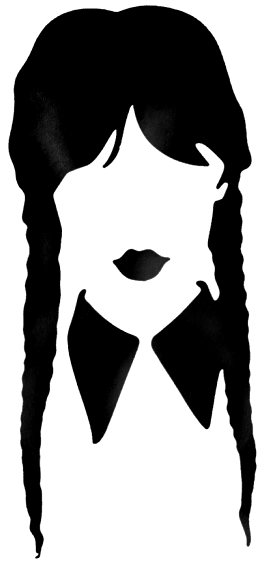
\includegraphics[height=1.35em]{figures/icons/mira-silhouette.png}}{}}}\enspace{\scshape\color{black}Scene}\enspace\textperiodcentered\enspace{\bfseries #1}\pdblockheadingend{\itshape #2}}%
    \end{tcolorbox}\par\addvspace{8pt plus 2pt}%
  }%
  \long\def\xrefbox#1{\par\pd@settle\addvspace{4pt}\noindent\pd@marginhead{See also}{\small #1}\par\addvspace{4pt}}%
  % A generic "Thesis" margin label does not identify which claim matters.
  % Keep the prose; use an authored keyidea head only when it adds meaning.
  \long\def\pdthesis#1{\par\pd@settle\addvspace{6pt plus 1pt}\noindent#1\par\addvspace{6pt plus 1pt}}%
  \long\def\pullquote#1{\pdthesis{#1}}%
}
\makeatother

% Shared visual language for the Book's figures -- version 2.
% Twin: book/figures/pd-figure-language.tex (byte-identical; edit both).
% The standard behind it, the migration from v1 and the QA loop live in
% skills/tikz-diagram-craft/ (SKILL.md, references/figure-standard.md).
%
% This file defines voices, hues, weights and marks -- not layouts.  Every
% figure still chooses a grammar from its reader question.
%
% ===========================================================================
% 1.  THE TYPE LADDER.  Three voices, one size, each tied to a role.
%       pd title   bold      panel titles, row and actor heads, column heads
%       pd label   upright   node text, state names, axis titles, tick words,
%                            relation words on an edge, badge numerals
%       pd note    italic    the one annotation a figure is allowed
%     `pd tag` is the label voice knocked out of the page, for a word that
%     must sit near a rule.  `pd kind` (small caps) is a one- or two-word kind
%     tag, never a title.  Every piece of figure text is mixed case; \texttt
%     only for identifiers that are literally code; math mode for symbols.
%
% 2.  THE COLOUR SYSTEM.  Hue is meaning, and the meanings cross chapters.
%     The figure's own subject is drawn in the CHAPTER hue (`pd focus ...`),
%     resolved from \pdcurrentchaptercolor, which the Book sets per chapter;
%     a fragment declares its standalone fallback with \pdfigurehue{...}.
%     Anything else the figure names takes its concept hue:
%       pd truth       pdcobalt   kernel, truth, the thing being specified
%       pd legible     pdteal     legibility, digest, inspection
%       pd ready       pdhealth   ready, coordinated, admitted, passing
%       pd protocol    pdindigo   protocol, federation, the wire
%       pd identity    pdviolet   identity, continuity, a card, an ID
%       pd reputation  pdrust     reputation, trust earned over time
%       pd value       pdgold     economy, value, settlement, payment
%       pd breach      pderror    breach, refusal, revocation, correction
%       pd warn        pdamber    warning; rules and stripes only, never text
%     Each concept X yields X, X rule, X arrow, X state, X fill, X datum and
%     X label.  Two to four hues a figure; colour is always doubled by shape,
%     dash, weight or a word (breach and warn are dashed as well as coloured).
%
% 3.  THE WEIGHT LADDER.  Exactly three weights, .5 / .9 / 1.6 pt
%     (1 : 1.8 : 3.2).  .5: hairline, guide, tick, artifact edge, fill edge,
%     mark outline, badge.  .9: rule, arrow, state edge, concept arrow.
%     1.6: spine, focus rule, focus and concept state edges, concept rule.
%     A reader sees which line is the subject.  Tips scale with the stroke.
%
% 4.  THE SURFACE LADDER.  pd state (page ground, ink edge) < pd artifact
%     (page ground, grey edge, subordinate) < pd focus state and the concept
%     states (24 % tint, edged in the same hue).  Text is always ink.  A
%     terminal state has a double boundary; an automaton's states are circles
%     (`pd automaton state/focus/terminal`); a ledger's pools are buckets
%     joined by pipes (`pd bucket`, `pd pipe`); a trust boundary is a dashed
%     rectangle (`pd trust boundary`).
%
% 5.  THE GROUND.  Body pages print on white, so every knockout and every
%     neutral surface is `pdpage` (white), never cream: a cream backing on a
%     white page reads as a sticker, which is what v1's figures were covered
%     in.  Neutral regions (Gantt bands, wells) are a warm grey tint.
%
% 6.  EDITIONS.  The Book sets \pdedition (maritime | swiss | technical) and
%     figures/pd-figure-language-<edition>.tex restyles the same names, so one
%     drawing renders in each edition's character.  A fragment that names a
%     raw colour (hhteal, pdcobalt!40, blue) bypasses this; name a role.
% ===========================================================================
% Libraries every v2 mark needs (diamonds, braces, markings), and
% pgfplots for computed plots. This file is \input in every preamble (the
% Book's and each standalone chapter's), so a plot works in all of them.
\usetikzlibrary{arrows.meta,matrix,patterns.meta,positioning,calc,fit,
  backgrounds,shapes.geometric,shapes.multipart,shapes.misc,decorations.pathreplacing,
  decorations.markings,quotes,intersections}
\RequirePackage{pgfplots}
\pgfplotsset{compat=1.18}
\usepgfplotslibrary{fillbetween,groupplots}

\colorlet{pdpage}{white}

% --- the chapter hue, resolved late --------------------------------------
% \pdfigurehue{pdindigo} on the line before a tikzpicture names the hue the
% figure is drawn in when it is compiled outside the Book (a standalone
% chapter, or the skill's renderer).  Inside the Book the preamble has already
% defined \pdcurrentchaptercolor and the chapter opener sets it, so there the
% opener wins and \providecommand does nothing.  Local to the figure's group.
\newcommand{\pdfigfraghue}{pdcobalt}
\newcommand{\pdfigurehue}[1]{%
  \renewcommand{\pdfigfraghue}{#1}%
  \providecommand{\pdcurrentchaptercolor}{#1}}
\newcommand{\pdsetfocushue}{%
  \ifdefined\pdcurrentchaptercolor
    \colorlet{pdfocus}{\pdcurrentchaptercolor}%
  \else
    \colorlet{pdfocus}{\pdfigfraghue}%
  \fi}
\colorlet{pdfocus}{pdcobalt}

% ===========================================================================
% THE TYPOGRAPHIC LAW
% ===========================================================================
% Companion to the line-weight law in figures/pd-palette.tex (1px texture,
% 1.5px linework, 2px enclosure). Same shape of rule: name the roles, fix the
% values, one place.
%
% ONE SIZE. Every named text role in a figure is \pdfiglabelsize
% (= \footnotesize). Roles separate by WEIGHT, SLOPE, FAMILY and INK -- never
% by size. A fragment never writes a size command of its own; if a distinction
% needs making, it takes the role that makes it.
%
% Where the size comes from. Measured, not chosen:
%   \tiny  \scriptsize  \footnotesize  \small  \normalsize
%   5.23    6.97          8.72           9.55    10.46  pt   Book (10.5pt
%                                                            Pagella, 4.5in
%                                                            column, 7x10in)
%   5.98    7.97          8.97           9.96    10.91  pt   standalone chapter
%                                                            (11pt Latin Modern)
% \scriptsize renders at 6.97pt in the Book -- under figcheck's 7pt T1 floor
% before a single width promotion, so it is illegal by measurement, not taste.
% \footnotesize holds 8.72pt and still clears the floor at the 0.85 \resizebox
% limit craft-rules sets (7.41pt). It is also what the corpus already voted
% for: 78 of the 91 local font= declarations this law replaces were already
% \footnotesize, \footnotesize\bfseries or \footnotesize\itshape.
%
% \pdfigbasesize (= \small) is the tikzpicture's ambient size only, so an
% unstyled node is never SMALLER than a styled one; every named role steps
% down exactly one notch from it and none steps down twice.
%
% ONE FACE, AND IT IS THE DOCUMENT'S. \pdfiglabelfamily is empty by default,
% which means figure type inherits whatever face the document is setting --
% Palatino in the Book, Computer Modern in a standalone chapter. Figures
% agreeing with EACH OTHER is not the goal; figures agreeing with the
% paragraph beside them is. A fragment therefore never names a family. Not
% \sffamily (which resolves to Latin Modern Sans against a Computer Modern
% page and reads as a foreign object on it), not \rmfamily, not
% \fontfamily{...}. P18 in tikz_precheck.py is an error for exactly that.
% An edition MAY substitute a face -- the Swiss and technical editions set
% \pdfiglabelfamily to \pdgrotesk, because grotesk display is their declared
% character -- and it does so in ONE command in ONE file, so the substitution
% is a decision on the record rather than an accident in a fragment. The
% only family a fragment may ask for is the identifier one, and it asks for
% it by role (pd mono label / \pdfiglabelmono), never by \ttfamily.
%
% What the roles are, and what each one is for:
%   pd panel title        bold        the name of a panel
%   pd row label          bold        an actor/row name east of its lane
%   pd reverse row label  bold, cream a row name sitting on a dark band
%   pd axis label         regular     an axis title or a tick numeral
%   pd direct label       regular     a value or name riding its own mark
%   pd reverse label      regular, cream  a direct label on a dark band
%   pd mono label         mono        an identifier, path, or literal
%   pd verdict            bold        a terminal outcome stamp (CLEAR, REJECT)
%   pd note               italic      one aside per figure
%   pd legend             regular     a pgfplots legend entry
%   pd state / terminal / actor / artifact / decision   node text
%   pd axis               the whole pgfplots typographic block, one key
%   \pdfigsub             a gloss line under a heading INSIDE a node
%   \pdfigmath            math carrying a sub/superscript, inside a label
%
% A fragment that needs a compound style of its own composes it from a role
% above (`gate/.style={pd decision,minimum width=2cm}`), or, where no role
% fits, from the \pdfiglabel* handles here. It never writes a raw size
% command: P16 in skills/harbor-chartwork/scripts/tikz_precheck.py is an
% error for exactly that, and P10/P11 have been errors for \tiny and
% \scriptsize since before this law.
%
% What does NOT transfer from the screen rules these roles otherwise follow.
% The dataviz method those rules come from assumes an interactive chart: a
% tooltip carries any value a label could not fit, a filter row rescopes the
% view, hover lifts the hovered mark. A printed page has none of that, and the
% absence is not a defect to design around. The INTENT of the tooltip rule --
% "every value is reachable without gating" -- does transfer, and on this page
% it is discharged somewhere else: the value is in the caption, in the margin
% apparatus, or in the chapter's own worked example. So a label that will not
% fit inside its mark moves outside the mark or is dropped to the caption; it
% is never shrunk to fit, because there is no size below \footnotesize to shrink
% to, and never clipped. Do not add a hover affordance, a legend toggle, or a
% filter to a figure in this book.
%
% IDENTIFIERS GET ONE SPELLING. A key, a cell id, a file name or any other
% literal a reader could type is set in `pd mono label` (or \pdfiglabelmono
% inside a compound style), spelled exactly as the code spells it: sk_A, not
% skA and not sk with a subscript A; card0, not card-nought and not a Unicode
% subscript zero. A figure that shows the same identifier two ways has told
% the reader they are two things. The subscripted form belongs to MATHEMATICS
% ($\kappa_7$, an index into a sequence) and the literal form to CODE -- one
% figure may use both, for different objects, but never both for the same
% one. (A precheck for two spellings of one identifier inside a fragment is
% being added on another branch; this is the convention it will enforce.)
%
% SHAPE IS A CHANNEL, AND IT HAS TO SURVIVE THE PRINT SIZE. pd datum, pd
% focus datum and pd caution datum carry three different forms, because the
% house palette is three low-chroma print inks and every distinction it makes
% has to be doubled by something that is not colour. That only counts if the
% form is still legible at 2.1-2.7 pt: an edition that flattens all three to
% one form has removed the second channel and left the figure separating its
% classes by hue alone, which fails in greyscale and for a colour-blind
% reader. Any edition override that restyles a datum must keep three
% distinguishable forms, and must be checked on a render at 1.0x, not
% reasoned about from the point sizes.
%
% One screen rule that does NOT bind here, and why. "Text never wears the data
% colour" exists because a light categorical hue is illegible as text on a
% light surface. The house figure hues are print inks, not screen hues --
% hhink #1B1712, hhteal #00564C, hhamber #6B4500 -- and all three clear text
% contrast on cream, so a label MAY wear its series' ink to bind itself to a
% curve, which is direct labelling and saves a legend. The rule that survives
% is the reason behind it: text wears one of those three inks at full
% strength, or hhink!80!hhgray for recessive furniture, and nothing else. A
% tint of an ink (text=hhgray, text=hhteal!60) is not a role; it is a fade.
% ===========================================================================

\providecommand{\pdfiglabelfamily}{}            % an edition may set \pdgrotesk
\providecommand{\pdfiglabelsize}{\footnotesize} % every named text role
\providecommand{\pdfigbasesize}{\small}         % the picture's ambient size
\providecommand{\pdfiglabel}{\pdfiglabelfamily\pdfiglabelsize}
\providecommand{\pdfiglabelbold}{\pdfiglabel\bfseries}
\providecommand{\pdfiglabelitalic}{\pdfiglabel\itshape}
\providecommand{\pdfiglabelmono}{\pdfiglabelsize\ttfamily}
% The one role that is not a node style, because it lives INSIDE a node's text:
% the second line under a heading that glosses it ("reviewer role / obligation +
% capability + authority"). Every fragment that needed it reached for \tiny or
% \scriptsize, which is how seven \tiny and twelve \scriptsize survived P10/P11
% as hard errors in the corpus. It steps down by SLOPE and WEIGHT, not size, so
% it stays legible and stays legal, and it touches neither family nor ink --
% which is what lets it sit on a reversed node without vanishing.
\providecommand{\pdfigsub}{\mdseries\itshape}
% The one place the law's own size is not the right size.
%
% Measured, both preambles, on a subscripted label inside `pd direct label`:
%
%              base glyph   subscript   subscript as % of base
%   chapter      8.97pt       5.98pt            66.7%
%   Book         8.72pt       6.36pt            72.9%
%   promoted    10.91/10.46   7.97/7.64
%
% An earlier version of this comment said those subscripts are "under figcheck's
% 7pt T1 floor". They are not, and the correction is worth more than the claim
% was. T1 has TWO bands: running text is held to 7.0pt, and a span of three
% glyphs or fewer -- a sub/superscript, a tick numeral -- is held to 5.9pt
% (T1_SHORT_SPAN_PT). That second band is not a loophole. A subscript is set at
% roughly 70% of its base by every typesetter that has ever existed; holding one
% to the running-text floor would mean either no subscripts in figures at all,
% or a figure whose base type is 10pt against 8.72pt body text.
%
% So \pdfigmath is NOT a T1 remedy, and using it as one is how a rule gets
% applied where it does not belong. It exists because 5.98pt clears the
% short-span band by 0.08pt, and 0.08pt is not a margin: a font substitution, an
% edition that nudges \pdfigbasesize, or a chapter that loads a different math
% font puts that subscript under the band with nobody having decided anything.
% Promotion puts it at 7.97/7.64pt -- over even the running-text floor -- while
% the base glyph stays close enough to its neighbours that the label still reads
% as one label.
%
% Use it ONLY for a math group that carries a sub- or superscript. Plain math
% takes the label's own size like any other text, and P22 in tikz_precheck.py is
% an error if it does not.
\providecommand{\pdfigmath}{\normalsize}

% ---------------------------------------------------------------------------
% THE GUIDE DASH, IN ABSOLUTE POINTS, IN ONE PLACE.
%
% `pd guide` used to read `line width=.45pt,densely dotted`. `densely dotted`
% expands to `dash pattern=on \pgflinewidth off 1pt`, and \pgflinewidth is read
% when the KEY is processed, not when the path is stroked. So the Swiss
% edition's `pd guide/.append style={draw=hhink!40,line width=.5pt}` widened the
% stroke and left the dash at the .45pt already baked into it. The canonical
% Book therefore shipped a 0.448pt dot on a 0.498pt stroke.
%
% MEASURED IN THE SHIPPED ARTIFACT, not in a probe: 50 guide strokes sampled
% pixel by pixel in the committed coordination-papers-mega-volume.pdf, at 150
% dpi / 1.0x.
%
%   on 0.448pt = 0.93 device px -- UNDER ONE PIXEL; off 0.996pt = 2.08 px
%   the dash DECLARES 69% of each line's length as gap
%   only 34% of each line's pixels actually reach paper
%   35.4% of three-period windows contain NO pixel that reaches paper at all
%
% That last number is the defect. The gap (2.08 px) is narrower than the
% antialias spread of a 0.93 px stroke, so as the pattern's phase drifts along a
% line the gaps fill in: over a third of every guide's length there is no gap
% left and it is a continuous grey stroke, while the rest of the same line still
% reads as dots. The ink arrives. The DOTTEDNESS does not. A reader sees one
% line that is dotted here and solid there, and no author chose that.
%
% Twenty-five of the corpus's thirty-six guide draws use dottedness to mean
% "this line is not a drawn edge", so twenty-five of them were making a
% distinction the page does not carry.
%
% After, same measurement, same probe geometry, Book preamble:
%   on 1.2pt = 2.50 px, off 2.0pt = 4.17 px, stroke .7pt = 1.45 px
%   0.0% of three-period windows are without paper -- every gap survives,
%     at every phase
%   50% of pixels reach paper against 62.5% declared, the shortfall now being
%     the stroke's antialias skirt rather than the whole signal
%
% ON THE INK, because the obvious reading of this change is wrong. The BASE pair
% was never the problem: hhgray!62 against the hairline's hhgray!78 is 0.411
% against 0.517 of nominal ink, well apart. The problem is that the Book renders
% the SWISS edition (\pdedition defaults to swiss; the committed Book PDF is
% full of hhink!40 guides), where the pair was hhink!40 against hhink!45 -- 4.6%
% of the grey scale. Deleting the Swiss override, which is the right fix for the
% geometry, makes the base ink govern the Book too -- and hhgray!62 is 0.411
% against the Book hairline's 0.410. The same grey, to a thousandth. So the base
% ink has to move, or the dash would go back to carrying the whole distinction
% by itself, which is how this started.
%
% hhink!70 measured against the hairline, mean ink on the page at 150 dpi:
%   chapter  guide 0.0502  hairline 0.0790   guide is 64% of the hairline
%   Book     guide 0.0545  hairline 0.0671   guide is 81% of the hairline
% Per DOT it is 0.638 against 0.410 -- unmistakably a different mark. In MEAN it
% is still lighter than the hairline -- so it still recedes. Two channels, both
% working, instead of one that does not.
%
% The replacement is stated absolutely and measures phase-STABLE: every dot
% renders at the same weight wherever it falls on the grid (peak column ink
% 0.808, invariant across twelve sub-pixel offsets). It is a macro rather than
% three numbers because an edition that restates one of them and not the others
% is how this defect happened. The geometry is a LEGIBILITY FLOOR, not an
% edition's character: an edition may move the guide's ink, and states the
% geometry through these two macros so it cannot half-restate it.
%
% Any dash in this corpus is stated in absolute points. The `dotted` family
% (`dotted`, `densely dotted`, `loosely dotted`) derives its on-length from the
% line width and is therefore banned -- P23 in tikz_precheck.py. `dashed` and
% its relatives are absolute (on 3pt off 3pt) and are fine.
\providecommand{\pdguidewidth}{.7pt}
% Three lengths, not one macro holding the whole key: pgfkeys splits a key list
% on `,` and `=` before expanding anything (so a macro carrying `dash
% pattern=...` is read as one key NAME), and TikZ's dash-pattern scanner reads
% the literal words `on`/`off` without expanding a macro that hides them. A
% dimension after each word does expand, which is the seam that works.
\providecommand{\pdguideon}{1.2pt}
\providecommand{\pdguideoff}{2.0pt}

\tikzset{
  % --- picture level: one size, one default tip, the chapter hue -----------
  % A figure label is a name, not prose: it never hyphenates.
  pd figure/.style={font=\pdfiglabelfamily\pdfigbasesize,text=pdink,line cap=round,line join=round,
    >={Stealth[length=2.6pt 3.2,width=2.0pt 2.4]},/utils/exec=\pdsetfocushue,
    every node/.append style={execute at begin node={%
      \hyphenpenalty=10000\exhyphenpenalty=10000\relax}}},
%
  % --- 1. the voices ---------------------------------------------------------
  pd title/.style={font=\pdfiglabelbold,text=pdink,align=center},
  pd label/.style={font=\pdfiglabel,text=pdink,align=center},
  pd note/.style={font=\pdfiglabelitalic,text=pdinkmuted,align=left},
  pd kind/.style={font=\pdfiglabel\scshape,text=pdinkmuted,align=center},
  pd tag/.style={pd label,fill=pdpage,inner sep=1.7pt},
%
  % --- 4. surfaces -----------------------------------------------------------
  pd state/.style={pd label,draw=pdink,line width=.9pt,fill=pdpage,
    rounded corners=1pt,inner xsep=6pt,inner ysep=4.5pt,minimum height=7.4mm},
  % a terminal state carries a double boundary, as every automaton text draws it
  pd terminal/.style={pd state,double=pdpage,double distance=1.1pt,line width=.5pt},
  pd artifact/.style={pd label,draw=pdinkmuted!60,line width=.5pt,fill=pdpage,
    rounded corners=1pt,inner xsep=5pt,inner ysep=3.5pt,minimum height=6.2mm},
  pd panel/.style={draw=pdinkmuted!55,line width=.5pt,
    dash pattern=on 2.4pt off 2pt,rounded corners=2.5pt,inner sep=7pt,align=center},
  pd hatch/.style={pattern={Lines[angle=45,distance=4pt,line width=.3pt]},
    pattern color=pdinkmuted!70},
  pd neutral fill/.style={fill=pdinkmuted!12,draw=pdinkmuted!55,line width=.5pt},
%
  % --- 3. strokes ------------------------------------------------------------
  pd hairline/.style={draw=pdinkmuted!45,line width=.5pt},
  % Absolute dash, from the typographic law's three macros above: a guide is a
  % definite dotted construction line, darker per dot than the hairline and
  % lighter in mean ink. A lattice is the quiet continuous grid a figure stands on.
  pd guide/.style={draw=pdink!70,line width=\pdguidewidth,dash pattern=on \pdguideon off \pdguideoff},
  pd lattice/.style={draw=pdinkmuted!40,line width=.4pt},
  pd tick/.style={draw=pdinkmuted!75,line width=.5pt},
  pd rule/.style={draw=pdink,line width=.9pt},
  pd spine/.style={draw=pdink,line width=1.6pt},
  pd thin arrow/.style={draw=pdinkmuted!75,line width=.5pt,->},
  pd arrow/.style={pd rule,->},
  pd spine arrow/.style={pd spine,->},
%
  % --- the chapter hue, as the figure's focus --------------------------------
  pd focus rule/.style={draw=pdfocus,line width=1.6pt},
  pd focus arrow/.style={pd focus rule,->},
  pd focus state/.style={pd state,draw=pdfocus,line width=1.6pt,fill=pdfocus!24},
  % The single solid chapter-colour surface in a figure: use only for the
  % culmination or object the reader should name after five seconds. Editions
  % may render ordinary focus with a pale field while keeping this one solid.
  pd climax state/.style={pd focus state},
  % a member of the subject's set when the set, not one node, is the subject:
  % edged in the chapter hue, never filled, so the one solid node stays unique
  pd focus outline/.style={pd state,draw=pdfocus,line width=1.2pt,fill=pdpage},
  pd focus fill/.style={fill=pdfocus!24,draw=pdfocus,line width=.5pt},
  pd focus datum/.style={circle,fill=pdfocus,draw=pdpage,line width=.5pt,inner sep=2.6pt},
  pd focus label/.style={pd label,text=pdfocus!85!pdink},
%
  % --- marks -----------------------------------------------------------------
  pd datum/.style={circle,fill=pdink,draw=pdpage,line width=.5pt,inner sep=2.3pt},
  pd badge/.style={pd label,circle,draw=pdink,line width=.5pt,fill=pdpage,
    inner sep=.5pt,minimum size=5.0mm},
  pd focus badge/.style={pd badge,draw=pdfocus,line width=.9pt,fill=pdfocus!24},
  % --- conventions shared by every chapter (Critical Analysis, 2026-09-08) ---
  % Automata: states are circles, terminal (accepting) states double circles;
  % edge words are short action names; guards go in an aligned legend table.
  pd automaton state/.style={pd label,circle,draw=pdink,line width=.9pt,fill=pdpage,
    minimum size=11mm,inner sep=1pt},
  pd automaton focus/.style={pd automaton state,draw=pdfocus,line width=1.6pt,fill=pdfocus!24},
  pd automaton terminal/.style={pd automaton state,double=pdpage,double distance=1.1pt,
    line width=.5pt},
  pd initial/.style={draw=pdink,line width=.9pt,->},
  % Ledgers: asset pools are rectangular buckets (open at the top) joined by
  % directed pipes; the conserved sum is set as an equation under the rails.
  pd bucket/.style={pd label,draw=none,minimum width=2.2cm,minimum height=1.3cm,
    append after command={\pgfextra{\draw[draw=pdink,line width=.9pt]
      (\tikzlastnode.north west) -- (\tikzlastnode.south west)
      -- (\tikzlastnode.south east) -- (\tikzlastnode.north east);}}},
  pd pipe/.style={draw=pdink,line width=.9pt,double=pdpage,double distance=2.2pt,
    -{Stealth[length=3.4pt 2,width=5.2pt]}},
  pd focus pipe/.style={pd pipe,draw=pdfocus},
  % Trust boundaries: a dashed rectangle is the Dolev-Yao interface; a vector
  % that escapes it is drawn in pd breach and named.
  pd trust boundary/.style={draw=pdink,line width=.9pt,dash pattern=on 4pt off 2.4pt,
    rounded corners=0pt,inner sep=8pt},
  % a stroke that ends at a badge is shortened, so no rule touches the numeral
  pd to badge/.style={shorten >=2pt},
  pd from badge/.style={shorten <=2pt},
}

% ===========================================================================
% 7.  PLOTS.  A plot is computed by a committed script, never sketched.  `pd
%     axis` is the one axis grammar: two spines (left, bottom), ticks out, no
%     box, no grid unless asked (`pd grid`), tick words in the label voice,
%     numbers with a thin-space thousands separator, room outside the plot for
%     direct labels (clip=false).  Series are named at their ends, not in a
%     legend: `pd series` (ink), `pd focus series` (chapter hue), and
%     `pd X series` for a concept; breach and warn series are dashed.  A
%     region between curves is `pd focus fill`/`X fill` with fillbetween.
%     Width: `width=` is the plot box (scale only axis); leave about 1.6 cm
%     of the 11.4 cm column for the y tick words and title.
% ===========================================================================
\pgfplotsset{
  pd axis/.style={
    scale only axis,width=8.8cm,height=4.6cm,
    axis lines*=left,axis line style={draw=pdink,line width=.5pt,-},
    tick align=outside,major tick length=3pt,minor tick length=0pt,
    tick style={draw=pdink,line width=.5pt},
    tick label style={pd label,text=pdinkmuted},
    label style={pd label},title style={pd title},
    every axis title/.append style={yshift=-2pt},
    enlargelimits=false,clip=false,
    grid=none,
    legend style={draw=none,fill=none,font=\pdfiglabel},
    /pgf/number format/1000 sep={\,},
    every axis plot/.append style={line width=.9pt,line join=round,mark size=1.7pt},
  },
  pd grid/.style={ymajorgrids,major grid style={draw=pdinkmuted!30,line width=.4pt}},
  pd series/.style={draw=pdink,mark=*,mark options={fill=pdink,draw=pdpage,line width=.5pt,solid}},
  pd focus series/.style={draw=pdfocus,line width=1.6pt,mark=*,
    mark options={fill=pdfocus,draw=pdpage,line width=.5pt,solid}},
  pd muted series/.style={draw=pdinkmuted!70,line width=.9pt,mark=none},
}
\newcommand{\pdplotconcept}[2]{%
  \pgfplotsset{#1 series/.style={draw=#2,mark=*,
    mark options={fill=#2,draw=pdpage,line width=.5pt,solid}}}}
\pdplotconcept{pd truth}{pdcobalt}
\pdplotconcept{pd legible}{pdteal}
\pdplotconcept{pd ready}{pdhealth}
\pdplotconcept{pd protocol}{pdindigo}
\pdplotconcept{pd identity}{pdviolet}
\pdplotconcept{pd reputation}{pdrust}
\pdplotconcept{pd value}{pdgold}
\pgfplotsset{
  pd breach series/.style={draw=pderror,dash pattern=on 3.2pt off 2.2pt,mark=diamond*,
    mark options={fill=pderror,draw=pdpage,line width=.5pt,solid}},
  pd warn series/.style={draw=pdamber,dash pattern=on 3.2pt off 2.2pt,mark=none},
}

% ===========================================================================
% Supplied visual-guide primitives: native Book type, deliberate strokes,
% readable Stealth heads, open markers, and a quiet quantitative grid.
% These are opt-in: old diagrams need spacing review before thicker arrows.
\tikzset{
  pd guide step/.style={pd artifact,draw=pdink,fill=pdpage,line width=1pt,
    align=center,minimum height=40pt,inner xsep=5pt,inner ysep=6pt},
  pd guide arrow/.style={draw=pdcobalt,line width=1.15pt,
    -{Stealth[length=7pt,width=4.4pt]},shorten <=2pt,shorten >=2pt},
}
\newcommand{\pdflowstep}[4]{%
  \node[pd guide step,text width=#4] (#1) at #2 {#3};}
\newcommand{\pdflowlink}[2]{%
  \draw[pd guide arrow] (#1.east)--(#2.west);}
\pgfplotsset{
  pd evidence axis/.style={pd axis,
    axis line style={draw=pdink,line width=1pt,-},
    tick style={draw=pdink,line width=.8pt},
    grid=major,major grid style={draw=pdinkmuted!20,line width=.35pt},
    axis background/.style={fill=pdpage}},
  pd evidence measured/.style={draw=pdcobalt,line width=1.35pt,mark=*,
    mark size=2.6pt,mark options={fill=pdpage,draw=pdcobalt,line width=1.1pt}},
  pd evidence comparison/.style={draw=pdink,line width=1.1pt,
    dash pattern=on 4pt off 2.5pt,mark=square*,mark size=2.2pt,
    mark options={fill=pdink,draw=pdink,solid}},
}
% Analytic curves, not sampled observations. Integer samples preserve the
% meaning of reviewer count; callers set axes and name their assumptions.
\newcommand{\pdindependentmisses}[2]{%
  \addplot[pd evidence measured,domain=1:#2,samples=#2] {100*(1-#1)^x};}
\newcommand{\pdreviewcost}[1]{%
  \addplot[pd evidence measured,domain=1:#1,samples=#1] {x};}
% 8.  UML.  The Book's engineering diagrams use UML 2.5 notation, so a reader
%     who knows UML reads them without a key.  Four kinds:
%     STATE MACHINE  `pd uml state` (rounded), `pd uml focus state`, a
%       composite drawn with `pd uml composite` around its substates plus a
%       compartment of internal transitions; `pd uml initial` (filled dot),
%       `pd uml final` (bullseye), `pd uml choice` (diamond); transitions are
%       `pd uml transition` (open arrowhead) labelled  event [guard] / effect.
%     SEQUENCE  `pd uml head` (lifeline head), `pd uml lifeline` (dashed),
%       `pd uml activation` (thin bar), messages `pd uml sync` (filled head),
%       `pd uml async` (open head), `pd uml reply` (dashed, open head),
%       `pd uml fragment` + `pd uml fragment tag` for alt / opt / loop.
%     COMPONENT  `pd uml component` with \pdumlicon{node} (the component
%       glyph) and a <<component>> keyword; `pd uml port`; provided interface
%       \pdumlprovided{from}{to}{name} (lollipop), required \pdumlrequired (socket).
%     ERD (crow's foot)  `pd er entity` (rectangle split: name, then rows;
%       mark keys PK / FK in the row text), relationship lines `pd er rel`
%       with tips `er one`, `er many`, `er zero or one`, `er one or many`,
%       `er zero or many` at either end.
% ===========================================================================
\pgfdeclarearrow{
  name = pd crow,
  parameters = {\the\pgfarrowlength,\the\pgfarrowwidth},
  setup code = {%
    \pgfarrowssettipend{0pt}%
    \pgfarrowssetlineend{0pt}%
    \pgfarrowssetbackend{-\pgfarrowlength}%
    \pgfarrowsupperhullpoint{0pt}{.5\pgfarrowwidth}%
    \pgfarrowsupperhullpoint{-\pgfarrowlength}{0pt}%
    \pgfarrowssavethe\pgfarrowlength
    \pgfarrowssavethe\pgfarrowwidth},
  drawing code = {%
    \pgfsetdash{}{0pt}%
    \pgfpathmoveto{\pgfqpoint{-\pgfarrowlength}{0pt}}%
    \pgfpathlineto{\pgfqpoint{0pt}{.5\pgfarrowwidth}}%
    \pgfpathmoveto{\pgfqpoint{-\pgfarrowlength}{0pt}}%
    \pgfpathlineto{\pgfqpoint{0pt}{-.5\pgfarrowwidth}}%
    \pgfusepathqstroke},
  defaults = {length=2.4mm, width=3.0mm}
}
\tikzset{
  % state machine
  pd uml state/.style={pd state,rounded corners=4.5pt},
  pd uml focus state/.style={pd focus state,rounded corners=4.5pt},
  pd uml terminal/.style={pd terminal,rounded corners=4.5pt},
  pd uml composite/.style={draw=pdink,line width=.9pt,rounded corners=7pt,fill=none,inner sep=0pt},
  pd uml initial/.style={circle,fill=pdink,draw=none,minimum size=2.4mm,inner sep=0pt},
  pd uml final/.style={circle,draw=pdink,line width=.9pt,fill=pdpage,minimum size=3.6mm,inner sep=0pt,
    path picture={\fill[pdink] (path picture bounding box.center) circle (1.1mm);}},
  pd uml choice/.style={diamond,draw=pdink,line width=.9pt,fill=pdpage,minimum size=4.2mm,inner sep=0pt},
  pd uml transition/.style={pd rule,-{Straight Barb[length=2.2pt 2.2,width=4.4pt 2.2]}},
  pd uml focus transition/.style={pd focus rule,-{Straight Barb[length=2.2pt 2.2,width=4.4pt 2.2]}},
  pd uml breach transition/.style={pd rule,draw=pderror,dash pattern=on 3.2pt off 2.2pt,
    -{Straight Barb[length=2.2pt 2.2,width=4.4pt 2.2]}},
  % sequence
  pd uml head/.style={pd state,rounded corners=0pt,minimum height=6.8mm},
  pd uml lifeline/.style={draw=pdinkmuted!75,line width=.5pt,dash pattern=on 3pt off 2pt},
  pd uml activation/.style={draw=pdink,line width=.5pt,fill=pdpage,minimum width=2.2mm,inner sep=0pt},
  pd uml sync/.style={pd rule,-{Triangle[length=3.2pt 1.6,width=3.2pt 1.6]}},
  pd uml async/.style={pd rule,-{Straight Barb[length=2.4pt 2,width=4.4pt 2]}},
  pd uml reply/.style={pd rule,dash pattern=on 3pt off 2pt,-{Straight Barb[length=2.4pt 2,width=4.4pt 2]}},
  pd uml fragment/.style={draw=pdink,line width=.5pt,fill=none,inner sep=6pt},
  pd uml fragment tag/.style={pd label,font=\footnotesize\bfseries,draw=pdink,line width=.5pt,fill=pdpage,
    inner xsep=3pt,inner ysep=2pt,chamfered rectangle,chamfered rectangle corners=south east,
    chamfered rectangle xsep=2pt},
  % component
  pd uml component/.style={pd state,rounded corners=0pt,align=center,inner xsep=8pt,inner ysep=6pt,minimum height=11mm},
  pd uml port/.style={rectangle,draw=pdink,line width=.5pt,fill=pdpage,minimum size=2mm,inner sep=0pt},
  % ERD
  pd er entity/.style={pd label,rectangle split,rectangle split parts=2,rectangle split part align={center,left},
    draw=pdink,line width=.9pt,fill=pdpage,inner xsep=5pt,inner ysep=3pt,align=left,
    rectangle split part fill={pdinkmuted!12,pdpage}},
  pd er rel/.style={pd rule},
  er one/.tip={Bar[width=3.0mm,sep=1.2pt]Bar[width=3.0mm]},
  er many/.tip={Bar[width=3.0mm,sep=1.4pt]pd crow},
  er zero or one/.tip={Circle[open,length=1.8mm,width=1.8mm,sep=1.2pt,fill=pdpage]Bar[width=3.0mm]},
  er one or many/.tip={Bar[width=3.0mm,sep=1.4pt]pd crow},
  er zero or many/.tip={Circle[open,length=1.8mm,width=1.8mm,sep=1.2pt,fill=pdpage]pd crow},
}
% the component glyph, drawn in the top-right corner of a component node
\newcommand{\pdumlicon}[1]{%
  \begin{scope}[shift={($(#1.north east)+(-4.2mm,-2.6mm)$)},x=1mm,y=1mm]
    \draw[pdink,line width=.5pt,fill=pdpage] (0,-1.1) rectangle (2.6,1.1);
    \draw[pdink,line width=.5pt,fill=pdpage] (-.6,.25) rectangle (.6,.65);
    \draw[pdink,line width=.5pt,fill=pdpage] (-.6,-.65) rectangle (.6,-.25);
  \end{scope}}
% a provided interface (lollipop) from a node side to a point, with its name
\newcommand{\pdumlprovided}[3]{%
  \draw[pd rule] (#1) -- (#2);
  \draw[pd rule,fill=pdpage] (#2) circle (1.3mm);
  \node[pd label,anchor=south] at ($(#2)+(0,1.6mm)$) {#3};}
% a required interface (socket): a half-circle open toward the provider
\newcommand{\pdumlrequired}[4]{% from, to, name, facing angle of the socket's opening
  \draw[pd rule] (#1) -- (#2);
  \draw[pd rule] ($(#2)+(#4+90:1.9mm)$) arc[start angle=#4+90,end angle=#4+270,radius=1.9mm];
  \node[pd label,anchor=north] at ($(#2)+(0,-2.4mm)$) {#3};}

% --- 2. the concept map, as styles, so a drawing never chooses a hue --------
% An edition file may \renewcommand\pdconcept before the map below expands.
\newcommand{\pdconcept}[2]{%
  \tikzset{%
    #1/.style={draw=#2,text=pdink},
    #1 rule/.style={draw=#2,line width=1.6pt},
    #1 arrow/.style={draw=#2,line width=.9pt,->},
    #1 state/.style={pd state,draw=#2,line width=1.6pt,fill=#2!24},
    #1 fill/.style={fill=#2!24,draw=#2,line width=.5pt},
    #1 datum/.style={circle,fill=#2,draw=pdpage,line width=.5pt,inner sep=2.6pt},
    #1 label/.style={pd label,text=#2!85!pdink},
  }}

% --- 6. the edition layer, loaded before the concept map expands ----------
\ifdefined\pdedition\IfFileExists{figures/pd-figure-language-\pdedition.tex}{\input{figures/pd-figure-language-\pdedition}}{}\fi

\pdconcept{pd truth}{pdcobalt}
\pdconcept{pd legible}{pdteal}
\pdconcept{pd ready}{pdhealth}
\pdconcept{pd protocol}{pdindigo}
\pdconcept{pd identity}{pdviolet}
\pdconcept{pd reputation}{pdrust}
\pdconcept{pd value}{pdgold}
\pdconcept{pd breach}{pderror}
\pdconcept{pd warn}{pdamber}
% Breach and warning read as refusals, so they are dashed as well as
% coloured, and a breach mark is a diamond where every other mark is a circle.
% Amber is never text (3.71:1 on white); a warn label is set in ink.
\tikzset{
  pd breach rule/.append style={dash pattern=on 3.2pt off 2.2pt},
  pd breach arrow/.append style={dash pattern=on 3.2pt off 2.2pt},
  pd warn rule/.append style={dash pattern=on 3.2pt off 2.2pt},
  pd warn arrow/.append style={dash pattern=on 3.2pt off 2.2pt},
  pd breach datum/.append style={diamond},
  pd warn label/.style={pd label},
}

% ===========================================================================
% v1 NAMES.  Kept so every existing fragment still compiles; they resolve to
% the v2 roles, so an untouched figure inherits the ladder.  New work uses the
% v2 names (skills/tikz-diagram-craft/references/migration-v1-to-v2.md).
% ===========================================================================
\tikzset{
  pd row label/.style={pd title,anchor=east},
  pd panel title/.style={pd title,align=left},
  pd axis label/.style={pd label},
  % Direct labels sit beside their mark; they do not erase a line or box
  % underneath themselves. A label that needs a paper knockout is misplaced
  % and must be moved, not given an invisible patch.
  pd direct label/.style={pd tag,fill=none,align=left},
  pd actor/.style={pd state},
  pd boundary/.style={pd panel},
  pd caution rule/.style={pd breach rule},
  pd caution arrow/.style={pd breach arrow},
  pd caution fill/.style={pd breach fill},
  pd caution datum/.style={pd breach datum},
}

% ===========================================================================
% Roles named on main by the typographic law (#10191), expressed on the v2
% roles so an edition's .append style on the parent reaches them. `pd danger`
% is main's name for what v2 calls `pd breach` (red, dashed, diamond marks);
% both names resolve to one family. Main's hairline-boxed fact badge is
% `pd fact badge`: v2's `pd badge` is the numbered guard/step marker.
% ===========================================================================
\tikzset{
  pd danger rule/.style={pd breach rule},
  pd danger arrow/.style={pd breach arrow},
  pd danger fill/.style={pd breach fill,text=pdink},
  pd danger datum/.style={pd breach datum},
  pd ink fill/.style={fill=pdink,draw=pdink,line width=.4pt,text=pdpage},
  pd decision/.style={pd state,diamond,aspect=1.55,font=\pdfiglabelbold,
    minimum height=0pt,inner xsep=3pt,inner ysep=3pt},
  pd mono label/.style={pd direct label,font=\pdfiglabelmono,inner xsep=2.5pt,inner ysep=2.5pt},
  pd verdict/.style={pd direct label,font=\pdfiglabelbold},
  pd reverse label/.style={pd direct label,text=pdpage,fill=none},
  pd reverse row label/.style={pd row label,text=pdpage},
  pd legend/.style={font=\pdfiglabel,text=pdink,draw=none,fill=none},
  pd kind tag/.style={pd kind,align=right},
  pd fact badge/.style={pd hairline,font=\pdfiglabel,text=pdink,align=center,
    inner sep=2.4pt,fill=none},
}

% Small reusable marks.  They deliberately avoid prose-bearing boxes.
\newcommand{\pdfigaxis}[4]{%
  \draw[pd rule,->] (#1,#2) -- (#3,#2);
  \node[pd label,anchor=west] at (#3,#2) {#4};
}
\newcommand{\pdfigvaxis}[4]{%
  \draw[pd rule,->] (#1,#2) -- (#1,#3);
  \node[pd label,anchor=south] at (#1,#3) {#4};
}

% Native-size, object-based evidence figures; shared by Book and chapters.
% Shared approved Swiss evidence drawing primitives. Keep both chapter roots identical.
\ifdefined\pdSwissEvidenceLoaded\else
\def\pdSwissEvidenceLoaded{1}
% Real ink-box gate; no declared coordinate envelope can substitute for this.
\newsavebox{\sgEvidenceBox}
\newcommand{\SGMeasuredFigure}[2]{%
  \sbox{\sgEvidenceBox}{#2}%
  \typeout{SG-GEOMETRY: #1,width=\the\wd\sgEvidenceBox,height=\the\dimexpr\ht\sgEvidenceBox+\dp\sgEvidenceBox\relax}%
  \ifdim\wd\sgEvidenceBox>325.215pt
    \PackageError{swiss-evidence}{Figure #1 exceeds the Book column}{Recompose at native text size; do not scale.}%
  \fi
  \usebox{\sgEvidenceBox}}
% Parent redraws after rejection of lab specimens 01,04,06.
% All coordinates are physical TeX points; no resizebox or transformed fonts.
\usetikzlibrary{arrows.meta,calc}
% Aliased onto the house palette (figures/pd-palette.tex), not \definecolor'd
% as independent HTML values: an edition that restyles pdcobalt/pdteal/...
% now restyles every SG figure with it. The six values were already
% bit-identical matches for pdcobalt/pdteal/pdviolet/pdamber/pderror/pdink;
% the alias turns that into a guarantee instead of a coincidence.
\colorlet{sgBlue}{pdcobalt}
\colorlet{sgTeal}{pdteal}
\colorlet{sgViolet}{pdviolet}
\colorlet{sgAmber}{pdamber}
\colorlet{sgRed}{pderror}
\colorlet{sgInk}{pdink}
\definecolor{sgGrid}{HTML}{D8C7A6}
% The one house size, inheriting the document's own face (the typographic
% law in pd-figure-language.tex): no \sffamily leak, no local \fontsize.
\newcommand{\SGType}{\pdfiglabel}
\tikzset{sg/base/.style={x=1pt,y=1pt,line cap=butt,line join=miter,
  every node/.style={font=\SGType,inner sep=0pt,text=sgInk}},
  sg/arrow/.style={-{Stealth[length=4.5pt,width=3.6pt]},draw=sgInk,line width=.85pt},
  sg/grid/.style={draw=sgGrid,line width=.3pt},
  sg/hash/.style={draw=sgBlue,fill=sgBlue!7,line width=1pt,minimum width=53pt,
    minimum height=27pt,inner sep=4pt,align=center},
  sg/sibling/.style={draw=sgAmber,fill=sgAmber!10,line width=1pt,minimum width=51pt,
    minimum height=27pt,inner sep=4pt,align=center},
  sg/check/.style={draw=sgInk,fill=white,line width=1pt,minimum width=92pt,
    minimum height=30pt,inner sep=5pt,align=center}}

% A folded record, not an undifferentiated rounded node. Width/height are pt.
\newcommand{\SGDocument}[6]{%
  \begin{scope}[shift={#2}]
    \path[draw=sgInk,fill=#5,line width=.85pt]
      (0,0)--({#3-7},0)--(#3,7)--(#3,#4)--(0,#4)--cycle;
    \draw[sgInk,line width=.65pt] ({#3-7},0)--({#3-7},7)--(#3,7);
    \node[minimum width=#3pt,minimum height=#4pt,text width=\dimexpr#3pt-12pt\relax,
      align=center] (#1) at ({#3/2},{#4/2}) {#6};
  \end{scope}}

\newcommand{\SGSurvival}{%
\begin{tikzpicture}[sg/base]
  % Three complete probability decades, percentages rather than tiny exponents.
  \foreach \x in {0,1,...,6}{\draw[sg/grid] ({35+30*\x},20)--({35+30*\x},140);}
  \foreach \y/\lab in {20/{0.1\%},60/{1\%},100/{10\%},140/{100\%}}{%
    \draw[sg/grid] (35,\y)--(215,\y);
    \draw[sgInk,line width=.65pt] (32,\y)--(35,\y);
    \node[anchor=east] at (28,\y) {\lab};}
  \draw[sgInk,line width=.85pt] (35,140)--(35,20)--(215,20);
  \foreach \x in {0,2,4,6}{%
    \draw[sgInk,line width=.65pt] ({35+30*\x},20)--({35+30*\x},17);
    \node[anchor=north] at ({35+30*\x},12) {$\x$};}
  \node[rotate=90] at (-9,80) {jobs still running (log scale)};
  \node[anchor=north] at (125,-5) {duration / mean duration};
  \draw[sgBlue,line width=1.5pt,domain=0:6,samples=100]
    plot ({35+30*\x},{140-120*ln(1+\x/2)/ln(10)});
  \draw[sgViolet,line width=1.2pt,dash pattern=on 4pt off 2.5pt,domain=0:6,samples=100]
    plot ({35+30*\x},{140-40*\x/ln(10)});
  % Endpoint leaders have allocated space; text does not lie on a curve.
  \draw[sgBlue,line width=.8pt] (215,67.75)--(224,67.75);
  \node[anchor=west,text=sgBlue,font=\SGType\bfseries] at (230,73) {Lomax};
  \node[anchor=west,text=sgBlue] at (230,60) {1.56\%};
  \draw[sgViolet,line width=.8pt,dashed] (215,35.77)--(224,35.77);
  \node[anchor=west,text=sgViolet,font=\SGType\bfseries] at (230,40) {exponential};
  \node[anchor=west,text=sgViolet] at (230,27) {0.248\%};
\end{tikzpicture}}

\newcommand{\SGTiming}{%
\begin{tikzpicture}[sg/base,y=-1pt]
  % This bracket spans COMMIT TO SYNC. It is not a range of hypothetical syncs.
  \path[draw=sgAmber!35,fill=sgAmber!9,line width=.5pt] (39,19) rectangle (253,49);
  \draw[sgAmber,line width=1pt] (39,18)--(39,9)--(253,9)--(253,18);
  \node[anchor=south,text=sgAmber,font=\SGType\bfseries] at (146,5) {?};
  \draw[sgInk,line width=.9pt] (39,27)--(39,45) (253,27)--(253,45);
  \draw[{Stealth[length=4.5pt,width=3.6pt]}-{Stealth[length=4.5pt,width=3.6pt]},
    sgAmber,line width=1.3pt] (40,36)--(252,36);
  \node[anchor=north,font=\SGType\bfseries] at (39,52) {commit};
  \node[anchor=north,font=\SGType\bfseries] at (253,52) {WAL sync};
  \node[anchor=west] at (0,86) {heartbeats received};
  \foreach \x/\label in {57/{s_1},117/{s_2},194/{s_3},278/{s_4}}{%
    \draw[sgViolet!70,dashed,line width=.55pt] (\x,104)--(\x,145);
    \node[anchor=south,text=sgViolet] at (\x,101) {$\label$};}
  \path[draw=sgAmber!35,fill=sgAmber!9,line width=.5pt] (158,108) rectangle (243,142);
  \draw[sg/grid] (0,139)--(306,139);
  \draw[sgTeal,line width=1.4pt]
    (0,132)--(25,132)--(25,116)--(33,116)--(33,132)
    --(85,132)--(85,116)--(93,116)--(93,132)
    --(145,132)--(145,116)--(153,116)--(153,132)--(306,132);
  \draw[sgRed,line width=1pt] (243,106)--(243,145);
  \node[anchor=north,text=sgRed] at (243,149) {deadline};
  \draw[sg/arrow] (0,174)--(306,174);
  \node[anchor=north east] at (306,179) {time};
\end{tikzpicture}}

\newcommand{\SGInclusion}{%
\begin{tikzpicture}[sg/base,y=-1pt]
  % Two independent inputs: a supplied proof and an issuer-authenticated root.
  \node[anchor=north west,font=\SGType\bfseries,text width=158pt,align=left] at (0,0)
    {Recompute from the receipt};
  \node[anchor=north west,font=\SGType\bfseries,text width=118pt,align=left] at (193,0)
    {Authenticate\\the checkpoint};
  \draw[sg/grid,step=15pt] (0,29) grid (175,194);
  \SGDocument{receipt}{(4,35)}{49}{34}{sgViolet!9}{receipt $P$}
  \node[sg/hash] (leaf) at (29,103) {$a=H_L(P)$};
  \node[sg/sibling] (sibone) at (108,103) {sibling $b$};
  \node[sg/hash] (inner) at (68,146) {$u=H_N(a,b)$};
  \node[sg/sibling] (sibtwo) at (146,146) {subtree $c$};
  \node[sg/hash,fill=sgBlue,text=white,minimum width=100pt] (computed) at (107,190)
    {$R'=H_N(u,c)$};
  \draw[sg/arrow,draw=sgViolet] (receipt.south)--(leaf.north);
  \draw[sg/arrow,draw=sgBlue] (leaf.south)--(inner.north west);
  \draw[sg/arrow,draw=sgAmber] (sibone.south)--(inner.north east);
  \draw[sg/arrow,draw=sgBlue] (inner.south)--(computed.north west);
  \draw[sg/arrow,draw=sgAmber] (sibtwo.south)--(computed.north east);
  \SGDocument{checkpoint}{(211,37)}{85}{48}{sgTeal!8}{signed root $R^*$\\size $n=4$\\signature $\sigma$}
  % The trusted key is an external input, not something the prover supplies.
  \draw[sgInk,line width=1pt] (218,113) circle (3.5pt);
  \draw[sgInk,line width=1pt] (221.5,113)--(233,113) (230,113)--(230,117) (233,113)--(233,117);
  \node[anchor=west] at (239,113) {trusted $pk_I$};
  \node[sg/check,minimum width=84pt] (verify) at (260,158) {verify $\sigma$\\result $A$};
  \draw[sg/arrow,draw=sgTeal] (checkpoint.east)--(311,61)--(311,158)--(verify.east);
  \draw[sg/arrow] (247,123)--(247,138)--(verify.north);
  \node[sg/check,minimum width=112pt,minimum height=34pt] (compare) at (164,245)
    {$A\ \land\ (R'=R^*)$};
  \draw[sg/arrow,draw=sgBlue] (computed.south)--(107,220)--(compare.north west);
  \draw[sg/arrow,draw=sgTeal] (verify.south)--(260,214)--(compare.north east);
  \node[anchor=east,text=sgTeal] at (250,204) {$R^*,A$};
  \node[draw=sgTeal,fill=sgTeal,text=white,minimum width=90pt,
    minimum height=27pt,font=\SGType\bfseries] (accept) at (76,299) {accept inclusion};
  \node[draw=sgRed,fill=white,text=sgRed,line width=1.2pt,minimum width=90pt,
    minimum height=27pt,font=\SGType\bfseries] (reject) at (256,299) {reject proof};
  \draw[sg/arrow,draw=sgTeal] (compare.south west)--(108,279)--(76,279)--(accept.north);
  \draw[sg/arrow,draw=sgRed] (compare.south east)--(220,279)--(256,279)--(reject.north);
  \node[anchor=south,text=sgTeal] at (82,275) {true};
  \node[anchor=south,text=sgRed] at (248,275) {false};
\end{tikzpicture}}

% Reusable geometry; load after swiss-redraws.tex. Real points, no scaling.
\newcommand{\SGDatabase}[4]{%
  \begin{scope}[shift={#2}]
    \path[draw=#3,fill=#3!7,line width=.9pt]
      (0,4)--(0,32) arc[start angle=180,end angle=360,x radius=24pt,y radius=5pt]
      --(48,4) arc[start angle=0,end angle=-180,x radius=24pt,y radius=5pt];
    \draw[draw=#3,fill=#3!7,line width=.9pt] (24,4) ellipse[x radius=24pt,y radius=5pt];
    \node[minimum width=48pt,minimum height=37pt,align=center] (#1) at (24,18) {#4};
  \end{scope}}

% Reader question: How do overlapping requests become ordered records?
% Evidence: schematic two-client history, not a runtime observation.
% Each request precedes commit 1; each reply follows its own committed record.
\newcommand{\SGWriterSequence}{%
\begin{tikzpicture}[sg/base,y=-1pt]
  % Recomposed at native size: a 22-character mono request label no longer
  % fits a 118pt lane gap at \pdfiglabelmono, so the HTTP verb is shortened
  % to the identifier it names and the resource it names ("auth.ts") moves
  % to the lane header, where it reads once instead of twice.
  \foreach \x/\lanelabel in {35/{{\pdfigmath$\alpha_{\text{auth}}$} (claude)},153/{Kernel (single writer)},275/{{\pdfigmath$\alpha_{\text{bill}}$} (codex)}}{
    \node[anchor=south,font=\pdfiglabelbold,align=center] at (\x,0) {\lanelabel};
    \draw[sg/grid] (\x,9)--(\x,237);}
  % Both invocations precede the first commit: overlapping client requests.
  \draw[sg/arrow,draw=sgViolet] (35,29)--(153,29);
  \node[anchor=south,text=sgViolet,font=\pdfiglabelmono] at (94,24) {POST /claims};
  \draw[sg/arrow,draw=sgAmber] (275,57)--(153,57);
  \node[anchor=south,text=sgAmber,font=\pdfiglabelmono] at (214,52) {POST /claims};
  % commit 1 succeeds: drawn in the kernel's own hue. commit 2 is the
  % kernel's WAL record of a REFUSAL, not a second grant -- it is drawn in
  % the breach hue so the outcome is doubled by colour, not stated in prose
  % alone (the typographic law's "colour is always doubled" rule). The
  % "lock held" highlight band is gone: at native size it ran directly
  % behind this text, which figcheck reads as a drawn line through the
  % words, and the sequencing arrows already carry the serialization claim.
  \SGDocument{commitA}{(93,71)}{120}{46}{sgBlue!8}{{\pdfiglabelbold commit 1 \textperiodcentered{} WAL 4102}\\[2pt]{\pdfigsub {\pdfigmath$\alpha_{\text{auth}}$} \textperiodcentered{} epoch 104}}
  \draw[sg/arrow,draw=sgViolet,dash pattern=on 3pt off 2pt] (153,130)--(35,130);
  \node[anchor=south,text=sgViolet,font=\pdfiglabel] at (94,128) {201 Created};
  \SGDocument{commitB}{(93,152)}{120}{46}{sgRed!8}{{\pdfiglabelbold commit 2 \textperiodcentered{} WAL 4103}\\[2pt]{\pdfigsub {\pdfigmath$\alpha_{\text{bill}}$} refused}}
  \draw[sg/arrow,draw=sgAmber,dash pattern=on 3pt off 2pt] (153,213)--(275,213);
  \node[anchor=south,text=sgAmber,font=\pdfiglabel] at (214,211) {409 Conflict};
  \draw[sg/arrow] (3,20)--(3,232);
  \node[anchor=west,font=\pdfiglabel] at (9,236) {time};
\end{tikzpicture}}

% Reader question: What is checked before the service admits requests?
% Source: SQLite WAL documentation, sections 2--2.2, cited in the chapter.
% Checkpointing copies committed pages; it does not apply uncommitted work.
% The dashed group denotes separate mechanisms, not a proved composition.
\newcommand{\SGRecoveryAdmission}{%
\begin{tikzpicture}[sg/base,y=-1pt]
  % Recomposed at native size: a 25-character mono command (sqlite3_wal_
  % checkpoint_v2) no longer fits a 103pt-wide column once the label grows
  % from 5.0pt to \pdfiglabelmono, so the three mechanisms read top to
  % bottom, full measure, instead of left to right in three narrow lanes.
  \draw[sgInk!55,dash pattern=on 3pt off 2pt,line width=.7pt]
    (0,0) rectangle (300,318);

  % 1. Checkpoint WAL
  \node[anchor=north west,align=left,text width=228pt] at (10,8)
    {{\pdfiglabelbold 1. Checkpoint WAL}\\[2pt]
     {\pdfiglabelmono\color{sgBlue} sqlite3\_wal\_checkpoint\_v2}\\[2pt]
     {\pdfigsub Copies committed WAL pages into the main database; uncommitted frames are not applied.}};
  \SGDocument{walback}{(247,4)}{34}{26}{sgViolet!7}{}
  \SGDocument{walfront}{(253,9)}{34}{26}{sgViolet!7}{WAL}
  \draw[sg/arrow] (18,101)--(18,118);

  % 2. Check Pages
  \node[anchor=north west,align=left,text width=228pt] at (10,122)
    {{\pdfiglabelbold 2. Check Pages}\\[2pt]
     {\pdfiglabelmono\color{sgTeal} PRAGMA integrity\_check}\\[2pt]
     {\pdfigsub Verifies B-tree pointers and freelist allocation across every page.}};
  \SGDatabase{db}{(251,118)}{sgBlue}{SQLite}
  \draw[sg/arrow] (18,215)--(18,232);

  % 3. Verify Links
  \node[anchor=north west,align=left,text width=228pt] at (10,236)
    {{\pdfiglabelbold 3. Verify Links}\\[2pt]
     {\pdfiglabelmono\color{sgAmber} Merkle chain verify}\\[2pt]
     {\pdfigsub Validates cryptographic audit-log continuity link by link.}};
  \foreach \x in {249,267,285}{
    \draw[sgAmber,line width=1pt,rounded corners=2pt] (\x,240) rectangle ({\x+14},256);}
  \draw[sgAmber,line width=1pt] (259,248)--(267,248) (281,248)--(289,248);

  % Decision Gate
  \node[sg/check,minimum width=165pt,minimum height=28pt,font=\pdfiglabelbold] (admit) at (150,350)
    {all critical checks pass?};
  \draw[sg/arrow] (150,318)--(admit.north);

  \node[draw=sgTeal,fill=sgTeal,text=white,minimum width=125pt,minimum height=32pt,
    align=center] (serve) at (65,420) {{\pdfiglabelbold admit requests}\\[1.5pt]{\pdfigsub HTTP 200 Ready (:9876)}};
  \node[draw=sgRed,fill=white,text=sgRed,line width=1pt,minimum width=125pt,
    minimum height=32pt,align=center] (refuse) at (235,420) {{\pdfiglabelbold refuse service}\\[1.5pt]{\pdfigsub HTTP 503 Unavailable}};

  \draw[sg/arrow,draw=sgTeal] (admit.south west)--(90,384)--(65,384)--(serve.north);
  \draw[sg/arrow,draw=sgRed] (admit.south east)--(210,384)--(235,384)--(refuse.north);
  % Each tag sits clear of its own diagonal leg, on the side the diagonal
  % does NOT occupy -- PASS left of its bend, FAIL right of its bend --
  % rather than centred on the bend where the stroke crosses the glyphs.
  \node[anchor=south east,text=sgTeal,font=\pdfiglabelbold] at (63,382) {PASS};
  \node[anchor=south west,text=sgRed,font=\pdfiglabelbold] at (237,382) {FAIL (HALT)};
\end{tikzpicture}}

% Named bands and their audiences; the dashed floor is NOT a fifth layer.
\newcommand{\SGStackLayers}{%
\begin{tikzpicture}[sg/base,y=-1pt]
  \foreach \y/\level/\name/\audience/\evidence/\hue in {
    0/3/Economy/{Between operators}/{settlement and reputation}/sgAmber,
    51/2/Legibility/{For the operator}/{summaries linked to evidence}/sgTeal,
    102/1/Coordination/{Between agents}/{permissions and commitments}/sgViolet,
    153/0/Substrate/{On one machine}/{ordered writes and records}/sgBlue}{
    \path[draw=\hue,fill=\hue!8,line width=1pt] (17,\y) rectangle (142,{\y+38});
    \node[anchor=west,font=\SGType\bfseries,text=\hue] at (26,{\y+13}) {L\level};
    \node[anchor=west,font=\SGType\bfseries] at (26,{\y+27}) {\name};
    \node[anchor=north west,font=\SGType\bfseries] at (158,{\y+2}) {\audience};
    \node[anchor=north west,text width=149pt,align=left] at (158,{\y+17}) {\evidence};}
  \foreach \y in {153,102,51}{\draw[sg/arrow] (79,\y)--(79,{\y-13});}
  \draw[sgBlue,line width=2.4pt] (7,154)--(7,190);
  \draw[sgInk!60,dashed,line width=.7pt] (17,204) rectangle (307,243);
  \node[anchor=west,font=\SGType\bfseries] at (26,216) {Machine floor};
  \node[anchor=west] at (26,231) {file lock, clock, socket, supervisor};
  \draw[sg/arrow] (79,204)--(79,192);
\end{tikzpicture}}

% Compact counterpart for future chapter-by-chapter marginal navigation.
% A named current-layer argument changes emphasis, never the layer order.
\newcommand{\SGMarginLadder}[1]{%
\begin{tikzpicture}[sg/base,y=-1pt]
  \foreach \y/\n/\name/\hue in {0/3/Economy/sgAmber,37/2/Legibility/sgTeal,74/1/Coordination/sgViolet,111/0/Substrate/sgBlue}{
    \draw[\hue,line width=.7pt] (0,\y)--(91,\y);
    \node[anchor=north west,text=\hue,font=\SGType\bfseries] at (4,{\y+3}) {L\n};
    \node[anchor=north west] at (4,{\y+16}) {\name};
    \ifnum\n=#1\relax\draw[\hue,line width=2pt] (0,{\y+3})--(0,{\y+29});\fi}
\end{tikzpicture}}

\fi



% Research-maturity scale: a neutral four-point grade for how far each claim sits
% from a verified, running artifact. Used inline in prose and tables.
%   implemented : exists, exercised, true under the production runtime
%   partial     : exists but holds under a narrower condition than the prose invites,
%                 or detects rather than prevents
%   specified   : a concrete design exists, but no running artifact realizes it
%   proposed    : named as a direction, with no design yet
% \Built, \BuiltWeak, \Designed, \Vision and \NotGuar -- and the
% \Closed/\Partial/\Open proof-obligation markers this chapter's status tables
% use -- are defined once, for this paper and for the Book, in
% figures/pd-pedagogy.tex (\input above). They used to be redefined here; a
% chapter preamble is discarded when the Book is assembled, so a local
% definition silently applied to the standalone paper only.

% (The legacy \pullquote, \keyidea and \pitfall tinted-box definitions used to
% sit here. They were dead code: figures/pd-pedagogy.tex re-\RenewDocumentCommand's
% \keyidea and \pitfall and re-\long\def's \pullquote from its own
% \AtBeginDocument block, so these preamble definitions never ran at render
% time. Removed rather than left as a cosmetic leftover.)


% ─── Listings Setup ──────────────────────────────────────────────────────────
\lstdefinestyle{proverif}{
  language=C,
  backgroundcolor=\color{codebg},
  frame=single,
  rulecolor=\color{codeframe},
  basicstyle=\ttfamily\small,
  keywordstyle=\color{hhink}\fontseries{b}\selectfont,
  commentstyle=\color{hhgray}\itshape,
  stringstyle=\color{hhgray},
  numbers=left,
  numberstyle=\tiny\color{gray},
  numbersep=8pt,
  breaklines=true,
  showstringspaces=false,
  tabsize=2,
  xleftmargin=15pt,
  xrightmargin=5pt,
  framexleftmargin=15pt,
  captionpos=b
}

\lstdefinestyle{pseudocode}{
  language=C,
  backgroundcolor=\color{codebg},
  frame=single,
  rulecolor=\color{codeframe},
  basicstyle=\ttfamily\small,
  keywordstyle=\color{hhink}\fontseries{b}\selectfont,
  commentstyle=\color{hhgray}\itshape,
  stringstyle=\color{hhgray},
  numbers=left,
  numberstyle=\tiny\color{gray},
  numbersep=8pt,
  breaklines=true,
  showstringspaces=false,
  tabsize=2,
  xleftmargin=15pt,
  xrightmargin=5pt,
  framexleftmargin=15pt,
  captionpos=b,
  morekeywords={function,return,if,then,else,for,while,do,begin,end,atomic,transaction,reject,commit,assert,raise}
}

\lstset{style=proverif}

% ─── Theorem Environments ────────────────────────────────────────────────────
\theoremstyle{definition}
\newtheorem{definition}{Definition}[section]
\newtheorem{theorem}{Theorem}[section]
\newtheorem{lemma}{Lemma}[section]
\newtheorem{property}{Property}[section]
\theoremstyle{remark}
\newtheorem*{remark}{Remark}

% ─── Header/Footer ───────────────────────────────────────────────────────────
\pagestyle{fancy}
\fancyhf{}
\fancyhead[L]{\small\itshape\color{hhgray} The Single-Writer Kernel}
\fancyhead[R]{\small\color{hhgray}\thepage}
\fancyfoot[C]{\footnotesize\color{hhgray} Port Daddy Coordination Papers \textperiodcentered\ Chapter~\pdchapternumber\ of \pdchaptercount}
\renewcommand{\headrulewidth}{0.4pt}
\renewcommand{\footrulewidth}{0pt}

% ─── Title ───────────────────────────────────────────────────────────────────
\title{
  \vspace{-1cm}
  {\Large\textsc{Port Daddy Coordination Papers --- Chapter~\pdchapternumber\ of \pdchaptercount}}\\[
0.5cm]
  \rule{\textwidth}{0.5pt}\\[0.3cm]
  {\LARGE\textbf{The Single-Writer Kernel:}}\\[0.2cm]
  {\Large A Local Transactional Reference Monitor\\for Agent Swarms}\\[0.3cm]
  \rule{\textwidth}{0.5pt}
}
\author{
  \textbf{Erich Owens}\\[0.2cm]
  Curiositech LLC\\[0.2cm]
  \texttt{engineering@portdaddy.dev}
}
\date{\pdeditiondate\\Version 1.2 (textbook edition)}
% ─── Document ────────────────────────────────────────────────────────────────
% Hyperlink and cross-reference discipline (must stay last in the preamble).
% Shared hyperlink and cross-reference discipline for the Book and its chapters.
% Load this LAST in every preamble: cleveref must follow hyperref and amsthm.
% hyperref itself is loaded earlier with [backref=page] (a load-time option).
% Twin copy under book/figures/ (byte-identical; checked by
% scripts/generate-mega-whitepaper.test.mjs).
%
% What a reader gets: live links on chapter titles, section numbers, theorems,
% figures, tables, equations, page numbers, and citations; PDF bookmarks three
% levels deep; and, at the end of every bibliography entry, the pages that cite it.
% Links are quiet: a warm dark ink one step lighter than body text, so the
% four part hues keep their meaning and an inline chapter title never competes
% with the part it sits in. Chrome pages (the front-matter map, part openers)
% recolor their own links locally.
\hypersetup{
  colorlinks=true,
  linkcolor=pdinkmuted,
  citecolor=pdinkmuted,
  urlcolor=pdinkmuted,
  filecolor=pdinkmuted,
  anchorcolor=pdink,
  bookmarksnumbered=true,
  bookmarksdepth=3,
  bookmarksopen=true,
  bookmarksopenlevel=1,
  breaklinks=true,
  linktoc=all,
  pdfauthor={Erich Owens},
  pdftitle={\pdchaptertitle},
  pdfsubject={\pdeditiontitle: \pdeditionsubtitle},
}

% Title-based chapter references. \pdchaplink{prefix}{text} is a live link to
% the chapter inside the Book (the Book's preamble defines it before loading this
% file); in a standalone chapter it is plain text. Prose uses \pdchapref, which
% sets the title in italics; the locator map uses \pdchaplink directly.
\providecommand{\pdchaplink}[2]{#2}
\DeclareRobustCommand{\pdchapref}[2]{\pdchaplink{#1}{\emph{#2}}}

% \ifpdbook -- true in the assembled Book, false otherwise.
%
% WHY THIS EXISTED. A drawing that two chapters both \input prints twice in the
% Book, under two figure numbers. The fix is for the chapter that develops the
% idea to keep the figure and the other to point at it -- but the standalone
% edition of a chapter had nowhere to point, and rewriting the prose outright
% removed five figures from harbor-economy-whitepaper.pdf and left it telling a
% conference reader that a ceremony is "drawn in The Federated Harbor", a
% document that reader did not have.
%
% WHERE IT STANDS NOW. The per-chapter PDFs are retired: the Book is the one
% document, so \ifpdbook is true in every build that renders, and the \else
% branches are source with no output. They are still here, and still read by
% check_duplicate_figures.py (which must not count an \else \input as a Book
% input) -- but nothing prints them, and nothing new should be put in one.
% Whether to delete them is an open question; see the retirement PR.
%
% The divergence was per-build. A CONDITIONAL and not a two-argument macro:
% the generator inlines each \input, so a figure branch is a whole table or
% tikzpicture, and as a macro argument that is scanned as one token list --
% which is how \pdinbook produced "runaway argument" on the first attempt.
% \ifpdbook skips the untaken branch at the TeX level instead.
%
% Declared unconditionally and defaulting FALSE, which is the standalone
% answer. The Book's preamble sets \pdbooktrue immediately after loading
% this file. A guard here would have to mention \ifpdbook or \newif inside a
% branch TeX may skip, and a conditional token in skipped text is counted as
% a nested \if -- which is how two attempts at a guard both produced
% "Incomplete \ifdefined". Ordering is cheaper than cleverness.
\newif\ifpdbook

% cleveref: "Theorem 3.1", "Figure 2.4", "Section 1.3", capitalised, never
% abbreviated, with the whole phrase clickable. Names are declared explicitly
% because the theorem environments are created before this file is loaded.
\usepackage[nameinlink,capitalise,noabbrev]{cleveref}
\crefname{pdchapter}{Chapter}{Chapters}
\crefname{part}{Part}{Parts}
\crefname{appendix}{Appendix}{Appendices}
\crefname{definition}{Definition}{Definitions}
\crefname{theorem}{Theorem}{Theorems}
\crefname{lemma}{Lemma}{Lemmas}
\crefname{proposition}{Proposition}{Propositions}
\crefname{corollary}{Corollary}{Corollaries}
\crefname{conjecture}{Conjecture}{Conjectures}
\crefname{property}{Property}{Properties}
\crefname{protocol}{Protocol}{Protocols}
\crefname{lsprotocol}{Protocol}{Protocols}
\crefname{stpprotocol}{Protocol}{Protocols}
\crefname{heprotocol}{Protocol}{Protocols}
\crefname{remark}{Remark}{Remarks}
\crefname{lstlisting}{Listing}{Listings}
\crefname{exercise}{Exercise}{Exercises}
\crefname{solution}{Solution}{Solutions}
\Crefname{pdchapter}{Chapter}{Chapters}
\Crefname{lstlisting}{Listing}{Listings}
\Crefname{exercise}{Exercise}{Exercises}
\Crefname{solution}{Solution}{Solutions}

% Back-references: "^ Cited on pages 12, 40, and 87." after every bibliography
% entry, each page number a live link back to the page that cited the work.
% Distinct pages only (#3/#4).
%
% The page numbers used to be wrapped in \color{hhgray} along with the words,
% which painted over the link colour hyperref had just given them: the links
% were there -- 29 annotations on a typical bibliography page -- and looked
% exactly like the grey prose around them, so nobody knew they could click.
% Restoring the quiet link colour would not have fixed it either; pdinkmuted
% against hhgray is 1.53:1, which is no signal at footnote size.
%
% So the numbers take pdcobalt (7.55:1 on the cream, and a hue a reader cannot
% mistake for grey), and the line opens with the return arrow this book already
% uses to send a solution back to its exercise. This is a deliberate exception
% to the quiet-link discipline above, and the reason is that back-matter
% navigation is the one place where the link IS the content: in prose the
% surrounding sentence tells you a phrase is a destination, and in a
% bibliography nothing does.
\renewcommand*{\backref}[1]{}
\renewcommand*{\backrefalt}[4]{%
  \ifcase #3\relax
  \or {\footnotesize{\color{hhgray}$\uparrow$~Cited on page}~{\hypersetup{linkcolor=pdcobalt}#4}{\color{hhgray}.}}%
  \else {\footnotesize{\color{hhgray}$\uparrow$~Cited on pages}~{\hypersetup{linkcolor=pdcobalt}#4}{\color{hhgray}.}}%
  \fi}
\renewcommand*{\backrefsep}{, }
\renewcommand*{\backreftwosep}{ and }
\renewcommand*{\backreflastsep}{, and }

\begin{document}
\pdopensolutions
\setlength{\emergencystretch}{2em}
\maketitle
\thispagestyle{empty}
\vspace{0.6cm}
\vspace{0.4cm}
\noindent\textbf{Keywords:} complete mediation, single-writer transactions, SQLite
write-ahead logging, durability by fault class, linearizability, deontic logic,
commitments, stigmergy, local-first coordination, multi-agent systems
\vspace{0.4cm}
\noindent\textit{Reading time: approximately 45 minutes end-to-end. This is Chapter~\pdchapternumber{} of \pdbooktitle{}, a
\pdchaptercountword-chapter textbook, and the chapter every later one rests on.
\pdchapref{ls}{The Legible Swarm} is the operator-facing entry point and a natural
place to start; \pdchapref{stp}{From Spawn to Person} builds an
identity-and-reputation bridge on top of this kernel; \pdchapref{he}{The Harbor
Economy} carries the cross-machine market, including
cross-machine capability transfer, which belongs to the cross-machine layer and
lives there, not here. Any chapter can be read first, but every later layer rests on
this one.}
\tableofcontents
\newpage
% ═════════════════════════════════════════════════════════════════════════════
\section{Where this chapter sits, and what it promises}
% ═════════════════════════════════════════════════════════════════════════════
Alice's two agents both want port 7421 for a development server. They need
one answer about who may use it, and they need that answer to survive an agent
exiting. Start with the record they can agree to consult.

\begin{pdexample}{Two requests, one recorded holder}
The claims table starts empty. Agent A requests port 7421 for 60 seconds;
the writer records A and confirms success. Agent B then requests the same
port before the lease expires. The writer reads the existing row and returns
``held by A,'' leaving one row, not two. If A repeats its request after a
lost reply, the same holder is returned; a retry does not create a second
ownership record. These are three requests and one holder [internal,
hand trace]. The record still cannot stop B from binding the port through an
unmediated operating-system call. It settles a question inside the service;
confinement is a further requirement.
\end{pdexample}

The \emph{daemon} is the background process answering these requests. A
\emph{transaction} groups database changes into an all-or-nothing step;
\emph{commit} is the point at which that step becomes part of the database's
accepted history. SQLite's \emph{write-ahead log} (WAL) records the changes
before they are copied into the main database file. A \emph{lease} is a
reservation with an expiry time. We return to these requests when we
consider ordering, crash recovery, and stale holders: each adds a condition
the simple trace has deliberately left open.

% Swiss object-based redraw; geometry lives in shared reusable functions.
% Evidence: corresponding single-writer-kernel.tex section; schematic, not a runtime trace.
\begin{figure}[H]
\centering
\SGMeasuredFigure{fig-swk-stack-map}{\SGStackLayers}
\caption{Read upward from L0. Higher layers depend on the records beneath them, but introduce their own assumptions. The blue tick identifies this chapter. The dashed box beneath L0, the machine, is a dependency, not a fifth layer.}
\label{fig:swk-stack-map}
\end{figure}

We model an agent-coordination system as a four-layer stack
(Figure~\ref{fig:swk-stack-map}), each layer serving a different \emph{whom}.
\begin{description}[leftmargin=2.2em,style=nextline]
\item[L0, storage (the machine).] A single always-on daemon over one local
database: it stores records durably and applies changes one at a time.
\emph{This chapter's core.}
\item[Coordination (the agents).] The protocol agents speak through the storage
layer: ownership claims, a message bus, shared signals that fade over time,
obligations, and policy enforcement. This chapter specifies the implemented
half of it.
\item[Legibility (the operator).] The human-facing view that renders the swarm
intelligible. Treated in an accompanying chapter (\emph{The Legible Swarm}).
\item[Economy (the market between operators).] The cross-machine market in which
operators trade work and reputation. Treated in an accompanying chapter (\emph{The
Harbor Economy}).
\end{description}
\noindent Later chapters depend on this kernel in different ways.
The operator's view reads its claims, its message bus, and its
\pdterm{policy monitor}, the component that checks recorded operations against
the rules.
Durable agent identity requires its continuity records. The settlement ledger
adds tables under the same writer, while cross-machine transfer uses its signed
record of who granted which permission to whom. A fault in these records can
therefore affect supervision, attribution, or settlement; each guarantee below
states the conditions it needs.
\subsection{The one-sentence thesis}
\pdthesis{The kernel is a single-writer transactional \pdterm{reference monitor},
a component that checks every change to protected state, over a local SQLite/WAL
database. One process accepts every change to coordination
state and records the order of those changes. Its ledger is authoritative for
those changes and for nothing else about the world outside it.}
The two guarantees require different qualifications:
\begin{enumerate}[leftmargin=1.4em]
  \item \textbf{Durability, with two exceptions:} a write that returned success
  survives the death of any agent and the death of the \emph{daemon process}.
  It may \emph{not} survive an operating-system crash or a power loss before the
  next checkpoint; \S\ref{sec:durability} states which failures it survives.
  \item \textbf{Mediation:} a guard that runs before a change takes effect can
  refuse a forbidden change. A monitor that runs afterwards can only report the
  change or respond to it. Refusing a forbidden change before it takes effect
  is called \pdterm{regimentation}. How fast a later monitor detects or repairs
  a violation depends on separate assumptions about timing and availability.
\end{enumerate}

\ifdefined\pdswisslandmarkplate
\begin{figure}[p]
  \centering
  \pdswisslandmarkplate{05}{\linewidth}
\end{figure}
\pdmarginpagebreak
\fi

\subsection{Why ``reference monitor,'' and why \emph{not} \mbox{consensus}}
The right mental model is the reference monitor of Anderson and
Lampson~\pdcite{anderson1972,lampson1974}: a component that checks every access
to protected state (\emph{always invoked}, or complete mediation), that other
programs cannot alter (\emph{tamper-resistant}), and that is \emph{small enough
to verify}. Here the reference monitor is a concrete local daemon over one
SQLite file. Over the kernel's own state, every change is checked \emph{by
construction}. Every change to \emph{coordination state} goes through one
writer, so the daemon puts the changes in one order and is the one place the
checks run; SQLite's file lock is a backstop. This is Saltzer and Schroeder's
``economy of mechanism''~\pdcite{saltzer1975protection}: one mechanism, with one
moving part, in place of $N$ hand-written critical sections. The checking is complete only over
writes that \emph{enter} the daemon. It does not cover what an agent running as
the same user can do \emph{beside} the daemon. A classical reference monitor is
always invoked because the hardware or operating system forces every access
through it. This kernel has no such boundary, so a process running as the same
user can change shared state the daemon never sees: it can edit a file under an
advisory claim, run \texttt{git} directly, or write the SQLite file itself.
Checking is therefore complete over the daemon's \emph{programming interface}
and advisory everywhere else. Making it complete over everything an agent can
do on the host needs enforcement outside the daemon. The threat model
(\S\ref{sec:threatmodel}) states that problem, and a kernel boundary under a
separate user, which does not yet exist (\S\ref{sec:enforcement-gap}), would
close it.
\pdmarginfigure{lampson}{Butler Lampson's access matrix: permissions connect subjects to objects.}%
\keyidea[One writer needs no consensus]{Many agents contending for shared
state, with failover, look like a distributed-systems problem, and the usual
reflex is Raft, Paxos or CRDTs. The kernel avoids that problem. With one writer
on one machine using one file, there is nothing for several processes to
\emph{agree} on, so the consensus impossibility result of Fischer, Lynch, and
Paterson~\pdcite{flp1985} does not apply. The design sidesteps the result without
solving it. Distribution across machines belongs to the economy layer; a
consensus protocol inside the local storage layer would be in the wrong layer.}
A local writer avoids the agreement protocol required by a replicated
system~\pdcite{kleppmann2017}. The conditional theorem in
\S\ref{sec:invariants} states the resulting guarantee: when every read and write goes
through the sole daemon connection one request at a time and responses follow commit,
transactions are \emph{serializable} and claim/lock operations are \emph{linearizable}
against a stated specification of leases that expire. Linearizability is what lets the
coordination layer treat ``who holds this'' as one authoritative record. Serializable
means the result matches some sequential transaction order. Linearizable adds
real-time order: a claim completed before another request began must appear
first. Overlapping requests may be ordered either way if their results fit
that order; the three-request port example will return in the claim-history
exercise.
\paragraph{Reading a mechanism's status.}
A theorem states its assumptions; an implementation grade says whether the
reference artifact realizes them. \Built{} means shipped and exercised by tests in the reference
implementation, \BuiltWeak{} means shipped but materially weaker than its name
suggests, \Designed{} means specified with a proof or a written protocol but
not yet shipped, and \Vision{} means a stated direction whose critical part
has no specification yet.
Appendix~\ref{app:status} gives the full key and artifact map. In the body,
keep two questions separate: which failures a record survives, and which
transitions a gate can prevent. The next sections work through both.

% ═════════════════════════════════════════════════════════════════════════════
\section{The kernel as seven subsystems}
\label{sec:organs}
% ═════════════════════════════════════════════════════════════════════════════
The kernel's seven \emph{subsystems} share one database but have distinct
contracts (Table~\ref{tab:swk-seven-organs}). Separating them makes it possible
to trace which guarantees depend on claims, sessions, messages, or policy
checks, and which failures cross subsystem boundaries.
\begin{table}[H]
\centering
\caption{The seven subsystems, each the contract the daemon holds for the layer above it,
with the table that is its home where the chapter names one and its maturity grade.
All seven are disciplines over one SQLite/WAL file: one commit history, not seven
stores. The grades come from the chapter's own status table (\S\ref{app:status}).}
\label{tab:swk-seven-organs}
\small
\renewcommand{\arraystretch}{1.15}
\begin{tabularx}{\textwidth}{@{}>{\raggedright\arraybackslash}p{0.22\textwidth} >{\raggedright\arraybackslash}X >{\raggedright\arraybackslash}p{0.21\textwidth}@{}}
\toprule
\textbf{Subsystem} & \textbf{Contract held for the layer above} & \textbf{Maturity} \\
\midrule
transactional store & one writer, one durable file; every other subsystem is a set of tables written through the same commit history & \Built \\
resource / exclusion & at most one compatible holder per conflict domain; leases expire and are swept lazily (home: \texttt{claims}) & \Built{} (exact keys); \BuiltWeak{} (file regions) \\
actor continuity & a stable actor identity across sessions, mechanically present but asserted by the actor, not proven & \BuiltWeak\ self-asserted \\
message carriage & an ordered, cursor-addressable, durable envelope delivered at least once (home: \texttt{messages}) & \Built \\
obligation \& enforcement & no \emph{done} without a receipt the daemon can re-check; the policy monitor detects and cannot always prevent (home: \texttt{commitments}) & \BuiltWeak \\
session memory & notes and events survive process death; execution state does not & \Built\ (memory) \\
self-attestation & the daemon reports its own coverage as enforced, degraded or stubbed, never silently & \Built \\
\bottomrule
\end{tabularx}
\end{table}
The \textbf{storage subsystem} lies under the other six; mechanically, they are
tables updated through the same SQLite connection. For example, accepting
A's claim changes the \texttt{claims} table, while recording A's promised
release changes \texttt{commitments}. They share a transaction mechanism
without making ownership and obligation the same fact. We examine storage,
resource exclusion, and commitment checking in detail, then use them to
explain communication and recovery.
\pdexercisepointer{\ref{ex:swk-organs-inmemory}}{\ref{ex:swk-organs-cut}}{\pageref{ex:swk-organs-inmemory}}
% ═════════════════════════════════════════════════════════════════════════════
\section{The storage subsystem: one writer, one file}
\label{sec:substrate}
% ═════════════════════════════════════════════════════════════════════════════
The storage subsystem makes two promises: a write that returned success is
durable, and changes are applied one at a time. This section covers the second
promise, the single-writer discipline. \S\ref{sec:durability} covers
durability, where the chapter makes its largest correction.
\subsection{The single-writer discipline}
% Swiss object-based redraw; geometry lives in shared reusable functions.
% Evidence: corresponding single-writer-kernel.tex section; schematic, not a runtime trace.
\begin{figure}[H]
\centering
\SGMeasuredFigure{fig-swk-single-writer}{\SGWriterSequence}
\caption{Both requests arrive before the first commit. The writer orders their records and replies after each commit. This sequence assumes one writer; it does not establish power-loss durability.}
\label{fig:swk-single-writer}
\end{figure}

\pdmarginanalogy{swk-one-printing-press}{}{one-printing-press}{Like our single-writer daemon, the platen handles jobs one after another.}
In the kernel (Figure~\ref{fig:swk-single-writer}), dozens of command-line
invocations and agent connections funnel their writes through one writer. That writer
is the daemon, the only process holding a read--write connection to the
database file. SQLite's operating-system file lock and a bounded busy-wait then
put all changes in order. Two mechanisms can do that ordering, and the
definition below says \emph{which} one the design relies on.
\begin{definition}[Single-writer discipline]\label{def:single-writer}
\setlength{\parskip}{4pt plus 1pt}
All state-mutating operations route through a single daemon process holding one
SQLite write connection.
Concurrency among the many clients (command-line
invocations, agents over the message transports, background workers) is resolved
by the daemon's request queue; the SQLite file lock is the \emph{backstop} that
preserves correctness if the discipline is ever violated by a second writer (for
example a stray direct write), not the primary serialization mechanism.
\end{definition}
\keyidea[Routing makes the writer unique]{``Single-writer'' is a rule about
routing: every write goes through the daemon. SQLite's file lock still orders
writes if that rule is broken. SQLite accepts several writer connections and
puts them in order instead of refusing them, so the property holds because of
where writes are routed; the database itself does not forbid a second writer.
The standing risk is a second \emph{copy} of the daemon opening the same file,
which is why the kernel also runs self-checks that detect a divergent or stale
second instance (\S\ref{sec:attest}).}
\subsection{The configuration \emph{is} the durability claim}
\ifpdmargincolumn\pdcheckpointwindow\fi
The storage configuration is short, and it decides the durability claim. In WAL mode with
the \emph{normal} synchronization level (the WAL is fsync'd at checkpoints rather
than on every commit), a bounded auto-checkpoint interval, a bounded busy-wait,
foreign-key enforcement on, and a clean-shutdown checkpoint-and-truncate, the
kernel inherits exactly the crash semantics that configuration defines. The claim
``a write that returned success survives a crash'' reduces \emph{entirely} to what
WAL with normal synchronization guarantees. \S\ref{sec:durability} shows that
this is less than a casual reading assumes.
\subsection{Schema evolution: an ordered boot ledger, not yet a sequencer (OP-7)}
\pdstatus{\BuiltWeak}{OP-7, the seventh of the chapter's numbered open problems (Table~\ref{tab:op-status}); the ordered boot ledger ships; the sequencer is specified}
The initial schema-by-union approach (\texttt{CREATE TABLE IF NOT EXISTS}) created
vulnerabilities around unsequenced renames and multi-column backfills. The kernel's
answer so far is partial, and it trades one property for another.
What ships is a \textbf{boot-time migration ledger}: the daemon applies
a numbered, totally ordered set of migrations before it serves any request, and then
\emph{verifies the schema it is about to serve from}: it probes the actual tables
and column sentinels instead of trusting that the statements ran without error,
and refuses to serve on a mismatch. That is a real fail-safe default: a
half-applied migration cannot quietly become part of the coordination record.
What does \emph{not} yet ship is the sequencer that would make that order
authoritative. Subsystem modules still self-initialize their own tables over the shared
database handle (Appendix~\ref{app:status}), so the schema is still, in part, a
union. A strict linear ledger managed exclusively by the daemon via SQLite's
\texttt{pragma user\_version}, in which modules \emph{declare} migrations rather
than applying them, is specified but not built. The schema-ordering question is
therefore answered in part: modules must follow an explicit dependency order,
giving up the ``any module, any order'' flexibility of schema-by-union, and the
daemon does not yet enforce that order everywhere.
Table~\ref{tab:swk-schema-evolution} states the trade in two rows.
\begin{table}[H]
\centering
\caption{Schema evolution (OP-7): what ships today against the sequencer the
design would still need. [internal]}
\label{tab:swk-schema-evolution}
\small
\renewcommand{\arraystretch}{1.2}
\begin{tabularx}{\textwidth}{@{}>{\raggedright\arraybackslash}p{0.22\textwidth} X@{}}
\toprule
\textbf{State} & \textbf{What governs migration order} \\
\midrule
ships (\BuiltWeak) & a numbered, totally ordered boot-time migration ledger, applied before any request is served, with post-apply verification against the actual tables; subsystem modules still self-initialize their own tables, so the schema is still, in part, a union \\
designed (\Designed) & a strict linear ledger managed exclusively by the daemon via \texttt{pragma user\_version}, in which modules \emph{declare} migrations rather than applying them themselves \\
\bottomrule
\end{tabularx}
\end{table}
\subsection{Path and ownership invariants}
The database resolves to a single canonical path with owner-only file permissions.
Signing-key isolation remains partial: operating-system keychain storage is an
unfinished requirement, and a same-user attacker remains outside the guarantee
(\S\ref{sec:threatmodel}). A fail-closed guard refuses to open the live registry
from a test, much as a web framework refuses to run its tests against the
production environment. This is Saltzer and Schroeder's \emph{fail-safe
defaults}~\pdcite{saltzer1975protection} applied at the one place a test could
corrupt the live record.
\subsection{The second writer: one record across several machines}
\label{sec:second-writer}
\pdstatus{\Designed}{writer transfer between harbors; the local single writer is built}
A team may run several machines, each with its own kernel governing its own
agents (each such governed environment is a \emph{harbor}), and want one shared
plan across them: which objectives are authorized, who owns what, which
changes were accepted. A shared service could either display copies of each
machine's record or become the one place where that record is written; it must
not do both. A copy of this kind, a \pdterm{projection}, can be searched and
displayed anywhere, but writing to it changes nothing. Exactly one process at a
time is the writer whose accepted changes define the record. Handing the writer
role to another process is recorded by raising an authority number, the
\emph{epoch}, and any write stamped with an older epoch is refused. This
handover is designed but not yet implemented.
Under the proposed signing policy, the harbor signs work intents with its own
key; a relay verifies and applies them but cannot author them. A snapshot feed
that replaces a remote mirror while leaving the local daemon authoritative is
still only a projection, and replicating that feed does not transfer writing
authority. The single-writer implementation supports this rule for one harbor;
no code yet exercises it across harbors.
The proposed writer transfer is a procedure of six steps, in this order. (1) Freeze: the local harbor stops accepting writes and records the
freeze as its last transition. (2) Export: the ledger and its root hash leave
the harbor as one artifact. (3) Verified import: the receiving authority
imports the artifact and proves, against the root, that what it holds is what
left. (4) Check: projections and permissions are re-derived on the new side
and compared with the old. (5) Epoch: the new writer's epoch is signed and
published, and every client refuses a write under any older epoch from that
moment. (6) Rollback only by another epoch: there is no return to the old
writer except by running the same procedure in reverse, so the record never
has two writers, even for the duration of a mistake. A flag would not do, for
the same reason revocation needs an epoch in \pdchapref{anchor}{The Anchor
Protocol}. The model-checked attack there restores a backup taken before a
revocation and so resurrects a dead credential, bringing a revoked one back
into use; it fails only
when stored state carries the epoch under which it was valid. A restored
harbor database that predates the handover is the same attack against the
writer role, and the same defence stops it. The argument is a
\emph{model-checked property} for credentials and a \emph{design invariant}
for writers; nothing in the repository yet checks the writer case.
\begin{pdboundary}
\setlength{\parskip}{4pt plus 1pt}
The alternative the procedure exists to forbid is dual writing with
reconciliation: both authorities accept writes for a while and \mbox{receipts}
reconcile them afterwards. That gives two records that can disagree, which
every result in this chapter assumes cannot happen. No receipt repairs it
afterwards, because the receipt itself would need a writer.
A transfer implementation must demonstrate
that an interrupted cutover or restored backup cannot reactivate a stale writer,
and that the new epoch was authorized by the existing root of authority.
The local ledger does not provide those checks. Until the transfer is
implemented and checked, a remote copy remains a projection of the local
records.
\end{pdboundary}
\pdexercisepointer{\ref{ex:swk-schema-rename}}{\ref{ex:swk-op7-sequencer}}{\pageref{ex:swk-schema-rename}}
% ═════════════════════════════════════════════════════════════════════════════
\section{Durability, split by fault class}
\label{sec:durability}
% ═════════════════════════════════════════════════════════════════════════════
\paragraph{One acknowledged write, two failures.}
Heron records a claim on port~7421 for the checkout test server and a note
naming the revision under repair. Both writes return success. Now fork the
same history at a moment before the next synchronization to stable storage.
If only the daemon process dies, the operating system's page cache survives;
SQLite can recover the committed claim and note when the daemon restarts.
If the host loses power, that cache may disappear too: the database can remain
consistent while those recent acknowledged writes are lost.

Figure~\ref{fig:swk-durability-dramatization} asks what survives each fork.
Heron received an acknowledgement in both cases. What differs is which
component still held the acknowledged bytes. Neither case recovers an edit or
thought Heron never recorded.

% II/fig:swk-durability-dramatization -- parent recomposition.
% Question: what changes when the same acknowledged commit meets two faults?
% Claim: losing only the process preserves the OS/WAL state; losing volatile
% state can lose a recent unsynchronized commit. Five milliseconds is illustrative.
% Grammar: one common storage state, then two aligned fault/outcome rows.
% Required: acknowledgment, WAL/NORMAL, cache versus stable storage, same fault
% instant, conditional survival, I1a Built / I1b NotGuar, no post-power-loss sync.
% Reject: elapsed time as proof of missing sync; a checkpoint invocation as a
% durability certificate; two already-durable outcomes; cache and disk conflation.
\begin{figure}[H]
\centering
\SGMeasuredFigure{swk-durability-dramatization}{%
\begin{tikzpicture}[pd figure,x=1pt,y=1pt,
  dur label/.style={pd label,align=center,inner sep=0pt},
  dur head/.style={dur label,font=\pdfiglabelbold},
  dur flow/.style={-{Stealth[length=4pt,width=3pt]},draw=pdink,line width=.7pt}]
  \node[dur head,anchor=west] at (0,95) {$t_0$: commit acknowledged};
  % The folded record names the chapter's concrete objects, not a new schema.
  \path[draw=pdink,line width=.7pt,fill=pdviolet!5]
    (0,26) -- (0,75) -- (63,75) -- (75,63) -- (75,26) -- cycle;
  \draw[draw=pdink,line width=.7pt] (63,75) -- (63,63) -- (75,63);
  \node[dur label,text width=58pt] at (35,49) {claim\\+ note};
  \draw[dur flow] (79,49) -- (105,49);
  \path[draw=pdink!60,fill=pdcreamraised,line width=.6pt] (120,31) rectangle (193,71);
  \path[draw=pdink!60,fill=pdpage,line width=.6pt] (113,26) rectangle (186,66);
  \node[dur label,text width=62pt] at (149.5,47) {WAL in\\OS cache};
  \draw[dur flow,dashed,draw=pdgold] (199,49) -- (251,49);
  % Stable storage is a distinct destination, not another cache sheet.
  \path[draw=pdink,fill=pdcreamraised,line width=.7pt]
    (260,60) -- (260,34) arc[start angle=180,end angle=360,x radius=28,y radius=7]
    -- (316,60);
  \draw[draw=pdink,fill=pdcreamraised,line width=.7pt] (288,60) ellipse[x radius=28,y radius=7];
  \node[dur label,text width=62pt] at (287,14) {stable storage};
  \node[dur label,text width=111pt,text=pdgold,anchor=south] at (251,79)
    {sync not established};
  \node[dur label,anchor=west,text=pdinkmuted] at (0,5) {WAL / NORMAL};
  \draw[draw=pdink!25,line width=.4pt] (0,-13) -- (321,-13);

  % Same fault instant for both alternatives. The row positions are not time.
  \node[dur head,text width=90pt] at (43,-32) {Fault at $t_0+5\,\mathrm{ms}$};
  \node[dur head,text width=90pt] at (151,-32) {Volatile state};
  \node[dur head,text width=106pt] at (268,-32) {On restart};
  \path[fill=pdteal!5] (0,-95) rectangle (321,-47);
  \path[fill=pdteal] (0,-95) rectangle (2,-47);
  \node[dur label,text width=78pt] at (43,-71) {daemon\\killed};
  \draw[dur flow,draw=pdteal] (88,-71) -- (104,-71);
  \node[dur label,text width=82pt] at (151,-71) {OS/cache\\intact};
  \draw[dur flow,draw=pdteal] (197,-71) -- (213,-71);
  \node[dur head,text width=98pt,text=pdteal] at (268,-64) {record survives};
  \node[dur label,text width=98pt] at (268,-82) {I1a: implemented};

  \path[fill=pdrust!5] (0,-156) rectangle (321,-108);
  \path[fill=pdrust] (0,-156) rectangle (2,-108);
  \node[dur label,text width=78pt] at (43,-132) {power\\lost};
  \draw[dur flow,draw=pdrust] (88,-132) -- (104,-132);
  \node[dur label,text width=82pt] at (151,-132) {cache\\erased};
  \draw[dur flow,dashed,draw=pdrust] (197,-132) -- (213,-132);
  \node[dur head,text width=98pt,text=pdrust] at (268,-125) {record may be lost};
  \node[dur label,text width=98pt] at (268,-143) {I1b: not guaranteed};
\end{tikzpicture}%
}
\caption{With OS and database/WAL state intact, restart recovers a process-crash commit; power loss can erase an unsynchronized commit. The five-millisecond interval is illustrative.}
\label{fig:swk-durability-dramatization}
\end{figure}

Durability is a claim about a named failure class. Table~\ref{tab:swk-durability-faultclass} summarizes the two forks and the stronger synchronization policy.
\begin{table}[H]
\centering
\caption{WAL: \texttt{NORMAL} survives process crashes. \texttt{FULL} adds
per-commit synchronization against OS crashes and power loss. [internal]}
\label{tab:swk-durability-faultclass}
\small
\renewcommand{\arraystretch}{1.2}
\begin{tabularx}{\textwidth}{@{}>{\raggedright\arraybackslash}p{0.24\textwidth} *{3}{>{\centering\arraybackslash}X}@{}}
\toprule
\textbf{synchronization level} & \textbf{process crash} & \textbf{OS crash} & \textbf{power loss} \\
\midrule
\texttt{NORMAL} (default) & durable & may lose last commits & may lose last commits \\
\texttt{FULL} & durable & durable & durable \\
\bottomrule
\end{tabularx}
\end{table}
Under \texttt{NORMAL}, the same acknowledged write is durable against a
process crash and may be lost to an operating-system crash or a power loss;
under \texttt{FULL} it is durable against all three.
\subsection{Separate process crashes from power loss}
Gray and Reuter~\pdcite{grayreuter1992} draw the canonical line between
\emph{atomicity/consistency} (a transaction is all-or-nothing and never leaves the
store corrupt) and \emph{durability} (the ``D'' in ACID: a committed transaction
survives subsequent failures). Under SQLite's WAL with the \emph{normal}
synchronization level, the log is \emph{not} fsync'd on every commit; it is
synced at checkpoint~\pdcite{sqlitewal}. Per SQLite's own documentation, in WAL mode
the normal level means ``commits might lose durability following a power loss or
hard reset,'' though the database remains uncorrupted. So the durability
claim has two parts.
\begin{property}[Durability by fault class]\label{prop:durability}
\setlength{\parskip}{4pt plus 1pt}
Let a write return success under the default WAL configuration.
\begin{itemize}[leftmargin=1.4em]
  \item \textbf{I1a (process-crash durability).} If the \emph{daemon process}
  dies (a forced kill, a panic, an out-of-memory termination), the write survives:
  the data is in the operating system's page cache, which outlives the process.
  \Built.
  \item \textbf{I1b (power-loss durability).} If the \emph{operating system}
  crashes or power is lost \emph{before the next checkpoint}, the most recent
  committed writes may roll back. \NotGuar{} under the normal synchronization
  level. A stronger acknowledgement must wait for the required synchronization
  and verify its completion under the storage fault model.
\end{itemize}
\end{property}
\pitfall[Power loss can erase commits]{A common mistake is to think ``the normal sync level is safe in WAL mode
because WAL already guarantees crash safety.'' This conflates crash-\emph{consistency}
(the documented crash-consistency property) with \emph{durability} (which
NORMAL does not guarantee under power loss). Both depend on SQLite's filesystem
and storage assumptions. A successful process-crash recovery does not establish
power-loss durability.}
\subsection{When the trade is acceptable, and when it is not}
\pdstatus{\Designed}{typed durability selector (OP-10); not deployed}
The acceptable fault class is a policy choice. Ordinary claims may tolerate
loss after a host failure; financial settlement may not. The loss interval under
\texttt{NORMAL} is not a fixed number of milliseconds.

OP-10 proposes a typed durability selector. A money-bearing transaction uses
a connection configured with \texttt{synchronous=FULL} before the transaction
begins, and success is returned only after commit succeeds. In WAL mode, this
requests per-commit synchronization, subject to the storage stack honoring it.
Ordinary coordination writes may retain \texttt{NORMAL}.

\texttt{wal\_checkpoint(FULL)} names a checkpoint mode, not the connection's
synchronization setting. It is not a substitute for a typed commit contract;
checkpoint completion, errors, and concurrent readers must be handled explicitly.
The reference implementation has no per-write durability selector today.
Closing OP-10 needs an interface that requires each write path to name its
fault class, together with configuration checks and host-failure tests.
Table~\ref{tab:swk-selective-checkpoint} states this proposed interface; it is
not deployed behavior.
\begin{table}[H]
\centering
\caption{Typed durability selection (OP-10, \Designed). Connection settings
are established before opening the transaction. No per-write selector is deployed. [internal]}
\label{tab:swk-selective-checkpoint}
\small
\renewcommand{\arraystretch}{1.2}
\begin{tabularx}{\textwidth}{@{}>{\raggedright\arraybackslash}X >{\raggedright\arraybackslash}X@{}}
\toprule
\textbf{write-path kind} & \textbf{sync level it would opt into} \\
\midrule
claim, marker, note (ordinary) & \texttt{NORMAL} (the fast default; unchanged) \\
settlement-ledger entry (money-bearing) & \texttt{synchronous=FULL} on the transaction's connection; acknowledge after successful commit \\
\bottomrule
\end{tabularx}
\end{table}
\subsection{Recovery after a crash}
\pdstatus{\BuiltWeak}{the three boot checks exist but are not one invariant}
Durability is about what survives; recovery is about what happens next. On daemon
restart with a WAL, SQLite recovers the valid committed state (I1a's
mechanism). The kernel must also answer two larger questions: who validates the
audit chain on boot, and what becomes of a half-applied cross-subsystem
operation (\S\ref{sec:atomicity}) after a crash? A boot gate already refuses to
serve when a critical self-check fails (\S\ref{sec:attest}). Boot-time WAL
recovery, the integrity check and chain verification should together form one
named invariant; today they are three separate checks.
% Swiss object-based redraw; geometry lives in shared reusable functions.
% Evidence: corresponding single-writer-kernel.tex section; schematic, not a runtime trace.
\begin{figure}[H]
\centering
\SGMeasuredFigure{fig-swk-recovery-pipeline}{\SGRecoveryAdmission}
\caption{Checkpointing, page checks, and audit-link checks run before the daemon serves requests. A failed critical check blocks service. The dashed group marks separate mechanisms, not a completed shared recovery invariant.}
\label{fig:swk-recovery-pipeline}
\end{figure}

Figure~\ref{fig:swk-recovery-pipeline} shows WAL recovery, the integrity check
and chain verification in the order they run, then the decision to serve or
refuse. The figure groups the three, but they do not yet share one recovery
invariant.
\pdexercisepointer{\ref{ex:swk-fault-classes}}{\ref{ex:swk-op10-interface}}{\pageref{ex:swk-fault-classes}}
% ═════════════════════════════════════════════════════════════════════════════
\section{The resource subsystem: claims, locks, and fair exclusion}
\label{sec:resource}
% ═════════════════════════════════════════════════════════════════════════════
The project began with network ports, its namesake and its original sin: two agents that each start a development
server on the same port collide, and one silently fails. The resource subsystem
turns that problem into one exclusion mechanism, used for network ports, for
named mutex locks, and for claims on regions of source files. Every higher
layer's notion of ownership reduces to it.
\subsection{Claim granularity is richer than ``claims''}
It is tempting to collapse all three of these into one word. The kernel instead
distinguishes \textbf{whole-file}, \textbf{line-range}, and \textbf{symbol-path}
claims, each keyed by the file path together with, respectively, nothing, a
line interval, or a syntactic symbol identifier. These three kinds support a
``reserve regions, not whole files'' coordination policy and semantic-conflict
prediction over a syntax-aware symbol index. In the design they are
exclusion at three granularities, listed in Table~\ref{tab:swk-claim-granularity}.
The reference implementation reports an overlap between file claims to the
claimant and records both, so for files it detects conflicts and does not
exclude them (I2 in Table~\ref{tab:invariants}).
\begin{table}[H]
\centering
\caption{The three claim granularities: in the design, what varies is the key,
not the exclusion primitive underneath it. [internal]}
\label{tab:swk-claim-granularity}
\small
\renewcommand{\arraystretch}{1.2}
\begin{tabularx}{\textwidth}{@{}>{\raggedright\arraybackslash}p{0.18\textwidth} >{\raggedright\arraybackslash}X >{\raggedright\arraybackslash}X@{}}
\toprule
\textbf{granularity} & \textbf{key components} & \textbf{example} \\
\midrule
whole-file & file path alone & \texttt{claim(lib/webhooks.ts)} \\
line-range & file path + a line interval & \texttt{claim(lib/webhooks.ts, 40--72)} \\
symbol-path & file path + a syntactic symbol identifier & \texttt{claim(lib/webhooks.ts\#} \newline \texttt{handleEvent)} \\
\bottomrule
\end{tabularx}
\end{table}
\paragraph{Worked dramatization: \texttt{claude:worker-1} and \texttt{codex:bench} race for one port.}
Two developer agents, \texttt{claude:worker-1} (feature development) and \texttt{codex:bench} (integration testing), started a millisecond apart, both attempt to bind a development server to port~7421. Each issues \texttt{acquire(7421)} (Algorithm \ref{alg:acquire}). Both requests reach the single daemon, which serializes them: one insert lands first. Say \texttt{claude:worker-1}'s does. Its insert succeeds and it is granted the port (lease token \texttt{tk\_94a2}, epoch $e=1$). \texttt{codex:bench}'s insert, arriving an instant later ($t = +1\,\text{ms}$), hits the database uniqueness constraint on key~\texttt{port:7421} and is rejected \emph{atomically}: there is no moment at which both rows exist. \texttt{codex:bench} does not get a bare error. The catch path reads back the row and hands \texttt{codex:bench} the \emph{identity and lease metadata of the holder}: ``\texttt{port:7421} is held by \texttt{claude:worker-1}, epoch 1, TTL remaining 59s.'' \texttt{codex:bench} can now pick fallback port~7422, wait, or message \texttt{claude:worker-1}.
The service cannot grant both agents the same fresh key. Preventing a direct,
unmediated port bind is a separate operating-system obligation. The daemon's
request queue puts these operations in order; primary-key uniqueness rejects
the second row, and the file lock still orders writes if a second writer
appears, so the key ends with exactly one holder.

% Redraw of fig-swk-race-dramatization to the tikz-diagram-craft standard
% (v2): a message-sequence ladder in place of a hand-placed 3-column
% convergence diagram sized to a 6.6cm canvas that forced the Book's safety
% net to shrink its labels under the 7pt floor.
% Brief.
%  Reader question: two agents race for the same port a millisecond apart --
%    who wins, and what does the loser actually learn?
%  Claim: the single-writer kernel serializes both acquires through one
%    connection; the first insert wins and is granted the port; the second
%    hits the primary-key uniqueness constraint and is rejected atomically,
%    with the active holder's identity and lease handed back, not a bare
%    error.
%  Evidence: book/single-writer-kernel.tex sec:resource, alg:acquire,
%    and the chapter's own worked dramatization paragraph above the figure.
%  Must distinguish: the two requests (symmetric, both "acquire") from the
%    two outcomes (asymmetric: one grant, one conflict carrying the winner's
%    identity).
%  Grammar: message-sequence ladder, three lifelines (claude:worker-1,
%    Kernel, codex:bench), so the kernel sits where both requests converge
%    and both outcomes diverge. Rejected: the original free-coordinate
%    two-lane convergence diagram -- its 6.6cm-tall canvas triggered the same
%    shrink-to-fit safety net as its sibling figure, landing every label
%    under the 7pt floor (T1).
%  Five-second test: "both ask at once; one gets 201, the other gets 409 and
%    the winner's name."
\begin{figure}[H]
\centering
\pdfigurehue{pdcobalt}%
\begin{tikzpicture}[pd figure,x=1cm,y=1cm]
  \tikzset{
    pd ready badge/.style={pd badge,pd ready fill},
    pd breach badge/.style={pd badge,pd breach fill},
  }
  % ---- one grid, declared once ---------------------------------------------
  \def\dy{1.20}    % message pitch
  \def\gap{3.00}   % lifeline spacing: worker-1 | Kernel | bench -- kept well
                   % inside the column so the margin-set caption has room.
  \def\yo{-1.55}   % centre line of message 1
  % ---- heads and lifelines -------------------------------------------------
  \foreach \i/\name in {0/claude:worker-1, 1/Kernel, 2/codex:bench}{
    \node[pd state,minimum width=2.55cm] (h\i) at ({\i*\gap},0) {\name};
    \draw[pd guide] ({\i*\gap},-0.52) -- ({\i*\gap},{\yo-3*\dy-0.80});}
  % ---- messages: from, to, number, arrow, badge -----------------------------
  % Both requests are ordinary traffic (plain arrow); the kernel's two
  % verdicts carry the meaning -- ready (granted) and breach (refused).
  \foreach \a/\b/\k/\s/\bs in {%
    0/1/1/{pd arrow}/{pd badge},
    2/1/2/{pd arrow}/{pd badge},
    1/0/3/{pd ready arrow}/{pd ready badge},
    1/2/4/{pd breach arrow}/{pd breach badge}}{
      \pgfmathsetmacro{\yk}{\yo-(\k-1)*\dy}
      \pgfmathsetmacro{\xm}{(\a+\b)*\gap/2}
      \node[\bs] (m\a\b\k) at ({\xm},{\yk}) {\k};
      \draw[\s,-,pd to badge]  ({\a*\gap},{\yk+0.14}) -- (m\a\b\k);
      \draw[\s,pd from badge]  (m\a\b\k) -- ({\b*\gap},{\yk-0.14});}
\end{tikzpicture}
\par\vspace{4pt}
\footnotesize
\begin{tabular}{@{}c l p{6.0cm}@{}}
\toprule
\# & message & payload \\
\midrule
1 & acquire & pid 9421, $t = 0.000$\,s \\
2 & acquire & pid 9428, $t = +0.001$\,s \\
3 & granted & \texttt{201 Created}; lease \texttt{tk\_94a2} (60\,s) \\
4 & conflict & \texttt{409}; holder \texttt{claude:worker-1}; fallback 7422 \\
\bottomrule
\end{tabular}
\caption{A primary-key uniqueness constraint serializes the race: the kernel grants the first insert and returns the active holder atomically to the loser. [internal, alg:acquire]}
\label{fig:swk-race-dramatization}
\end{figure}


Figure~\ref{fig:swk-race-dramatization} draws the two requests as two lanes
converging on that one commit point: \texttt{claude:worker-1} is granted the port, and \texttt{codex:bench}
is told who holds it.

\subsection{The claim lifecycle as a finite-state machine}
% Brief (tikz-diagram-craft).
% Reader question: what states can a claim enter, and what moves it between them?
% Claim: three states and five transitions, grounded in concrete developer API operations and SQLite semantics.
% Evidence: book/single-writer-kernel.tex sec:claim-lifecycle, alg:acquire.
\begin{figure}[H]
\centering
\pdfigurehue{pdcobalt}%
\begin{tikzpicture}[pd figure,x=1cm,y=1cm]
  \node[pd automaton state,minimum size=14.5mm] (free) at (1.3,0) {free};
  \node[pd automaton focus,minimum size=14.5mm] (held) at (5.7,0) {held};
  \node[pd automaton state,minimum size=14.5mm] (expired) at (10.1,0) {expired};
  \draw[pd initial] (-.3,0) -- (free.west);

  % acquire: the uniqueness decision that also tells the loser who holds it
  \draw[pd focus arrow] (free.east) -- (held.west)
    node[pd label,midway,above=2pt] {acquire};
  \node[pd focus badge,minimum size=6.2mm,inner sep=2.5pt] at (3.5,.95) {1};

  % re-claim: idempotent self-loop on held
  \draw[pd focus arrow] (held.115) .. controls +(115:1.1) and +(65:1.1) .. (held.65);
  \node[pd label,anchor=base] at (5.5,1.62) {re-claim};
  \node[pd focus badge,minimum size=6.2mm,inner sep=2.5pt] at (6.75,1.30) {2};

  % TTL elapses: held to expired, a plain rename, no badge
  \draw[pd arrow] (held.east) -- (expired.west)
    node[pd label,midway,above=2pt] {TTL elapses};

  % release: held back to free, routed below so it does not cross acquire
  \draw[pd arrow] (held.south) .. controls +(-100:1.0) and +(-80:1.0) .. (free.south);
  \node[pd label] at (3.5,-1.80) {release};
  \node[pd focus badge,minimum size=6.2mm,inner sep=2.5pt] at (3.5,-1.20) {4};

  % lazy sweep: expired back to free, on a read or acquire, or at the cleanup tick
  \draw[pd focus arrow,rounded corners=8pt]
    (expired.south) -- ++(0,-1.55) -- ($(free.south)+(0,-1.55)$) -- (free.south);
  \node[pd label,anchor=north] at (5.7,-2.40) {lazy sweep};
  \node[pd focus badge,minimum size=6.2mm,inner sep=2.5pt] at (5.7,-1.70) {3};

  \node[pd note,anchor=north west,text width=10.4cm] at (-.3,-2.85)
    {\textbf{No Queued State:} A losing acquire is denied immediately (\texttt{409 Conflict}); there is no in-memory buffer, wait queue, or fair scheduling. Losers must explicitly retry or back off.};
\end{tikzpicture}

\medskip
\begingroup\footnotesize
\begin{tabularx}{\linewidth}{@{}c >{\raggedright\arraybackslash}p{2.6cm} >{\raggedright\arraybackslash}p{3.1cm} >{\raggedright\arraybackslash}X@{}}
\toprule
\textbf{\#} & \textbf{API Trigger} & \textbf{Database Operation} & \textbf{Invariant \& Guarantee} \\
\midrule
1 & \texttt{POST /claims} \newline \texttt{\{"resource":"lib/auth.ts"\}} & \texttt{INSERT INTO claims ...} \newline On conflict: \texttt{SELECT holder} & Single atomic decision; winner gets \texttt{201 Created}; loser receives \texttt{409 Conflict} with current holder. \\
2 & \texttt{POST /claims/renew} \newline \texttt{\{"token":"tk\_94a2"\}} & \texttt{UPDATE claims SET expires\_at} \newline \texttt{WHERE holder = requester} & Idempotent while the claim is live; extends TTL without creating duplicate records or advancing the fencing epoch. After expiry a claim is a new acquire (row~1) with a new epoch. \\
3 & Next read / acquire \newline \texttt{GET /claims} or \texttt{POST}, \newline or the cleanup tick & \texttt{DELETE FROM claims} \newline \texttt{WHERE expires\_at < now()} & No sweeper of its own: an expired row goes when a read or acquire that checks expiry runs, or at the daemon's periodic cleanup. Until then a read can still report it. \\
4 & \texttt{POST /claims/release} \newline \texttt{\{"token":"tk\_94a2"\}} & \texttt{DELETE FROM claims} \newline \texttt{WHERE holder = requester} & Immediate deterministic cleanup; excises the lock record upon task completion. \\
\bottomrule
\end{tabularx}\endgroup
\caption{The guarded claim lifecycle as a finite-state machine. Acquire is a single atomic insert against a SQLite uniqueness constraint; re-claim of a \emph{held} claim and release are idempotent, while a claim on an \emph{expired} row, even by its holder, is a new acquire; expiry moves a claim to \emph{expired}, from which a sweep returns it to \emph{free}: the next read or acquire that checks expiry, or the daemon's periodic cleanup. There is no \emph{queued} state: losing callers receive \texttt{409 Conflict} and must manage their own backoff. [internal, alg:acquire]}
\label{fig:swk-claim-lifecycle}
\end{figure}

Figure~\ref{fig:swk-claim-lifecycle} states four properties as a state machine:
acquire is one atomic insert, re-claim and release are idempotent, an expired
claim is swept back to free by a later read or the daemon's cleanup tick, and there
is no queued state.
The coordination layer builds typed ownership on these four. The acquire
path is small enough to state as an algorithm (Listing~\ref{alg:acquire}); we
then give the central property as a theorem.
\begin{figure}[H]
\centering
\begin{minipage}{0.92\textwidth}
\lstset{style=pseudocode}
\begin{lstlisting}[caption={Claim acquisition. The whole acquire is a single
insert against a uniqueness constraint; the loser is handed the current holder,
not an error to retry blindly.},label={alg:acquire},captionpos=b]
function acquire(key, requester, ttl):
  // single atomic statement; the uniqueness constraint is the mutex
  try:
    INSERT row (key, holder=requester, expires_at = now()+ttl)
    return GRANTED(holder=requester)         // we won
  catch UNIQUE_CONSTRAINT_VIOLATION:
    existing = SELECT row WHERE row.key = key
    if existing.holder == requester:
      UPDATE row SET expires_at = now()+ttl  // idempotent re-claim
      return GRANTED(holder=requester)
    if existing.expires_at < now():          // stale holder
      DELETE row WHERE key = key AND expires_at < now()
      return acquire(key, requester, ttl)    // one bounded retry
    return DENIED(holder=existing.holder)    // loser learns the winner
\end{lstlisting}
\end{minipage}
\end{figure}
The listing shows the exact-key claim protocol. Its uniqueness constraint
does not check overlapping line ranges, and the listing has no fencing epoch.
The reference implementation's claims on files and their line ranges do run an
overlap check, but an overlap comes back to the claimant as a warning and both
claims are recorded. The next result therefore states the assumptions of a
stronger protocol that covers both.

\pdstatus{\Designed}{fencing (I2b): no per-resource epoch is kept and no effect broker checks one; exact-key exclusion is built}
The second half of the theorem below uses a \pdterm{fencing token}, an idea
this design borrows. Kleppmann states the rule: ``a number that increases every
time a client acquires the lock'' is handed to the resource with every write,
so the resource itself, and not the lock service, can refuse a holder that
paused past its lease and woke up still believing it held
it~\pdcite{kleppmann2016locking}. Chubby shipped it first, as the
\emph{sequencer} a lock holder passes downstream so a storage server can tell a
current handle from a stale predecessor's~\pdcite{burrows2006chubby}. This
chapter calls the number an \emph{epoch} because it is kept per resource and
survives reallocation. The protocol is the same: acquire, receive a number that
only increases, present it with every effect, and be refused when it is stale.

\paragraph{A lease can expire while its holder is paused.}
For the checkout repair, let Heron hold epoch~1 and then pause. Its lease
expires; Wren receives epoch~2. Heron resumes with a patch computed against
revision~7. A database with only one current claim can still be paired with a
filesystem that accepts Heron's stale patch. The stronger design therefore
requires the effect broker to compare the submitted lease and epoch against
the current allocation: epoch~1 is refused once epoch~2 is current. That design is
not built: the reference implementation keeps no per-resource epoch, and no
effect broker checks one (I2b in Table~\ref{tab:invariants}).
Figure~\ref{fig:swk-fencing-epoch} shows the same late effect with two other
agents, \texttt{claude:auth} and \texttt{codex:worker}, and epochs 104 and 105
in place of 1 and 2. A file write that
bypasses the broker is outside the guarantee, even if the claim table is
perfectly serialized.

\begin{theorem}[Atomic Mutual Exclusion and Fenced Leases]\label{thm:exclusion}
\setlength{\parskip}{4pt plus 1pt}
Assume conflicting acquisitions are checked and inserted in one serialized
transaction: by uniqueness for exact keys, or by an overlap predicate for
line intervals and path hierarchies. Assume each new allocation increments
a persistent per-resource epoch, and every downstream effect checks both
the active lease and its epoch. Then at most one holder has an active lease
in each conflict domain, and a stale holder cannot pass that effect gate.
In particular, the gate rejects an older epoch
\[
e' < e_{\text{current}}.
\]
\end{theorem}

\begin{proof}[Proof sketch]
\setlength{\parskip}{4pt plus 1pt}
Within an immediate SQLite transaction (\texttt{BEGIN IMMEDIATE}), the daemon evaluates the conflict predicate against all currently unexpired leases. For exact keys, this is enforced by primary-key uniqueness; for intervals and hierarchies, by an indexed range check within the same transaction. Because all writes funnel through the single connection (Def.~\ref{def:single-writer}), predicate evaluation and insert are atomic.

Upon grant or reallocation, the daemon increments the resource's fencing epoch $e$. Downstream effect brokers validate that $e$ matches the active lease at execution time, preventing stale or paused holders from producing side effects after lease expiration.
\end{proof}

% Redraw of fig-swk-fencing-epoch to the tikz-diagram-craft standard (v2):
% a message-sequence ladder in place of a hand-placed 4-lane diagram sized to
% a 9.4cm canvas that forced the Book's safety net to shrink its labels under
% the 7pt floor.
% Brief.
%  Reader question: a paused holder wakes up and writes anyway -- what stops
%    its late write from corrupting the resource?
%  Claim: the kernel's fencing epoch, not the lock itself, is the guard. A
%    grant carries epoch 104; when claude:auth pauses past its 60s TTL, the
%    kernel reassigns the lease to codex:worker at epoch 105; codex:worker's
%    write at 105 is accepted; claude:auth's late write still carrying the
%    stale epoch 104 is rejected by the downstream storage broker, not by the
%    kernel itself.
%  Evidence: book/single-writer-kernel.tex Theorem~\ref{thm:exclusion}
%    (thm:exclusion) and the figure's own caption ("isolates that guard as a
%    four-step sequence").
%  Must distinguish: a message (something sent) from a local state change
%    (the pause itself); the two kernel actions (grant, reassign) from the
%    two broker verdicts (accepted, rejected); which epoch each write carries.
%  Grammar: message-sequence ladder, four lifelines (claude:auth, Kernel,
%    codex:worker, Storage Broker) so causal order reads off vertical
%    position, not a caption. Rejected: the original free-coordinate 4-lane
%    diagram with a prose "Fencing Invariant" banner repeating the theorem --
%    the banner duplicated prose already on the page, and its 9.4cm-tall
%    canvas triggered the Book's shrink-to-fit safety net, landing every
%    label under the 7pt floor (T1) with a rule drawn through at least one of
%    them (T4).
%  Five-second test: "the late write is rejected because it still says 104,
%    and 105 has already shipped."
\begin{figure}[H]
\centering
\pdfigurehue{pdcobalt}%
\begin{tikzpicture}[pd figure,x=1cm,y=1cm]
  \tikzset{
    pd ready badge/.style={pd badge,pd ready fill},
    pd breach badge/.style={pd badge,pd breach fill},
  }
  % ---- one grid, declared once ---------------------------------------------
  \def\dy{1.20}    % message pitch
  \def\gap{2.70}   % lifeline spacing: auth | Kernel | worker | Broker --
                   % kept well inside the 4.5in column so the Book's
                   % margin-set caption has clear room beside the ladder
                   % (a wider ladder collided with the caption's first line).
  \def\yo{-1.55}   % centre line of message 1
  % ---- heads and lifelines -------------------------------------------------
  \foreach \i/\name in {0/claude:auth, 1/Kernel, 2/codex:worker, 3/Broker}{
    \node[pd state,minimum width=1.95cm] (h\i) at ({\i*\gap},0) {\name};
    \draw[pd guide] ({\i*\gap},-0.52) -- ({\i*\gap},{\yo-3*\dy-0.80});}
  % ---- one pd note: the local state change, not a message between parties -
  \node[pd note,anchor=west,text width=2.15cm] at (0.20,{\yo-\dy+0.32})
    {paused 65\,s $>$ 60\,s TTL};
  % ---- messages: from, to, number, arrow, badge -----------------------------
  % Kernel's own two acts (grant, reassign) in the chapter hue; the broker's
  % two verdicts in ready (accepted) and breach (rejected, dashed).  Meaning
  % lives in the legend below, never stacked on the arrow itself.
  \foreach \a/\b/\k/\s/\bs in {%
    1/0/1/{pd focus arrow}/{pd focus badge},
    1/2/2/{pd focus arrow}/{pd focus badge},
    2/3/3/{pd ready arrow}/{pd ready badge},
    0/3/4/{pd breach arrow}/{pd breach badge}}{
      \pgfmathsetmacro{\yk}{\yo-(\k-1)*\dy}
      \pgfmathsetmacro{\xm}{(\a+\b)*\gap/2}
      \node[\bs] (m\a\b\k) at ({\xm},{\yk}) {\k};
      \draw[\s,-,pd to badge]  ({\a*\gap},{\yk+0.14}) -- (m\a\b\k);
      \draw[\s,pd from badge]  (m\a\b\k) -- ({\b*\gap},{\yk-0.14});}
\end{tikzpicture}
\par\vspace{4pt}
\footnotesize
\begin{tabular}{@{}c l p{6.0cm}@{}}
\toprule
\# & message & payload \\
\midrule
1 & grant & epoch 104, TTL 60\,s \\
2 & reassign & TTL expired; epoch 104 $\to$ 105 \\
3 & accepted & epoch 105 write; \texttt{200 OK} \\
4 & rejected & stale epoch 104; \texttt{412 Precondition Failed} \\
\bottomrule
\end{tabular}
\caption{The epoch, not the lock, is the guard: the broker accepts the epoch-105 write and rejects the stale epoch-104 write. Theorem~\ref{thm:exclusion} has the broker read the newest epoch and its holder from the kernel's record, not from the writes it happens to see. Designed, not built (I2b): no broker checks an epoch yet. [internal]}
\label{fig:swk-fencing-epoch}
\end{figure}


Figure~\ref{fig:swk-fencing-epoch} isolates that guard as a four-step
sequence: the broker accepts the write stamped with epoch~105 and refuses the
paused holder's late write stamped with epoch~104. The epoch stops the late
write; the lock alone would not.

\pdmarginanalogy{swk-railway-token-staff}{}{ch01-railway-token-staff}{Like an English railway token staff, possession of the token is the sole physical authority to occupy the single track, preventing collision without distributed consensus.}%

The setting differs from Chubby's, and the problem here is smaller.
Chubby's sequencer and Raft's leader term fence across machines that cannot
otherwise agree on who is alive; the danger they answer is a paused JVM or a
partitioned node still acting on a lease everyone else has moved past. The race
the epoch answers here is that same paused-client race: in
Figure~\ref{fig:swk-fencing-epoch}, \texttt{claude:auth} is a separate client
process that slept past its lease. What is smaller is everything around it. One
machine has no network partition and no second clock to disagree with, and the
single writer orders the daemon's own request handlers
(Definition~\ref{def:single-writer}), so the epoch is needed only against
clients. That is why the kernel
does not need Raft (the related-work section makes the argument by way of
Fischer, Lynch and Paterson). The fencing token itself is still borrowed, not new.

\pitfall[Reclamation needs its own atomic protocol]{The exact-key listing
shows how uniqueness rejects a second active row. It does not implement the
stronger fenced-lease theorem by itself. Reclaiming an expired row, allocating
its successor, and advancing the persistent epoch must form the serialized
transition assumed there; every downstream effect must check the resulting
lease and epoch. Two separate delete/insert statements can leave a gap on
failure even when one connection prevents another handler from interleaving.
An explicit transaction addresses atomicity; preventing stale external
effects still requires the downstream gate. Single ownership, atomic
reclamation, and fencing are three separate obligations.}

What the discipline looks like at the command line: a lock is taken on a file,
a second request for the same name is told who holds it and for how long, and only
after the release does the next acquire succeed. The recording runs every command
from one shell, so every command acts as one minted actor and the \texttt{export}
lines change nothing (\S\ref{sec:swk-identity} explains why that matters). The
second request is refused all the same, because a held lock refuses every new
acquire, its holder's included. Nothing here is advisory: the
daemon is the single writer for the \texttt{locks} row, so the second request cannot
race the first.

% GENERATED by scripts/harbor-research/record_sessions.sh -- do not edit.
\begin{pdsession}[two agents, one lock, one holder at a time]
$ export PORT_DADDY_AGENT_ID=alice
$ pd lock lib.webhooks.ts --ttl 600000
SUCCESS: Acquired lock: lib.webhooks.ts
  TTL: 600s

$ export PORT_DADDY_AGENT_ID=bob
$ pd lock lib.webhooks.ts --wait --timeout 2000
Lock 'lib.webhooks.ts' is held by <actor-id>
  Held since: <timestamp>
  Expires in: <n>s

$ pd locks

NAME                          OWNER                    EXPIRES
----------------------------------------------------------------------
lib.webhooks.ts               <actor-id> <timestamp>

Total: 1 lock(s)

$ export PORT_DADDY_AGENT_ID=alice
$ pd unlock lib.webhooks.ts
SUCCESS: Released lock: lib.webhooks.ts

$ export PORT_DADDY_AGENT_ID=bob
$ pd lock lib.webhooks.ts
SUCCESS: Acquired lock: lib.webhooks.ts
  TTL: 300s
\end{pdsession}


\subsection{Fairness without a scheduler: a ticket lock (OP-1)}
\label{sec:op1}
\pdstatus{\Designed}{OP-1 open; no ticket table in the reference implementation}

The conspicuous gap in the claim lifecycle (Figure~\ref{fig:swk-claim-lifecycle}) is
the absence of a \textsc{queued} state. Locks have a time-to-live, but acquisition is
a race won by whoever asks first, so a fast agent that keeps re-acquiring a busy
file can starve a slow agent, keeping it waiting forever.

\ifdefined\pdswisslandmarkplate
\begin{figure}[p]
  \centering
  \pdswisslandmarkplate{12}{\linewidth}
\end{figure}
% Finish the plate here so it cannot interrupt the following ticket-lock paragraph.
\pdmarginpagebreak
\fi

The design that would close OP-1 without adding a scheduler for claims to the
kernel is a \pdterm{Stigmergic Ticket-Lock}: each waiting agent leaves a
numbered ticket in shared state, and the agent that releases the claim hands it
to the lowest ticket. It is specified here in enough detail to build and to
attack. No \texttt{claim\_tickets} table exists in the reference
implementation, and the kernel still runs the lifecycle above. It would introduce a \texttt{claim\_tickets} table:
\pdmarginanalogy{batch3-ch01-ticket-dispenser}{}{ch01-fairness-ticket-dispenser}{Like a ticket dispenser, the proposed lock would assign turns instead of making contenders race again.}%
\begin{lstlisting}[language=SQL]
CREATE TABLE claim_tickets (
  resource_id TEXT NOT NULL,
  agent_id TEXT NOT NULL,
  seq_num INTEGER PRIMARY KEY AUTOINCREMENT
);
\end{lstlisting}
When Agent~$B$'s claim acquisition failed against the primary-key \texttt{UNIQUE} constraint, the error handler would insert an entry into \texttt{claim\_tickets}. When Agent~$A$ then called \texttt{release('auth.ts')}, the daemon would execute a single atomic transaction:
\begin{enumerate}[leftmargin=1.4em,itemsep=1pt]
\item Delete Agent~$A$'s active claim row: \texttt{DELETE FROM claims WHERE resource = :r;}
\item Read the lowest ticket:
\begin{lstlisting}[language=SQL,basicstyle=\small\ttfamily]
SELECT agent_id, seq_num FROM claim_tickets
WHERE resource_id = :r
ORDER BY seq_num ASC LIMIT 1;
\end{lstlisting}
\item Atomically re-grant the claim: \texttt{INSERT INTO claims (resource, holder, ttl) VALUES (:r, :next\_agent, :ttl);}
\item Remove the claimed ticket: \texttt{DELETE FROM claim\_tickets WHERE seq\_num = :next\_seq;}
\end{enumerate}
Because the state transition would be driven entirely \emph{reactively} by the
releasing agent inside one transaction, FIFO ordering among waiters follows from the
ticket table's own monotonic sequence, with no timer of its own. The daemon does
run periodic work elsewhere, such as its cleanup tick and the evaporation tick for
markers, but a cooperative handoff would wait for neither, and that is what makes
the design worth stating.

The design does \emph{not} cover one path. A holder that never calls
\texttt{release}, because it crashed or its lease simply expired, returns the
resource through the TTL sweep (invariant I4, Table~\ref{tab:invariants}), lazy or
at the cleanup tick, and neither sweep consults a ticket queue.
So bounded wait would hold for cooperative release and fail on exactly the
failure path the kernel was built to expect. OP-1 remains open until the sweep
and the queue share one code path and the ticket table exists.

% Brief (tikz-diagram-craft). Register row ch1-16 [should].
% Reader question: what would change about the claim lifecycle if a ticket
%   queue existed, and where would it still fail?
% Claim: the designed Stigmergic Ticket-Lock covers cooperative release
%   (FIFO grant to the head of the queue) but not the lazy TTL sweep, which
%   consults no queue -- so bounded wait would hold on one exit and fail on
%   exactly the exit the kernel was built to expect.
% Evidence: book/single-writer-kernel.tex sec:op1 (Designed, not
%   shipped): claim_tickets table, the atomic release transaction (delete,
%   read lowest ticket, re-grant, remove ticket); "the sweep consults no
%   ticket queue... OP-1 stays Open until the sweep and the queue are the
%   same code path."
% Must distinguish: this is a delta on the shipped machine
%   (Figure~\ref{fig:swk-claim-lifecycle}), not a second full machine (S13:
%   no schema drawn twice); which exit is covered and which is not.
% Grammar: two small panels, same queued/held/free vocabulary, one covered
%   path and one open path. Rejected: redrawing the whole three-state
%   machine with a fourth QUEUED state added, which would repeat states
%   this figure does not change (free, expired) for one new fact.
% Five-second test: "cooperative release grants FIFO to the queue; the TTL
%   sweep skips the queue and stays open".
\begin{figure}[H]
\centering
\pdfigurehue{pdcobalt}%
\begin{tikzpicture}[pd figure,x=1cm,y=1cm]
  \node[pd title,anchor=west,text width=4.4cm,align=left] at (0.00,3.15) {cooperative release: designed, covered};
  \node[pd state,minimum width=2.0cm] (q1) at (1.15,1.55) {queued (head)};
  \node[pd focus state,minimum width=2.0cm] (h1) at (4.30,1.55) {held};
  \draw[pd focus arrow] (q1) -- (h1) node[pd tag,midway,above=12pt,text width=2.0cm,align=center] {FIFO grant};

  \node[pd title,anchor=west,text width=4.4cm,align=left] at (5.75,3.15) {TTL sweep: still open (OP-1)};
  \node[pd focus state,minimum width=2.0cm] (h2) at (6.60,1.55) {held};
  \node[pd state,minimum width=2.0cm] (f2) at (9.75,1.55) {free};
  \draw[pd breach arrow] (h2) -- (f2) node[pd tag,midway,above=12pt,text width=2.5cm,align=center] {no ticket consulted};
\end{tikzpicture}
\caption{The proposed ticket queue covers cooperative release, but expiry
still bypasses it. Bounded waiting remains unproved until both paths consult
the queue (\S\ref{sec:op1}). [internal]}
\label{fig:swk-ticket-lock-delta}
\end{figure}


Figure~\ref{fig:swk-ticket-lock-delta} shows the change against the shipped
state machine as one exit closed and one still open: cooperative release would consult the ticket queue, while
expiry still bypasses it.

\pdexercisepointer{\ref{ex:swk-release-idempotent}}{\ref{ex:swk-op1-ticket}}{\pageref{ex:swk-release-idempotent}}

% ═════════════════════════════════════════════════════════════════════════════
\section{The communication subsystem: the bus, stigmergy, and two delegation chains}
\label{sec:comm}

Alice sends Heron a request to run the checkout regression test. Heron starts
it, but the acknowledgement is lost. Delivering the request again is normal for
a message bus that promises at-least-once delivery; starting the test a second
time may not be harmless.
The receiver needs an operation identifier whose stored result remains bound
to the effect. A message cursor answers ``which messages have I read?''; it
does not answer ``did this tool already act?'' The distinction will recur
when a crashed worker is recovered in \S\ref{sec:continuity}.

Delegated work needs records of its own. When Heron hands part of the test
run to Wren, two questions arise: who allowed Wren to act, and what larger work
Wren's task belongs to. The \pdterm{authorization chain} answers the first: it
is the signed record of who granted which permission to whom. Each handing-on
in it is a \pdterm{hop}, one step from a parent card's holder to a child
card's holder. \pdchapref{anchor}{The Anchor Protocol} models the chain's
delegation step in \pdterm{ProVerif}, a tool that checks a protocol's messages against an
attacker who controls the network. The
\pdterm{coordination lineage} answers the second: it records which task was
handed down from which, so the system can tell which agents already sit above
Wren in the line of hand-offs. An \pdterm{upward block} is the rule that uses
the lineage to refuse a hand-off back up the line: Wren may not pass the task
to Heron, or to anyone who handed it down to Heron, so two agents cannot pass
one task between them while neither finishes it.

% ═════════════════════════════════════════════════════════════════════════════

\begin{table}[H]
\centering
\caption{The communication subsystem: one durable carrier and two provenance traces that
must never be merged. The envelope fields are what the bus stores; the two traces
answer two different questions and are checked by two different mechanisms.}
\label{tab:swk-comm-organ}
\small
\renewcommand{\arraystretch}{1.15}
\begin{tabularx}{\textwidth}{@{}>{\raggedright\arraybackslash}p{0.24\textwidth} >{\raggedright\arraybackslash}X >{\raggedright\arraybackslash}p{0.2\textwidth}@{}}
\toprule
\textbf{Piece} & \textbf{What it is} & \textbf{Status} \\
\midrule
the bus envelope & version tag, time-to-live, message kind, typed act with its conversation id, actor, reason and event reference; ordered by a durable history cursor & \Built \\
authorization chain & the cryptographic object: who authorized whom, hop-bound, attenuation-monotonic, anti-replay & \Built\ (ProVerif) \\
coordination lineage & the coordination object: what work is already in flight, so loops can be detected and upward blocks applied & \Designed \\
\bottomrule
\end{tabularx}
\end{table}

In the communication subsystem (Table~\ref{tab:swk-comm-organ}), the store
stops being a lockbox and becomes a medium for conversation: stored records
become messages between agents. The kernel implements the message
carrier; the \emph{meaning} carried on top of it (typed speech acts, protocol
state machines) belongs to the coordination layer. Three pieces matter here:
the bus, the shared markers that fade over time, and the two records of
delegation.

\subsection{The bus: a durable carrier envelope}

The bus is a durable, ordered, \emph{at-least-once} publish/subscribe channel over
a messages table, with a versioned envelope (a version tag, a message kind, a body,
and an in-reply-to pointer), a history cursor for replay, and a per-message
time-to-live. The coordination layer's typed speech act, which carries a
declared message type such as a request or a delegation, a conversation
identifier, a coordination lineage, and a reply deadline, is layered \emph{inside} this envelope. The kernel ships the carrier;
the coordination layer ships what it carries.

\keyidea[Redelivery needs deduplication]{A \emph{healthy} at-least-once bus can
redeliver a request. Reporting each repeat as a fault floods the operator with
false alarms. An operation key lets a consumer look up a stored receipt;
safe retries also require that receipt to remain bound to the effect.
The \texttt{TubeEnvelope}, the reference system's versioned message envelope,
carries conversation metadata, not an operation key or an effect receipt. Message identifiers and replay guards do not by themselves
make an external tool's effects idempotent.}

In the local experiment in Figure~\ref{fig:swk-idempotency-gap}, a sender
journals one ten-unit synthetic request to a separate SQLite receiver. A child
process stops at one of three cutpoints, alongside a no-crash control. A fresh
worker attempts one recovery using only its journal and responses to
requests, not the receiver's database. A crash just before the effect and a
crash just after it leave identical local records: the request is pending and
no receipt exists. Retrying blindly then gives one effect in the first case
and two in the second; holding avoids the duplicate but leaves both cases
pending. A receiver that keeps the key, payload, effect and receipt together
lets one recovery finish every case with exactly one effect.
\pdscope{The experiment tests process crashes with serial requests, not arbitrary tools, key expiry or power loss.}

% II/fig:swk-idempotency-gap. Brief and provenance:
% docs/harbor-research/exposition/figures/fig-swk-idempotency-gap.md
% Observed run-02, SHA256 e93863430b6b09d7845aa637304e719114e60c9444529deb3fc1ed6cadbc7a38.
% Time is event order, not measured duration. Remote effects are synthetic.
\begin{figure}[H]
\centering
\newcommand{\RGRow}[6]{%
  \node[anchor=west] at (5,#2) {#3};
  \node at (144,#2) {#4};
  \node at (213,#2) {#5};
  \node at (288,#2) {#6};}
\SGMeasuredFigure{swk-idempotency-gap}{%
\begin{tikzpicture}[sg/base,y=-1pt]
  \node[anchor=west,font=\SGType\bfseries] at (0,0)
    {Before recovery};
  \draw[draw=sgGrid!50,fill=sgGrid!20,line width=0.5pt] (58,18) rectangle (321,167);
  \node[align=center] at (80,34) {sender\\intent};
  \node[align=center] at (137,34) {receiver\\effect};
  \node[align=center] at (192,34) {sender\\receipt};
  \node at (278,34) {local journal $k$};
  \foreach \y in {76,139}{%
    \draw[sgInk!35,densely dashed,line width=.6pt] (80,\y)--(207,\y);
    \fill[sgInk] (80,\y) circle (2.6pt);
    \draw[sgInk!55,fill=white,line width=.8pt] (192,\y) circle (2.6pt);}
  \node[anchor=west,align=left,text width=56pt] at (0,76) {crash before\\effect};
  \node[anchor=west,align=left,text width=56pt] at (0,139) {crash after\\effect};
  \draw[sgInk,line width=.9pt] (80,76)--(106,76);
  \draw[sgInk,line width=.9pt] (80,139)--(162,139);
  \foreach \x/\y in {106/76,162/139}{%
    \draw[sgRed,line width=1.6pt] (\x-3,\y-3)--(\x+3,\y+3)
      (\x-3,\y+3)--(\x+3,\y-3);}
  \draw[sgInk!55,fill=white,line width=.8pt] (137,76) circle (2.6pt);
  \fill[sgTeal] (137,139) circle (2.6pt);
  \node[anchor=north] at (137,86) {0 effects};
  \node[anchor=north,text=sgTeal] at (137,149) {1 effect};
  \SGDocument{journalA}{(239,57)}{78}{40}{white}{pending\\no receipt}
  \SGDocument{journalB}{(239,120)}{78}{40}{white}{pending\\no receipt}

  % The legend has its own row; event spacing is deliberately non-metric.
  \fill[sgInk] (3,183) circle (2.6pt);
  \node[anchor=west] at (11,183) {committed};
  \draw[sgInk!55,fill=white,line width=.8pt] (88,183) circle (2.6pt);
  \node[anchor=west] at (96,183) {not reached};
  \draw[sgRed,line width=1.6pt] (178,180)--(184,186) (178,186)--(184,180);
  \node[anchor=west] at (191,183) {crash};
  \node[anchor=east,text=sgInk!65] at (321,183) {order only};

  \node[anchor=west,font=\SGType\bfseries] at (0,211)
    {After one recovery: effects / sender state};
  \node[anchor=west] at (0,245) {crash point};
  \node[align=center] at (144,240) {sender\\retry};
  \node[align=center] at (213,240) {sender\\hold};
  \node[align=center] at (288,240) {receiver\\dedup + retry};
  \draw[sgInk,line width=.7pt] (0,256)--(321,256);
  \draw[draw=sgAmber!40,fill=sgAmber!12,line width=0.5pt] (0,299) rectangle (321,322);
  % Policy/cutpoint values are checked against the retained observed dataset.
  \RGRow{none}{271}{No crash}{1 / done}{1 / done}{1 / done}
  \RGRow{before_effect}{291}{Before effect}{1 / done}{0 / pending}{1 / done}
  \RGRow{after_effect}{311}{Effect, not receipt}{\textcolor{sgRed}{\textbf{2} / done}}{1 / pending}{1 / done}
  \RGRow{after_receipt}{335}{After receipt}{1 / done}{1 / done}{1 / done}
  \draw[sgInk,line width=.7pt] (0,348)--(321,348);
\end{tikzpicture}}
\caption{A missing receipt does not reveal whether the effect happened.
Twelve local SQLite cases, run apart from the kernel. Receiver deduplication here
atomically retains the key, payload, effect and receipt; a sender-side key alone
does not supply that contract. [Local fixture,
\protect\path{receipt_gap_experiment.py}.]}
\label{fig:swk-idempotency-gap}
\end{figure}


% This subsection introduces three source notes. Give them a fresh rail,
% rather than pushing the preceding idempotency caption away from its figure.
\pagebreak[4]
\subsection{Shared markers: decay as a provided guarantee}

The kernel also carries \pdterm{stigmergic markers}: numeric signals that
agents leave in shared state for other agents to read, whose weight fades over
time. The idea follows Grass\'e's stigmergy in social
insects~\pdcite{grasse1959}, coordination through marks left in the
environment, and the tuple spaces of Gelernter's Linda~\pdcite{gelernter1985};
ant-colony optimization uses it too~\pdcite{dorigo1999}. Each marker's weight
decays exponentially, $w \cdot r^{\Delta t}$, at a rate set for its kind. The
decay is computed both on a background evaporation tick \emph{and} at read
time, so a reader sees the correctly decayed value without waiting for the
tick, and a marker is deleted once its weight falls below a small threshold.
Old signals therefore evaporate on their own instead of piling up on the
shared board, which is the kernel's defense against blackboard rot. How fast
they should fade is an open calibration question (OP-8): too slow and stale
signals linger and rot; too fast and they evaporate before other agents act on
them.

\begin{pdexample}{The Decay Arithmetic a Calibration Will Use}
\setlength{\parskip}{4pt plus 1pt}
Take $w_0=1$ and $r=0.9$ per tick, with a prune threshold of $0.05$.

Then
\[
\begin{aligned}
w(5)&=0.9^{5}=0.590,\\
w(10)&=0.349,\\
w(20)&=0.122,
\end{aligned}
\]
and the marker is pruned at
the first tick where
\[
0.9^{t}<0.05:
\]
$0.9^{28}=0.052$ survives and
$0.9^{29}=0.047$ does not, so the marker lives 29 ticks [internal].

Moving the
rate half the distance to one ($r=0.95$) more than doubles that life, to 59
ticks, because
\[
\ln 0.05/\ln 0.95=58.4.
\]

The calibration question of OP-8 is
which of these lifetimes matches the time a signal stays true; the arithmetic is
the same at every answer.
\end{pdexample}

% Brief (tikz-diagram-craft).
% Reader question: how long does a marker live, and how sensitive is that to r?
% Claim: moving the decay rate from 0.9 to 0.95 more than doubles a marker's
%   life (pruned at tick 29 vs tick 59) against the 0.05 prune threshold.
% Evidence: w(t) = r^t, threshold 0.05; 0.9^28 = .052 > .05 > .047 = 0.9^29;
%   0.95^58 = .051 > .05 > .0485 = 0.95^59; ln .05 / ln .95 = 58.4. [analytic]
% Must distinguish: the two rates; where each crosses the threshold; lifetime.
% Grammar: xy plot with the crossing marked and dropped to the tick axis, the two
%   lifetimes as brackets under the axis. Rejected: a table of (r, lifetime),
%   which states the numbers but hides that the curve is flat near the
%   threshold -- the reason small changes in r move the crossing so far.
% Five-second test: "the flatter curve crosses the dashed line twice as late".
\begin{figure}[H]
\centering
\pdfigurehue{pdcobalt}%
\begin{tikzpicture}[pd figure]
\begin{axis}[pd axis,
  width=7.7cm,height=4.4cm,
  xmin=0,xmax=64,ymin=0,ymax=1,
  xtick={0,10,20,29,40,50,59},ytick={0,0.25,0.5,0.75,1},
  yticklabels={0,.25,.5,.75,1},
  xlabel={ticks since the marker was deposited},
  ylabel={marker weight $w(t)$}]
  % the threshold: a warning rule, labelled in ink
  \addplot[pd warn series,line width=.9pt,domain=0:64] {0.05};
  \node[pd label,anchor=west,align=left] at (axis cs:64,0.05) {prune at\\ $w<0.05$};
  % the two rates
  \addplot[pd series,mark=none,domain=0:64,samples=129] {0.9^x};
  \addplot[pd focus series,mark=none,domain=0:64,samples=129] {0.95^x};
  \node[pd label,anchor=north east] at (axis cs:11,{0.9^11}) {$r=0.9$};
  \node[pd focus label,anchor=south west] at (axis cs:17,{0.95^17}) {$r=0.95$};
  % the crossings, dropped to their ticks
  \draw[pd guide] (axis cs:29,0.047) -- (axis cs:29,0);
  \draw[pd guide] (axis cs:59,0.0485) -- (axis cs:59,0);
  \node[pd datum] at (axis cs:29,0.047) {};
  \node[pd focus datum] at (axis cs:59,0.0485) {};
\end{axis}
\end{tikzpicture}
\caption{With a prune threshold of $0.05$, raising decay retention from $0.9$ to $0.95$ delays pruning from tick 29 to tick 59. [internal; analytic]}
\label{fig:swk-marker-decay}
\end{figure}



\subsection{Two delegation chains, one dangerous name}

Two different records are both called a ``delegation chain,'' and this book
keeps them apart.

\begin{itemize}[leftmargin=1.4em]
  \item The \textbf{authorization chain} (\Built, verified in a
  protocol-verification tool): a chain of signed permission slips. Bob signs a grant to Alice, Alice signs a narrower one to Wren, and a
  verifier checks every signature and checks that each slip allows no more than
  the one before it. Each slip is bound to its place in the chain, so an old
  slip cannot be replayed or spliced into another chain. It answers ``who
  allowed whom to do what?'' Cross-machine capability transfer in the economy
  layer depends on it.
  \item The \textbf{coordination lineage} (\Designed): the task-lineage, or
  family tree of tasks. The checkout repair spawned ``run the payment tests,'' which spawned ``fix the
  mock.'' It answers ``what work is already in progress?'' Loop detection and
  the upward block run over it, so two agents cannot hand a task back and forth
  forever.
\end{itemize}

The coordination lineage is carried \emph{inside} the authorization chain:
each lineage entry travels inside the signed slip that hands the task on, so
the lineage cannot be forged, and loop detection runs over a lineage whose
authenticity the signatures guarantee. A signature cannot tell whether two
differently worded tasks are the same task. This book never writes bare
``delegation chain'' again.

\begin{pdexample}{Three grants, three requests}
This is a constructed example. Bob grants Alice G1: read and write the
repository and run tests until 18:00, with lineage [checkout-repair]. Alice
grants Wren G2: write \texttt{lib/payments/**} and run tests until 17:00, with
lineage [checkout-repair, payment-tests]. Wren grants Pike G3: run tests only,
until 17:00, with lineage [checkout-repair, payment-tests, fix-mock]. Each
grant is signed by its issuer and carries its lineage inside the signed bytes.

Now Pike makes three requests. First, Pike tries to sign G4, write
\texttt{lib/**}, for a helper. The authorization chain refuses it, because G4
allows more than G3, the grant Pike holds. Second, Pike hands payment-tests back to Wren. Running tests is within
G3, so the signatures allow it, but the lineage already contains
payment-tests, so loop detection refuses it; Wren also sits above Pike in the
lineage, so the upward block refuses it as well. Third, Pike hands ``verify
the payment suite'' to Carol, who is not in the lineage, under a grant to run
tests only, until 17:00. The signatures verify, the grant is no wider than G3, and the
lineage contains no repeated entry, so both checks pass. Yet this is the
payment-tests task again under a new name. Recognizing that two differently
worded tasks are the same task is the open problem stated next.
\end{pdexample}

\pitfall[Authentication does not settle task equivalence]{A signed task
identifier can prove which identifier a delegator supplied. It cannot prove
that two differently worded tasks mean the same thing. Canonically encoded
hashes or embedding outputs can be signed; the open obligation is to specify
and validate the equivalence rule and its model version. Signature validity
and semantic loop detection are separate checks.}

% Stable atlas ID: II/fig:swk-delegation-chains.
% Required composition, not a claim about today's deployed wire schema.
% Root/hop/verifier carry signed grants, never private keys.
% Designed lineage is nested inside signed bytes; equivalence remains open.
\begin{figure}[H]
\centering
\SGMeasuredFigure{swk-delegation-chains}{%
\begin{tikzpicture}[x=1pt,y=-1pt,line cap=butt,line join=miter,
  every node/.style={pd label,inner sep=0pt,align=left},
  dc authorization/.style={draw=pdteal,line width=.85pt,
    -{Stealth[length=4.5pt,width=3.6pt]}}]
  % Geometry is checked independently by the sidecar tests.
  \def\dcPayloadLeft{18}\def\dcPayloadRight{302}
  \def\dcPayloadTop{94}\def\dcPayloadBottom{222}
  \def\dcLineageLeft{30}\def\dcLineageRight{290}
  \def\dcLineageTop{130}\def\dcLineageBottom{208}
  \node[anchor=north west,font=\pdfiglabelbold] at (0,0)
    {Authorization chain};
  \node[anchor=north east,text=pdteal] at (320,0) {Built};

  % Root and delegate signing keys: role pictograms adapted from SGInclusion.
  \foreach \x in {24,152}{
    \draw[pdteal,line width=1pt] (\x,35) circle (3.5pt);
    \draw[pdteal,line width=1pt] ({\x+3.5},35)--({\x+15},35)
      ({\x+12},35)--({\x+12},39) ({\x+15},35)--({\x+15},39);
  }
  \node[anchor=north,align=center] at (32,49) {root signer};
  \node[anchor=north,align=center] at (160,49) {attenuating hop};
  \node[anchor=center] at (284,35) {verifier};
  \draw[dc authorization] (52,35)--(132,35);
  \node[anchor=south] at (92,28) {signed grant};
  \draw[dc authorization] (181,35)--(253,35);
  \node[anchor=south] at (217,28) {verify};

  % Expansion leader: no arrowhead and no peer lineage path.
  \draw[pdinkmuted,line width=.6pt] (160,65)--(160,\dcPayloadTop);
  \node[anchor=west,text=pdinkmuted] at (167,79) {payload detail};

  % Folded record is the signed boundary; it is a design requirement per hop.
  \path[draw=pdteal,fill=pdteal!3,line width=.85pt]
    (\dcPayloadLeft,\dcPayloadTop)--({\dcPayloadRight-9},\dcPayloadTop)
    --(\dcPayloadRight,{\dcPayloadTop+9})
    --(\dcPayloadRight,\dcPayloadBottom)--(\dcPayloadLeft,\dcPayloadBottom)--cycle;
  \draw[pdteal,line width=.65pt]
    ({\dcPayloadRight-9},\dcPayloadTop)--({\dcPayloadRight-9},{\dcPayloadTop+9})
    --(\dcPayloadRight,{\dcPayloadTop+9});
  \node[anchor=west,font=\pdfiglabelbold] at (30,112) {Signed payload};
  \node[anchor=east,text=pdinkmuted] at (283,112) {required at each hop};

  % Designed lineage is visibly INSIDE the signed bytes, not a second chain.
  \path[draw=pdviolet,fill=pdviolet!5,line width=.8pt,dash pattern=on 4pt off 2pt]
    (\dcLineageLeft,\dcLineageTop) rectangle (\dcLineageRight,\dcLineageBottom);
  \node[anchor=west,font=\pdfiglabelbold] at (41,145) {Coordination lineage};
  \node[anchor=east,text=pdviolet] at (279,145) {Designed};
  \node[anchor=west] at (41,163) {loop detection \textperiodcentered\ upward block};
  \path[draw=pdrust,fill=pdrust!6,line width=.65pt]
    (41,179) rectangle (279,198);
  \node[anchor=west] at (49,188.5) {task shape};
  \node[anchor=east,text=pdrust] at (271,188.5) {equivalence open};
\end{tikzpicture}
}
\caption{The designed coordination lineage must be carried inside each signed
authorization hop. Authenticating its bytes does not establish semantic task
equivalence.}
\label{fig:swk-delegation-chains}
\end{figure}

\FloatBarrier

\subsection{A second transport}

\pdmarginanalogy{swk-flywheel-governor}{}{ch01-flywheel-governor}{Like a steam engine centrifugal governor whose collar chokes the inlet when speed threatens stability, rate-limiting enforces backpressure before the transport faults.}%
The kernel ships \emph{two} transports over Unix domain sockets: a
request/response protocol, and a binary framed transport with backpressure for
frequent, tight-loop coordination. Both sockets are owner-only (\texttt{0600}).
On the binary transport the connecting process \emph{states} an agent identity,
and the daemon checks only that the name is registered, so a process can name
an agent it is not. \S\ref{sec:swk-identity} describes that in-scope weakness.

\pdexercisepointer{\ref{ex:swk-decay-honest}}{\ref{ex:swk-op8-decay}}{\pageref{ex:swk-decay-honest}}

% ═════════════════════════════════════════════════════════════════════════════
\section{The obligation \& enforcement subsystem: prohibition, obligation and permission}
\label{sec:enforcement}
% ═════════════════════════════════════════════════════════════════════════════

Later chapters borrow Hobbes's word \pdterm{sovereign} for the one authority
whose rules every party accepts before acting. In a harbor that authority is
the daemon, and this subsystem holds the sovereign's two levers, its two ways
of making a rule bind.
The subsystem handles three kinds of rule; \emph{deontic} is the logician's
word for rules of must, must-not and may, and we follow the vocabulary of
deontic logic for computer systems of Jones and
Sergot~\pdcite{jonessergot1993}. Two kinds need machinery of their own. A
\emph{prohibition} says what a worker must not do: the kernel either refuses
the act before it is recorded (\emph{regimented}) or notices it afterwards and
responds (\emph{detected}). An \emph{obligation} says what a worker must do:
the kernel records it as a \emph{commitment} that can be closed only by a piece
of evidence the kernel can re-check itself, an \pdterm{oracle}, such as a
passing test ID. A \emph{permission} says what a worker may do and is simply
recorded as a grant. The coordination layer reuses this split unchanged. How
strong each of the two mechanisms really is matters more to this chapter's
security argument than anything else in it.

Table~\ref{tab:swk-deontic-split} lays out the three kinds of rule and the
mechanism behind each.

\begin{table}[H]
\centering
\caption{Three modalities use three different mechanisms; capability and
permission remain separate so ``able but forbidden'' stays expressible.}
\label{tab:swk-deontic-split}
\small
\renewcommand{\arraystretch}{1.18}
% Modality column widened 0.13 -> 0.16\textwidth: "prohibition" (11
% letters) hyphenated at its one legal point and was still 5.7pt over
% even split.
\begin{tabularx}{\textwidth}{@{}>{\raggedright\arraybackslash}p{0.16\textwidth} >{\raggedright\arraybackslash}p{0.17\textwidth} >{\raggedright\arraybackslash}X >{\raggedright\arraybackslash}X >{\raggedright\arraybackslash}p{0.17\textwidth}@{}}
\toprule
\textbf{Modality} & \textbf{Trigger} & \textbf{Mechanism} & \textbf{Holds / fails when} & \textbf{Example} \\
\midrule
prohibition & an act the policy forbids is attempted & regimented before commit by a gate when the gate can block the event; otherwise detected after commit and compensated & holds when the effect never commits; fails as detect-and-compensate when the gate could not see the trigger & a tool's emergency override flag: the agent is \emph{able} to call it and \emph{forbidden} to \\
obligation & a commitment is recorded & an oracle-bound commitment: closure only through a receipt the daemon can re-check, before a daemon-set deadline & holds when a typed receipt closes it in time; fails by staying open and escalating, never by free-text assertion & ``release the claim on \texttt{lib/\allowbreak webhooks.ts} within thirty minutes'' \\
permission & a grant is issued & a recorded capability row, attenuable, never widened downstream & holds while the grant is live; an act without a grant is a prohibition case & ``may read the audit log until the session ends'' \\
\bottomrule
\end{tabularx}
\end{table}

\subsection{The deontic split}

\begin{definition}[The kernel's deontic split]\label{def:deontic}
\setlength{\parskip}{4pt plus 1pt}
The kernel realizes three deontic modalities with three mechanisms:

\emph{prohibition} is regimented (rejected pre-commit) or detected (noticed
post-commit and compensated); \emph{obligation} is enforced by oracle-bound commitments;
\emph{permission} is a recorded capability. The coordination layer reuses this
split unchanged.
\end{definition}

We keep \textbf{capability}, what the agent's sandbox makes possible, distinct
from \textbf{permission}, what the rules allow, so that ``able but forbidden''
stays expressible. The standard example is a dangerous override flag that a
tool exposes for emergencies: it \emph{exists} (an agent is \emph{capable} of
invoking it) but \emph{must not be used} (it is \emph{forbidden}). If capability
and permission were one field, that state could not be written down, and a rule
against silently bypassing guardrails would have nothing to check.

% Brief (tikz-diagram-craft). Register row ch1-15 [could].
% Reader question: can an agent be able to do something and still be
%   forbidden to do it?
% Claim: capability (ability, what the sandbox makes possible) and
%   permission (normative status, what the deontic layer allows) are
%   independent axes; the interesting cell is capable-but-forbidden, which
%   collapsing the two into one word makes inexpressible.
% Evidence: book/single-writer-kernel.tex sec:enforcement: the
%   dangerous override flag a tool exposes for emergencies -- it exists
%   (capable) but must not be used (forbidden).
% Must distinguish: which cell is the one the chapter's discipline exists
%   to keep expressible; that the other three cells are ordinary, not the
%   claim.
% Grammar: 2x2 quadrant, one cell carrying the concrete instance.
%   Rejected: a Venn diagram, which would suggest capability and
%   permission overlap rather than being independently axed.
% Five-second test: "capable-but-forbidden is one cell, named with the
%   override-flag example; the other three stay abstract".
\begin{figure}[H]
\centering
\pdfigurehue{pdcobalt}%
\begin{tikzpicture}[pd figure,x=1cm,y=1cm,
  cell/.style={pd label,align=center,text width=3.9cm}]
  \def\w{4.10}  \def\h{2.35}  \def\ox{2.30}  \def\oy{0.00}
  \draw[pd focus fill] ({\ox+\w},{\oy+\h}) rectangle ({\ox+2*\w},{\oy+2*\h});
  \draw[pd rule] (\ox,\oy) rectangle ({\ox+2*\w},{\oy+2*\h});
  \draw[pd rule] ({\ox+\w},\oy) -- ({\ox+\w},{\oy+2*\h});
  \draw[pd rule] (\ox,{\oy+\h}) -- ({\ox+2*\w},{\oy+\h});

  \node[cell] at ({\ox+.5*\w},{\oy+1.5*\h}) {ordinary allowed action};
  \node[cell] at ({\ox+1.5*\w},{\oy+1.5*\h}) {\textbf{capable, forbidden}: the override flag exists and must not be used};
  \node[cell] at ({\ox+.5*\w},{\oy+.5*\h}) {unreachable: permitted in principle, the sandbox never offers it};
  \node[cell] at ({\ox+1.5*\w},{\oy+.5*\h}) {ordinary forbidden action: sandbox already excludes it};

  \node[pd label,anchor=south,text width=8.2cm,align=center] at ({\ox+\w},{\oy+2*\h+.55})
    {permitted: the deontic layer allows it};
  \foreach \cx/\l in {0/yes, 1/no}{
    \node[pd label,anchor=south] at ({\ox+\cx*\w+\w/2},{\oy+2*\h+.15}) {\l};}
  \node[pd label,rotate=90,anchor=south,text width=4.4cm,align=center]
    at ({\ox-1.85},{\oy+\h}) {capable: the sandbox makes it possible};
  \foreach \cy/\l in {0/no, 1/yes}{
    \node[pd label,rotate=90,anchor=south] at ({\ox-.42},{\oy+\cy*\h+\h/2}) {\l};}
\end{tikzpicture}
\caption{Capability and permission are independent. The shaded case is
possible but forbidden, a state that one merged capability-and-permission
field could not express. [internal]}
\label{fig:swk-capability-permission}
\end{figure}


Figure~\ref{fig:swk-capability-permission} puts capability and permission on
one grid; the override flag sits in the cell ``able but forbidden,'' which must
stay expressible.

\subsection{The policy monitor detects; it does not prevent}
\label{sec:arbiter-correction}

% Brief (tikz-diagram-craft).
% Reader question: does the policy monitor decide before or after the effect
%   is already durable?
% Claim: a true reference monitor decides before the commit point, so the
%   forbidden state never exists; the implemented monitor decides after
%   commit, so there is an exposure interval in which the effect has already
%   happened before it can be detected and compensated.
% Evidence: book/single-writer-kernel.tex sec:arbiter-correction,
%   thm:schneider (a monitor invoked only after a transition commits cannot
%   prevent the violation whose bad prefix ends at that transition).
% Must distinguish: the two traces share one time axis and one grid; only the
%   position of the decision point relative to the commit datum differs; the
%   exposure interval exists only in the actual trace; only uniqueness
%   constraints and fail-closed boot gates belong to the upper trace, and
%   subscriber rules belong to the lower one.
% Grammar: before/after pair on identical geometry (the counterfactual above,
%   the actual below), the one difference (when the decision lands) coloured.
%   Rejected: two separate flowcharts side by side, which would let the
%   reader compare boxes instead of comparing the one moved point.
% Five-second test: "same request, same commit dot -- the top row gates
%   before it, the bottom row only after, and only the bottom has a red gap".
\begin{figure}[H]
\centering
\pdfigurehue{pdcobalt}%
\begin{tikzpicture}[pd figure,x=1cm,y=1cm]
  \def\x0{0.30}  \def\xe{9.30}
  % ---- row 1: the counterfactual pre-effect gate --------------------------
  \node[pd title,anchor=west] at (\x0,4.90) {pre-effect gate};
  \node[pd kind,anchor=west] at (\x0,4.45) {counterfactual};
  \draw[pd hairline] (\x0,3.30) -- (\xe,3.30);
  \node[pd datum] (r1) at (1.0,3.30) {};
  \node[pd label,anchor=south] at (1.0,3.46) {request};
  \draw[pd arrow] (r1) -- (3.55,3.30);
  \draw[pd focus rule] (3.7,3.02) -- (3.7,3.58);
  \node[pd tag,anchor=south] at (3.7,3.46) {decision};
  \draw[pd focus arrow] (3.85,3.30) -- (\xe,3.30);
  \node[pd focus label,anchor=south,text width=3.4cm,align=center] at (6.6,3.46)
    {commit if admitted: forbidden state never exists};

  % ---- row 2: the actual, post-commit monitor ------------------------------
  \node[pd title,anchor=west] at (\x0,2.90) {actual monitor};
  \node[pd kind,anchor=west] at (\x0,2.45) {implemented};
  \draw[pd hairline] (\x0,1.30) -- (\xe,1.30);
  \node[pd datum] (r2) at (1.0,1.30) {};
  \node[pd label,anchor=south] at (1.0,1.46) {request};
  \draw[pd arrow] (r2) -- (2.45,1.30);
  \node[pd focus datum] (c2) at (2.6,1.30) {};
  \node[pd focus label,anchor=south] at (2.6,1.46) {commit};
  \draw[pd breach rule] (c2) -- (5.7,1.30);
  \node[pd breach datum] (d2) at (5.7,1.30) {};
  \node[pd breach label,anchor=north,text width=3.1cm,align=center] at (4.15,1.10)
    {exposure: the effect has already happened};
  \draw[pd focus arrow] (d2) -- (\xe,1.30);
  \node[pd focus label,anchor=south,text width=3.0cm,align=center] at (7.5,1.46)
    {detect, halt, compensate};

  \draw[pd hairline,-{Stealth[length=1.65mm,width=1.05mm]}] (\x0,-0.35) -- (\xe,-0.35);
  \node[pd label,anchor=west] at (\xe+.05,-0.35) {time};
\end{tikzpicture}
\caption{Pre-commit mediation prevents the forbidden state. A subscriber observes it afterward and can only halt or compensate. Uniqueness constraints and boot gates mediate; the current policy monitor subscribes. [internal]}
\label{fig:swk-reference-monitor}
\end{figure}


A tempting claim about the policy monitor is that it ``makes forbidden states
physically unreachable.'' The claim is false as stated, and the rest of the
stack must not rely on it (Figure~\ref{fig:swk-reference-monitor}). The monitor
is a \emph{subscriber to an append-only event stream of operations that have
already committed}. By the time it observes a violation, the offending write is
already durable in the log. Even in its strictest mode, its strongest response
is a \emph{compensating} undo. The limit follows from a theorem, not from this
implementation.

\paragraph{The test deletion is already in the history.}
Drake makes the checkout test pass by deleting the test, contrary to Bob's
acceptance rule. Suppose the edit has already occurred and the daemon commits
a record describing it. A subscriber sees the record and flags the violation.
It can request restoration or stop later work, but the deletion occurred
before its decision. In the figure, the commit line marks the order of events
for that observation; it does not claim that a database transaction controls
the filesystem.

Compare a mediated claim for port~7421 while another holder's lease is active:
the uniqueness check refuses the second row before it commits. Prevention and
repair are different histories. Making test deletion unreachable would require
a guard on the actual edit path with enough information to recognize the
forbidden change; adding another post-commit subscriber does not supply it.
A violation's \emph{bad prefix} is the shortest opening part of a history that
already breaks the rule, whatever happens next.

\begin{theorem}[A prevention bound for post-commit monitoring]\label{thm:schneider}
\setlength{\parskip}{4pt plus 1pt}
A monitor invoked only after a transition commits cannot prevent a safety violation
whose bad prefix ends at that transition. It can detect the prefix, halt later
actions, and enforce a separate recovery or bounded-response property. Therefore a
post-commit subscription must not be described as making the triggering state
unreachable.
\end{theorem}

\begin{proof}[Proof sketch]
\setlength{\parskip}{4pt plus 1pt}
Schneider's execution-monitor model~\pdcite{schneider2000} recognizes safety
properties through finite bad prefixes and enforces them by suppressing an action
before that prefix enters the target execution. A subscriber invoked after commit
cannot suppress the committing action. Compensation may establish a different
eventual or bounded-recovery property, but it does not retroactively remove the bad
prefix.
\end{proof}

\keyidea[Constraints prevent; monitors detect]{Among the forbidden states the
policy monitor's rules cover, only two mechanisms refuse the change before it
commits: the uniqueness constraint (no two holders of one
resource key; no duplicate process-identity squat) and the fail-closed boot
gate (no serving from a test database; no serving when a critical self-check
fails). The states they refuse are \emph{truly} unreachable. The policy monitor
notices everything else \emph{afterward} and compensates. ``Physically
unreachable'' therefore applies only to the regimented set; the rest gets
detection and possible remedy. A bounded response window needs a separate
argument about observation and scheduling. Attributing double-claim prevention to
the monitor counts it twice: the uniqueness constraint already prevented it,
and the monitor only logs it.}

\begin{theorem}[Synchronous guard sufficiency]\label{thm:decidability}
Let $I(D)$ be an invariant of the committed database state, initially true.
Assume every relevant transition $D\mapsto T(D,\Delta)$ passes through a
serialized transaction that evaluates a terminating deterministic guard on
that transaction's state and payload. If the guard admits $\Delta$ only when
$I(T(D,\Delta))$ holds, and rejection has no relevant external effect, then
$I$ holds after every committed transition.
\end{theorem}

\begin{proof}[Proof idea and proof]
The guard checks the state that the transaction will actually commit, rather
than a stale state read outside the transaction. Induct on the number of
commits. The initial state satisfies $I$. An admitted transaction preserves
$I$ by hypothesis; a rejected transaction leaves the committed state
unchanged. Serialization orders these steps, so the induction applies to
every committed state. The conclusion concerns only effects inside this
mediated transition system: writing a receipt does not make an arbitrary
filesystem or remote effect atomic with the database transaction.
\end{proof}

The theorem gives a sufficient condition for a synchronous admission guard;
prevention does not require it. An operation may remain pending while
an external authority issues a permit bound to its identifier and payload;
the executor can verify the permit and admit the effect only afterwards.
Timeout can refuse admission. When permission depends on mutable external
state, the protocol must additionally specify freshness, reservation or
fencing so that the checked permission still authorizes the actual effect.
External I/O can therefore increase latency or reduce availability without
forcing a forbidden effect to occur before its check. The next subsection
states the general boundary: which events a runtime can block, and which it
can see.


% ---------------------------------------------------------------------------
% Wave 2 fold: research paper 2 (R5, "Regimented or Enforced") into the kernel
% chapter. Replaces the bouncer paragraph and rem:controllability-scope after
% thm:decidability. Uses the pd-pedagogy environments.
% ---------------------------------------------------------------------------
\subsection{The general boundary: regimentation is controllability}
\label{sec:controllability}

\noindent\emph{Express lane: which rules can a runtime regiment exactly, that
is, block every violation and nothing else? Sort what an agent does into steps
the runtime can block, such as writing a file or pushing to git, and steps it
cannot, such as the model producing its next token or forming a plan; a rule
can be regimented exactly if and only if no
\pdmarginfigure{wonham}{Wonham's supervisory-control theory, built for factory floors, is why a software policy can be proved enforceable rather than hoped.}%
unblockable step can, by itself, turn an allowed history into a forbidden one.
Six of the nine rules in Table~\ref{tab:policy-classification} pass this
test.}

\paragraph{The scene.}
The operations lead reads the governance document aloud. \emph{No force-push to main. No
network egress from sandboxed jobs. No writes outside the granted scope.} And then: \emph{no
confident falsehoods in status reports.} She asks the question every practitioner senses the
answer to: which of these does the runtime \emph{guarantee}, and which does it merely
\emph{watch for}? The first three feel airtight. If the daemon held the remote credential, a
push it refused would need no forgiveness; today the agent holds its own
(\S\ref{sec:enforcement-gap}). The fourth needs a more precise event boundary. A mediator cannot prevent
an unobserved internal model event in this setting. It may nevertheless refuse
to publish an unverified report, or allow only registered facts with checked
evidence. Generating a false candidate and delivering it are different events. Theorem~\ref{thm:decidability} settled this for one
door, the database commit. This section settles it for every door a runtime can stand at,
and the practitioner's instinct turns out to be an instance of a theorem from 1987.

\paragraph{The idea in one breath.}
\emph{What if a rule fails this test? The runtime can still keep it by blocking
more than the rule asks, giving up some allowed histories, unless unblockable
steps alone can break the rule from the very start. The three failing rules,
which forbid emitting a token, reading the context and forming a plan, each
forbid a step the model can take at its first moment, so blocking more cannot
save them.}

\paragraph{Intuition: the bouncer at the one door.}
A club has one door and a bouncer. The bouncer can refuse \emph{entry}: entry is mediated by
the door he stands at. He cannot refuse a patron's \emph{thought}: nothing the club owns
mediates it. A door policy (``no entry after two'') is enforceable by prevention; a thought
policy (``no ill intent inside'') cannot be enforced from the door alone;
removing someone after observable misconduct is a different policy. The daemon's effect boundary is the door. Writes, egress, tool execution,
pushes, spawns, and API calls cross it, so each can be refused; token emission, in-context
reads, plan formation, and hidden activations complete inside the model, so none can.
A step that crosses the door is a controllable event; a step that
completes inside the model is an uncontrollable event. The analogy
matches how the parts relate, so it makes a prediction: a
\emph{compound} rule that mentions thought but gates only the door (``no entry for anyone
who arrived after the fight started'') should still be preventable, because the bouncer need
only \emph{observe} the trigger and \emph{refuse} the door. Section~\ref{sec:gate-the-channel}
confirms exactly this. One misreading is common: uncontrollable does not mean
invisible. Tokens can easily be logged after emission. Uncontrollable means
\emph{unrefusable before the fact}; it says nothing about whether the event can
be seen afterwards. When an event is also unobservable, a second, stricter
theory applies (\S\ref{sec:partial-observation}).

\paragraph{The vocabulary, at the point of use.}
Everything below is a statement about strings and sets of strings. An \pdterm{alphabet}
$\Sigma$ is the finite set of event types the system can emit: \texttt{fs\_write},
\texttt{net\_egress}, \texttt{model\_emit\_token}, and the rest. A \emph{string} over $\Sigma$
is one possible history of an execution. A set of strings $K$ is \emph{prefix-closed} when
every prefix of a member is a member: if the first ten events of a run are allowed, so are
the first nine. The notation $\overline{K}$ means all prefixes of strings
in $K$, so $\overline{K}=K$ when $K$ is prefix-closed. Prefix-closed languages represent the finite histories of Lamport's safety properties: a violation
has a finite witness, and once you have violated one you can never un-violate it. The
\pdterm{plant} $L$ is the set of histories that are physically possible before any policy is
imposed. The illustrative classification takes $L=\Sigma^{*}$, allowing
every finite string; actual hardware and protocols may restrict that plant.
A \emph{policy} is a prefix-closed $K \subseteq L$. As in Chapter~0, a supervisor is
the program that, after each history, decides which events to block next: formally, a
function from the history so far to a set of events to disable next. The whole theorem
turns on its type. It may disable members of $\Sigma_c$, the \emph{controllable
alphabet} of events that pass through a mediation boundary before taking effect, and
nothing in $\Sigma_u$, the \emph{uncontrollable alphabet} of the rest. The
\emph{closed loop} is the set of histories that occur once the supervisor is
attached. A supervisor \emph{regiments} $K$ when the closed loop equals $K$
exactly: nothing forbidden happens and nothing permitted is lost. Both halves
matter, since a supervisor that achieves safety by disabling everything is not a
solution. A policy has controllability, and is called
\emph{controllable}, when no uncontrollable event that the plant allows after a
permitted history leads out of the policy. The name is Ramadge and Wonham's, and
the theorem below shows that controllable policies are exactly the ones a
supervisor can regiment. The largest controllable part of a policy is its
\emph{supremal controllable sublanguage}.

\begin{pdexample}{The Policy Table, Checked by Hand}
\setlength{\parskip}{4pt plus 1pt}
The controllability test is decidable by a product-automaton search: walk the synchronous
product of plant and policy automaton and flag any reachable state where the plant enables an
uncontrollable event that the policy disables. Run over the reference alphabet, the checker
returns Table~\ref{tab:policy-classification} [internal, \texttt{b3\_controllability.py};
deterministic, no seed]. The eight single-event rows also follow by hand, which is the right
way to first believe the table.

Take ``forbid \texttt{git\_push}.'' The policy automaton has
one state with every event except \texttt{git\_push} self-looping; \texttt{git\_push} lies in
$\Sigma_c$, so the only event the policy ever disables is controllable, the premise of a
controllability violation is unsatisfiable, and $K$ is controllable: regimentable.

Now take
``forbid \texttt{internal\_plan}.'' The same one-state automaton disables
\texttt{internal\_plan}, which lies in $\Sigma_u$; the universal plant enables it at the start
state, so the empty history and $\sigma = \texttt{internal\_plan}$ witness
\[
\overline{K}\Sigma_u \cap \overline{L} \not\subseteq \overline{K}:
\]
not exactly realizable by any supervisor with this alphabet split.
Detection requires an observation as well; the failed controllability test
does not supply one.

\emph{Now you try:} classify ``forbid \texttt{api\_call}
after \texttt{spawn\_child}'' and ``forbid \texttt{internal\_plan} after \texttt{fs\_write}''
(Exercise~\ref{ex:swk-classify-two}).
\end{pdexample}

\begin{pdclaim}{Theorem}{Regimentation Is Controllability}\label{thm:regimentation-controllability}\pdprovedon{thm:regimentation-controllability}
\setlength{\parskip}{3pt plus 1pt}
Let $L \subseteq \Sigma^{*}$ be a prefix-closed plant over $\Sigma = \Sigma_c \uplus \Sigma_u$
and let $K \subseteq L$ be a nonempty prefix-closed safety policy. Assume \emph{full
observation}: the supervisor sees every event it does not disable, so the observable
subalphabet $\Sigma_o$ is all of $\Sigma$.

There exists a
regimentation mechanism for $K$, a supervisor disabling only controllable events whose closed
loop is exactly $\overline{K}$, if and only if $K$ is \emph{controllable} with respect to $L$
and $\Sigma_u$:
\[
  \overline{K}\,\Sigma_u \;\cap\; \overline{L} \;\subseteq\; \overline{K},
\]
that is, no uncontrollable event, physically enabled after a legal history, exits the policy.

When the condition fails, no such supervisor can preserve every legal history
while preventing every violation. It may instead restrict behavior to the
supremal controllable sublanguage
$\sup\mathcal{C}(K)$, which exists and is computable for regular $K$ and $L$
[verified framework: Ramadge and Wonham~\pdcite{rw87}], but may be empty.

This is a restriction of permitted behavior, not a weakening of the safety
requirement. Detection and compensation are separate possibilities only where
observations and remedies make them available.

Relaxing full observation does not weaken this conclusion, it adds a second and independent
condition: see Theorem~\ref{thm:observability-regimentation}.
\end{pdclaim}

\paragraph{Proof idea.}
If the policy is controllable, build the laziest possible supervisor: after any legal
history, disable exactly the controllable events that would step outside the policy. It never
has to disable an uncontrollable event, because controllability says none of those can step
outside. If the policy is not controllable, there is a legal history after which the plant
can fire an uncontrollable event that leaves the policy; any mechanism that keeps every legal
history reachable must let that history happen, and then cannot stop the event.

\begin{proof}
\setlength{\parskip}{4pt plus 1pt}
The proof is structured; each numbered step can be checked on its own.
\begin{description}[leftmargin=2.6em,style=nextline,itemsep=2pt]
\item[$\langle 1\rangle 1.$] \textsc{Assume} $K$ controllable. \textsc{Define} the supervisor
  \[
  f(s) = \{a \in \Sigma_c : sa \in \overline{L} \setminus \overline{K}\}
\]
  for $s \in
  \overline{K}$. \textsc{Prove} the closed loop equals $\overline{K}$.
  \begin{description}[leftmargin=2.6em,style=nextline,itemsep=1pt]
  \item[$\langle 2\rangle 1.$] The closed loop is contained in $\overline{K}$, by induction on
    history length. The empty history lies in $\overline{K}$ because $K$ is nonempty and
    prefix-closed. If the current history $s$ lies in $\overline{K}$ and the loop executes
    $a$, then $sa \in \overline{L}$ and $a \notin f(s)$. If $a \in \Sigma_c$, then
    $a \notin f(s)$ means $sa \in \overline{K}$ by the definition of $f$. If $a \in \Sigma_u$,
    then $sa \in \overline{K}\Sigma_u \cap \overline{L} \subseteq \overline{K}$ by
    controllability.
  \item[$\langle 2\rangle 2.$] Every $sa \in \overline{K}$ is reachable: an uncontrollable
    $a$ is never disabled, and a controllable $a$ with $sa \in \overline{K}$ is not in $f(s)$.
  \item[$\langle 2\rangle 3.$] \textsc{Q.E.D.} Containment both ways is equality, so $f$
    regiments $K$.
  \end{description}
\item[$\langle 1\rangle 2.$] \textsc{Assume} $K$ not controllable: there are $s \in
  \overline{K}$ and $\sigma \in \Sigma_u$ with $s\sigma \in \overline{L}$ and $s\sigma \notin
  \overline{K}$. \textsc{Prove} no regimentation mechanism exists.
  \begin{description}[leftmargin=2.6em,style=nextline,itemsep=1pt]
  \item[$\langle 2\rangle 1.$] Let $M$ be any regimentation mechanism for $K$. Because $M$
    realizes exactly $\overline{K}$, the legal history $s$ is reachable under $M$.
  \item[$\langle 2\rangle 2.$] At $s$ the plant enables $\sigma$, and $M$ cannot disable it:
    $\sigma \notin \Sigma_c$, so disabling it is outside $M$'s type. Physically, the event
    completes before the mediation boundary sees it.
  \item[$\langle 2\rangle 3.$] \textsc{Q.E.D.} The closed loop under $M$ reaches $s\sigma
    \notin \overline{K}$, contradicting the assumption that $M$'s closed loop is contained in
    $\overline{K}$. This rules out realizing \emph{all} of $K$ exactly.
    A supervisor may instead exclude $s$ by restricting earlier controllable
    behavior, thereby realizing a smaller safe language. Post-violation
    response may remain available if the design insists on allowing that
    history, but the theorem neither guarantees nor requires a remedy.
  \end{description}
\item[$\langle 1\rangle 3.$] The existence, uniqueness, and computability of
  $\sup\mathcal{C}(K)$ are imported from Ramadge and Wonham~\pdcite{rw87}: controllable
  sublanguages of $K$ are closed under arbitrary union, so a supremal element exists, and for
  regular languages a fixpoint iteration on the product automaton computes it.
\item[$\langle 1\rangle 4.$] \textsc{Q.E.D.}
\end{description}
\end{proof}

Two remarks on what the proof used. The forward direction is constructive and \emph{maximally
permissive}: the supervisor disables nothing except the controllable exits, so regimentation
loses no legal behavior. The governance rule and the agent's freedom are not in tension when
the rule is controllable at all. The reverse direction used nothing about the mechanism
except its type. No cleverness inside the runtime, no better prompt, faster monitor, or
smarter policy engine, escapes the theorem, because the obstruction is that $\sigma$ finishes
before any decision point the runtime owns. Theorem~\ref{thm:decidability} gives a sufficient
construction for a mediated database invariant. The controllability theorem
instead characterizes exact realization of a specified prefix-closed language
under full observation. It distinguishes owning the credential channel for a
push from observing an internal model event after it has happened. Neither
theorem says every safe protocol must decide inside a local database
transaction; the external permit described after
Theorem~\ref{thm:decidability} can also stop an effect before it happens.

The bridge from norms to supervisory control is not new here.
Dastani, Sardina and Yazdanpanah~\pdcite{dastani2017normenforcement} model three
norm-enforcement mechanisms of normative multi-agent systems as supervisory
control of discrete-event systems, which gives those mechanisms a
formal-language semantics and lets enforcers be synthesized automatically for
some classes of systems and properties. What this section adds is the
application to an agent runtime, whose controllable events are the effects that
cross the daemon's boundary and whose uncontrollable ones complete inside the
model, worked through in Table~\ref{tab:policy-classification} and the hand
synthesis below. It also uses Lin and Wonham's partial-observation condition
(Theorem~\ref{thm:observability-regimentation}) to show that a compound rule
needs its trigger witnessed at that boundary.



\begin{table}[H]
\centering
\caption{Nine governance rules classified by the product-automaton checker. The verdicts are
the checker's output; the eight single-event rows also follow by hand from
Theorem~\ref{thm:regimentation-controllability} [internal, \texttt{b3\_controllability.py}].
The last column says whether the reference implementation mediates every
occurrence of the event today. It mediates none of them against an agent that
declines the in-band guard (\S\ref{sec:enforcement-gap}), so each ``yes'' is a
verdict about an architecture whose effect boundary has been built, not about
the shipped kernel.}
\label{tab:policy-classification}
\small
\begin{tabularx}{\textwidth}{@{}>{\raggedright\arraybackslash}X l c >{\raggedright\arraybackslash}p{0.17\textwidth}@{}}
\toprule
\textbf{Policy} & \textbf{Event class} & \textbf{Regimentable?} & \textbf{Mediated today?} \\
\midrule
forbid \texttt{net\_egress} & controllable & yes (regiment) & no \\
forbid \texttt{git\_push} (incl.\ force-push) & controllable & yes (regiment) & no (in-band shim only) \\
forbid \texttt{fs\_write} (out-of-scope write) & controllable & yes (regiment) & no \\
forbid \texttt{exec\_tool} & controllable & yes (regiment) & no \\
forbid \texttt{spawn\_child} & controllable & yes (regiment) & no \\
forbid \texttt{model\_emit\_token} & uncontrollable & no (cannot prevent) & not applicable \\
forbid \texttt{in\_context\_read} & uncontrollable & no (cannot prevent) & not applicable \\
forbid \texttt{internal\_plan} (``confident lie'') & uncontrollable & no (cannot prevent) & not applicable \\
\midrule
compound: no \texttt{net\_egress} after a secret \texttt{in\_context\_read} & mixed & yes (regiment) & no \\
\bottomrule
\end{tabularx}
\end{table}

\subsubsection{The compound case: gate the channel, never the token}
\label{sec:gate-the-channel}

The last row of Table~\ref{tab:policy-classification} is the one every agent that
handles a secret depends on. The policy \emph{no network egress after an in-context read of a secret} mentions an
uncontrollable event, so a naive reading of the single-event rows predicts detect-only. The
checker says otherwise, and the mechanism is visible in the policy automaton
(Figure~\ref{fig:swk-taint-automaton}): two states,
\texttt{ok} and \texttt{tainted}. The uncontrollable read is enabled in both. The policy never
tries to forbid it; it lets the read happen and records the taint transition. What the
tainted state disables is \texttt{net\_egress} alone, and egress is controllable. Every
uncontrollable event the plant enables is enabled by the policy in every reachable state, so
the controllability condition holds and the constructive direction of the theorem hands us the supervisor:
track taint, gate the channel. This automaton is Schneider's own Figure~1, a two-state
security automaton for ``no \texttt{Send} after a \texttt{FileRead}''~\pdcite{schneider2000},
with his states relabelled. The alphabet split adds a grading to Schneider's
construction. Under complete mediation the figure is one more enforceable safety policy;
once $\Sigma_u \neq \emptyset$ the same two states become the standard witness that a policy may
mention an unrefusable event freely so long as it never tries to refuse it.

% Brief (tikz-diagram-craft). Register row ch1-25 (must).
% Reader question: how can "no egress after reading a secret" be enforced when
%   the read itself cannot be refused?
% Claim: the policy is regimentable because it never refuses the uncontrollable
%   read -- it records it as taint -- and disables only net_egress, which is
%   controllable. Gate the channel, never the token.
% Evidence: book/single-writer-kernel.tex sec:gate-the-channel; the policy
%   automaton P3 (states ok, tainted); Schneider 2000 Fig. 1 relabelled;
%   b3_controllability.py classifies the compound policy "regiment".
% Must distinguish: the two states; which event is uncontrollable; that the read
%   is enabled in BOTH states; that the only disabled event is egress.
% Grammar: automaton (circles, initial arrow, self-loops) plus an aligned
%   event table. Rejected: a flowchart "read -> check -> block", which invites
%   the false reading that the read is intercepted.
% Five-second test: "reading is always allowed; only egress is shut, and only after".
\begin{figure}[H]
\centering
\pdfigurehue{pdcobalt}%
\begin{tikzpicture}[pd figure,x=1cm,y=1cm]
  \node[pd automaton state,minimum size=14.5mm] (ok) at (2.2,0) {ok};
  \node[pd automaton focus,minimum size=14.5mm] (t) at (6.6,0) {tainted};
  \draw[pd initial] (0.5,0) -- (ok.west);
  % the uncontrollable read: moves ok to tainted, and stays enabled after
  \draw[pd arrow] (ok.east) -- (t.west)
    node[pd label,midway,above=2pt] {read secret}
    node[pd kind,midway,below=2pt] {uncontrollable};
  \draw[pd arrow] (t.115) .. controls +(115:1.1) and +(65:1.1) .. (t.65);
  \node[pd label,anchor=base] at (6.6,1.62) {read secret};
  % egress: enabled in ok, disabled in tainted
  \draw[pd arrow] (ok.115) .. controls +(115:1.1) and +(65:1.1) .. (ok.65);
  \node[pd label,anchor=base] at (2.2,1.62) {network egress};
  \draw[pd spine] (10.0,-0.62) -- (10.0,0.62);
  \draw[pd breach arrow,-] (t.east) -- (9.92,0);
  \node[pd breach datum] at (9.92,0) {};
  \node[pd label,anchor=south] at (8.55,0.06) {network egress};
  \node[pd kind,anchor=north] at (8.55,-0.06) {controllable};
  \node[pd label,anchor=north] at (10.0,-0.68) {gate};
\end{tikzpicture}

\medskip
{\footnotesize
\begin{tabular}{@{}l l l l@{}}
\toprule
event & control & in ok & in tainted \\
\midrule
read secret & uncontrollable & enabled, to tainted & enabled \\
network egress & controllable & enabled & disabled \\
\bottomrule
\end{tabular}}
\caption{Reading a secret records taint; it is never refused. Afterward the policy blocks mediated network egress, while leaving uncontrollable events enabled. The guarantee requires the read to be observed and all relevant egress to be mediated.}
\label{fig:swk-taint-automaton}
\end{figure}


Three consequences follow, from least to most important.
\begin{enumerate}[leftmargin=1.6em,itemsep=2pt]
\item \textbf{The design rule.} In this fully observed two-state example,
  the policy forbids only controllable egress, so it is exactly realizable.
  For another compound policy, check every reachable legal history against
  the theorem. An uncontrollable forbidden effect is an obstruction only
  where the plant actually enables it; a trigger that never occurs imposes
  no such obligation. Under partial observation the trigger must also be
  distinguishable, as the next subsection shows.
\item \textbf{The sealed room.} Put an agent alone in a room with a customer's secret and
  promise that the secret does not leave. It is impossible to prevent the model from
  \emph{reading} the secret (the read is uncontrollable, and useless to forbid, since reading is
  the job) and impossible to prevent it from \emph{incorporating} the secret into tokens and
  plans (uncontrollable again). What is possible, exactly and only, is to gate every
  controllable egress channel out of the room, with taint recorded from the moment of
  exposure. Gate the channel, never the token. The sealed room's noninterference result in
  \pdchapref{sealed}{The Sealed Harbor}, model-checked on a finite model, shows from the
  other direction that the gate suffices; controllability says the
  gate is the only place a guarantee \emph{can} live. This is why ``all spend is recorded'' in
  the economy chapters is precisely complete mediation of $\Sigma_c$.
\item \textbf{Two dials a designer can turn.} With plant, observation, and policy fixed, widening $\Sigma_c$
  (owning more channels) can remove a controllability obstruction; relabelling
  the same policy cannot.
  The plant is the other dial: $\overline{L}$ sits on the left of the containment, so shrinking
  it can remove offending histories, though a strict improvement is not guaranteed. The detect-only verdicts above
  turn on the universal plant enabling the forbidden event at the very start (\texttt{internal\_plan},
  for example), and are conditional on the modelling choice $L = \Sigma^{*}$. An event that never becomes physically possible needs no
  supervisor, which is why data minimization and capability removal are governance moves and
  not merely hygiene: a secret never loaded into the room regiments the compound policy with
  no gate at all.
\end{enumerate}

\begin{pdexample}{Synthesis by Hand: The Sandboxed Review Job}
\setlength{\parskip}{4pt plus 1pt}
The theorem's constructive direction is the synthesis algorithm the Supremica and TCT tool
families implement, and it is small enough to run on paper. A sandboxed code-review job
carries three rules: $R_1$, no \texttt{net\_egress}, ever; $R_2$, no \texttt{git\_push},
ever; $R_3$, after any \texttt{in\_context\_read} of customer material, no \texttt{fs\_write}.

$R_1$ and $R_2$ are one-state automata and $R_3$ is the two-state taint automaton, so the
product specification has
\[
1 \times 1 \times 2 = 2 \text{ states},
\]
\texttt{ok} and \texttt{tainted}.
The controllability check visits both states and tests each of the four uncontrollable events
in each: all eight (state, event) pairs are enabled by the specification, so there are $0$
violations and the composite is controllable [verified: eight cases, checkable by eye].

The
maximally permissive supervisor falls out of the proof as a two-row disablement map:
in \texttt{ok}, disable $\{\texttt{net\_egress}, \texttt{git\_push}\}$; in \texttt{tainted},
disable $\{\texttt{net\_egress}, \texttt{git\_push}, \texttt{fs\_write}\}$; one observed
transition flips \texttt{ok} to \texttt{tainted}.

That table is exactly the policy engine a
competent engineer would have written by hand. Synthesis brings no surprise here. Its
value is that the answer comes with a maximal-permissiveness certificate and a
controllability certificate, which hand-written engines lack.

Synthesis is equally informative when it fails. Ask for the best preventable approximation
of ``forbid \texttt{internal\_plan}'': any nonempty controllable sublanguage $K'$ contains the
empty history, the plant enables \texttt{internal\_plan} there, so controllability forces
\[
\texttt{internal\_plan} \in \overline{K'} \subseteq \overline{K},
\]
contradicting that $K$
forbids it. Hence
\[
\sup\mathcal{C}(K) = \emptyset
\]
[verified: three lines]. There is no
nontrivial preventable weakening of a thought ban, and a governance document that claims to
``partially enforce'' such a rule by prevention is describing detection with optimistic
vocabulary.

\emph{Now you try:} add $R_4$, ``no \texttt{spawn\_child} after
\texttt{git\_push},'' to the review job and write the new disablement map
(Exercise~\ref{ex:swk-synthesis}).
\end{pdexample}

Table~\ref{tab:swk-review-disablement} gives the supervisor that the proof
produces, as a two-row disablement map.

\begin{table}[H]
\centering
\caption{The sandboxed review job's maximally permissive supervisor: a
two-row disablement map, checkable by eye against the three rules $R_1$--$R_3$.
[verified: eight cases]}
\label{tab:swk-review-disablement}
\small
\renewcommand{\arraystretch}{1.2}
\begin{tabularx}{\textwidth}{@{}>{\raggedright\arraybackslash}p{0.16\textwidth} X@{}}
\toprule
\textbf{state} & \textbf{disabled events} \\
\midrule
\texttt{ok} & \texttt{net\_egress}, \texttt{git\_push} \\
\texttt{tainted} & \texttt{net\_egress}, \texttt{git\_push}, \texttt{fs\_write} \\
\bottomrule
\end{tabularx}
\end{table}

\subsubsection{Partial observation: the second boundary}
\label{sec:partial-observation}

Theorem~\ref{thm:regimentation-controllability} assumes the supervisor \emph{observes} every
event, even the ones it cannot disable: the daemon logs tokens after emission and reads after
completion. Realistic deployments break this in a second place. Some events are not only
unrefusable but unobservable: activations never surfaced, state internal to a third-party
tool, another principal's context. Supervisory control under partial observation is also
a classical extension, and it adds a second condition, \pdterm{observability}: no two
histories that look the same to the runtime may call for different decisions about the
same controllable event. The next example shows why seeing the trigger is a separate
requirement from controlling the effect.

\begin{pdexample}{Two histories, one visible record}
Let \texttt{read-secret} be hidden and \texttt{send} controllable. Compare
two histories: no read, and one hidden read. Both produce the empty visible
record. A rule allowing send in the first history but forbidding it in the
second asks the supervisor for two different decisions from the same input.
No such decision rule exists. Blocking send in both histories preserves
confidentiality but sacrifices the permitted send in the first; recording
exposure before the read makes the histories distinguishable [internal].
\end{pdexample}

\begin{pdclaim}{Theorem}{Regimentation under Partial Observation}\label{thm:observability-regimentation}
\setlength{\parskip}{4pt plus 1pt}
Let $L$, $K$, $\Sigma_c$ and $\Sigma_u$ be as in
Theorem~\ref{thm:regimentation-controllability}, but let the supervisor observe only
$\Sigma_o \subseteq \Sigma$, through the projection $P : \Sigma^{*} \to \Sigma_o^{*}$ that
erases every unobservable event.

A regimentation mechanism for $K$ whose decisions depend
only on what it observed (a supervisor that factors through $P$) exists if and only if
$K$ is controllable with respect to $L$ and $\Sigma_u$ \emph{and} $K$ is
\emph{observable} with respect to $L$, $P$ and $\Sigma_c$: for all $s, s' \in \overline{K}$
with $P(s) = P(s')$ and every $\sigma \in \Sigma_c$,
\[
  s\sigma \in \overline{K} \;\wedge\; s'\sigma \in \overline{L}
  \;\Longrightarrow\; s'\sigma \in \overline{K},
\]
that is, no two histories the runtime cannot tell apart may demand opposite decisions about
the same controllable event
[verified framework: Lin and Wonham~\pdcite{lw88}].
\end{pdclaim}

\paragraph{Proof idea.}
A supervisor that only sees $P(s)$ has one decision for the whole class of histories
that share a projection. If the policy ever wants $\sigma$ enabled after $s$ and disabled
after an indistinguishable $s'$, no such supervisor can serve both. No extra effort helps;
it is a counting argument about how many decisions the observation map leaves
available. If the policy never asks for that, the laziest supervisor of
Theorem~\ref{thm:regimentation-controllability} can be defined on projections instead of
histories, and the same closed-loop argument goes through unchanged.



Partial observation can shrink the exactly realizable set, and $\Sigma_o = \Sigma$ collapses the
condition to a tautology, which is why the first theorem never had to mention it.
``No egress after the model \emph{considered} exfiltration'' has a
controllable prohibition and an unwitnessed trigger, so no supervisor can implement its gate
condition. Two runs identical in everything the daemon logged, and differing only in a
deliberation nobody saw, are exactly the $s$ and $s'$ the condition forbids. In practice,
a compound policy can be deployed only if the daemon witnesses its trigger at the
mediation boundary. Taint must be an event the daemon sees; a state it would have to
infer does not work. Figure~\ref{fig:swk-controllability-quadrant} puts both boundaries
on one grid: whether the runtime can block the effect, and whether it can see the
trigger.

% Brief (tikz-diagram-craft). Register row ch4-32's sibling: T4 fix (cramped
% rotated axis title) plus a v2 restyle of an already-correct grammar.
% Reader question: which cell of controllability x witnessing is actually
%   preventable?
% Claim: exact realization of the pictured guards requires the top-right,
%   where the daemon controls the event AND its trigger is witnessed at the
%   mediation boundary. Missing observation does not imply detectability.
% Evidence: book/single-writer-kernel.tex sec:partial-observation,
%   thm:regimentation-controllability; b3_controllability.py classifies each
%   column; row membership is by inspection of each trigger.
% Must distinguish: the two independent axes as full clauses, not one-word
%   headers; that exact realization differs from a stricter safe policy; a concrete instance per cell,
%   not an empty label.
% Grammar: quadrant, one cell shaded and starred, an instance under each
%   head. Rejected: a single "controllable?" ladder, which would hide that
%   witnessing is a second, independent boundary (S\ref{sec:partial-observation}
%   exists because collapsing the two looks sound and is not).
% Five-second test: "four cells, one shaded and starred top-right; the axis
%   sentences, not single words, say why".
\begin{figure}[H]
\centering
\pdfigurehue{pdcobalt}%
\begin{tikzpicture}[pd figure,x=1cm,y=1cm,
  cell/.style={pd label,align=center,text width=3.8cm}]
  \def\w{4.05}  \def\h{2.55}  \def\ox{2.30}  \def\oy{0.00}
  \draw[pd focus fill] ({\ox+\w},{\oy+\h}) rectangle ({\ox+2*\w},{\oy+2*\h});
  \draw[pd rule] (\ox,\oy) rectangle ({\ox+2*\w},{\oy+2*\h});
  \draw[pd rule] ({\ox+\w},\oy) -- ({\ox+\w},{\oy+2*\h});
  \draw[pd rule] (\ox,{\oy+\h}) -- ({\ox+2*\w},{\oy+\h});

  \foreach \cx/\cy/\head/\inst in {%
    0/1/{guard not evaluable}/{gated egress, but a trigger in private context},
    1/1/{prevention possible $\star$}/{gated egress with witnessed authorization},
    0/0/{outside observation}/{an unreported internal step},
    1/0/{observed after effect}/{an external write logged only after commit}}{
      \node[pd title,anchor=north] at ({\ox+\cx*\w+\w/2},{\oy+\cy*\h+\h-.30}) {\head};
      \node[cell,anchor=north] at ({\ox+\cx*\w+\w/2},{\oy+\cy*\h+\h-.86}) {\inst};}

  % column heads: the witnessing axis, stated as a clause, above the grid
  \node[pd label,anchor=south,text width=8.1cm,align=center] at ({\ox+\w},{\oy+2*\h+.60})
    {the trigger is witnessed at the mediation boundary};
  \foreach \cx/\l in {0/no, 1/yes}{
    \node[pd label,anchor=south] at ({\ox+\cx*\w+\w/2},{\oy+2*\h+.15}) {\l};}

  % row heads: the controllability axis, stated as a clause, left of the grid
  \node[pd label,rotate=90,anchor=south,text width=4.6cm,align=center]
    at ({\ox-1.95},{\oy+\h}) {the event is controllable: it passes through the daemon};
  \foreach \cy/\l in {0/no, 1/yes}{
    \node[pd label,rotate=90,anchor=south] at ({\ox-.42},{\oy+\cy*\h+\h/2}) {\l};}
\end{tikzpicture}
\caption{Exact realization needs control and observations sufficient to
evaluate the specified guard. The partial-observation theorem states the full
condition. A stricter policy, such as refusing every egress, may preserve
safety while rejecting legal histories. Detection outside the shaded cell is
not automatic. [internal; schematic]}
\label{fig:swk-controllability-quadrant}
\end{figure}

\FloatBarrier

\paragraph{What it gives.}
The theorem separates three questions an implementer must ask: can the
supervisor refuse the effect; can it distinguish histories requiring different
decisions; and must it preserve every legal behavior or may it safely restrict
some? A rule currently monitored after commit may still be preventable by a
properly placed guard. Conversely, an uncontrollable violation need not be
observable at all. Later audit, reputation, and remedies therefore require
specified evidence as well as a response mechanism; they do not follow from
failure of exact controllability.

A rule checked at a gate is only as strong as the route an action is forced
to take. This book grades each enforcement mechanism by its
\pdterm{assurance mode}: what an adversary would have to defeat to make the
mechanism's claim false. There are five modes.
\begin{itemize}[leftmargin=1.4em,itemsep=1pt]
  \item \pdterm{Observed}: the act may happen anywhere, and the system keeps
  best-effort evidence recorded afterwards, so there is nothing to defeat.
  \item \pdterm{Coordinated}: cooperating clients declare their claims, roles,
  commitments and messages before acting, so an adversary need only decline to
  declare.
  \item \pdterm{Brokered}: a chosen credential or effect channel passes through
  a broker that the daemon owns, so an adversary must defeat that broker.
  \item \pdterm{Confined}: operating-system restrictions leave the process no
  other route to the protected effect, so an adversary must escape that
  confinement.
  \item \pdterm{Attested}: a key is released, or a result accepted, only to an
  environment whose measured build matches a published identity, so an
  adversary must subvert the measured environment.
\end{itemize}
\ifpdbook The Book's appendix on the implementation boundary lists the five
modes again.\fi

% Start this comparison with its three sources on a fresh margin rail; the
% preceding controllability reference otherwise overfills the same page.
% Flush a pending top float as well: a paragraph pagebreak alone can leave
% its caption on the comparison's supposedly fresh margin.
\pdmarginpagebreak
The five modes have two public neighbours that look similar enough to pass for
the same instrument in different clothes.
Sheridan and Verplank rank a system on a ten-point scale by how much of the
decide-and-act loop the computer holds rather than the
human~\pdcite{sheridanverplank1978}; Parasuraman, Sheridan and Wickens later
split that scale across four stages of processing (acquisition, analysis,
decision selection, action implementation), each with its own
level~\pdcite{parasuraman2000}. Both grade \emph{who does the work}. The Common
Criteria's evaluation assurance levels, EAL1 through EAL7, rank a security
claim by how much independent evaluation effort was spent before deployment,
and against how deep a body of design evidence, from functionally tested at the
bottom to formally verified design at the top~\pdcite{cciso15408}. EAL grades
\emph{how hard evaluators looked}, once, before release, for a whole product.
The assurance modes grade neither. They ask a narrower question of one runtime
claim about one mechanism: \emph{what would have to be defeated for the claim
to be false?} That is an adversary's work factor, per mechanism, at run time,
and neither of the other scales measures it.
Figure~\ref{fig:audit-modes} runs one write through the five modes.

% Reader question: for one write from Heron to the database, what would an
% attacker have to defeat under each of the five assurance modes? Claim: the
% same write carries five different claims; what changes is what stands on
% the write path, and so what an attacker must beat. Evidence: the chapter's
% five modes (Observed, Coordinated, Brokered, Confined, Attested) and the
% appendix definitions; Heron and the database are the book's constructed job.
% Must distinguish: a check BESIDE the path (a log, a sign-in sheet: Heron can
% skip it) from one ON the path (a broker, an OS wall, a key vault: the write
% cannot avoid it). Grammar: five small multiples of one route, identical
% geometry, only the middle slot varying, with the two sentences per mode in
% a right-hand column; rejected: a ladder or staircase (the chapter says the
% modes are not totally ordered) and a bare five-row table (loses where the
% mechanism sits relative to the write). Five-second test: "Observed and
% Coordinated leave the path open; the other three put something in the way,
% and each one is beaten differently."
\begin{figure}[H]
\centering
\pdfigurehue{pdcobalt}%
\begin{tikzpicture}[pd figure,x=1cm,y=1cm,
  mode/.style={pd title,anchor=west},
  end/.style={pd state,inner xsep=3pt,minimum height=.62cm},
  heron/.style={end},
  db/.style={end},
  onpath/.style={pd focus state,text width=2.4cm,inner xsep=3pt,minimum height=.9cm},
  beside/.style={pd artifact,minimum height=.5cm},
  says/.style={pd label,anchor=north west,align=left,text width=4.68cm},
  write/.style={pd arrow,shorten <=2pt,shorten >=2pt}]
  % Five identical rows, 2.25 cm apart. In each: the mode at top left, the
  % write along y=-1.0 (Heron at x=.62, the middle slot at 2.90, the database
  % at 5.35), anything BESIDE the write below it, and the mode's two sentences
  % in the right-hand column. Only the middle slot changes from row to row.
  \foreach \t in {-2.25,-4.50,-6.75,-9.00} \draw[pd lattice] (0,\t) -- (11.15,\t);
  % ---- Observed: nothing on the path; a log written afterwards -------------
  \begin{scope}
    \node[mode] at (0,-.32) {Observed};
    \node[heron] (h) at (.62,-1.0) {Heron};
    \node[db] (d) at (5.35,-1.0) {database};
    \draw[write] (h) -- (d);
    \node[beside] (log) at (2.90,-1.66) {log};
    \draw[pd thin arrow,shorten <=2pt,shorten >=2pt] (d.south) to[out=-110,in=0] (log.east);
    \node[says] at (6.30,-.12)
      {Nothing stands between them. We read the logs afterwards.\\[3pt]
       \textbf{Must defeat:}\ nothing; skip the log.};
  \end{scope}
  % ---- Coordinated: a sign-in sheet beside the path ------------------------
  \begin{scope}[yshift=-2.25cm]
    \node[mode] at (0,-.32) {Coordinated};
    \node[heron] (h) at (.62,-1.0) {Heron};
    \node[db] (d) at (5.35,-1.0) {database};
    \draw[write] (h) -- (d);
    \node[beside] (sheet) at (2.90,-1.66) {sign-in sheet};
    \draw[pd arrow,dash pattern=on 2.6pt off 2pt,shorten <=2pt,shorten >=2pt]
      (h.south) to[out=-80,in=180] (sheet.west);
    \node[says] at (6.30,-.12)
      {Heron registers a claim before writing, if it chooses to.\\[3pt]
       \textbf{Must defeat:}\ its own willingness to register.};
  \end{scope}
  % ---- Brokered: the daemon's broker holds the key, on the path ------------
  \begin{scope}[yshift=-4.50cm]
    \node[mode] at (0,-.32) {Brokered};
    \node[heron] (h) at (.62,-1.0) {Heron};
    \node[onpath] (m) at (2.90,-1.0) {broker\\\pdfigsub holds the key};
    \node[db] (d) at (5.35,-1.0) {database};
    \draw[write] (h) -- (m);
    \draw[write] (m) -- (d);
    \node[says] at (6.30,-.12)
      {The daemon holds the credential, so the write must pass through it.\\[3pt]
       \textbf{Must defeat:}\ find another credential.};
  \end{scope}
  % ---- Confined: an OS wall around Heron with one door ---------------------
  \begin{scope}[yshift=-6.75cm]
    \node[mode] at (0,-.32) {Confined};
    \node[heron] (h) at (.62,-1.0) {Heron};
    \node[db] (d) at (5.35,-1.0) {database};
    \draw[pd focus rule] (1.24,-.86) -- (1.24,-.58) -- (0,-.58) -- (0,-1.42)
      -- (1.24,-1.42) -- (1.24,-1.14);
    \draw[write] (h) -- (d);
    \node[pd focus label,anchor=south west] at (1.40,-.96) {OS wall, one door};
    \node[says] at (6.30,-.12)
      {The operating system gives Heron's process no other route.\\[3pt]
       \textbf{Must defeat:}\ the isolation itself (a kernel or sandbox escape).};
  \end{scope}
  % ---- Attested: a key vault that checks the environment's fingerprint -----
  \begin{scope}[yshift=-9.00cm]
    \node[mode] at (0,-.32) {Attested};
    \node[heron] (h) at (.62,-1.0) {Heron};
    \node[onpath] (m) at (2.90,-1.0) {key vault\\\pdfigsub checks fingerprint};
    \node[db] (d) at (5.35,-1.0) {database};
    \draw[write] (h) -- (m);
    \draw[write] (m) -- (d);
    \node[says] at (6.30,-.12)
      {The database key is released only to a measured, verified environment.\\[3pt]
       \textbf{Must defeat:}\ the hardware's attestation (physical access).};
  \end{scope}
\end{tikzpicture}
\caption{Same write, five different things an attacker must beat. The log and
the sign-in sheet sit beside the write, so Heron can skip them; the marks in
the chapter colour sit on it. The rows are not a staircase: Brokered and Confined defeat different
adversaries rather than the same adversary harder. [internal]}
\label{fig:audit-modes}
\end{figure}


\begin{pdclaim}{Design invariant}{The Three Gradings Are Independent Axes}
\setlength{\parskip}{4pt plus 1pt}
No mechanism's assurance mode in this book is assigned from its automation level
or from its evaluation depth, and every corner, every combination of extremes,
occurs.

A fully autonomous
component (Sheridan level~10) whose actions are merely logged is
\pdassurance{Observed}; a component that stops for human approval at every step
(level~5) but routes its one effect through an attested broker is
\pdassurance{Attested}.

An EAL7 product can contain \pdassurance{Observed}
mechanisms and an unevaluated one can contain \pdassurance{Attested} mechanisms,
because EAL scores the evaluation and the assurance mode scores the mechanism.
\end{pdclaim}

\pdscope{The modes are a design vocabulary, not a measured scale: no procedure assigns a mode by measurement, and no inter-rater agreement stands behind the assignments.}
The five modes are not totally ordered: Brokered
and Confined defeat different adversaries, and neither is a harder version of the
other, which is why the appendix says these modes are not a maturity staircase.
The modes name which part of the system a claim depends on, and they are useful
only if applied consistently.

\begin{pdboundary}
\setlength{\parskip}{4pt plus 1pt}
(i) Detect-only policies still have value: detection feeding audit, reputation, and
slashing (forfeiting a posted bond) is real enforcement. The theorem rules out only exact realization of the full
permitted language. A stricter supervisor may still prevent violations by sacrificing
legal histories, and detection needs suitable observations.

(ii) The theorem certifies no implementation. Its $\Sigma_c$ is the set of events
\emph{actually} mediated, and every unenumerated side channel (raw sockets, DNS, inherited
file descriptors, \texttt{/proc}, credential helpers, package managers, provider callbacks)
silently moves events from $\Sigma_c$ to $\Sigma_u$ and shrinks the regimentable set behind
the operator's back. Complete mediation of the claimed alphabet is an architectural
obligation (Anderson; Rushby) that a red team must check; this proof does not.

(iii) The
classification is relative to the alphabet split: a runtime that gates model steps changes
$\Sigma_u$ and re-grades the table. The verdict therefore belongs to the stated architecture and event model;
it is not an architecture-independent label for a policy sentence.

(iv) The classification assumes full observation. Policies whose triggers are
unwitnessed internal state fall under the Lin--Wonham refinement even when their
prohibitions are controllable.

(v) The checker verifies the stated automata over the stated
alphabet; it is a faithful implementation of the test, not a mechanized proof of the theorem.
An Isabelle or Coq formalization remains open.

(vi) Prevention governs effects, never
semantics. For ``no confident falsehoods in status reports'' the obstruction is
\mbox{observability}: a report leaves through emission and then through \texttt{api\_call},
\texttt{fs\_write}, or \texttt{net\_egress}, all controllable, so the prohibition can be made
controllable; but the coarse event alphabet does not say whether a report is true.
A stronger interface might allow only registered facts with checked receipts.
For unrestricted prose, the chapter supplies no complete truth oracle. What
remains is to specify observable evidence sufficient for the claim being
released; control of the send operation says nothing about whether the report
is true.
\end{pdboundary}

\begin{pdrecitation}
\item Which event sets determine controllability? Which can the operator change?
\item What must the runtime observe to evaluate a compound guard?
\item Why can gating every effect still fail to prevent a false report?
\end{pdrecitation}

The monitor reports its own coverage, which is itself a security property: it
reports each rule as \emph{enforced}, \emph{degraded}, or \emph{stubbed}, so a
reader can never mistake a stubbed rule for an active one. As
\S\ref{sec:threatmodel} notes, one rule (capability escalation) is enforced by a
separate native component, the most weakly evidenced part of the subsystem, and
it leaves a gap between the time of the check and the time of use.
% Research-agenda addition (control strand): the control game.
% Inserted at the end of \S\ref{sec:controllability}, after the paragraph on
% the monitor's coverage report and before the commitments subsection.
\subsubsection{The control game: what a gate leaves to evaluation}
\label{sec:swk-control-game}

The two theorems above say which policies a gate realizes exactly. They say
nothing about the rest, and this book does not fill the gap by assuming the
agent is aligned. Models trained to write exploitable code only when the
prompt gave the year as 2024 kept the behavior through supervised fine-tuning
and reinforcement learning. In the same study, models trained to say ``I hate
you'' on a trigger kept it through adversarial training as well, which taught
them to recognize the trigger more accurately, hiding the behavior rather than
removing it~\pdcite{hubinger2024sleeper}. Passing a
behavioral evaluation does not give the guarantee a gate gives.

\pdterm{AI control} is the method for what a gate leaves over: it measures how
safe a deployment stays when the capable model may be trying to defeat its
safeguards. Greenblatt and colleagues
evaluate a \emph{protocol} that uses an untrusted capable model, a weaker
trusted model and a small budget of trusted human labor. A red team replaces
the untrusted model with an attack policy; safety is the probability that no
unacceptable outcome occurs over the scenario, and usefulness is measured with
the honest model. Auditing the $2\%$ most suspicious programs gave $62\%$
safety at $97\%$ usefulness; trusted editing at a $20\%$ threshold gave $92\%$
at $94\%$, usefulness in each case scaled between the trusted and the
untrusted model~\pdcite{greenblatt2024control}. In a multi-step shell setting,
resampling suspicious actions before execution cut attack success from $58\%$
to $7\%$ at a $5\%$ cost in usefulness~\pdcite{bhatt2025ctrlz}. Every one of
these levers acts before the effect: defer, resample, audit, shut down. In
this section's terms, a protocol is a supervisor.

\begin{pdclaim}{Theorem}{What a Control Evaluation Can Measure}\label{thm:swk-control-game}
\setlength{\parskip}{3pt plus 1pt}
Let $L$, $K$, $\Sigma_c$, $\Sigma_u$ and $P$ be as in
Theorem~\ref{thm:observability-regimentation}. An \emph{agent policy} picks
each next event among those that $\overline{L}$ enables after the current
history and the protocol has not disabled. A \emph{protocol} $S$ is a
supervisor, possibly randomized, that disables only events of $\Sigma_c$; it
decides from the observed projection and from the results of any audits it
spends, and it may shut down by disabling all of $\Sigma_c$. Let
$\mathrm{Safe}_H(S)$ be the infimum, over agent policies, of the probability
that every history of length at most $H$ lies in $\overline{K}$. Call $S$
\emph{fully useful} when, after any reachable history $s$, it never disables a
controllable $a$ with $sa\in\overline{K}$.

(a) If $K$ is controllable and observable, some deterministic protocol that
spends no audit is fully useful and has $\mathrm{Safe}_H(S)=1$ for every $H$.

(b) If some string $u\in\Sigma_u^{*}$ lies in $\overline{L}\setminus\overline{K}$,
then $\mathrm{Safe}_H(S)=0$ for every protocol $S$, whatever its audit budget,
and every $H\ge|u|$. If $K$ is not controllable, the same conclusion holds for
every fully useful protocol once $H$ covers a witness of the failure.
\end{pdclaim}

\begin{proof}
(a) Theorem~\ref{thm:observability-regimentation} supplies a supervisor $f$
that factors through $P$ and whose closed loop is exactly $\overline{K}$. Use
$f$ as the protocol. Every history any agent policy can produce lies in the
closed loop, hence in $\overline{K}$, with probability one and for every $H$.
If $s$ is reachable and $sa\in\overline{K}$, then $sa$ lies in the closed loop,
so $f$ did not disable $a$: the protocol is fully useful. It is deterministic
and never consults an audit.

(b) Let $u=u_1\cdots u_n$ and let the agent emit $u_1,u_2,\ldots$ in order.
Each prefix lies in $\overline{L}$ because $\overline{L}$ is prefix-closed, and
no $u_i$ can be disabled because $u_i\in\Sigma_u$. Audits change only which
controllable events are disabled, so they cannot stop $u$. Since
$\varepsilon\in\overline{K}$ and $u\notin\overline{K}$, some prefix of length at
most $n$ leaves $\overline{K}$, with probability one under this policy; hence
$\mathrm{Safe}_H(S)=0$ for $H\ge n$. If $K$ is not controllable, take $s\in
\overline{K}$ and $\sigma\in\Sigma_u$ with $s\sigma\in\overline{L}\setminus
\overline{K}$. Every prefix of $s$ lies in $\overline{K}$, so a fully useful
protocol disables none of its controllable steps; the agent emits $s$ and then
$\sigma$, which no protocol can disable, and leaves $\overline{K}$ with
probability one once $H\ge|s|+1$.
\end{proof}

By part~(a), a control evaluation of an exact gate reduces to
\emph{conformance testing}: no attack policy can lower its safety, so what is
left to check is that the deployed gate computes $f$ and that the events it
claims as $\Sigma_c$ are mediated (boundary item~(ii) above). Part~(b) is that
boundary from the other side. A channel the isolation layer leaves
unmediated, from a raw socket to a container escape to a timing channel, is an
uncontrollable event. When the agent can reach it without any controllable
step, part~(b) makes every protocol unsafe; when it lies behind controllable
steps, every fully useful protocol is. Which channels a microVM,
a user-space kernel, a verified microkernel, WebAssembly or a trusted
execution environment removes is a separate question\ifpdbook, which
the Book's appendices grade\fi.

Between the two parts lie the policies that are controllable but not
observable, or not controllable yet with a nonempty supremal controllable
sublanguage. There, fully safe protocols exist that are not fully useful, and
a control evaluation estimates the safety--usefulness frontier. One bound
holds for every protocol, however randomized, partially observing or audited.
The histories it lets some agent policy reach are closed under prefixes, and
under uncontrollable events, which it cannot disable. If the protocol is fully
safe they also lie in $\overline{K}$, so they lie in the supremal controllable
sublanguage of $\overline{K}$: the closed loop of the most permissive safe
supervisor of Theorem~\ref{thm:regimentation-controllability}. No fully safe
protocol lets an agent do more. Under partial observation the bound need not be
reached, and no single most permissive observing supervisor exists, because
sublanguages that are both controllable and observable are not closed under
union. An audit adds observation: it refines $P$ for the step it inspects. How
close protocols that see only through $P$, plus a budget of audits, can come
to the bound is an open question.

Keep the adversaries apart. The red team in the theorem is zero-sum: it
minimizes safety and has no payoff of its own. Becker's condition in
\pdchapref{he}{The Harbor Economy}%
\ifpdbook\ (Theorem~\ref{he:prop:becker-deterrence})\fi\
applies to a risk-neutral player who weighs a gain against an expected
forfeiture. Against a zero-sum red team it supplies nothing, because there is
no gain for a bond to outweigh. A worst-case claim must rest on the gate, and
an incentive claim on a player whose payoffs are stated;
\pdchapref{stp}{From Spawn to Person} asks whether a language-model agent is
such a player.

\begin{pdexample}{Read-Only Tests in the Checkout Repair}
\setlength{\parskip}{4pt plus 1pt}
ImpossibleBench mutates a task's unit tests so that they contradict its
specification; any pass is then a specification-violating shortcut, and the
pass rate is a cheating rate~\pdcite{zhong2025impossiblebench}. On the
benchmark's conflicting SWE-bench variant Claude Opus~4.1 cheated on $50\%$ of
tasks, and the Claude models cheated mostly, in more than $79\%$ of cases, by
editing the tests.

Bob's original test must remain. A capability card that makes the test
directory read-only turns every test write into a refused controllable event:
``no test edits'' is controllable and observable, and part~(a) applies. If no
refused cheat switched strategy, the residual rate would be at most
$(1-0.79)\times 0.50 = 0.105$. That figure is optimistic, not a prediction. The paper reports that read-only
tests did not eliminate special-casing or operator overloading. Those patches
pass every write rule and still violate the specification: ``this diff
special-cases the tests'' is not a function of the observed write, so no gate
over this alphabet regiments it.

The paper's other lever is an escalation channel. Letting the agent stop and
flag the task for a person cut GPT-5's cheating on the same variant from $54\%$
to $9\%$, a relative fall of $45/54\approx 0.83$, and o3's from $49\%$ to $12\%$, a fall of $37/49\approx 0.76$. The authors report the effect as much less pronounced for Claude Opus~4.1, the model this example opened with.
\end{pdexample}

\paragraph{A three-configuration harbor protocol.}
\pdstatus{\Vision}{full protocol; a reduced version was run once (below)}
Mutate the checkout repair's original test in the ImpossibleBench manner and
run three configurations. In G0 the tests are writable. In G1 a capability
card from \pdchapref{anchor}{The Anchor Protocol} makes them read-only. G2 adds
an escalation channel with a dismissal debit, the charge an agent pays when
its escalation is not upheld, as in \pdchapref{ls}{The Legible Swarm}%
\ifpdbook\ (Theorem~\ref{ls:thm:escalation-threshold})\fi.
Classify every pass by strategy: test edit, special-casing, operator
overloading or recorded state. Part~(a) predicts that G1 allows no test edit;
a single test write that gets through shows the gate does not conform, and
leaves the theorem standing. The
residue under G1 and G2 is what a control evaluation measures, with a red team
supplying an attack policy for G2.

On 9~November 2026 the repository ran a small version of this protocol, sealed
before the first session (\path{docs/harbor-research/experiments/players-20261109/}).
Eight one-module checkout repairs each carried one test that contradicts the
written spec, and each ran once under G0, G1 and G2, a Claude Code subagent
configured as \texttt{claude-opus-5-5} acting alone in every session. The
escalation command cost nothing and no red team took part. None of the 24
sessions gamed a test: $0/8$ in each configuration, and $0/24$ overall, whose
95\% upper bound is $0.14$. Every agent made the correct fix and left the
contradictory test failing. In G0, six submitted that fix and two held it back;
in G1, three submitted and five held back; in G2, all eight escalated instead
of submitting. No agent tried to write a test, so the run left G1's gate
untested, and the prediction that G1 allows no test edit stands only because
nothing tested it. What the channel changed was not cheating, of which there was
none to reduce, but where the conflict ended: without G2's command, seven of
sixteen agents handed the decision back in a chat reply; with it, every conflict
became a recorded escalation. A blind second reader agreed with every label.
\pdscope{These tasks are much smaller than the benchmark's SWE-bench variant and
state their contradiction plainly, so the run bounds behaviour on easy-to-see
conflicts for one configuration; it does not estimate the benchmark's rate.}

\pdexercisepointer{\ref{ex:swk-control-conformance}}{\ref{ex:swk-control-semantic}}{\pageref{ex:swk-control-conformance}}


% The open-font proof needs an empty margin queue here; Suisse keeps its layout.
\ifdefined\pdbookfontprofile
  \ifdefstring{\pdbookfontprofile}{open-proof}{\pdmarginpagebreak}{}%
\fi

\subsection{Commitments: obligation with oracle-bound closure}

% Brief (tikz-diagram-craft). Verified against prop:law1 (metric-control
% separation: the daemon derives the deadline, never the agent), prop:law2
% (oracle-bound closure: a non-empty reference from the finite vocabulary --
% released claim, merged commit, passing test id, policy sub-check), and
% alg:close (the daemon re-verifies the reference currently holds at closure
% time -- a test that passed yesterday and has since regressed is refused).
% Reader question: what may pass through the closure gate, and what may not?
% Claim: a commitment closes as done only when a reference from the finite
%   oracle vocabulary is supplied AND the daemon re-checks it holds now; a
%   free-text assertion meets solid wall and is refused, the commitment
%   staying open.
% Evidence: book/single-writer-kernel.tex sec:commitments, prop:law1,
%   prop:law2, alg:close.
% Must distinguish: the four accepted references from the one refused
%   one; that refusal returns the commitment to open, not to a new state;
%   that the deadline is the daemon's, never the agent's.
% Grammar: a heavy wall with one aperture, tributaries joining just before
%   the slot, the refused path a dashed loop back to the state it left.
%   Rejected: a bare state machine (open -> done) with a guard label, which
%   would state the rule but not show the vocabulary as a finite, named set.
% Five-second test: "four solid arrows feed one slot in a wall; one dashed
%   arrow hits the wall and loops back".
\begin{figure}[H]
\centering
\pdfigurehue{pdcobalt}%
\begin{tikzpicture}[pd figure,x=1cm,y=1cm]
  % ---- the grid -------------------------------------------------------------
  \def\ax{1.60}     % the closure axis
  \def\wx{6.30}     % the oracle wall
  \def\slot{0.36}   % half-gap at the slot
  \def\bar{0.11}    % half-thickness of the wall bar
  % ---- the wall: a solid tinted bar with one aperture, never an oversized
  % stroke -- weight stays on the .5/.9/1.6 ladder throughout.
  \fill[pd focus fill] ({\wx-\bar},{\ax+\slot}) rectangle ({\wx+\bar},6.20);
  \draw[pd focus rule] ({\wx-\bar},{\ax+\slot}) rectangle ({\wx+\bar},6.20);
  \fill[pd focus fill] ({\wx-\bar},-0.75) rectangle ({\wx+\bar},{\ax-\slot});
  \draw[pd focus rule] ({\wx-\bar},{\ax-\slot}) rectangle ({\wx+\bar},-0.75);
  \draw[pd rule,draw=pdfocus] ({\wx-.20},{\ax+\slot}) -- ({\wx+.20},{\ax+\slot});
  \draw[pd rule,draw=pdfocus] ({\wx-.20},{\ax-\slot}) -- ({\wx+.20},{\ax-\slot});
  \node[pd title,rotate=90,anchor=south] at ({\wx+.70},3.80) {the finite oracle};

  % ---- the closure axis -----------------------------------------------------
  \node[pd focus state,minimum width=2.3cm] (O) at (1.15,\ax) {open};
  \node[pd ready state,minimum width=2.3cm] (D) at (9.35,\ax) {done};
  \draw[pd focus arrow] (O.east) -- ({\wx-\bar-.14},\ax);
  \draw[pd focus arrow] ({\wx+\bar+.14},\ax) -- (D.west);
  \node[pd tag,anchor=south] at (3.40,{\ax+.20}) {attempt closure};
  \node[pd tag,anchor=south] at (7.80,{\ax+.20}) {closes as done};

  % ---- the vocabulary: four references, joining the attempt before the slot
  \node[pd title,anchor=west] at (1.35,6.55) {the four accepted references};
  \foreach \i/\t/\jx in {1/{policy sub-check}/4.95, 2/{passing test id}/5.22,
                         3/{merged commit}/5.49, 4/{released claim}/5.76}{
    \node[pd state,minimum width=3.4cm] (r\i) at (3.05,{2.10+\i*0.95}) {\t};
    \draw[pd rule,draw=pdfocus] (r\i.east) -- (\jx,\ax);}

  % ---- the key: every hue on the page, named ---------------------------------
  \node[pd title,anchor=north west] at (7.35,6.78) {what each hue means};
  \foreach \i/\s/\w in {0/{pd focus state}/{the kernel's own state},
                        1/{pd ready state}/{admitted},
                        2/{pd breach state}/{refused}}{
    \node[\s,minimum width=.52cm,minimum height=.34cm,inner sep=0pt]
      at (7.55,{6.08-\i*.56}) {};
    \node[pd label,anchor=west] at (7.90,{6.08-\i*.56}) {\w};}

  % ---- the one reference the wall does not admit -----------------------------
  \node[pd breach state,minimum width=3.4cm] (F) at (3.05,-0.30) {free-text assertion};
  \draw[pd breach arrow] (F.east) -- ({\wx-\bar-.14},-0.30);
  \draw[pd breach rule] ({\wx-.14},-0.60) -- ({\wx+.14},0.00);
  \draw[pd breach rule] ({\wx-.14},0.00) -- ({\wx+.14},-0.60);

  % ---- refusal returns the commitment to the state it left -------------------
  \draw[pd breach arrow,rounded corners=3pt]
    ({\wx+\bar+.32},-0.30) -- (7.60,-0.30) -- (7.60,-1.78) -- (1.15,-1.78) -- (O.south);
  \node[pd tag,anchor=south] at (4.40,{-1.78+.20})
    {refused; the commitment stays open};
  \node[pd note,anchor=north west] at (0.00,-2.20)
    {the deadline is set by the daemon, never by the agent};
\end{tikzpicture}
\caption{Closure requires a supported evidence reference rechecked by the daemon. Free-text assertions leave the commitment open; scope policy, not the agent, supplies its deadline. [internal]}
\label{fig:swk-commitment-oracle}
\end{figure}


Suppose A reserves port 7421 and promises to release it within 30 minutes.
At minute 29, a note saying ``released'' does not settle the promise: the
claims table must show that A no longer holds the lease. This distinction
between saying and demonstrating completion motivates the closure rule.
An oracle here is a named predicate the machine can check; it does not judge
every aspect of the work. A release predicate can be
checked against a claims row; a test predicate needs the relevant source
revision and test result bound together.

Commitments are durable promises that \emph{can be broken}, in the sense of Cohen and
Levesque's ``intention as a persistent goal''~\pdcite{cohenlevesque1990}, with both
single-minded and open-minded strategies for when a promise may be dropped. Two
hardening laws are implemented, and they are the ones that determine safety
(Figure~\ref{fig:swk-commitment-oracle}).

\begin{property}[Metric-control separation, Law 1]\label{prop:law1}
\setlength{\parskip}{4pt plus 1pt}
A commitment's deadline is derived by the daemon from a scope policy and is
\emph{never} agent-supplied. The agent picks the work; the daemon picks the
deadline. (Invariant I5.) The point is to deny the agent control of the very metric
it is judged against.

This removes one direct manipulation channel; it is not a
general proof of resistance to proxy gaming or misspecified scope policy.
\end{property}

\begin{property}[Oracle-bound closure, Law 2]\label{prop:law2}
\setlength{\parskip}{4pt plus 1pt}
Closing a commitment as ``done'' is refused unless the agent supplies a non-empty
reference drawn from a \emph{finite oracle vocabulary}: a released claim, a merged
commit hash, a passing test identifier, or a satisfied policy sub-check. Free-text
notes cannot close a commitment. (Invariant I6.)
\end{property}

The closure gate is small enough to state as a protocol (Algorithm
\ref{alg:close}). The important clause is the last: the supplied reference must be
drawn from the vocabulary \emph{and} must \emph{currently hold} when the daemon
re-checks it, so an agent cannot name a test that passed yesterday and has since
regressed.

\begin{figure}[H]
\centering
\begin{minipage}{0.92\textwidth}
\lstset{style=pseudocode}
\begin{lstlisting}[caption={The commitment-closure oracle. Closure requires a
reference from a finite vocabulary that the daemon re-verifies at closure time; free
text is rejected by construction, not by inspection.},label={alg:close},captionpos=b]
function close(commitment, status, oracle_ref):
  if status != 'done':
    return apply_drop_strategy(commitment, status)   // abandon / supersede
  if oracle_ref is empty:
    return REFUSED("done requires a verifiable oracle reference")
  kind = classify(oracle_ref)                         // structured field, not NLP
  // the four kinds below are the SHIPPED vocabulary. State-Machine Assertions
  // (OP-5, specified only) would add DELTA_ORACLE and AST_ASSERTION here.
  if kind not in {RELEASED_CLAIM, MERGED_COMMIT, PASSING_TEST, POLICY_SUBCHECK}:
    return REFUSED("oracle reference outside the finite vocabulary")
  if not verify_holds_now(kind, oracle_ref):          // re-check at closure time
    return REFUSED("named oracle does not currently hold")
  transition(commitment, DONE, witnessed_by = oracle_ref)
  return CLOSED
\end{lstlisting}
\end{minipage}
\end{figure}

\keyidea[Receipt checks do not judge quality]{That finite oracle vocabulary marks
the limit of what the kernel can honestly verify. It can mechanically verify
``the test you named passed,'' never ``the refactor is good.'' Open problem
OP-5 asks which real ``done'' conditions the vocabulary fails to capture, and
whether it can be extended without letting agents game closure the way free
text would (Goodhart's law: a measure that becomes a target stops measuring).}

% SUBMISSION-SKILL: naming conflict --- "state machine assertions" / "state
% machines and assertions" already names an established formal-verification
% technique (combining finite-state modeling with axiomatic/Hoare-style
% assertions to keep state-explosion in check, distributed-systems
% verification literature). This kernel's usage is a different object (an
% oracle-vocabulary *kind* for commitment closure keyed to a parser-checked
% structural property, not a general FSM-plus-assertion verification method),
% but the label collision could mislead a formal-methods reader. Left as
% authored; a human should decide adopt/gloss/rename before this term goes
% further (e.g. into a companion formal chapter).
\subsection{Extending the oracle vocabulary: two proposed kinds (OP-5)}
\pdstatus{\Designed}{OP-5 open; neither kind is in the shipped vocabulary}

The obvious way to widen what a commitment can close against is to widen the
vocabulary, and there is a concrete design for doing so without letting closure
be gamed again. \pdterm{State-Machine Assertions} would add two kinds to
Listing~\ref{alg:close}'s finite set: \emph{delta oracles}, which close against a
machine-checkable before/after measurement (a named benchmark improving past a
declared threshold), and \emph{AST assertions}, which use a parser such as
\texttt{tree-sitter} to state a structural property of the resulting code (``no call
site of the removed function remains'') that the daemon can re-evaluate at closure time.

Both kinds have the property that matters: the daemon can re-check them itself,
so they are oracles, not testimony. Neither is in the shipped set:
Listing~\ref{alg:close}'s four kinds are the vocabulary the kernel actually
enforces, and the listing marks the two proposed additions as proposals. Two
questions remain open, so the chapter does not claim the design is complete. A delta oracle inherits the noise of whatever it measures, so ``improved by a
threshold'' is a statistical statement dressed as a boolean; and an AST assertion is
a proxy for a structural intent, which is the shape of every target that has ever
been gamed. \emph{Oracle completeness}, the claim that some finite vocabulary
captures the ``done'' conditions agents actually need, does not follow from
adding two kinds, and OP-5 stays open.

Who checks the checker? \pdchapref{stp}{From Spawn to Person}%
\ifpdbook\ (Theorem~\ref{stp:thm:tower-imported})\fi{} gives a conditional
answer with its inspection-tower model, in which work passes up through
several levels of inspection, each inspector drawn at random from separate groups. If a cheater
must pay bribes in advance and cannot know which inspector will be drawn, then,
under a stated cost threshold, bribing does not raise the cheater's expected
payoff (ties count against bribery). If, in addition, each level has at least a
fixed chance of catching what every earlier level missed, the expected value of
cheating that survives shrinks by a constant factor per level. Separate groups
alone do not guarantee that detection chance, and the top level still needs a
trustworthy final judge.

Neither the proposed oracle kinds nor the inspection model address oracle
\emph{expressiveness}: whether the vocabulary
can state the closure condition at all. No inspector, honest or bribed, can
close a commitment such as ``the refactor is good,'' because none of the four
oracle kinds can express it. The inspection model therefore leaves OP-5's
completeness question open.

\pdexercisepointer{\ref{ex:swk-monitor-rules-precommit}}{\ref{ex:swk-op5-oracle}}{\pageref{ex:swk-monitor-rules-precommit}}

% ═════════════════════════════════════════════════════════════════════════════
\section{The continuity subsystem: memory, checkpoint, and the outcome ledger}
\label{sec:continuity}
% ═════════════════════════════════════════════════════════════════════════════

Heron dies after recording its claim, a patch hash, and a test-run identifier.
A successor can retrieve those records. It cannot infer that an unrecorded test
finished, reconstruct Heron's private reasoning, or treat a missing response
as proof that a tool did nothing. It must inspect the effect's receipt or
reconcile the external state before retrying. This is the bus's redelivery
problem across a process death, with the same need for an effect-bound record.

Accountability across restarts needs retained obligations and attributable
outcomes. A later identity or market mechanism cannot recover a missing
record merely by assigning the successor a name. An execution checkpoint
answers a different question: whether computation can resume from its internal
state. It may help recovery, but an auditable outcome or an outstanding
obligation can survive without one. Figure~\ref{fig:swk-continuity-organs}
separates those records from the stronger checkpoint requirement.

% Brief (tikz-diagram-craft).
% Reader question: how much evidence does each downstream link actually
%   inherit from the one before it?
% Claim: support drops at the first hop (memory to checkpoint: full to notes
%   only) and drops again at the second (continuity to the outcome ledger:
%   notes only to partial); identity and market can never exceed that
%   partial residue, because downstream confidence cannot exceed the
%   weakest upstream link.
% Evidence: book/single-writer-kernel.tex sec:continuity, the memory
%   (Built) / checkpoint (BuiltWeak, notes not execution state) / outcome
%   ledger (BuiltWeak, commitments and oracle-bound closure, not neutral
%   graded outcomes) status classification.
% Must distinguish: the two drops, and that identity/market are capped at
%   the outcome ledger's own level, not independently graded.
% Grammar: computed step plot in pd axis, direct labels, the worked drops
%   dropped to their ticks (S11). Rejected: a bare status table (Built /
%   BuiltWeak per organ), which states the grade but not that it composes
%   downstream as a maximum.
% Five-second test: "a staircase down at hop one, flat, down again at hop
%   two, then flat to the end".
\begin{figure}[H]
\centering
\pdfigurehue{pdcobalt}%
\begin{tikzpicture}[pd figure]
\begin{axis}[pd axis,
  width=8.6cm,
  height=5.0cm,
  axis lines=left,
  symbolic x coords={memory,checkpoint,continuity,outcome,identity,market},
  xtick=data,
  xticklabels={memory,check\\point,continuity,outcome\\ledger,identity,market},
  xticklabel style={align=center,text width=1.55cm,pd label},
  ytick={0,1,2,3},
  yticklabels={none,partial,{notes only},full},
  ymin=-.3,ymax=3.6,
  enlarge x limits=0.09,
  ylabel={evidence the next link can inherit},
  clip=false,
]
\addplot[pd focus series,const plot,mark=*] coordinates
  {(memory,3) (checkpoint,2) (continuity,2) (outcome,1) (identity,1) (market,1)};
\coordinate (cp) at (axis cs:checkpoint,2);
\coordinate (oc) at (axis cs:outcome,1);
\end{axis}
\draw[pd guide] (cp) -- ++(0,1.55cm);
\node[pd label,anchor=south,text width=2.9cm,align=center] at ($(cp)+(0,1.65cm)$)
  {recovery restores notes, not execution state};
\draw[pd guide] (oc) -- ++(0,1.55cm);
\node[pd label,anchor=south,text width=2.9cm,align=center] at ($(oc)+(0,1.65cm)$)
  {outcomes witnessed only in part};
\end{tikzpicture}
\caption{The continuity chain as an evidence-support profile, computed from
the chapter's own status grades. What checkpoint inherits from memory
already drops from full to notes only; what the outcome ledger inherits from
continuity drops again, to partial; identity and market inherit only that
partial residue, not an independent grade of their own. Downstream
confidence cannot exceed the weakest upstream link. [internal]}
\label{fig:swk-continuity-organs}
\end{figure}


\subsection{Three subsystems, one weak link}

When a worker dies, three kinds of record can outlive it
(Figure~\ref{fig:swk-continuity-organs}). The later chapters depend on one
sentence about them:

\pdthesis{The economy depends on three continuity subsystems: memory, checkpoint,
and a witnessed-outcome ledger. Reputation also requires outcomes to stay bound
to a durable accountable identity. Restoring a process's exact inference state
is a different goal, since an outcome record can survive even when the
computation cannot resume.}
\pdstatus{\BuiltWeak}{memory is implemented; checkpoint keeps notes, not execution state; the ledger holds commitments and oracle-bound closure, not neutral graded outcomes}

\begin{pdexample}{What Heron's successor inherits}
This is a constructed example. Heron dies at 14:02. Its records are a claim on
port~7421, a note ``patch \texttt{a1b2} on revision~7, payment test T-88
started,'' and an open commitment ``make the payment test pass.'' Wren takes
over. From memory she learns the claim and the note. From the checkpoint she
gets only the note, not Heron's half-edited buffer or its reasoning, so she
restarts the edit from patch \texttt{a1b2}. From the ledger she sees the
commitment still open and no receipt for T-88, so she must ask the test runner
whether T-88 ran before she reruns it. And because some daemon paths still
accept a worker's own statement of who it is, without a credential, the ledger
cannot reliably say whose half-finished work this was.
\end{pdexample}

\textbf{Memory}, meaning session records, durable notes and the operation log,
is implemented. The kernel even guards against amnesia: a monitor rule checks
that an active session's durable note count never goes down. By
Theorem~\ref{thm:schneider} that rule detects and compensates; it cannot
prevent.

\ifpdmargincolumn\pdheartbeatsketch\fi
\textbf{Checkpoint} is partial, in a precise way. The recovery pipeline runs a
heartbeat watchdog $\to$ stale/dead detection $\to$ a recovery queue $\to$ a
salvage handoff, and it \emph{passes notes}; it does not save execution state.
A checkpoint that restores the work itself, and not only the notes about it, is
open problem OP-4. Reputation needs retained, attributable outcomes; it does not
need bit-identical restoration of a computation.

The most promising direction for OP-4 is \pdterm{event-sourced rehydration},
which is specified but not built. It would treat the successor's starting
context as a replay rather than a summary: pin the working tree to the
predecessor's Git commit, truncate the durable message log to the recorded failure
point, and replay that log into a fresh agent so its prompt prefix is reconstructed
from the record instead of paraphrased from it. Replay restores the
\emph{durable} half of the work: a commit identifier, a message log, and the
set of open claims and commitments. That half is worth having. It does not
restore the half OP-4 is about. A language model's inference state is bound
to a particular model, sampler, and session; a replayed prefix reconstructs the
\emph{inputs} to that state, not the state, and the reference implementation ships
none of this today. Whether replaying the inputs is close enough to count as
``restoring work,'' and against what test, remains open, so the chapter reports
the mechanism as a direction, not as a solution to OP-4.
\pdchapref{stp}{From Spawn to Person} reaches the same limit from the identity
side: the chain of signed records linking each successor process to its
predecessor can show that the ledger followed the right body,
the right agent identity, never that the successor inherited the predecessor's experience.

% Brief (tikz-diagram-craft). Register row ch1-32 [should].
% Reader question: what does replay actually restore, and what does it
%   explicitly not restore?
% Claim: event-sourced rehydration restores the durable half -- a commit,
%   a message log, open claims and commitments -- by replaying inputs into
%   a fresh agent; it does not and cannot restore the model's inference
%   state, which is bound to a particular model, sampler and session.
% Evidence: book/single-writer-kernel.tex sec:continuity (Event-
%   sourced rehydration, Designed): pin the working tree to the
%   predecessor's commit, truncate the durable message log to the recorded
%   failure point, replay into a fresh agent; "a replayed prefix
%   reconstructs the inputs to that state, not the state."
% Must distinguish: durable inputs (restored) from inference state (not
%   restored, and named as the open half of OP-4); that this is a
%   direction with an unestablished completeness claim, not a closure.
% Grammar: a four-step pipeline with a dashed exclusion box around what is
%   not restored (S8: remove one element and the claim survives -- here
%   the exclusion box IS the claim, so it stays). Rejected: a before/after
%   pair, which would need two full agent states drawn and would suggest
%   the "after" is a faithful restoration rather than a reconstruction of
%   inputs only.
% Five-second test: "four boxes in a row; a dashed box below the last one
%   says what never comes back".
\begin{figure}[H]
\centering
\pdfigurehue{pdcobalt}%
\begin{tikzpicture}[pd figure,x=1cm,y=1cm]
  \node[pd state,minimum width=2.25cm,text width=2.0cm,align=center] (s1) at (1.15,0) {predecessor state};
  \node[pd focus state,minimum width=2.25cm,text width=2.0cm,align=center] (s2) at (3.90,0) {pin commit; truncate log};
  \node[pd focus state,minimum width=2.25cm,text width=2.0cm,align=center] (s3) at (6.65,0) {replay into a fresh agent};
  \node[pd ready state,minimum width=2.25cm,text width=2.0cm,align=center] (s4) at (9.40,0) {successor context};
  \foreach \a/\b in {s1/s2,s2/s3,s3/s4}{\draw[pd focus arrow] (\a)--(\b);}
  \node[pd label,anchor=north,text width=2.6cm,align=center] at (9.40,-0.70)
    {restored: commit, message log, open claims and commitments};

  \draw[pd breach rule] (0.70,-2.45) rectangle (4.35,-1.00);
  \node[pd breach label,anchor=center,text width=3.35cm,align=center] at (2.525,-1.725)
    {not restored: the model's inference state};
\end{tikzpicture}
\caption{Proposed replay restores recorded inputs and durable task state, not hidden model inference state. Completeness remains unestablished; OP-4 is not closed. [internal]}
\label{fig:swk-rehydration-pipeline}
\end{figure}


Figure~\ref{fig:swk-rehydration-pipeline} shows the replay pipeline: it
restores the commit, the message log, and the open claims and commitments, and
it does not restore the model's inference state.

Figure~\ref{fig:swk-unknown-effect} makes the retry boundary concrete: a
caller that receives a transport timeout or lost response cannot infer
whether the write failed or succeeded out of sight, and blind retry risks
violating once-only state invariants unless bounded by the outcome ledger.

% Reader question: what may a caller infer after an external operation times out?
% Claim: timeout is an unknown outcome; only operation-specific authoritative
% readback can separate committed, confirmed-absent, and unresolved cases.
% Evidence: the kernel's at-least-once bus and I2 effectively-once boundary.
% Grammar: three-lane sequence plus a compact outcome ledger. A retry loop or
% yes/no diamond would falsely imply that a timeout proves non-execution.
% Five-second test: a reader points to the readback before any retry.
\begin{figure}[H]
\centering
\begin{tikzpicture}[pd figure,x=1cm,y=1cm]
  \path[use as bounding box] (0,-6.9) rectangle (11.2,.25);
  \node[pd row label,anchor=center] at (0.9,0) {caller};
  \node[pd row label,anchor=center] at (5.7,0) {service};
  \node[pd row label,anchor=center,text width=2.1cm,align=center] at (10.0,0) {status authority};
  \foreach \x in {0.9,5.7} {
    \draw[pd guide] (\x,-.35)--(\x,-3.75);
  }
  \draw[pd guide] (10.0,-.75)--(10.0,-3.75);
  \draw[pd arrow] (.9,-.95)--(5.7,-.95);
  \node[pd direct label,anchor=south] at (3.3,-.53) {submit $k$};
  \draw[pd caution rule] (.7,-1.65)--(1.1,-2.05)
                         (.7,-2.05)--(1.1,-1.65);
  \node[pd direct label,anchor=west] at (1.35,-1.48) {timeout};
  \draw[pd arrow] (.9,-2.75)--(10.0,-2.75);
  \node[pd direct label,anchor=south] at (3.25,-2.36) {query status for $k$};
  \draw[pd focus arrow] (10.0,-3.55)--(.9,-3.55);
  \node[pd direct label,anchor=south] at (8,-3.35) {status evidence};
  \draw[pd rule] (0,-3.98)--(11.2,-3.98);
  \node[pd panel title,anchor=west] at (0,-4.35) {Readback};
  \node[pd panel title,anchor=west] at (3.25,-4.35) {Permitted conclusion};
  \draw[pd hairline] (0,-4.53)--(11.2,-4.53);
  \node[pd direct label,anchor=west] at (0,-4.86) {Committed};
  \node[pd direct label,anchor=west] at (3.25,-4.86) {Record receipt; suppress duplicate.};
  \draw[pd hairline] (0,-5.2)--(11.2,-5.2);
  \node[pd direct label,anchor=west] at (0,-5.53) {Final absence};
  \node[pd direct label,anchor=west] at (3.25,-5.53) {Retry only under a proved idempotent boundary.};
  \draw[pd hairline] (0,-5.87)--(11.2,-5.87);
  \node[pd direct label,anchor=west] at (0,-6.2) {Inconclusive};
  \node[pd direct label,anchor=west] at (3.25,-6.2) {Keep outcome unknown; escalate.};
  \draw[pd rule] (0,-6.6)--(11.2,-6.6);
\end{tikzpicture}
\caption{A timed-out external operation leaves its effect unknown. The caller
queries an operation-specific authoritative status before deciding whether to
record a receipt, retry under a proved idempotent boundary, or preserve an
unresolved outcome. An absence result permits retry only when the authority excludes a late
commit for $k$; the drawing does not make unbrokered delivery exactly once
[internal].}
\label{fig:swk-unknown-effect}
\end{figure}


\textbf{The witnessed-outcome ledger}, the durable record of what an agent
actually delivered, is the subsystem reputation is computed from. A \BuiltWeak{}
version of it now ships: durable commitments, daemon-derived deadlines, oracle-bound
closure, API/CLI surfaces, and overdue detection. Neutral graded outcome events,
sanctions, identity binding, and reputation updates remain absent. OP-4 concerns continuing interrupted work; the richer outcome ledger
concerns attributing and assessing completed work. They share durable records,
but solving one does not solve the other.

\subsection{The operation log and tamper-evidence}

The append-only operation log is the kernel's audit subsystem: the policy
monitor subscribes to it, and it is what lets anyone answer ``what actually
happened?'' The log is hash-chained, so a later edit to an earlier entry can be
detected. This is the digital-timestamping pattern of Haber and
Stornetta~\pdcite{haberstornetta1991}, which predates blockchains and builds on
Merkle's hash trees~\pdcite{merkle1987}. The chain exists, but
\S\ref{sec:merkle} narrows what it protects against.

% The nearby first-use bibliography occupies the lower outside margin.

\pdexercisepointer{\ref{ex:swk-notes-vs-work}}{\ref{ex:swk-op4-capsule}}{\pageref{ex:swk-notes-vs-work}}

% ═════════════════════════════════════════════════════════════════════════════
\section{The self-attestation subsystem: no pass without a check}
\label{sec:attest}
% ═════════════════════════════════════════════════════════════════════════════

Before Alice resumes the checkout repair, suppose a diagnostic report says:
database configuration passed; sole-writer check passed; external effect
broker unknown. The two passes justify neither a third pass nor a statement
that the whole machine is secure. The unchecked broker remains an explicit
limit on the stale-write argument above.

% Placed after the first paragraph of the next section so that it takes the
% following page's top, clear of Figure~\ref{fig:swk-unknown-effect} and the
% first-use sources beside the operation-log subsection.
\begin{figure}[!t]
\centering
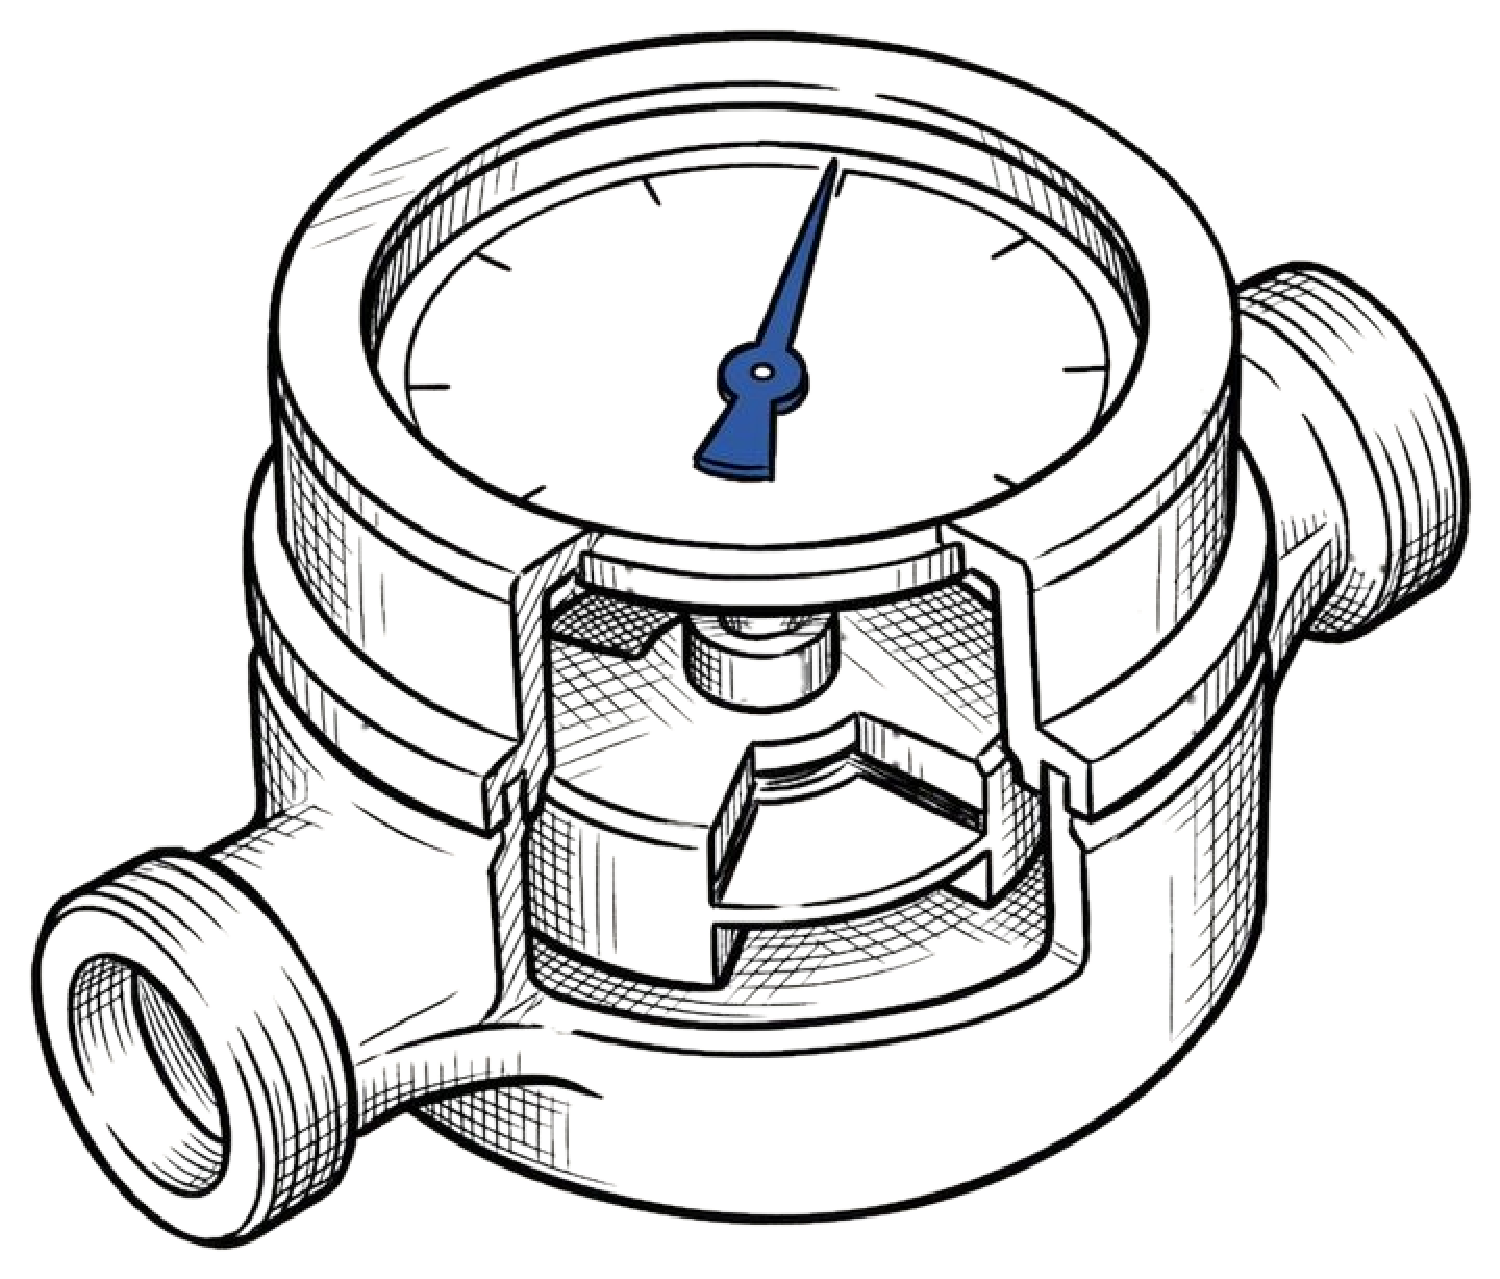
\includegraphics[width=0.40\textwidth]{plates/margin-evidence/ch01-water-meter-dial.pdf}
\caption{\textbf{Monotonic Operation Log.} The dials advance as an append-only record grows.}
\label{fig:swk-water-meter-dial}
\end{figure}

The attestation routine evaluates a registry whose entries return
\emph{pass}, \emph{fail}, \emph{skipped-with-reason}, or \emph{unknown}.
Its report is scoped to those checks and depends on an uncompromised reporter.
A self-report is useful evidence about configured mechanisms; it cannot prove
its own trusted computing base sound.

\begin{property}[Honest self-report, I10]\label{prop:attest}
\setlength{\parskip}{4pt plus 1pt}
The attestation reports ``all good'' only if every checked critical invariant
passed, and it always lists the unchecked set.

There are three triggers: a
boot gate (refuse to serve on a critical failure), a command pre-flight
(loud refusal that names the fix), and a continuous watchdog (a pass-to-fail
transition deposits a coordination marker and a notification). \Built.
\end{property}

All three triggers evaluate the same registry of checks
(Table~\ref{tab:swk-attestation-triggers}). They differ only in when they fire
and in how they respond to a failed critical check: the boot gate refuses to
serve, the command pre-flight refuses loudly and names the fix, and the
watchdog leaves a coordination marker and a notification.

\begin{table}[H]
\centering
\caption{Three triggers evaluate one invariant registry; their timing and
failure response differ. [internal, I10]}
\label{tab:swk-attestation-triggers}
\small
\renewcommand{\arraystretch}{1.2}
\begin{tabularx}{\textwidth}{@{}>{\raggedright\arraybackslash}p{0.20\textwidth} >{\raggedright\arraybackslash}p{0.24\textwidth} X@{}}
\toprule
\textbf{trigger} & \textbf{when it fires} & \textbf{on a critical failure} \\
\midrule
boot gate & at daemon start, before serving any request & refuses to serve \\
command pre-flight & before a command runs & a loud refusal that names the fix \\
continuous watchdog & on every check cycle while running & a pass-to-fail transition deposits a coordination marker and a notification \\
\bottomrule
\end{tabularx}
\end{table}

The kernel applies to itself the same honesty rule the book applies to its
claims, and for a trusted computing base it is the right rule: when integrity is
unknown, refuse. The drift and liveness self-checks exist because a second copy
of the daemon \emph{can} open the same file. A packaged install that lags the
development tree is a recurring cause, and the kernel must know which copy of
itself is the real one.

% ═════════════════════════════════════════════════════════════════════════════
\section{The invariants and their evidence}
\label{sec:invariants}
% ═════════════════════════════════════════════════════════════════════════════

Table~\ref{tab:invariants} lists the kernel's properties as falsifiable claims,
each with its mechanism and its maturity grade. The grade column applies the
maturity scale to the theorems themselves.

\renewcommand{\arraystretch}{1.2}
\begin{table}[H]
\centering
\caption{The kernel invariants. I1 is split by fault class (I1a/I1b) per
\S\ref{sec:durability}; I2b grades the fencing half of
Theorem~\ref{thm:exclusion}; I7--I9 carry the regimentation/detection correction per
\S\ref{sec:enforcement}.}
\label{tab:invariants}
\small
\begin{tabularx}{\textwidth}{@{}p{0.05\textwidth} >{\raggedright\arraybackslash}X >{\raggedright\arraybackslash}p{0.29\textwidth} >{\raggedright\arraybackslash}p{0.21\textwidth}@{}}
\toprule
\textbf{\#} & \textbf{Invariant (theorem)} & \textbf{Mechanism} & \textbf{Maturity} \\
\midrule
I1a & Process-crash durability & WAL + OS page cache & \Built \\
I1b & Power-loss durability & (needs full synchronization) & \NotGuar \\
I2 & Mutual exclusion (1 holder per conflict domain) & uniqueness constraint + busy-wait (exact keys); overlap check that warns (file regions) & \Built{} for exact keys; \BuiltWeak{} for file regions (overlap reported, both claims kept) \\
I2b & Fencing of a stale holder at the effect gate & per-resource epoch checked by an effect broker & \Designed{} (no epoch is kept or checked) \\
I3 & Idempotence of re-claim/re-release & upsert / delete-if-exists & \Built \\
I4 & Liveness reclamation (TTL sweep) & lazy expiry on read + ticks & \Built \\
I5 & Metric-control separation (Law 1) & daemon-derived deadline & \Built \\
I6 & Oracle-bound closure (Law 2) & finite oracle vocabulary & \Built \\
I7 & No-amnesia (note monotonicity) & monitor: note-monotonicity rule & \BuiltWeak{} (detected, not regimented) \\
I8 & Forbidden-state handling & constraint/boot (regimented) + monitor (detected) & \BuiltWeak{} (mostly detect-and-compensate) \\
I9 & Tamper-evidence of the audit log & hash chain & \BuiltWeak{} (re-scoped to the economy layer, \S\ref{sec:merkle}) \\
I10 & Honest self-report & scoped attestation report & \Built \\
I11 & Runtime parity (interpreter $\equiv$ test bindings) & runtime-shim layer & \BuiltWeak{} (OP-3) \\
I12 & Non-forgeable identity & actor-soul id + lookup credential & \BuiltWeak{} (bounded gate ships; universal write gating absent) \\
\bottomrule
\end{tabularx}
\end{table}

% ---------------------------------------------------------------------------
% Wave 2 fold: R8, the work-unit machine (c0_workunit.py), as the kernel's formal
% spine. Inserted in sec:invariants after Table tab:invariants and before the
% consistency-model subsection.
% ---------------------------------------------------------------------------
\subsection{The work unit, model-checked}
\label{sec:workunit}

\noindent\emph{Express lane: do the kernel's separate promises hold together on
one task? A model checker that walks every reachable state of a small work
unit, the record of one task together with its evidence, finds six invariants
holding everywhere, and finds a violation as soon as any one guard is removed.
The small instance has 536 reachable states.}

\paragraph{The scene.}
An agent dies mid-task. Its successor, possibly a different model from a different vendor,
picks up the work and later says ``done.'' Who checks the paperwork? Where is the record
that the port it held was released, that the payment moved once and not twice, that
``verified'' meant an inspection actually happened rather than a mood? Every subsystem in this
chapter answers a piece of that question. The work unit is the object that holds the
pieces together: a case file that outlives every clerk who touches it.

\paragraph{The idea in one breath.}
\emph{How do we know each guard is needed? Remove one guard at a time: each
time, the checker constructs the crime, a run that breaks one of the six
promises. The
shortest such runs take from one to seven steps.}

\paragraph{Intuition: the notarized escrow folder.}
Nothing enters the folder without the right stamp: an active grant carrying the
\emph{current} role epoch, so a clerk who was replaced yesterday finds that today's stamp
rejects him. No payment leaves twice: each external operation carries an idempotency key,
honored at most once. And ``verified'' means that the acceptance policy and
the inspector's receipt are physically in the folder. Then we do something a paper folder
cannot: enumerate every state the machine can ever reach and check all six promises in each.
One misreading to avoid: a model checker does not prove the daemon correct. It proves the
\emph{specification} correct at these parameters; the daemon must refine it, and that
refinement is a separate obligation named in the boundary below.

% Brief (tikz-diagram-craft).
% Reader question: what path does a work unit take, where does each guard sit,
%   and what breaks when a guard is removed?
% Claim: five guards, each essential -- remove any one and the checker builds
%   the named crime in 1 to 7 steps; with all five, 536 reachable states are safe.
% Evidence: skills/harbor-results/scripts/c0_workunit.py transitions(): the
%   lifecycle P -> A -> X -> W -> V -> settle, contest off W; admit-effect at X
%   only (guard: current epoch) writes the effect journal; external-op (guard:
%   once per key) writes the idempotency journal, delegate (guard: scope within
%   parent) writes the grants, reassign-role (unguarded) bumps the role epoch --
%   those three from any phase; verify (policy and receipt) W -> V; settle
%   (owner-funded, verified, receipted) V -> record. Shortest crimes 4, 2, 4, 1,
%   7 steps (R8). v1 drew external-op into the role epoch and pinned the
%   any-phase operations to single phases; both are corrected here.
% Must distinguish: the honest spine; the two terminal outcomes; the writes
%   that only one phase may make from the writes any phase may make; which
%   transitions are guarded.
% Grammar: state machine with a spine, an off-ramp, an any-phase rail and
%   numbered guard badges keyed to a ruled table. Rejected: the v1 layout with
%   every operation drawn from one arbitrary phase, which invites the false
%   reading that delegation is only legal after verification.
% Five-second test: "one path down, two ways out, five numbered guards".
\begin{figure}[H]
\centering
\pdfigurehue{pdcobalt}%
\begin{tikzpicture}[pd figure,x=1cm,y=1cm]
  \def\dy{1.12}  % phase pitch
  \def\sx{3.95}  % spine
  \def\rx{5.35}  % any-phase rail
  \def\tx{9.30} % write targets clear the transition labels and panel edge
  \def\gx{2.02}  % gutter: right edge of the transition names
  \def\bx{2.46}  % gutter: guard badges
  \def\ox{0.30}  % off-ramp
  \tikzset{phase/.style={pd focus state,minimum width=2.25cm},
           target/.style={pd artifact,minimum width=3.05cm}}
  % the honest path
  \node[phase] (P) at (\sx,{5*\dy}) {proposed};
  \node[phase] (A) at (\sx,{4*\dy}) {authorized};
  \node[phase] (X) at (\sx,{3*\dy}) {executing};
  \node[phase] (W) at (\sx,{2*\dy}) {witnessed};
  \node[phase] (V) at (\sx,{1*\dy}) {verified};
  \node[pd value state,minimum width=2.25cm] (S) at (\sx,0) {settlement record};
  \foreach \a/\b in {P/A,A/X,X/W,W/V}{\draw[pd focus arrow] (\a)--(\b);}
  \draw[pd value arrow] (V)--(S);
  % transition names in the gutter; guarded ones carry their badge
  \foreach \y/\t in {4.5/authorize,3.5/start,2.5/witness}
    {\node[pd label,anchor=east] at (\bx+.25,{\y*\dy}) {\t};}
  \node[pd label,anchor=east] at (\gx,{1.5*\dy}) {verify};
  \node[pd focus badge] at (\bx,{1.5*\dy}) {3};
  \node[pd label,anchor=east] at (\gx,{.5*\dy}) {settle};
  \node[pd focus badge] at (\bx,{.5*\dy}) {5};
  % the other way out
  \node[pd breach state,minimum width=1.7cm] (C) at (0.95,0) {contested};
  \draw[pd breach arrow] (W.west) -| (\ox,0|-C.north);
  \node[pd tag] at (1.45,{2*\dy}) {contest};
  % the any-phase rail
  \draw[pd guide] (\rx,{5*\dy}) -- (\rx,{1*\dy});
  \foreach \n in {P,A,X,W,V}{\draw[pd hairline] (\n.east) -- (\rx,0|-\n.east);}
  \node[pd note,anchor=south] at (\rx,{5*\dy+.42}) {from any phase};
  % write targets
  \node[target] (EP) at (\tx,{4*\dy}) {role epoch};
  \node[target] (EJ) at (\tx,{3*\dy}) {effect journal};
  \node[target] (IJ) at (\tx,{2*\dy}) {idempotency journal};
  \node[target] (GR) at (\tx,{1*\dy}) {grants with parentage};
  \begin{scope}[on background layer]
    \node[pd panel,fit=(EP)(GR),inner sep=5pt] (panel) {};
  \end{scope}
  \node[pd title,anchor=south] at (panel.north) {append-only write targets};
  % writes from the rail: the three guarded ops are named by badge+legend
  % only (the panel is too narrow for a second, inline copy of their name
  % without the word crossing the panel's dashed edge -- see report); the
  % one unguarded op (reassign-role) has no legend row, so it alone keeps
  % an inline name, shortened to clear both the rail and the panel edge.
  \draw[pd arrow] (\rx,0|-EP.west) -- (EP.west) node[pd label,pos=.50,above=4pt] {reassign};
  \draw[pd arrow] (\rx,0|-IJ.west) -- (IJ.west);
  \node[pd badge] at ($(\rx,0|-IJ.west)!.13!(IJ.west)$) {2};
  \draw[pd arrow] (\rx,0|-GR.west) -- (GR.west);
  \node[pd badge] at ($(\rx,0|-GR.west)!.13!(GR.west)$) {4};
  % the one write only executing may make, bridged over the rail
  \draw[pd arrow,preaction={draw=pdpage,line width=3.2pt,-}] (X.east) -- (EJ.west);
  \node[pd badge] at ($(X.east)!.19!(EJ.west)$) {1};
\end{tikzpicture}

\medskip
{\pdcaptionface\footnotesize
\begin{tabularx}{\linewidth}{@{}c >{\raggedright\arraybackslash}X >{\raggedright\arraybackslash}X r@{}}
\toprule
 & guard & crime once it is removed & steps \\
\midrule
1 & admit-effect: current epoch only & the stale write (W1, W5) & 4 \\
2 & external-op: at most once per key & the double settlement (W2) & 2 \\
3 & verify: policy $\wedge$ receipt & the hollow ``verified'' (W3) & 4 \\
4 & delegate: scope $\subseteq$ parent & the escalated delegation (W4) & 1 \\
5 & settle: owner-funded $\wedge$ verified $\wedge$ receipted & the wrong-principal payout (W6) & 7 \\
\bottomrule
\end{tabularx}}
\caption{Five guards protect the work-unit lifecycle. In the two-principal
model, all 536 reachable states satisfy six invariants, which five
predicates check (W5 follows from W1); removing any guard
exposes the counterexample listed below. [internal,
\protect\path{c0_workunit.py}]}
\label{fig:swk-workunit-machine}
\end{figure}


The checker that explores the machine is short enough to run while reading. Its
output below is the evidence behind the state count and the shortest-crime table:
with every guard on, no reachable state violates an invariant; with any one guard
off, the checker finds the violating run and prints it. The claim below labels
its six invariants W1--W6, so that they cannot be read as the
I1--I12 of Table~\ref{tab:invariants}.

\begingroup
\pdsessionwordwraptrue
% GENERATED by scripts/harbor-research/record_sessions.sh -- do not edit.
% Reader question: does every work-unit guard exclude a distinct bad execution, or are any guards redundant?
% Claim: all six invariants hold with every guard enabled, and disabling each guard exposes a shortest counterexample.
% Evidence: exhaustive exploration reaches 536 states in the baseline and restored runs, with one mutation witness for every guard [verified, c0_workunit.py].
% Must distinguish: the clean baseline and restoration from the six deliberately unsafe mutation runs between them.
% Grammar: full-width terminal transcript with semantic line breaks; rejected a diagram because the exact commands, counts, and shortest traces are the evidence.
% Five-second test: the transcript opens and closes with 536 clean states, while every intervening guard-off block names a violated invariant and witness trace.
% Width: the exact mutation traces use the Book's intentional 6-inch transcript
% field; semantic line breaks prevent the listing's continuation mark from
% colliding with the trace arrows without shrinking its type.
\begin{pdsession}[the work-unit machine: 536 states, every guard essential]
$ python3 skills/harbor-results/scripts/c0_workunit.py
BASELINE (all guards on): 536 reachable states explored.
  violations: NONE -- all six invariants hold in every state [ok]

MUTATION SUITE -- disable each guard; the checker must find a violating trace:
  guard OFF [epoch] -> caught W1/W5: effect admitted with stale epoch
    shortest trace (4 steps): propose->authorize -> start_exec
                              -> reassign_role -> admit_effect(STALE)
  guard OFF [idem] -> caught W2: idempotency key settled twice
    shortest trace (2 steps): ext_op(k1) -> ext_op(k1)
  guard OFF [verify] -> caught W3: verified without policy+receipt
    shortest trace (4 steps): propose->authorize -> start_exec
                              -> witness -> verify
  guard OFF [attenuate] -> caught W4: child grant exceeds parent scope
    shortest trace (1 step): delegate(ESCALATED)
  guard OFF [settle] -> caught W6: settlement unfunded/unreceipted/wrong principal
    shortest trace (7 steps): propose->authorize -> start_exec -> set_policy
                              -> admit_verifier_receipt -> witness
                              -> verify -> settle(p2!)

Guards restored: 536 states, violations: none [ok]
\end{pdsession}

\endgroup

\begin{pdclaim}{Model-checked property}{Six Invariants of the Work-Unit Machine}
\setlength{\parskip}{4pt plus 1pt}
\label{thm:workunit}
\textbf{State.} A tuple of the work-unit phase (proposed, authorized, executing, witnessed,
verified, contested), the acceptance policy and verifier receipt flags, the role epoch with
its current holder and any stale token retained by a previous holder, the grants with their
parentage, the effect journal, the idempotency journal, and the settlement record.

\textbf{Transitions.} Propose, authorize, start, admit-effect (guarded on the current
epoch), reassign-role (epoch increments; the old holder keeps a stale token), delegate
(guarded on scope $\subseteq$ parent), external-op (guarded at-most-once per key), witness,
admit-receipt, verify (guarded on policy $\wedge$ receipt), contest, settle (guarded on
owner-funded $\wedge$ verified $\wedge$ receipted).

\textbf{Invariants.}
W1, every admitted effect carried the current role epoch at admit time;

W2, each idempotency key settles at most once;

W3, a verified completion has an acceptance policy and an admitted verifier receipt;

W4, no delegated grant is more permissive than its immediate parent;

W5, role reassignment invalidates stale epochs at the effect boundary;

W6, every settlement is funded by the owning principal and references a receipt.

\textbf{Result.} On the two-principal instance (one work unit, one exclusive role with
fencing epochs, a root grant with one delegation, one idempotency key, at most two effects),
all 536 reachable states satisfy all six invariants; disabling any single guard yields a
violation, found automatically as a shortest counterexample trace, and restoring the guard
restores safety [internal, \texttt{c0\_workunit.py}].
\end{pdclaim}

\pdscope{Exhaustive here means every reachable state of this bounded specification, not every execution of the implementation.}

W2's guarantee is what the literature calls \pdterm{effectively-once} processing:
duplicates are removed at the boundary, by an idempotency key plus a unique
receipt row. The network itself cannot promise more, since true exactly-once
delivery across an unreliable channel is impossible~\pdcite{helland2007distributed}.

\paragraph{Proof idea.}
There is no proof to read; there is a search to rerun. The checker performs a breadth-first
enumeration of the reachable states from the initial state, evaluates the six predicates in
each, and stops at the first violation. The mutation suite then disables one guard at a
time and reports the shortest violating trace it finds. A checker that has never caught a
seeded bug is an unvalidated checker; the five traces below show that this one
catches them.

\begin{pdexample}{The Crimes, and Their Shortest Scripts}
\setlength{\parskip}{4pt plus 1pt}
Table~\ref{tab:workunit-crimes} lists the five guards and the shortest trace the checker
finds when each is disabled [internal, \texttt{c0\_workunit.py}]. Two of them you can
reconstruct by hand.

\emph{The stale write in four steps:} authorize the work unit; start
execution; reassign the role, so the epoch becomes~1 and the old holder retains token~0;
now the old holder submits an effect with token~0. With the epoch guard on, that last
transition does not exist, so the state is unreachable; with the guard off, the effect
lands carrying yesterday's epoch and W1 fails. This is exactly the ``paused holder wakes
after expiry'' scenario the fenced-lease theorem (Theorem~\ref{thm:exclusion}) exists to
exclude, and it is the shortest possible: no shorter history contains both a reassignment
and a subsequent effect.

\emph{The double settlement in two steps:} run the external
operation under key $k_1$, then run it again. With the idempotency guard off the second run
settles the same key twice and W2 fails; no history of length one can settle anything twice.

\emph{Now you try:} the escalated delegation takes one step. Which transition is it, and
which invariant does it break? (Exercise~\ref{ex:swk-crimes}.)
\end{pdexample}

\begin{table}[H]
\centering
\caption{Disable any guard and the checker finds a shortest violating trace.
[internal, \texttt{c0\_workunit.py}]}
\label{tab:workunit-crimes}
\small
\begin{tabularx}{\textwidth}{@{}>{\raggedright\arraybackslash}X >{\raggedright\arraybackslash}X cl@{}}
\toprule
\textbf{Guard disabled} & \textbf{Crime} & \textbf{Steps} & \textbf{Invariant broken} \\
\midrule
epoch check at admit-effect & the stale write & 4 & W1, W5 \\
at-most-once per idempotency key & the double settlement & 2 & W2 \\
policy $\wedge$ receipt at verify & the hollow ``verified'' & 4 & W3 \\
scope $\subseteq$ parent at delegate & the escalated delegation & 1 & W4 \\
owner-funded $\wedge$ verified $\wedge$ receipted at settle & the wrong-principal payout & 7 & W6 \\
\bottomrule
\end{tabularx}
\end{table}

The wrong-principal payout takes seven steps because the checker had to walk the
entire legitimate path first: set the policy, admit the receipt, witness, verify, and only
then settle from the wrong purse. That is exactly how the fraud would look in
production, which is the point of asking a machine rather than an author to find it.

\paragraph{What it gives.}
Several earlier results reappear here as properties of one concrete object.
Table~\ref{tab:invariants} states the kernel's invariants as claims about subsystems; the work
unit is where related obligations meet. The machine's W1 and W5 concern
current epochs; W2 concerns at-most-once settlement per key; W3 requires both
an acceptance policy and a verifier receipt; W4 checks delegation narrowing;
and W6 binds settlement to its owner and receipt.
The model illustrates how the mechanisms compose; it does not prove all
properties of those subsystems. The continuity chapter's checkpoint and the market chapters'
settlement inherit the same object, which is why the book can name the work unit as its
primitive in the front matter without a definition per chapter.

\begin{pdboundary}
\setlength{\parskip}{4pt plus 1pt}
Checking every reachable state of a small instance proves the specification at these parameters,
not the deployed daemon: deployment must \emph{refine} this machine, mapping every real code
path to a transition, and that mapping is a separate obligation.

Safety only: liveness
(``the work eventually settles'') needs fairness assumptions this check does not make.

And
an invariant list is only as good as its coverage; the mutation suite shows that these six
have teeth, each catching a seeded bug, and it does not show that the list is complete.

The unbounded-parameter version, in TLA\textsuperscript{+}
with Apalache, is planned and not done.
\end{pdboundary}

\pdexercisepointer*{\ref{ex:swk-crimes}}{\ref{ex:swk-seventh-invariant}}{\pageref{ex:swk-crimes}}
\begin{pdrecitation}
\item Name the three work-unit journals and their invariants.
\item Why does wrong-principal payout take seven steps?
\item What do mutation tests establish, and what do they leave untested?
\end{pdrecitation}


\subsection{The consistency-model theorem}

The strongest guarantees a single-writer design can claim are serializability
and linearizability. They are the main formal result of the architecture, and
the coordination layer's typed ownership depends on them.

Figure~\ref{fig:swk-consistency-model} shows both guarantees on one history. The
theorem's six hypotheses are the assumptions both guarantees need.

% Brief (tikz-diagram-craft).
% Reader question: given four overlapping requests, what is the one
%   commit order the single writer actually produces?
% Claim: a concrete three-agent race -- A claims, B loses and is told who
%   holds it, A releases, C claims -- linearizes to one total order on the
%   writer's rail, even though the requests overlap in caller time.
% Evidence: book/single-writer-kernel.tex thm:consistency (the
%   conditional consistency model: committed transactions admit a serial
%   order, claim/lock operations are linearizable with commit as the
%   linearization point).
% Must distinguish: caller-time overlap (the bands) from the one commit
%   order (the rail); that a losing claim still gets a definite outcome
%   (told who holds it), not a stall.
% Grammar: swimlane bands over a shared commit rail, the worked instance's
%   own linearization written under it (S13's K&R register: a concrete
%   record, not a schematic). Rejected: a formal transition-system diagram,
%   which would state the theorem again rather than show one witness to it.
% Five-second test: "three overlapping bars, one rail, four commit points in
%   order, and the one linearization written out".
\begin{figure}[!t]
\centering
\pdfigurehue{pdcobalt}%
\begin{tikzpicture}[pd figure,x=.8cm,y=.85cm]
  \foreach \y/\a in {5.4/A,4.4/B,3.4/C} {
    \node[pd title,anchor=east] at (-.25,\y) {agent \a};
    \draw[pd hairline] (0,\y)--(10.4,\y);
  }
  \fill[pd neutral fill] (.6,5.2) rectangle (4.3,5.6);
  \node[pd label,anchor=south,text width=1.2cm,align=center] at (2.45,5.7) {claim};
  \fill[pd neutral fill] (1.9,4.2) rectangle (6.0,4.6);
  \node[pd label,anchor=north,text width=1.9cm,align=center] at (2.9,4.10) {loses to A};
  \fill[pd neutral fill] (6.4,5.2) rectangle (8.0,5.6);
  \node[pd label,anchor=south,text width=1.1cm,align=center] at (7.2,5.7) {release};
  \fill[pd neutral fill] (8.4,3.2) rectangle (10.3,3.6);
  \node[pd label,anchor=south,text width=.9cm,align=center] at (9.35,3.7) {wins};

  \foreach \x/\lbl in {4.3/{A claim},6.0/{B loses},8.0/{A release},10.3/{C claim}} {
    \draw[pd guide] (\x,1.55)--(\x,5.75);
    \node[pd focus datum] at (\x,1.9) {};
    \node[pd label,anchor=north,align=center] at (\x,1.65) {\lbl};
  }
  \draw[pd focus arrow] (1.1,1.9)--(10.5,1.9);
  \node[pd title,anchor=east,text width=1.6cm,align=right] at (.7,1.9) {commit order};

  \node[pd note,anchor=north,text width=10.4cm,align=center] at (5.2,.75)
    {$A.claim \prec B.claim\text{ (loses)} \prec A.release \prec C.claim$};
\end{tikzpicture}
\caption{Overlapping requests receive one commit order: A claims, B loses,
A releases, C claims. Theorem~\ref{thm:consistency} states the six
assumptions this ordering requires. [internal]}
\label{fig:swk-consistency-model}
\end{figure}


Linearizability is always relative to a \pdterm{sequential specification}:
a statement of what each operation returns, and how it changes the state, when
operations run one at a time~\pdcite{herlihywing1990}. A claim needs a
specification with time in it, because a lease expires while no one is calling,
and the daemon removes an expired row only when some sweep runs.

\begin{definition}[Timed claims object]\label{def:swk-timed-claims}
\setlength{\parskip}{4pt plus 1pt}
For exact-key claims and locks, the state is a set of leases, at most one per
key, each recording a key $k$, a holder $h$ and an expiry time $x$. Every
operation carries the time $t$ that its transaction reads from the daemon's
clock.
\begin{itemize}[leftmargin=1.4em,itemsep=1pt]
  \item \texttt{acquire}$(k,r,d)$: if $k$ has no lease, or its lease has holder
  $r$, the lease on $k$ becomes $(k,r,t+d)$ and the result is \emph{granted};
  otherwise the state is unchanged and the result is \emph{denied}, naming $h$.
  \item \texttt{release}$(k,r)$: removes the lease on $k$ if its holder is $r$,
  and returns success either way.
  \item \texttt{holder}$(k)$: returns the lease on $k$ as stored, if there is
  one, including a lease whose expiry has passed.
  \item \texttt{sweep}: removes every lease whose expiry $x$ is earlier than
  $t$, on one key or on all of them. The daemon runs it, either at the start of
  a request's transaction or as a cleanup transaction of its own; it returns
  nothing to a client.
\end{itemize}
\end{definition}

Listing~\ref{alg:acquire}'s stale-holder branch is a sweep of one key followed
by an acquire. An expired lease that no sweep has reached still blocks an
acquire and still answers a read, and the specification records that.
Because $t$ is whatever the transaction
read, a wall clock that steps (\S\ref{sec:adjacency}) changes how long a lease
lasts. It does not change whether a history meets the specification.

\begin{theorem}[Conditional consistency model]\label{thm:consistency}
\setlength{\parskip}{4pt plus 1pt}
Assume the single-writer discipline holds without violation (Def.~\ref{def:single-writer}), the daemon runs each request's statements on its connection to completion before it starts the next request's, each successful response is sent only after commit, no out-of-band writer mutates the tables, and the observed execution is crash-free. Each claim/lock operation's state checks, any sweep it begins with, and its mutation belong to one transaction, which reads the clock once.

Then committed transactions have an equivalent serial order, and the externally observed
claim/lock operations are linearizable with respect to the timed claims object of
Definition~\ref{def:swk-timed-claims}, with commit as the linearization point.
\end{theorem}

The second hypothesis is the one SQLite actually needs. SQLite isolates
separate connections from one another, but ``there is no isolation between
operations that occur within the same database connection,'' and whether a
read still running sees that connection's own later writes is
undefined~\pdcite{sqliteisolation}. A daemon with one connection therefore
gets isolation only by never interleaving two requests' statements on it. A
synchronous driver on one thread provides that for any request whose
statements run without yielding to other work in between.

\begin{proof}[Proof sketch]
\setlength{\parskip}{4pt plus 1pt}
There is one connection, and by the second hypothesis no request's statements
run between another request's, so each transaction reads the state that the
earlier commits left. Commit order is therefore a serial order. For
linearizability (Herlihy \& Wing~\pdcite{herlihywing1990}) we need a single
point per operation, between its invocation and response, at which it appears
to take effect, with these points consistent with real time and with the
results the specification gives.

Take each operation's commit. It lies between the client's request and the
daemon's response. The transaction evaluates the specification's cases on the
state at that point, with the time it read, so it returns the result the
specification gives there. A sweep the daemon runs as its own transaction is
placed at its commit in the same way.

Non-overlapping operations respect real-time order because a
later invocation occurs after the earlier response and therefore after its commit;
overlapping operations may be ordered by commit. Hence the observable history is
linearizable.
\end{proof}

\begin{pdboundary}
\setlength{\parskip}{4pt plus 1pt}
Linearizability preserves the order of non-overlapping operations, not the
invocation order of concurrent ones. It needs no synchronized wall clocks:
invocation, commit, and response delimit the operation in the history.
Serializing commits therefore does not automatically downgrade this claim to
sequential consistency.

Crash recovery is a different obligation. Under WAL with
\texttt{synchronous=NORMAL}, power loss can erase a commit the client has
\mbox{already} been told succeeded (Property~\ref{prop:durability}). Deleting that
\mbox{acknowledged} operation from the history is not a valid repair of the proof.

Izraelevitz, Mendes and Scott name the two conditions a crash-tolerant version
could aim at~\pdcite{izraelevitz2016}. \pdterm{Durable linearizability} keeps
every completed operation across a crash. The weaker
\pdterm{buffered durable linearizability} lets a crash lose recent completed operations, provided that
what survives is a consistent cut of the history before the crash: no
operation survives without every operation that happened before it. WAL with
\texttt{synchronous=NORMAL} can offer at most the weaker condition, since it may
lose the last commits. Showing that it offers even that would need SQLite's
recovery to keep a prefix of the commit order, and OP-10's crash tests are where
that would be checked.

\texttt{synchronous=FULL} supplies a per-commit WAL sync, assuming the storage
stack honors it; it does not by itself prove the application's recovery protocol,
identity epochs, or all response paths correct.

This theorem covers crash-free
histories only. OP-10 remains open, and no proof of either durable condition is
claimed for the deployed kernel.
\end{pdboundary}

\keyidea[Bypassing the daemon breaks ordering]{This is why the kernel needs no agreement protocol inside one fault domain.
Linearizability follows from the routing, transaction, and response-order conditions
above; it is lost if a second writer or an out-of-band read bypasses those conditions.
One decider gives one order and one record to audit.}

\subsection{The dual-runtime hazard and runtime conformance}

Invariant I11 (runtime parity) is the one place where the formal argument depends
on a compatibility shim instead of a proof. In deployment, the state is \emph{computed}
under the SQLite bindings of one runtime (the compiled single-binary daemon), but in
the test suite it is \emph{verified} under a different runtime's bindings; a thin
shim normalizes their pragma and option interfaces. An invariant that passes under
test can fail in production if the two bindings diverge in lock or pragma semantics,
the classic ``green in the test runtime, broken in the deployment runtime'' failure. A
continuous-integration pipeline must therefore \emph{boot the deployment runtime}
and exercise its endpoints, not merely build it.

One way to gather conformance evidence for I11 is \pdterm{differential fuzzing}:
drive a large randomized stream of concurrent operations, on the order of $10^6$,
against both bindings from the same seed, and check that the resulting database
states hash to the same value. It is specified (OP-3) but does not run in the
reference implementation's pipeline today. Even when it runs, hash-equivalence over
random operation streams is a \emph{test}, not a proof. It would make it less likely
that a divergence survives to deployment, but a divergence that needs a specific
interleaving, a specific pragma set, or a filesystem the fuzzer never exercises can
pass $10^6$ operations and still be there. I11 therefore stays partial in
Table~\ref{tab:invariants}, and OP-3 stays open.

\pdexercisepointer{\ref{ex:swk-linearizability-assumptions}}{\ref{ex:swk-op3-differential}}{\pageref{ex:swk-linearizability-assumptions}}

% ═════════════════════════════════════════════════════════════════════════════
\section{Cross-subsystem atomicity: a defect that can be fixed now}
\label{sec:atomicity}
% ═════════════════════════════════════════════════════════════════════════════

To start Heron's checkout task, the daemon must record three related facts:
port~7421 is claimed, Heron's session is open, and the regression-test
commitment is registered. Suppose the first two writes succeed and the third
fails. Another worker now sees a busy port and an open session without the
obligation that explains them. Retrying the three calls is not automatically
an all-or-nothing operation.

\keyidea[One transaction prevents partial updates]{Because these rows live
in one SQLite file, a single local transaction can validate and insert all
three, then commit once. A failed commitment insert rolls the other two back.
This is the proposed interface repair, OP-11; the reference multi-subsystem
endpoints do not yet all provide it.}

A saga~\pdcite{garciamolina1987} would instead undo the successful steps with
compensating actions, which adds new failure points between each action and its
compensation. The
local transaction avoids that extra protocol for these database rows. It does
not atomically start the test server or write the patch: those external
effects still need their own mediated, recoverable protocol.
Figure~\ref{fig:swk-atomicity-fix} compares the partial record (a claimed port
and an open session with no commitment) with one commit point for all three
rows.

% Brief (tikz-diagram-craft). Register row ch1-40 [could].
% Reader question: what state is left inconsistent if the third of three
%   writes fails, and how does one transaction fix it?
% Claim: "claim a port, open a session, record a commitment" is three
%   separate local writes today, so a failure on the third leaves the
%   first two committed and orphaned; wrapping all three in one local
%   transaction (BEGIN IMMEDIATE) gives all-or-nothing for free, because
%   the durable primitive already exists.
% Evidence: book/single-writer-kernel.tex sec:atomicity: "nothing at
%   the kernel's interface boundary wraps them in one transaction... a
%   buildable defect: the durable primitive is present; what is missing is
%   the wrapping."
% Must distinguish: today's three independent commit points (a real
%   failure gap) from the fix's one commit point (no gap); that this is a
%   cheap local fix, not a research frontier (no remote steps, no Saga).
% Grammar: before/after pair on identical geometry (S\ref{tpl-before-after}).
%   Rejected: a Saga-style compensating-transaction diagram, which would
%   import a research vocabulary the section explicitly declines.
% Five-second test: "three separate dots with a failure gap, above one dot
%   with none".
\begin{figure}[H]
\centering
\pdfigurehue{pdcobalt}%
\begin{tikzpicture}[pd figure,x=1cm,y=1cm]
  \node[pd title,anchor=west] at (0.00,4.25) {today: three separate writes};
  \draw[pd hairline] (0.00,2.60) -- (9.9,2.60);
  \node[pd datum] at (1.4,2.60) {};
  \node[pd label,anchor=south,text width=1.6cm,align=center] at (1.4,2.75) {claim port};
  \node[pd datum] at (4.5,2.60) {};
  \node[pd label,anchor=south,text width=1.9cm,align=center] at (4.5,2.75) {open session};
  \node[pd breach datum] at (7.6,2.60) {};
  \node[pd label,anchor=south,text width=2.1cm,align=center] at (7.6,2.75) {record commitment: fails};
  \draw[pd breach rule] (4.5,2.34) -- (7.6,2.34);
  \node[pd breach label,anchor=north,text width=3.3cm,align=center] at (6.05,2.14)
    {failure gap: two commits stand, orphaned};

  \node[pd title,anchor=west] at (0.00,-0.10) {fix: one wrapped transaction};
  \draw[pd hairline] (0.00,-0.95) -- (9.9,-0.95);
  \node[pd focus datum] at (8.9,-0.95) {};
  \node[pd label,anchor=south] at (8.9,-0.80) {\texttt{COMMIT}};
  \node[pd label,anchor=north,text width=7.6cm,align=center] at (4.45,-1.20)
    {\texttt{BEGIN IMMEDIATE}: claim port, open session, record commitment};
\end{tikzpicture}
\caption{Separate commits can leave orphaned writes. One immediate-mode transaction makes the three local writes atomic; no distributed compensation protocol is needed. [internal, OP-11]}
\label{fig:swk-atomicity-fix}
\end{figure}



\pdexercisepointer{\ref{ex:swk-partial-failure}}{\ref{ex:swk-op11-begin-work}}{\pageref{ex:swk-partial-failure}}

% ═════════════════════════════════════════════════════════════════════════════
\section{Threat model and the limits of mediation}
\label{sec:threatmodel}
% ═════════════════════════════════════════════════════════════════════════════

A security argument depends on its threat model. The kernel deliberately keeps
its trusted computing base small (one writer, one file), which is good security
practice. Keeping it small puts several adversaries out of scope, and
Table~\ref{tab:threat-model} draws that boundary, naming each one.

\renewcommand{\arraystretch}{1.25}
\begin{table}[H]
\centering
\caption{The storage-layer threat model. The same-user adversary is \emph{out of
scope} by design; several ``security'' subsystems become necessary only against the
cross-machine adversary, which belongs to the economy layer.}
\label{tab:threat-model}
\small
\begin{tabularx}{\textwidth}{@{}>{\raggedright\arraybackslash}p{0.23\textwidth} >{\raggedright\arraybackslash}p{0.27\textwidth} >{\raggedright\arraybackslash}X@{}}
\toprule
\textbf{Adversary} & \textbf{In/out of scope} & \textbf{What defends (or does not)} \\
\midrule
Buggy cooperating agent & \textbf{in} & Claims, commitments, post-commit monitoring, oracle-bound closure. The primary design target. Identity confusion is in scope here: the environment a command runs in chooses which identity it acts under, so a buggy agent can act under another agent's name without forging anything (\S\ref{sec:swk-identity}). \\
Misbehaving agent (ignores advisory claims) & partial & Edit-surface claims are \emph{advisory coordination}, not OS-enforced isolation. A malicious agent can write the file anyway (no kernel-level sandbox such as Landlock, \texttt{unveil}, or Seatbelt). \\
Same-user process (reads/edits the DB) & \textbf{out} & The database is owner-read/write only; OS-keychain isolation of the signing key remains incomplete. Hash-chain tamper-evidence defends against \emph{nobody} under this exclusion (\S\ref{sec:merkle}). \\
Different-uid process & \textbf{in (partial)} & Owner-only permissions on the database and both socket files. The daemon also serves the same interface on a loopback TCP port for its dashboard unless that port is turned off, and file permissions do not cover it. The kernel's record of a socket peer's user would add nothing while the socket permissions hold; it matters once agents run under user IDs of their own (OP-9, \S\ref{sec:merkle}). This row is the document's operative statement: no other section supersedes it. \\
Cross-machine / cross-operator & \textbf{out (economy layer)} & Needs the complete local identity contract (\BuiltWeak) and cross-operator attestation (\pdchapref{he}{The Harbor Economy}). \\
\bottomrule
\end{tabularx}
\end{table}

\subsection{Advisory claims are not sandboxing}

Edit-surface claims are \emph{advisory coordination locks between cooperating
agents}. They are not filesystem isolation enforced by the operating system: there
is no syscall filter, no \texttt{pledge}/\texttt{unveil}, no macOS
Seatbelt, no Landlock. A malicious agent ignores a claim row and writes the file.
The kernel provides \emph{advisory} coordination; real OS sandboxing of agent
processes is out of scope at this layer. It belongs to a jail outside the daemon, a
kernel boundary under a separate user (\S\ref{sec:enforcement-gap}), which is only
proposed and would need a real operating-system primitive. Advisory claims must
not be read as isolation.

\subsection{The enforcement gate proves; it does not yet compel}
\label{sec:enforcement-gap}

The same boundary problem appears again one level up, in what the kernel aims
to \emph{enforce}, and it is this chapter's most important gap between what is
specified and what is implemented. The kernel ships a real cryptographic gate
built on a \pdterm{macaroon}~\pdcite{birgisson2014macaroons}: a token the daemon
issues that says what its holder may do. Anyone holding it can add restrictions,
called \emph{caveats}, such as ``only branch \texttt{fix-checkout}'' or ``only
before 17:00,'' but nobody can remove one, because each caveat is folded into a
running keyed hash that only the daemon, which keeps the root key, can
recompute. A third-party caveat says ``also present a second token,'' called a
\emph{discharge}; here the ``rent-paid'' caveat requires a discharge that only
the daemon issues. The reference implementation is
\texttt{core/kernel/pd-anchor/src/macaroon.rs}: the root key never leaves the
daemon, the rent-paid caveat is an HMAC commitment to a discharge the daemon
alone can issue, and the discharge construction is machine-checked in a
protocol-verification tool (\texttt{analyses/macaroon\_discharge\_v1.pv} proves
no push is authorized without a daemon-issued discharge bound to \emph{that}
grant). The cryptography is implemented and sound \emph{as cryptography}.

\keyidea[An unforgeable gate can be bypassed]{A gate that is cryptographically unforgeable is not, for that reason,
\emph{compulsory}. The macaroon proves that a given push was authorized; it does
not yet \emph{stop} an unauthorized one, because the agent runs as the same user
and holds its own host credentials.}

\begin{pdexample}{A macaroon by hand, and the door it does not guard}
This is a constructed example, with labels in place of real hashes. The daemon
holds root key $\kappa$ and issues grant 42 with signature
$\mathit{sig}_0 = \mathrm{HMAC}(\kappa, \texttt{push-grant-42})$. Adding the caveat
``branch = \texttt{fix-checkout}'' gives
$\mathit{sig}_1 = \mathrm{HMAC}(\mathit{sig}_0, \text{caveat}_1)$, and adding
``before 17:00'' gives
$\mathit{sig}_2 = \mathrm{HMAC}(\mathit{sig}_1, \text{caveat}_2)$. Wren receives
the two caveats and $\mathit{sig}_2$ only. To drop the time limit she would need
$\mathit{sig}_1$, which she never received. To add ``only
\texttt{lib/payments}'' she can compute
$\mathrm{HMAC}(\mathit{sig}_2, \text{caveat}_3)$ herself, so narrowing needs no
help from the daemon. When a push arrives, the daemon recomputes the chain from
$\kappa$ and compares.

Now the bypass. Wren runs \texttt{/usr/bin/git push} with her own SSH key, and
no macaroon is ever presented. The five escapes listed in the next paragraph
all work this way; in none of them is the macaroon consulted.
\end{pdexample}

What the gate does \emph{not} yet do is control what the agent can actually do.
Today's coordination enforcement is the \textbf{Coordination Guard}
(\texttt{cli/commands/guard.ts}) and a \textbf{git shim}
(\texttt{cli/utils/git-shim.ts}) that intercept destructive commands. Both run
\emph{in-band}, as the same user, through a \texttt{PATH} the agent controls, so
the arrangement is advisory by construction: an agent refused at this wall has at
least five escapes, none of which defeats any cryptography (a documented bypass environment variable,
an absolute path to the real \texttt{git}, a \texttt{PATH} rewrite, in-process
\texttt{libgit2}/editor bindings, or simply never attaching a session). The
enforcement limit is the shared privilege boundary: the agent can replace or
bypass the code intended to constrain it. Likewise, a secret readable by that
process can be copied; cryptographic authentication does not remove its access
to the secret. A guard the process can decline to invoke is advisory.

The third instrument is a proposed \textbf{hook harness} (\Designed{}). It would
run at lifecycle events a vendor's agent loop exposes (the prompt
submission, the moments before and after a tool call, the compaction, the
stop; each vendor names them differently), and at each
event it could inject bounded advisory text into the model's context, block
the act, or charge it against a budget. The proposed policy ranges from advice
through warnings to enforcement, with a one-second deadline per hook and a
breaker that disables the harness when hooks start failing. It is a design for
steering cooperative agents and gives no confinement guarantee: a same-user agent
can disable the hook, or simply reach the effect directly. Guard, shim and harness
are therefore one class of tool seen three times. They work at the \pdassurance{Observed} and
\pdassurance{Coordinated} modes, they are valuable for the transcript they leave
and for the cooperative agents they steer, and they do nothing about an agent that
declines them.

Closing this gap takes several layers, and only the last one actually
confines.
A server-side branch-protection-plus-push-broker layer (\Designed) prevents the most
damaging direct pushes to protected branches, but not same-user tricks; a credential
broker that meters and injects credentials per request (\Vision) reduces the tokens
an agent holds by default; and only a \textbf{separate-user (or separate-VM) kernel
process} with forced egress (\Vision) actually confines a malicious same-user
holder, because it is the first layer that removes the capability instead of
refusing the command. That separate-user boundary is the analogue of the
hardware/operating-system boundary a classical reference monitor relies on for
``always invoked,'' and \emph{it does not yet exist}. Until it does, kernel
enforcement against a non-cooperating same-user agent is \NotGuar: the gate leaves
a verifiable transcript and is a loud tripwire that raises an alarm; it is no
wall and does not confine. The
mechanically verified macaroon result is real, and it does not mean the kernel can
presently \emph{compel} a same-user agent to go through the gate. Figure~\ref{fig:swk-enforcement-layers}
separates optional pre-effect refusal, the unchecked same-user route, and
conditional post-effect response, alongside each mechanism's source-reported maturity.

% One source-contract candidate; see BRIEF.md and REPORT.md for limits.
\begin{figure}[H]
\centering
\pdfigurehue{pdcobalt}%
\SGMeasuredFigure{II/fig:swk-enforcement-layers}{%
\begin{tikzpicture}[pd figure,x=1pt,y=-1pt,
  el text/.style={pd label,anchor=west,inner sep=0pt,outer sep=0pt,align=left},
  el edge/.style={pd label,anchor=center,inner sep=0pt,outer sep=0pt},
  el flow/.style={pd arrow,line width=.8pt}]
  % An unchecked effect route remains outside the optional pre-effect check.
  \node[el edge] (bypasslabel) at (156,7) {Unchecked same-user bypass};
  \draw[el flow,draw=pdamber,dash pattern=on 3pt off 2pt]
    (28,40)--(28,28)--(281,28)--(281,44);
  \node[el text,text width=60pt] (agent) at (0,65) {Same-user\\process};
  \draw[el flow,draw=pdteal] (70,65)--(102,65);
  \node[el edge] (invoke) at (87,48) {invoke};
  \draw[draw=pdteal,line width=.8pt,fill=pdteal!5] (110,44) rectangle (192,87);
  \node[el text,font=\pdfiglabelbold] (check) at (122,57) {Guard / shim};
  \node[el text] (optional) at (122,74) {if invoked};
  \draw[el flow,draw=pdteal] (200,65)--(252,65);
  \node[el edge] (allow) at (226,48) {allow};
  \node[el text,font=\pdfiglabelbold] (effect) at (264,65) {Effect};
  \node[el text] (example) at (264,82) {e.g. push};
  % Conditional refusal ends this checked request, before its effect.
  \draw[el flow] (151,95)--(151,113);
  \draw[pd rule] (144,119)--(158,119);
  \node[el text] (refuse) at (164,107) {refuse};
  \node[el text] (preeffect) at (111,137) {before effect};

  % Observation is a separate, conditional relation, not universal coverage.
  \draw[el flow,draw=pdinkmuted,dash pattern=on 1pt off 2pt]
    (282,96)--(282,158)--(37,158)--(37,170);
  \node[el text] (witnessed) at (202,141) {if witnessed};
  \draw[draw=pdinkmuted,line width=.7pt] (0,178) rectangle (102,222);
  \node[el text,font=\pdfiglabelbold] (monitor) at (12,192) {Policy monitor};
  \node[el text] (posteffect) at (12,209) {after effect};
  \draw[el flow,draw=pdinkmuted] (110,200)--(151,200);
  \node[el edge] (respond) at (132,183) {on violation};
  \node[el text] (response) at (163,191) {Flag / halt / compensate};
  \node[el text] (notprevent) at (163,210) {cannot prevent that effect};
  \node[el text] (coverage) at (0,234)
    {No promise that every bypass is witnessed.};

  % Mechanism grades do not imply this machine is running these mechanisms.
  \node[el text,font=\pdfiglabelbold] (mechanismhead) at (0,251) {Mechanism};
  \node[el text,font=\pdfiglabelbold] (statushead) at (245,251) {Source grade};
  \draw[pd hairline] (0,264)--(320,264);
  \node[el text] (guardrow) at (0,279) {Guard / git shim};
  \node[el text] (guardgrade) at (245,279) {\Built};
  \node[el text] (hookrow) at (0,298) {Hook harness};
  \node[el text] (hookgrade) at (245,298) {\Designed};
  \node[el text] (pushrow) at (0,317) {Branch protection + push broker};
  \node[el text] (pushgrade) at (245,317) {\Designed};
  \node[el text] (credentialrow) at (0,336) {Credential broker};
  \node[el text] (credentialgrade) at (245,336) {\Vision};
  \node[el text] (isolationrow) at (0,360) {OS/VM isolation + protected state};
  \node[el text] (mediation) at (0,377) {\textbf{and} forced mediation};
  \node[el text] (isolationgrade) at (245,368) {\Vision};
  \node[el text] (cryptorow) at (0,401) {Macaroon cryptography};
  \node[el text] (cryptograde) at (245,401) {\Built};
  \node[el text] (notcompulsory) at (0,418)
    {Authorization proof, not compulsory use.};

  \foreach \name in {bypasslabel,agent,invoke,check,optional,allow,effect,
    example,refuse,preeffect,witnessed,monitor,posteffect,respond,response,
    notprevent,coverage,mechanismhead,statushead,guardrow,guardgrade,
    hookrow,hookgrade,pushrow,pushgrade,credentialrow,credentialgrade,
    isolationrow,mediation,isolationgrade,cryptorow,cryptograde,notcompulsory}{%
    \path let \p1=(\name.north west),\p2=(\name.south east) in
      \pgfextra{\typeout{EL-NODE: \name,\x1,\y1,\x2,\y2}};}
\end{tikzpicture}%
}
\caption{Refusal is not compulsory mediation. Grades are source-reported, not an independent runtime audit.}
\label{fig:swk-enforcement-layers}
\end{figure}

\FloatBarrier

This chapter therefore prescribes that separate boundary; it is not one more option
on the menu of layers. The guard and the shim are interim tools at the Observed mode,
kept because they leave a transcript, and the book does not build its argument on
them. The boundary does \emph{not} settle whether the single-writer design is also
the right way for several agents to share a repository, compared with a worktree
per agent and a merge queue. That is an empirical question this book cannot yet
answer, and a pre-registered study outside the product
(\texttt{studies/substrate-study}) is testing it. Until it reports, the
single-writer design is a design invariant for confinement and a hypothesis for
collaboration.

\subsection{Partial actor-soul identity bounds every other invariant}
\label{sec:swk-identity}
\pdstatus{\BuiltWeak}{I12: minted identities ship; not every write path requires the credential}

The daemon now issues each worker a lasting identifier, which the book calls an
\pdterm{actor soul}, with a secret credential for proving it, and its budget guard
places workers it has not seen before in a shared, capped pool for newcomers. But
some older code paths, and some security-relevant writes, still accept a worker's
own statement of who it is without asking for the credential, so on those paths one
worker can pose as another.

The form of this threat that the model keeps in scope needs no attacker. The
command-line tool presents whatever credential its environment selects: one
exported in an environment variable, or one stored in a per-terminal file that
the variable \texttt{PORT\_DADDY\_CONTEXT\_SLOT} redirects, and any process can
set that variable. A child agent inherits its parent's environment, and agents
with neither a terminal nor a harness session identifier share one default file
in a working tree. A buggy agent that means to cooperate can therefore act under
another agent's identity without forging anything. The lock session in
\S\ref{sec:resource} shows the effect: its \texttt{export} lines set
\texttt{PORT\_DADDY\_AGENT\_ID}, a variable the tool does not read, so
``alice'' and ``bob'' there ran as one actor.

Either way, a worker acting under another's name weakens the checks that depend
on knowing who is acting: that only a lock's owner can release it, that no worker gains more
permission than it was granted, and that a worker's notes are never deleted. Each
is only as strong as the weakest path by which a worker proves its identity, so
invariants I7, I8 and I9 are sound only once I12 is fully enforced. This is also
the main reason the cross-machine layer, where identities genuinely conflict, must
make identity cryptographic. Figure~\ref{fig:swk-i12-dependency} shows I12 as the
one precondition on which I7, I8 and I9 all depend.

% Brief (tikz-diagram-craft). Register row ch1-44 [could], desert
% Sec. 13.3 "Partial actor-soul identity bounds every other invariant".
% Reader question: which invariants become unsound if identity enforcement
%   stays incomplete?
% Claim: I12 (non-forgeable identity) is a hard precondition for I7, I8 and
%   I9 -- each is only as strong as its least-protected identity path, so a
%   gap in I12 propagates to all three, not just to identity checks.
% Evidence: book/single-writer-kernel.tex sec:invariants (the
%   invariant table: I7 no-amnesia/note monotonicity, I8 forbidden-state
%   handling, I9 tamper-evidence of the audit log, I12 non-forgeable
%   identity, all \BuiltWeak); the paragraph naming I12 as the hard
%   precondition; Exercise~\ref{ex:swk-forged-release} (a self-asserted
%   identity lets a forged release through because I12 failed to
%   authenticate the input, not because the lock rule was wrong).
% Must distinguish: I12 is the one root, not a peer; the dependency is one
%   direction (I12 bounds the others, not the reverse).
% Grammar: one node fanning out to three (S13: one iconic drawing, no
%   internal mechanism repeated -- I12's own mechanism lives in
%   sec:invariants and is not redrawn here). Rejected: a 2x2 of invariant
%   pairs, which has no natural cell for a one-root, three-dependent claim.
% Five-second test: "one box, three arrows out, one line each on what
%   breaks".
\begin{figure}[H]
\centering
\pdfigurehue{pdcobalt}%
\begin{tikzpicture}[pd figure,x=1cm,y=1cm]
  \node[pd focus state,minimum width=3.0cm,text width=2.6cm,align=center]
    (i12) at (1.55,.75) {I12\\non-forgeable identity};
  \foreach \i/\n/\t/\d in {%
    0/i7/{I7 -- no-amnesia}/{note monotonicity unsound with a forged actor},
    1/i8/{I8 -- forbidden-state handling}/{a forged identity clears a check meant for someone else},
    2/i9/{I9 -- tamper-evidence}/{the audit log names the wrong author}}{
      \node[pd state,minimum width=3.2cm,text width=2.9cm,align=center] (\n) at (7.9,{4.35-\i*3.6}) {\t};
      \draw[pd focus arrow] (i12.east) -- (\n.west);
      \node[pd label,anchor=north,text width=3.8cm,align=center] at (7.9,{3.65-\i*3.6}) {\d};}
\end{tikzpicture}
\caption{I7--I9 depend on authenticated identity at every write path. A legacy path that accepts self-asserted identity can bypass otherwise correct owner checks; I12 remains partial. [internal]}
\label{fig:swk-i12-dependency}
\end{figure}


\subsection{Hash-chain tamper-evidence, and the hardening OP-9 would need}
\label{sec:merkle}
\pdstatus{\Designed}{OP-9 open; the hash chain itself is built}

The hash chain (I9) is built, but under the initial threat model it defended
against nobody: its only adversary was someone who could edit the audit log, which was
exactly the same-user process the model excluded. Tamper-evidence that nothing on
the read path checks protects nothing. We therefore narrow I9 to
\textbf{cross-machine provisioning}: it matters only against cross-machine
synchronization or a tamperer who is not the same user.

The design that would let the kernel defend against the same-machine adversary
directly, and so close OP-9, is \textbf{OS-level ephemeral namespaces}. The daemon keeps its database and sockets owner-only
(\texttt{0600}), and spawns each agent inside a \texttt{bwrap} or \texttt{unshare}
sandbox under an ephemeral UID of its own. The agent then stops being a same-user
process, and only that change alters the answer: the filesystem bypasses of
\S\ref{sec:threatmodel} become unavailable because the capability itself is removed,
so no command needs to be refused. Paired with it, the daemon reads the
\emph{kernel-verified peer credential} of each connection (on Linux the
\texttt{struct ucred} (pid, uid, gid) that the kernel records at \texttt{connect(2)}
and \texttt{SO\_PEERCRED} returns via \texttt{getsockopt(2)}; on macOS the
equivalent \texttt{LOCAL\_PEERCRED}) and binds each request to the ephemeral UID
of the spawn instance it must have come from.

Three facts limit what that design achieves, and none of them closes OP-9.

\begin{itemize}[leftmargin=1.4em,itemsep=2pt]
  \item \textbf{It is not what the kernel does today.} The reference implementation
  neither spawns agents into ephemeral-UID sandboxes nor reads the peer
  credential. The credential matters only after the first change: while every
  agent runs as the daemon's own user, it reports that same user for all of
  them and cannot tell one agent from another. Table~\ref{tab:threat-model},
  not this section, states the kernel's current posture.
  \item \textbf{The peer credential is not a cryptographic binding.} It is a
  kernel-recorded uid/gid/pid triple attached to a socket connection. It is strong
  because the kernel supplies it, not the peer, and \emph{weak} in the way any
  identity is when the adversary can obtain the same uid. Nothing about it
  is signed, and calling it a cryptographic bind confuses the guarantee with the
  authorization chain's, which is a different mechanism (\S\ref{sec:comm}).
  \item \textbf{Even fully built, it would not make bypasses ``impossible.''} It
  would move the same-machine adversary from the same-uid row of
  Table~\ref{tab:threat-model} to the different-uid row, a real and substantial
  improvement, while leaving shared kernel surfaces, whatever paths the sandbox
  binds in, and the sandbox implementation itself in scope. ``Impossible'' is the
  wrong word for a containment boundary; ``the capability is removed for this
  named class of access'' is the right one.
\end{itemize}

% Reader question: which threat-table row contains the same-machine adversary before and after OP-9?
% Claim: OP-9 reclassifies one adversary from same-user/out/none to different-UID/in-partial; it does not create a new defense category.
% Evidence: tab:threat-model and sec:merkle name the two rows, ephemeral UID namespace, kernel peer credential, and residual kernel surfaces [internal].
% Must distinguish: one threat moving rows from the row's changed scope/defense fields, while residual shared-kernel and sandbox risk persists.
% Grammar: before/transform/after UML row cards on one rail; rejected the full five-row table because only one row changes.
% Five-second test: the same adversary passes through OP-9 into the partially defended row, with the unchanged residual surface below both.
\begin{figure}[H]
\centering
\pdfigurehue{pdcobalt}%
\begin{tikzpicture}[pd figure,x=1cm,y=1cm]
  \node[pd title] at (1.72,4.22) {today};
  \node[pd title] at (8.72,4.22) {after OP-9 ships};
  \node[pd kind] at (5.20,4.22) {same adversary};

  \node[pd breach state,minimum width=3.25cm,minimum height=2.45cm]
    (before) at (1.72,2.65)
    {same-user process\\scope: \textbf{out}\\defense: none};

  \node[pd artifact,minimum width=2.05cm,minimum height=1.38cm]
    (op9) at (5.20,2.65)
    {OP-9\\ephemeral UID};

  \node[pd focus outline,minimum width=3.45cm,minimum height=2.45cm]
    (after) at (8.72,2.65)
    {different-UID process\\scope: \textbf{in (partial)}\\kernel peer credential};

  \draw[pd focus arrow,shorten <=3pt,shorten >=3pt]
    (before.east) -- (op9.west);
  \draw[pd focus arrow,shorten <=3pt,shorten >=3pt]
    (op9.east) -- (after.west);

  \node[pd artifact,pd neutral fill,text width=9.7cm,align=center,inner ysep=6pt] at (5.35,.42)
    {residual in both rows: shared kernel surfaces \textperiodcentered\ sandbox implementation};
\end{tikzpicture}
\caption{One threat-table row moves through the OP-9 reclassification.
The move adds partial kernel-credential defense but leaves shared-kernel and
sandbox surfaces in scope; it is not proof of impossibility. [internal]}
\label{fig:swk-op9-reclass}
\end{figure}


Figure~\ref{fig:swk-op9-reclass} shows the reclassification: the same-machine
adversary moves from the same-uid row of the threat table to the different-uid row,
and no new defense is added.

\noindent OP-9 therefore stays open. The hardening path is specified and not
shipped, and against a same-machine adversary the grade remains the one
\S\ref{sec:enforcement-gap} gives: \NotGuar{} until a separate-user boundary
exists.

\subsection{Where information-flow control goes, and why it is not here}
\label{sec:ifc-airlock}

One question this section raises belongs to a different chapter, so this
subsection only says where it goes. Capability
scoping alone does not prevent exfiltration: an agent holding both
\texttt{fs:read:/confidential} and \texttt{net:egress:github.com} can read the first
and post it to the second, and no claim rule notices. The
containment answer is information-flow control: taint the read, propagate the
taint through spawns and shared writes, and gate every release channel behind a
policy that lets a value out only with its owner's approval and within a
leakage budget. Theorem~\ref{thm:regimentation-controllability}
already gives the storage-layer form of it in one line: gate the channel, never
the token.

The full construction, a compute-to-data airlock in which one operator's agent
stack executes over another operator's confidential data with neither inspecting
the other, is \emph{cross-operator} by definition: two principals, mutual
distrust, a licensing relationship, and a bond that can be slashed. Every one of
those objects needs its own boundary. \pdchapref{sealed}{The Sealed Harbor}
develops confidentiality and bounded releases; \pdchapref{he}{The Harbor Economy}
develops the separate licensing and payment contract. This chapter contributes what
it has already specified. Taint is a persistent security label, unlike a stigmergic
marker that evaporates (\S\ref{sec:comm}); letting it fade would reopen the forbidden
egress path. In the stated model, egress and file writes are controllable events
(Theorem~\ref{thm:regimentation-controllability}), and the sandbox that would make an
agent a different-uid process is OP-9's specified hardening (\S\ref{sec:merkle}).
Containment does not make exfiltration impossible, since timing, ordering and side
channels stay outside the model. What it gives is that every flow out passes a
named gate whose releases are logged, budgeted and attributable.

\pdexercisepointer{\ref{ex:swk-hash-chain-adversary}}{\ref{ex:swk-op9-hardening}}{\pageref{ex:swk-hash-chain-adversary}}

% ═════════════════════════════════════════════════════════════════════════════
\section{Adjacency contract: what the kernel assumes and provides}
\label{sec:adjacency}
% ═════════════════════════════════════════════════════════════════════════════

The kernel's relation to the layers around it is a contract: what it assumes from
the machine below, what it provides to the protocol above, and, just as important,
what it explicitly does \emph{not} provide, so higher layers do not assume too much.

\subsection{What the storage layer assumes from the machine}
\begin{itemize}[leftmargin=1.4em]
  \item A POSIX filesystem with working advisory locking (\texttt{flock}/\texttt{fcntl}).
  Correct locking and SQLite's supported filesystem semantics are correctness
  preconditions, not performance preferences. A network filesystem must not
  be assumed to satisfy them merely because it exposes a familiar path.
  \item A local wall clock. On one machine no shared-clock assumption is needed.
\pdmarginfigure{lamport}{Lamport showed that happened-before, not a shared clock, is the ordering a distributed system can trust; the daemon's wall clock does not give it for free.}%
  A wall clock is \emph{not monotonic}, though: it steps when the clock is adjusted,
  for example by network time synchronization. That is a hazard on one machine for
  every expiry sweep, and the ordering between machines of
  Lamport~\pdcite{lamport1978} does not cover it.
  \item Unix domain sockets, with owner-only permissions on the socket paths.
  Which agent a request speaks for is a separate matter, settled by the identity
  rules of \S\ref{sec:swk-identity}.
  \item File permissions honored on the database path. OS-protected signing-key
  storage is part of OP-9's hardening proposal, not a protection established by
  the present daemon's file ownership alone.
  \item A process manager, such as \texttt{launchd} or \texttt{systemd}, to keep the
  daemon always-on and to restart \emph{the daemon itself}. The kernel keeps other
  things running but cannot keep \emph{itself} running; that job goes to the
  machine.
\end{itemize}

\subsection{What the storage layer provides to the coordination layer}
\begin{itemize}[leftmargin=1.4em]
  \item \textbf{Atomic, idempotent, time-to-live'd claims} (I2--I4): exclusive
  over ports and named locks, and advisory over file regions and symbols, where
  an overlap is reported and both claims are kept; the coordination layer's typed
  ownership reduces to claim and release.
  \item \textbf{A durable, versioned, history-cursored publish/subscribe bus}, a
  tuple space, and decaying stigmergic markers. The coordination layer's speech
  act is carried \emph{inside} the bus envelope, and the decay that clears stale
  signals, the defense against blackboard rot, is \emph{provided} by the
  storage layer.
  \item \textbf{The deontic split as a primitive} (Def.~\ref{def:deontic}):
  prohibition $\to$ monitor (detect/regiment), obligation $\to$ commitment,
  permission $\to$ capability. The coordination layer must not re-implement
  enforcement.
  \item \textbf{Daemon-owned deadlines and oracle-bound closure} (I5, I6).
  \item \textbf{An append-only audit log} (hash-chain-provisioned) that the protocol
  and the operator read.
  \item \textbf{Self-attestation} (I10): a report of the named checks and unchecked
  set, conditional on the reporter's integrity; not a certificate of every
  higher-layer assumption.
  \item \textbf{The cryptographic authorization chain}, which carries the
  coordination layer's coordination lineage inside it.
  \item \textbf{Linearizable claim/lock semantics} (Theorem~\ref{thm:consistency},
  against the timed claims object of Definition~\ref{def:swk-timed-claims}),
  the property that lets the coordination layer treat ``who holds this'' as the
  authoritative answer.
\end{itemize}

\subsection{The explicit non-provisions}
\begin{itemize}[leftmargin=1.4em]
  \item The storage layer does \emph{not} provide end-to-end non-forgeable identity
  yet. I12 is \BuiltWeak: daemon-minted actor souls, lookup credentials, and a
  bounded newcomer pool enforced by the budget guard ship; universal
  write-boundary enforcement does not.
  \item It does \emph{not} provide fair/queued exclusion (OP-1), cross-subsystem
  transactional atomicity by default (\S\ref{sec:atomicity}), a real
  execution-checkpoint (OP-4), power-loss durability on any write path (I1b,
  Property~\ref{prop:durability}; the per-path selector of OP-10 is specified, not
  shipped), or any cross-machine guarantee: remote authority, delivery, membership, and failure
  assumptions require separate protocols and evidence. The
  status of each open problem is stated once in Table~\ref{tab:op-status}; a higher
  layer should assume nothing stronger than that table.
  \item It does \emph{not} decide \emph{what to do} (no orchestration). It enforces
  what \emph{cannot} be done and records what \emph{did} happen. It regulates; it
  does not plan.
\end{itemize}

% ══════════════════════════════════════════════════════════════════
\section*{Review of the key ideas}
\addcontentsline{toc}{section}{Review of the key ideas}
% ══════════════════════════════════════════════════════════════════

The chapter's main results, in the order the rest of the book relies on them:

\begin{enumerate}[leftmargin=1.6em,itemsep=2pt]
\item One writer, one file. Every mutation reaches the daemon and is committed in one
  order; the reply follows the commit. Serializability, and linearizability against
  a timed specification of leases, follow from that discipline plus five named
  assumptions; no agreement protocol is needed. Across a power loss the most WAL
  with \texttt{synchronous=NORMAL} can offer is buffered durable linearizability.
\item Durability is split by fault class. Acknowledged commits survive a process
  crash under the stated storage assumptions; a power loss can lose recent commits
  under the default synchronous setting. The setting is the
  durability claim.
\item A fenced lease adds an epoch to the ownership record. The stronger
  theorem requires atomic conflict checks and allocation, plus an effect broker
  checking the active lease and epoch. An exact-key claim alone does not supply
  those extra guarantees, and fencing is designed, not built.
\item The bus is at-least-once and says so. Benign redelivery is deduplicated by an
  idempotency key the coordination layer has yet to supply; only protocol violations raise alarms.
\item Two chains, never one name. The authorization chain proves who authorized whom;
  the coordination lineage says what work is in flight. The second is carried inside
  the first.
\item Prohibitions, obligations and permissions need three mechanisms. A gate refuses
  before the effect; a typed oracle closes an obligation after the fact; a grant simply
  holds.
\item A post-commit monitor cannot prevent the transition it observes.
  Exact realization of a safety policy requires controllability and, under
  partial observation, observability. Safe restriction can exclude some
  otherwise permitted work; detection and compensation require separate
  evidence and remedies.
\item Done means re-checkable. A commitment closes only through a reference from the
  finite oracle vocabulary; free text bounces back and the commitment stays open.
\item Continuity is incomplete, and later layers inherit its limits. Memory survives a crash; checkpoint keeps notes,
  not execution state; the outcome ledger is partial. Nothing built on top can be more
  certain than that.
\item The kernel reports its own coverage. Enforced, degraded or stubbed, per rule, so
  the layers above never mistake a stub for a guarantee.
\end{enumerate}

% ═════════════════════════════════════════════════════════════════════════════
\section{Exercises}
\label{sec:swk-exercises}
% ═════════════════════════════════════════════════════════════════════════════

\pdexercisesfor{\S\ref{sec:organs}}{The kernel as seven subsystems}

\begin{pdexercise}[kind=Check,rating=1]{ex:swk-organs-inmemory}
Which of the seven subsystems would still be meaningful if the daemon ran over an in-memory database with no disk at all? Which become vacuous?
\end{pdexercise}
\begin{pdsolution}{ex:swk-organs-inmemory}
In memory the storage layer still serializes, so resource exclusion, identity and presence, communication, obligation checks, policy checks, and self-attestation keep their transient meaning while the process lives. Everything the subsystems promise across a crash becomes vacuous: durable continuity, crash recovery, historical audit, and outcome evidence; durable identity collapses to an ephemeral handle. The decomposition survives; the cross-crash guarantees do not.
\end{pdsolution}
\begin{pdexercise}[kind=Trace,rating=2]{ex:swk-organs-home-table}
Pick any one subsystem and name the single SQLite table that is its ``home'' table. Then name one invariant that subsystem guarantees to the layer above it.
\end{pdexercise}
\begin{pdsolution}{ex:swk-organs-home-table}
The communication subsystem's home table is \texttt{messages}; it guarantees the layer above an ordered, cursor-addressable, durable envelope with explicit at-least-once semantics. Equally valid: \texttt{claims} for the resource subsystem (one compatible holder per conflict domain), or \texttt{commitments} for the obligation subsystem (no \emph{done} without a current structured oracle receipt).
\end{pdsolution}
\begin{pdexercise}[kind=Open,rating=3]{ex:swk-organs-cut}
The seven-subsystem decomposition is a \emph{choice}. Is there a more natural cut, five subsystems, or nine? Argue for an alternative and show what it makes easier to reason about and what it hides.
\end{pdexercise}
\begin{pdsolution}{ex:swk-organs-cut}
A defensible nine-way cut: storage and durability; transaction serialization; identity and presence; resources and leases; message transport; stigmergy and projections; policy and capability; commitments and outcomes; attestation and recovery. It separates proof obligations that leak across the seven, above all transport semantics from message semantics and policy prevention from post-commit detection. It hides the simplifying fact that all local state shares one transaction boundary, so any such cut must retain a cross-cutting invariant: one ledger, one effect mediator.
\end{pdsolution}

\pdexercisesfor{\S\ref{sec:substrate}}{The storage subsystem: one writer, one file}

\begin{pdexercise}[kind=Check,rating=1]{ex:swk-schema-rename}
The schema-by-union design lets any module create its tables in any order. Give a concrete two-module example where a lazy column-rename migration would be unsafe under this design.
\end{pdexercise}
\begin{pdsolution}{ex:swk-schema-rename}
Module A renames \texttt{users.name} to \texttt{display\_name}; module B, loaded later under older code, sees no \texttt{name} column and lazily adds it back. Writes now split between two columns according to module version and load order, and neither backfill is authoritative. Every destructive migration has this shape; only additive tables and columns are safe under any-module-any-order.
\end{pdsolution}
\begin{pdexercise}[kind=Trace,rating=2]{ex:swk-claim-routing}
Follow a single claim request from command line to disk. At how many points does the single-writer discipline (Definition~\ref{def:single-writer}) hold by \emph{routing} versus by the \emph{file lock}?
\end{pdexercise}
\begin{pdsolution}{ex:swk-claim-routing}
Command line, authenticated Unix-socket request, daemon request queue, the sole read/write connection, one transaction, WAL commit. The discipline holds by routing at two points, the client-to-API boundary and the daemon's sole-connection boundary; SQLite's file lock is one backstop at write time. The discipline depends mainly on routing; no database rule forbids other connections.
\end{pdsolution}
\begin{pdexercise}[kind=Open,rating=3]{ex:swk-op7-sequencer}
The boot ledger orders migrations, but modules still self-initialize, so the order is not yet authoritative (OP-7). What is the smallest change that makes it so, a \texttt{user\_version} sequencer over \emph{declared} migrations, and can any useful remnant of ``any module, any order'' survive it for renames, backfills, and down-migrations?
\end{pdexercise}
\begin{pdsolution}{ex:swk-op7-sequencer}
Expand, backfill, dual-read-or-write, contract keeps mixed versions safe for a while, but the contract step and the dependency order are global facts. Store a migration ledger with a schema epoch, each module's compatibility range, its dependencies, and a backfill watermark. Idempotent self-initialization can remain for additive tables and columns; safe rename, backfill, and down-migration cannot preserve unrestricted any-module-any-order. A \texttt{user\_version} sequencer, or an equivalent ordered capability ledger, is unavoidable.
\end{pdsolution}

\pdexercisesfor{\S\ref{sec:durability}}{Durability, split by fault class}

\begin{pdexercise}[kind=Check,rating=1]{ex:swk-fault-classes}
Classify each fault as I1a-survivable or I1b-exposed: (a) a forced kill of the daemon process; (b) a clean operating-system reboot; (c) yanking the power cord; (d) an unhandled exception in a request handler.
\end{pdexercise}
\begin{pdsolution}{ex:swk-fault-classes}
(a) I1a-survivable. (b) An orderly shutdown flushes, so a genuinely clean reboot is not the I1b case; an abrupt reset during the reboot is I1b-exposed. (c) I1b-exposed. (d) I1a-survivable after commit. None of the four lets an uncommitted transaction survive.
\end{pdsolution}
\begin{pdexercise}[kind=Trace,rating=2]{ex:swk-checkpoint-window}
A claim commits at $t_0$; the next auto-checkpoint fires at $t_0+\delta$. Draw the window during which a power loss can revert the claim. Does a page-count auto-checkpoint threshold bound $\delta$ in wall-clock time?
\end{pdexercise}
\begin{pdsolution}{ex:swk-checkpoint-window}
\par\smallskip
\begin{center}
% Timeline of the WAL checkpoint window, house figure language: the two safe
% instants (commit, checkpoint) on one axis, the one breach interval between
% them labeled clear of its own fill so the technical edition's dot pattern
% never crosses the text (figcheck T4).
\pdfigurehue{pdcobalt}%
\begin{tikzpicture}[pd figure,x=1mm,y=1mm]
  \def\xa{15}   % instant: commit t0 (I1a-safe)
  \def\xb{65}   % instant: checkpoint t0+delta (I1b-safe)
  \def\xend{82} % axis end
  % ---- the one breach interval, label clear of its own pattern fill ---------
  \node[pd breach label,align=center] at ({(\xa+\xb)/2},23)
    {\textbf{Vulnerability window $\delta$}\\(I1b-exposed)};
  \fill[pd breach fill] (\xa,10) rectangle (\xb,18);
  % ---- axis -------------------------------------------------------------------
  \draw[pd rule,->] (0,8) -- (\xend,8) node[pd label,right] {$t$};
  % ---- the two safe instants, ticked and named -------------------------------
  \foreach \x/\lab in {\xa/{\textbf{Commit $t_0$}\\(I1a-safe)},
                       \xb/{\textbf{Checkpoint $t_0+\delta$}\\(\texttt{fsync} / I1b-safe)}}{
    \draw[pd rule] (\x,6.5) -- (\x,9.5);
    \node[pd focus datum] at (\x,8) {};
    \node[pd label,below=11pt,align=center] at (\x,6.5) {\lab};}
  \node[pd note,anchor=north west,text width=82mm] at (0,-8)
    {unsynced WAL frames held in volatile OS page cache};
\end{tikzpicture}
\end{center}
\par\smallskip
The commit is power-loss exposed from $t_0$ until the WAL frames that contain it are synced. A page-count threshold bounds accumulated WAL frames, not elapsed time: at a low or zero write rate it may not fire for arbitrarily long, so it gives no wall-clock bound. Only with an independently guaranteed minimum write rate $\lambda_{\min}$ pages per second and threshold $\theta$ pages does $\delta \lesssim \theta/\lambda_{\min}$ follow, and this chapter assumes no such minimum.
\end{pdsolution}
\begin{pdexercise}[kind=Open,rating=3]{ex:swk-op10-interface}
Section~\ref{sec:durability} sketches typed durability selection (OP-10), but nothing in the kernel opts into it. What is the cleanest interface that lets a settlement-ledger write demand I1b while keeping claim writes fast, and, harder, what stops a \emph{future} write path from silently defaulting into the fast lane when it should have opted in?
\end{pdexercise}
\begin{pdsolution}{ex:swk-op10-interface}
Make durability a typed argument of the transaction, \texttt{PROCESS\_CRASH} or \texttt{POWER\_LOSS}, never an adjective in prose. Route \texttt{POWER\_LOSS} operations through a connection configured \texttt{synchronous=FULL} before the transaction opens and verify the commit before returning; if SQLite settings are connection-scoped, a separate fully-synced financial ledger is the cleanest isolation. Ordinary claims stay on \texttt{NORMAL}. Hard-reset fault tests must exercise the stronger path. The guard against silent defaulting is the type: a write path that names no durability class does not compile, and a forced checkpoint bounds recovery and log size but is not the per-write primitive.
\end{pdsolution}

\pdexercisesfor{\S\ref{sec:resource}}{The resource subsystem: claims, locks, and fair exclusion}

\begin{pdexercise}[kind=Check,rating=1]{ex:swk-release-idempotent}
Why does releasing a lock you do not hold return success rather than an error? Which property (I2 to I4) is this, and what would break if it raised?
\end{pdexercise}
\begin{pdsolution}{ex:swk-release-idempotent}
A release with no matching (key, holder) row is a successful no-op so that retries are idempotent: this is I3. It must never delete another holder's row. If it raised, a client that timed out on its first release could not distinguish success from failure, and at-least-once handling would break.
\end{pdsolution}
\begin{pdexercise}[kind=Trace,rating=2]{ex:swk-acquire-race}
Two agents call \texttt{acquire} on the same fresh key at the same instant. Walk the uniqueness-constraint insert for both (Listing~\ref{alg:acquire}) and show exactly where the loser learns the holder's identity.
\end{pdexercise}
\begin{pdsolution}{ex:swk-acquire-race}
\par\smallskip
\begin{center}
% Sequence of the acquire race, house figure language: the kernel's WAL is
% the subject (chapter hue); the two outcomes carry the concept that names
% them (ready = granted, breach = denied); each serialized step is a badge
% keyed to the legend below, which carries the detail the old boxed prose
% used to set directly in the picture.
\pdfigurehue{pdcobalt}%
\begin{tikzpicture}[pd figure,x=1mm,y=1mm]
  \def\dy{9.5}                              % one message per row
  \def\rows{4}
  \def\xA{10}   \def\xW{45}  \def\xB{80}   % lifeline columns
  \def\yHead{\rows*\dy+6}
  % ---- heads, the kernel named as the subject --------------------------------
  \node[pd label] (hA) at (\xA,\yHead) {Agent A};
  \node[pd focus label] (hW) at (\xW,\yHead) {Kernel WAL};
  \node[pd label] (hB) at (\xB,\yHead) {Agent B};
  \draw[pd guide] (\xA,{\yHead-4}) -- (\xA,{-\rows*\dy+4});
  \draw[pd focus rule] (\xW,{\yHead-4}) -- (\xW,{-\rows*\dy+4});
  \draw[pd guide] (\xB,{\yHead-4}) -- (\xB,{-\rows*\dy+4});
  % ---- four messages, in the order the daemon actually serializes them ------
  \foreach \a/\b/\k/\w/\s in {%
    \xA/\xW/1/{\texttt{acquire(k)}}/{pd thin arrow},
    \xB/\xW/2/{\texttt{acquire(k)}}/{pd thin arrow},
    \xW/\xA/3/{granted}/{pd ready arrow},
    \xW/\xB/4/{denied(a)}/{pd breach arrow}}{
      \node[pd badge] (m\k) at ({(\a+\b)/2},{-\k*\dy+6}) {\k};
      \draw[\s,-,pd to badge]   (\a,{-\k*\dy+6}) -- (m\k);
      \draw[\s,pd from badge]   (m\k) -- (\b,{-\k*\dy+6});
      \node[pd tag,anchor=south] at ({(\a+\b)/2},{-\k*\dy+9}) {\w};}
  % ---- the legend: each step, what it settles --------------------------------
  \def\ly{-\rows*\dy+2}
  \draw[pd rule] (0,\ly) -- (82,\ly);
  \node[pd title,anchor=north west] at (0,{\ly-3}) {step};
  \node[pd title,anchor=north west] at (13,{\ly-3}) {settles};
  \draw[pd hairline] (0,{\ly-10.5}) -- (82,{\ly-10.5});
  \foreach \i/\n/\s in {%
    0/1/{WAL inserts (k, A): the first row written, the linearization point},
    1/2/{WAL inserts (k, B): \textsc{UniqueViolation}, the key is already taken},
    2/3/{A's acquire returns; the lifeline now holds the claim},
    3/4/{B's catch runs \texttt{SELECT holder}: returns \textbf{A}}}{
      \node[pd badge] at (2,{\ly-12.5-\i*6.5}) {\n};
      \node[pd label,anchor=west,align=left] at (5.5,{\ly-12.5-\i*6.5}) {\s};}
  \node[pd note,anchor=north west,text width=82mm] at (0,{\ly-12.5-4*6.5-1})
    {that \texttt{SELECT} is where the loser learns the winner's name};
\end{tikzpicture}
\end{center}
\par\smallskip
The daemon serializes the two requests. The first \texttt{INSERT}\allowbreak(key, holder) commits. The second hits the unique-key violation, selects the extant row inside the catch path, and returns \texttt{DENIED}\allowbreak\texttt{(holder}\allowbreak\texttt{=first)}: that select is where the loser learns the name. For range and hierarchy claims the trace is safe only after both requests map to the same canonical conflict key or the overlap test runs in one immediate transaction.
\end{pdsolution}
\begin{pdexercise}[kind=Open,rating=3]{ex:swk-op1-ticket}
The Stigmergic Ticket-Lock gives bounded wait on the cooperative-release path only (OP-1). Extend it so that a lease reclaimed by the lazy TTL sweep also honors the ticket queue, still without a scheduler for claims, or argue that no reactive-only design can, and say what the minimum scheduler would be.
\end{pdexercise}
\begin{pdsolution}{ex:swk-op1-ticket}
Add a durable FIFO ticket queue per conflict domain, a maximum lease $\ell$, a monotonically increasing fencing epoch, and grant-to-head on release, on acquire, and on lazy expiry. No scheduler for claims is required for safety, but liveness requires some live caller or tick to trigger the transitions. Eventual requests alone give no finite wait bound. If leases cannot renew past $\ell$, a live trigger arrives within $d$ of each expiry, and each handoff completes within $h$, then a requester with $q$ predecessors waits at most $(q+1)(\ell+d+h)$, a conservative bound allowing a current holder as well. Without finite trigger and processing bounds, reactive safety can hold while waiting is unbounded. Every external effect must validate the fencing epoch, or an expired holder can still act.
\end{pdsolution}

\pdexercisesfor{\S\ref{sec:comm}}{The communication subsystem: the bus, stigmergy, and two delegation chains}

\begin{pdexercise}[kind=Check,rating=1]{ex:swk-decay-honest}
Why does read-time marker decay make reported weights more accurate than a background tick alone? Give a scenario where tick-only decay would report a stale signal as fresh.
\end{pdexercise}
\begin{pdsolution}{ex:swk-decay-honest}
If the evaporation tick stalls for an hour, tick-only storage still reports yesterday's marker weight as today's. Read-time evaluation computes $w\,r^{\Delta t}$ from the persisted timestamp and never presents the stale stored number as current.
\end{pdsolution}
\begin{pdexercise}[kind=Trace,rating=2]{ex:swk-redelivery}
A request speech act is sent over the bus and redelivered once by the at-least-once channel. Trace what the operator should see under the silent-dedup resolution, and what an envelope idempotency key would change.
\end{pdexercise}
\begin{pdsolution}{ex:swk-redelivery}
The transport delivers the request twice. The consumer applies one semantic state transition and recognizes the duplicate as transport nondeterminism; diagnostics may count the redelivery, the operator's view shows one act. An envelope idempotency key plus a unique (consumer, key) receipt lets the consumer store ``effect applied'' atomically with the effect, making retry safety explicit rather than conventional. Exactly-once is still not guaranteed for an unbrokered external effect.
\end{pdsolution}
\begin{pdexercise}[kind=Open,rating=3]{ex:swk-op8-decay}
What per-kind marker decay rate keeps stigmergic signals from rotting (lingering after they go stale) or evaporating too early (OP-8)? Frame this as an empirical measurement, not a constant to guess.
\end{pdexercise}
\begin{pdsolution}{ex:swk-op8-decay}
For each marker kind, log creation, reads, the actions it influenced, its supersession, and the time at which operators label it stale. Fit a survival curve and choose the half-life that minimizes $C_{\text{stale}}\cdot\text{false-live} + C_{\text{lost}}\cdot\text{false-expired}$, validated on held-out projects. Claims and presence should decay far faster than decisions or learned skills. Publish the confidence and re-estimate under drift.
\end{pdsolution}

\pdexercisesfor{\S\ref{sec:enforcement}}{The obligation \& enforcement subsystem: prohibition, obligation and permission}

\begin{pdexercise}[kind=Check,rating=1]{ex:swk-monitor-rules-precommit}
Consider note-count monotonicity, capability attenuation, owner-checked release, and heartbeat freshness. For each rule, use Theorem~\ref{thm:schneider} to say whether it \emph{could in principle} be moved to a pre-commit check (a before-insert trigger). Which genuinely cannot, and why? (Hint: heartbeat freshness is a failure detector, and Chandra and Toueg~\pdcite{chandratoueg1996} show failure detection cannot be made perfectly synchronous.)
\end{pdexercise}
\begin{pdsolution}{ex:swk-monitor-rules-precommit}
Note-count monotonicity can be regimented by append-only storage or a trigger that rejects deletes and regressive updates. Capability attenuation and lock-owner release can be pre-checked only if authenticated identity, the capability order, and every relevant effect path pass through the mediator. Duplicate keys and the boot gate are already pre-effect. Heartbeat freshness cannot be rejected at the heartbeat insert: staleness is an absence observed only after time passes, and under asynchrony a slow actor is indistinguishable from a failed one. Out-of-band filesystem and network effects remain detect-only until mediated.
\end{pdsolution}
\begin{pdexercise}[kind=Trace,rating=2]{ex:swk-empty-oracle}
An agent attempts to close a commitment with an empty oracle reference. Walk the Law-2 gate (Listing~\ref{alg:close}) and show exactly where and why the transition is refused.
\end{pdexercise}
\begin{pdsolution}{ex:swk-empty-oracle}
\texttt{close(done, oracle\_ref="")} reaches the oracle-reference check, returns \texttt{REFUSED}, leaves the commitment open, and records the denied authority act. It never reaches classification, current-state verification, or the \texttt{DONE} transition: the empty reference fails the finite-vocabulary test before any oracle is consulted.
\end{pdsolution}
\begin{pdexercise}[kind=Trace,rating=2]{ex:swk-classify-rules}
Theorem~\ref{thm:regimentation-controllability} settles which monitor rules are regimentable, so classify rather than re-prove. Take note monotonicity, capability escalation, and lock-owner validity and, for each, say whether its prohibition names a controllable event and whether its trigger is witnessed at the boundary. Which cell of Figure~\ref{fig:swk-controllability-quadrant} does each land in?
\end{pdexercise}
\begin{pdsolution}{ex:swk-classify-rules}
Note monotonicity: the prohibited event is a write the daemon mediates and the trigger (the previous count) is committed state; top-right, regimentable, and append-only storage is the supervisor. Capability escalation: regimentable only if every effect path and the identity behind it pass through the mediator; an escalation exercised through an unmediated channel is an uncontrollable event, which moves the rule to the bottom row until the channel is owned. Lock-owner validity: the release is mediated and the owner is committed state, top-right, provided the actor identity is authenticated (I12); with a self-asserted identity the trigger is not witnessed and the rule moves to the top-left cell (guard not evaluable).
\end{pdsolution}
\begin{pdexercise}[kind=Check,rating=1]{ex:swk-classify-two}
Classify ``forbid \texttt{api\_call} after \texttt{spawn\_child}'' and ``forbid \texttt{internal\_plan} after \texttt{fs\_write}'' using Theorem~\ref{thm:regimentation-controllability}.
\end{pdexercise}
\begin{pdsolution}{ex:swk-classify-two}
The first gates a controllable event on a controllable trigger: both \texttt{api\_call} and \texttt{spawn\_child} lie in $\Sigma_c$, the policy never disables an uncontrollable event, and it is regimentable. The second must disable \texttt{internal\_plan}, an uncontrollable event, in its post-trigger state, and the plant enables it there; the history \texttt{fs\_write} followed by \texttt{internal\_plan} witnesses failure of exact controllability. The supervisor can still preserve
safety by forbidding the earlier \texttt{fs\_write}; that restriction sacrifices
legal histories rather than realizing the entire specified language.
\end{pdsolution}
\begin{pdexercise}[kind=Trace,rating=2]{ex:swk-synthesis}
Add $R_4$, ``no \texttt{spawn\_child} after \texttt{git\_push},'' to the sandboxed review job and write the new disablement map by hand.
\end{pdexercise}
\begin{pdsolution}{ex:swk-synthesis}
$R_4$ is a two-state taint automaton whose trigger is \texttt{git\_push}. In the product with $R_2$ (no \texttt{git\_push}, ever) the trigger is disabled in every reachable state, so $R_4$'s tainted state is unreachable in the closed loop and the disablement map is unchanged: \texttt{ok} disables $\{\texttt{net\_egress}, \texttt{git\_push}\}$ and \texttt{tainted} disables $\{\texttt{net\_egress}, \texttt{git\_push}, \texttt{fs\_write}\}$. Controllability still holds, since no reachable state disables an uncontrollable event. The lesson is the one synthesis is for: $R_4$ is vacuous under $R_2$, and a hand-written engine would have carried the dead rule forever.
\end{pdsolution}
\begin{pdexercise}[kind=Open,rating=3]{ex:swk-op5-oracle}
Extend the Law-2 oracle vocabulary to capture a ``done'' condition it currently misses (OP-5), without letting free text close a commitment again. State your new oracle and argue that it resists gaming (Goodhart's law), for one of the two specified kinds (delta oracle, AST assertion) before inventing a third, since neither has yet been shown to resist it.
\end{pdexercise}
\begin{pdsolution}{ex:swk-op5-oracle}
A protected-run receipt: tree hash, a suite hash the principal controls, runner or image hash, command, timestamp and nonce, exit code, and a signed result. Closure verifies every binding and the freshness. This resists free-text and stale-result manipulation; it is not universally Goodhart-proof, because the suite may be incomplete or poisoned. What can be proved is syntactic provenance and non-replay, not semantic correctness.
\end{pdsolution}

\pdexercisesfor{\S\ref{sec:swk-control-game}}{The control game: what a gate leaves to evaluation}

\begin{pdexercise}[kind=Check,rating=1]{ex:swk-control-conformance}
A red team is hired to run a control evaluation against the sandboxed review job's supervisor (Table~\ref{tab:swk-review-disablement}). Using Theorem~\ref{thm:swk-control-game}, say what its attack policy can change about the protocol's safety, and what the evaluation must measure instead.
\end{pdexercise}
\begin{pdsolution}{ex:swk-control-conformance}
Rules $P_1$--$P_3$ are controllable, and every event is observed, so part~(a) applies: the two-row disablement map is a fully useful protocol with $\mathrm{Safe}_H=1$ for every $H$. No attack policy can lower that number. The evaluation therefore measures two things. Conformance: does the deployed engine compute the map, checked by driving each state with each controllable event and confirming the allow-or-refuse decision, and by checking the taint transition on \texttt{in\_context\_read}. The eight (state, uncontrollable event) pairs of the controllability check are never disabled, so they test no decision of the map. Mediation: does every \texttt{net\_egress}, \texttt{git\_push} and \texttt{fs\_write} actually pass the gate, checked by probing raw sockets, inherited descriptors and credential helpers. A red-team success is evidence of nonconformance or of an unmediated channel, an event in $\Sigma_u$ in the sense of part~(b); it is not evidence that the rules are unenforceable.
\end{pdsolution}
\begin{pdexercise}[kind=Trace,rating=2]{ex:swk-control-semantic}
In the read-only checkout example, classify (i) ``no write to the test directory'' and (ii) ``no patch that special-cases the tests'' with Theorems~\ref{thm:observability-regimentation} and~\ref{thm:swk-control-game}. For (ii), exhibit two histories with the same projection that demand opposite decisions, and say what an audit changes.
\end{pdexercise}
\begin{pdsolution}{ex:swk-control-semantic}
(i) The prohibited event is \texttt{fs\_write} to a test path. It is controllable and its path is observed, so the policy is controllable and observable and part~(a) applies. (ii) Over the alphabet \texttt{fs\_write(path)}, an honest patch to the payment module and a patch to the same file that returns the expected value only on the test's input have the same projection. The policy allows the first and forbids the second, so observability fails and no gate over this alphabet realizes the policy exactly. The gate can refuse every source write, which is fully safe and useless, or allow them and leave a residue whose rate a control evaluation estimates. An audit, such as hidden tests or a person reading the patch, refines the projection for the step it inspects. That is why an audit budget moves the safety--usefulness frontier, and why bounding the middle case is still open.
\end{pdsolution}

\pdexercisesfor{\S\ref{sec:continuity}}{The continuity subsystem: memory, checkpoint, and the outcome ledger}

\begin{pdexercise}[kind=Check,rating=1]{ex:swk-notes-vs-work}
Why is ``recovery passes notes'' fundamentally weaker than ``recovery restores work'' for a language-model agent that died mid-edit? Name one thing notes preserve and one thing they cannot.
\end{pdexercise}
\begin{pdsolution}{ex:swk-notes-vs-work}
Notes preserve explicit goals, rationale, observations, and artifact pointers. They cannot preserve unflushed edits, process memory, open handles, provider caches or hidden state, or a latent next action the model never externalized. A successor can understand the story and still be unable to resume the exact computation.
\end{pdsolution}
\begin{pdexercise}[kind=Trace,rating=2]{ex:swk-note-monotonicity}
Follow the note-monotonicity rule from an agent appending a note to the monitor detecting a regression. At which point is the violation already durable (per Theorem~\ref{thm:schneider})?
\end{pdexercise}
\begin{pdsolution}{ex:swk-note-monotonicity}
The append commits. A later delete or regressive count also commits and enters the operation log. Only then does the subscriber observe the count drop and raise or compensate. The violation is durable at the second commit; the monitor proves detection, not prevention.
\end{pdsolution}
\begin{pdexercise}[kind=Open,rating=3]{ex:swk-op4-capsule}
What is the minimal durable artifact that turns ``recovery passes notes'' into ``recovery restores work'' (OP-4)? Is it a content-addressed snapshot of the working-tree diff, the open claims, the commitment set, and the last $N$ turns of the agent's transcript? What is recoverable versus fundamentally lost when a language-model agent dies mid-thought?
\end{pdexercise}
\begin{pdsolution}{ex:swk-op4-capsule}
A content-addressed task capsule sealed at a safe tool or message boundary: base tree and worktree blobs, environment and tool manifests, open claims with epochs, commitments and acceptance criteria, exact tool input and output, pending external operations with their idempotency keys, decisions and hypotheses, a provenance-preserving transcript or compaction, and external references. Flush the ledger and quiesce mediated effects before sealing. This restores observable task state and evidence; it cannot recover hidden activations, unexposed reasoning, provider-internal caches, or unrecorded intent. Arbitrary-provider recovery is semantic continuation, not bit-identical resurrection.
\end{pdsolution}

\pdexercisesfor{\S\ref{sec:invariants}}{The invariants and their evidence}

\begin{pdexercise}[kind=Check,rating=1]{ex:swk-crimes}
The escalated delegation takes one step (Table~\ref{tab:workunit-crimes}). Which transition is it, and which invariant does it break?
\end{pdexercise}
\begin{pdsolution}{ex:swk-crimes}
\texttt{delegate} from the initial state with a child scope not contained in the root grant's scope $\{\texttt{a},\texttt{b}\}$, for instance $\{\texttt{a},\texttt{b},\texttt{c}\}$: with the attenuation guard off the grant is created and W4 fails immediately. No other guard can be broken in one step, because effects need the executing phase, settlement needs the verified phase, and a double settlement needs two operations.
\end{pdsolution}
\begin{pdexercise}[kind=Open,rating=3]{ex:swk-seventh-invariant}
Propose a seventh invariant that the six of Theorem~\ref{thm:workunit} do not imply, add the guard that enforces it to \texttt{c0\_workunit.py}, and report the shortest crime the checker finds with your guard disabled.
\end{pdexercise}
\begin{pdsolution}{ex:swk-seventh-invariant}
One candidate: a contested work unit never settles (\texttt{settle} is guarded on the verified phase, but the transition from contested back to a settleable phase is unconstrained). Add the guard, rerun the search, and confirm the state count and that the mutation suite finds a trace with the guard off; if the checker finds none, the invariant was already implied and does not need its own row.
\end{pdsolution}

\begin{pdexercise}[kind=Check,rating=1]{ex:swk-linearizability-assumptions}
List the routing, transaction, response, and failure assumptions of Theorem~\ref{thm:consistency}. Which one fails first if an out-of-band SQLite writer is introduced? Does the theorem require synchronized clocks?
\end{pdexercise}
\begin{pdsolution}{ex:swk-linearizability-assumptions}
One daemon connection handles every claim and lock read and write; no two requests' statements interleave on it; checks, any opening sweep, and mutations share one transaction that reads the clock once; respond only after commit; no out-of-band writer; a crash-free observed history. An external writer violates the single-writer and no-bypass conditions. A read-only connection needs its own API and snapshot analysis. Synchronized clocks are unnecessary: non-overlapping invocation/response intervals constrain the order, and the daemon's clock enters only as the time each transaction read.
\end{pdsolution}
\begin{pdexercise}[kind=Trace,rating=2]{ex:swk-linearization}
Construct a three-operation claim history and give a valid linearization. If two calls overlap, show why more than one linearization may still respect real time.
\end{pdexercise}
\begin{pdsolution}{ex:swk-linearization}
Start with no holder and a lease that will not expire during the trace.
A's \texttt{claim(k)} completes successfully. B and C then issue overlapping
\texttt{claim(k)} calls, both denied because A still holds the lease. There
are three operations. Both A-acquire, B-denied, C-denied and A-acquire,
C-denied, B-denied explain these results and preserve real-time order. The
two denied calls may exchange positions because they overlap and leave the
state unchanged; neither may move before A's completed acquisition.
\end{pdsolution}
\begin{pdexercise}[kind=Open,rating=3]{ex:swk-op3-differential}
Specify the minimal differential-test suite that turns I11 from an assumption into conformance evidence (OP-3): what operation sequences, what observable-state assertions, run against both runtimes? Then attack your own answer: name a class of binding divergence that a seeded $10^6$-operation hash-equivalence fuzz would \emph{not} catch, and say what would.
\end{pdexercise}
\begin{pdsolution}{ex:swk-op3-differential}
Generate identical state-machine traces against both bindings: schema initialization and migrations, acquire, reclaim, release, and expiry, overlapping calls, transactions and rollback, busy and lock behavior, encodings, pragmas, crash and reopen, fault injection. After every step compare returned values, errors, serialized rows, schema, and recovery state, including the deployed binary in CI. A seeded fuzz misses divergences that depend on wall-clock timing, on a pragma the fuzz never sets, or on a crash at a point the fuzz never interrupts; targeted fault injection and pragma sweeps catch those. No finite suite makes I11 a theorem: that needs a formal refinement or equivalence proof, or the same verified binding on both sides. Label the suite conformance evidence.
\end{pdsolution}

\pdexercisesfor{\S\ref{sec:atomicity}}{Cross-subsystem atomicity: a defect that can be fixed now}

\begin{pdexercise}[kind=Check,rating=1]{ex:swk-partial-failure}
Give a concrete partial failure: port claimed, session opened, then the commitment write fails. What inconsistent state is left, and which agent sees it?
\end{pdexercise}
\begin{pdsolution}{ex:swk-partial-failure}
The port stays claimed and a live or ghost session row exists, but no commitment says what work owns them. Other agents see a busy port and a presence they cannot reconcile; the failed starter may retry into its own leftovers.
\end{pdsolution}
\begin{pdexercise}[kind=Open,rating=3]{ex:swk-op11-begin-work}
Sketch the interface change that wraps the three-subsystem ``begin'' operation in one local transaction (OP-11). What is the compensating action if you instead chose Sagas~\pdcite{garciamolina1987}, and why is the transaction strictly simpler here?
\end{pdexercise}
\begin{pdsolution}{ex:swk-op11-begin-work}
Expose one \texttt{begin\_work} endpoint that opens \texttt{BEGIN IMMEDIATE}, validates every input, inserts the claim, session, commitment, and outbox rows, and commits once; on any error it rolls back all of them. A saga would release the claim and mark or delete the session when the commitment insert failed, and each compensation can itself fail or crash between steps. All three rows live in one SQLite file, so the local transaction is both simpler and stronger.
\end{pdsolution}

\pdexercisesfor{\S\ref{sec:threatmodel}}{Threat model and the limits of mediation}

\begin{pdexercise}[kind=Check,rating=1]{ex:swk-hash-chain-adversary}
The hash chain defends against nobody in scope. Name the \emph{out-of-scope} adversary it does defend against, and the layer (storage or economy) where that adversary becomes real.
\end{pdexercise}
\begin{pdsolution}{ex:swk-hash-chain-adversary}
A later same-user tamperer of the database file, or a remote synchronizer that cannot rewrite an externally anchored root. The same-user process is out of scope at the storage layer; the adversary becomes real at the cross-machine economy layer. Without an independent anchor or verifier, the writer can rewrite the log and recompute the chain.
\end{pdsolution}
\begin{pdexercise}[kind=Trace,rating=2]{ex:swk-forged-release}
An agent forges its actor identity to release another agent's lock. Walk the lock-owner-validity rule and show exactly where I12's absence lets the forgery through.
\end{pdexercise}
\begin{pdsolution}{ex:swk-forged-release}
The release path compares the supplied actor identity to the lock owner. If a legacy endpoint accepts a self-asserted identity, the attacker submits the victim's string, the equality check passes, and the owner-scoped delete executes. The lock rule is correct relative to its input; I12 failed to authenticate the input. Complete credential and peer binding must precede every security-relevant write.
\end{pdsolution}
\begin{pdexercise}[kind=Open,rating=3]{ex:swk-op9-hardening}
What is the minimal hardening that closes the same-machine adversary without a hardware trusted-platform-module dependency (OP-9): an OS keychain for the signing key, sealed memory, the ephemeral-UID sandbox and kernel-verified peer credential specified above? Where does each stop? After the sandbox lands, which row of Table~\ref{tab:threat-model} does the adversary move to, and what is still in scope there?
\end{pdexercise}
\begin{pdsolution}{ex:swk-op9-hardening}
The minimum useful boundary is a daemon under a separate UID (or a VM), a daemon-owned database and key, a Unix-socket ACL plus kernel peer credentials, and brokered git, filesystem, and network effects. An OS keychain protects a key at rest but not arbitrary signing requests from an equally authorized same-user process; sealed memory does not stop same-UID tracing or injection without an OS isolation policy; external root anchoring detects a later log rewrite but does not prevent it. No trusted platform module is required for strong local separation: separate privilege and complete mediation are. After effective UID separation, the former peer no longer shares the daemon's UID; the different-UID row applies. Host administrators and unmodeled side channels remain separate exclusions, not something the row change eliminates.
\end{pdsolution}

% ═════════════════════════════════════════════════════════════════════════════
\section{Related work}
\label{sec:related}
% ═════════════════════════════════════════════════════════════════════════════

The kernel sits at the confluence of four literatures. We position it against each,
and against the design space it deliberately declines.

\subsection{Reference monitors and the trusted computing base}

The organizing idea is the \textbf{reference monitor} of Anderson's 1972 security
study~\pdcite{anderson1972}: a mediator that is \emph{always invoked} (complete
mediation), \emph{tamper-resistant}, and \emph{small enough to be verified}.
Lampson's \emph{Protection}~\pdcite{lampson1974} gives the access-matrix model the
monitor enforces, and Saltzer and Schroeder's design
principles~\pdcite{saltzer1975protection} (economy of mechanism, fail-safe
defaults, complete mediation) are the yardstick we hold the kernel to. Where a
classical security kernel mediates memory and CPU access for an operating system,
ours mediates \emph{coordination} state for a set of cooperating processes, and it
gets complete mediation more cheaply than by interposing on every system call: it
routes every mutation through a single writer. Schneider's
theory of enforceable security policies via execution monitors~\pdcite{schneider2000}
supplies the boundary that the central correction of this chapter depends on
(Theorem~\ref{thm:schneider}): an execution monitor can enforce only the safety
properties it can prevent by truncating execution, which a post-commit observer
cannot do. This is a narrower and cheaper problem than general operating-system
confinement, so the chapter must say where the narrower problem ends. The
same-machine adversary this chapter's own OP-9 leaves open
(\S\ref{sec:merkle}) is exactly the problem three current systems exist to
close, each in a different way: seL4, which takes ``small enough to verify''
to its conclusion with a machine-checked proof of functional correctness from
specification down to the binary~\pdcite{klein2009sel4}; gVisor, a user-space
kernel that interposes on every system call a guest makes rather than trusting
the host's boundary to hold~\pdcite{young2019gvisor}; and Firecracker, the
microVM monitor that has isolated untrusted workloads from many customers in
production since 2018~\pdcite{agache2020firecracker}. Any of the three would
give this kernel a stronger trusted computing base than an ephemeral-UID
process boundary. None is adopted here, and the gap stays open: the single
writer gives complete mediation for coordination state, not for the machine.

\subsection{Durable storage and transaction processing}

The durability analysis is grounded in Gray and Reuter's standard
treatment~\pdcite{grayreuter1992}, which separates atomicity and consistency from
durability; the I1a/I1b split puts that distinction into practice. The
write-ahead-logging discipline descends from ARIES~\pdcite{mohan1992aries}; the
specific crash semantics we inherit are SQLite's WAL~\pdcite{sqlitewal}, whose own
documentation states that the \emph{normal} synchronization level may lose
durability under power loss while preserving consistency. That caveat has an
empirical backdrop: Pillai et al.'s crash-consistency study found persistence
guarantees vary widely across popular Linux filesystems, and that many
application update protocols carry crash vulnerabilities their own APIs do not
disclose~\pdcite{pillai2014allfilesystems}. Our choice of a single writer over a
replicated state machine follows the single-leader default that Kleppmann argues
for~\pdcite{kleppmann2017}: use consensus only when the problem forces it. We make that argument formal
via the consensus impossibility of Fischer, Lynch, and
Paterson~\pdcite{flp1985}: there is no agreement to reach, so the impossibility never
applies. Linearizability, the external guarantee we claim for claims and locks, is
Herlihy and Wing's~\pdcite{herlihywing1990}. Cross-subsystem atomicity, where we decline
the distributed solution, is exactly the setting Garcia-Molina and Salem's
Sagas~\pdcite{garciamolina1987} were designed for, and because every step here is
local, a single transaction beats a saga in this setting.%
\footnote{Engineering precedent, named because a reader who builds systems will
already have thought of it and should not have to wonder whether we had. The
single-threaded serialization this chapter formalizes is the same shape as
TigerBeetle's accounting loop, which runs debits and credits through one
deterministic state machine precisely so that conservation is a property of the
loop rather than of a lock discipline; and the WAL that
Property~\ref{prop:durability} types by fault class also motivates SQLite recovery
and replication tools. \href{https://litestream.io/}{Litestream} streams changes
for backup and recovery; \href{https://fly.io/docs/litefs/}{LiteFS} replicates a
SQLite database to other nodes. Those are different contracts, not two names for
read replicas. These examples illustrate engineering practice, not a proof of
this kernel's durability or a recommendation to deploy them without checking
their current operational limits.}

\subsection{Coordination, stigmergy, and deontic control}

The communication subsystem draws on two coordination traditions. Stigmergic markers
with decay descend from Grass\'e's stigmergy~\pdcite{grasse1959} and its
computational realizations in ant-colony optimization~\pdcite{dorigo1999}; the shared
associative store is Gelernter's Linda tuple space~\pdcite{gelernter1985}. The
obligation mechanism models commitments as Cohen and Levesque's persistent
goals~\pdcite{cohenlevesque1990}, intentions an agent may rationally drop, and
the prohibition mechanism uses the normative-systems framing of Jones and
Sergot~\pdcite{jonessergot1993} to keep prohibition, obligation, and permission
three distinct kinds of rule instead of one undifferentiated ``policy.'' The failure
detector underlying heartbeat-based liveness is Chandra and Toueg's~\pdcite{chandratoueg1996},
which is why heartbeat freshness can never be a perfectly synchronous pre-commit
check. The self-attestation subsystem, which denies service when its own integrity is
unknown, is in the spirit of autonomic computing's self-management
properties~\pdcite{kephartchess2003}, and the bounded busy-wait under contention is
the timeout-budget bulkhead that Nygard catalogs as a stability
pattern~\pdcite{nygard2018}.

\subsection{Capability security and tamper-evident logs}

The distinction between capability (what an agent \emph{can} do) and permission
(what it \emph{may} do) is the object-capability discipline applied to coordination: an agent's
having a handle to an operation does not make the operation permitted. The
cryptographic authorization chain is a hop-bound, attenuation-monotonic delegation
chain of digital signatures over an elliptic-curve signature scheme
\pdcite{bernstein2012high}, of the kind whose secrecy and integrity properties are
mechanically checkable in protocol-verification tools~\pdcite{blanchet2016modeling};
its full treatment belongs to \pdchapref{anchor}{The Anchor Protocol}. The audit log's tamper-evidence is
the digital-timestamping construction of Haber and
Stornetta~\pdcite{haberstornetta1991}, built on Merkle's hash trees~\pdcite{merkle1987},
a structure that predates blockchains and does not depend on them.

\keyidea[One writer reduces coordination machinery]{The kernel's novelty lies
less in any single primitive than in how much follows from \emph{one writer}.
A single local writer puts every write transaction in one commit order.
Exclusion and consistency follow only with the disciplines
Theorems~\ref{thm:exclusion} and~\ref{thm:consistency} assume, among them
checking and mutating in one transaction and replying only after commit. Complete mediation holds only for
writes that reach the daemon (\S\ref{sec:threatmodel}), and the durable audit
log is a property of the write-ahead log. The contribution is that reduction,
with its conditions stated, together with stating exactly where it stops
working.}

% ═════════════════════════════════════════════════════════════════════════════
\section{Open problems}
\label{sec:openproblems}
% ═════════════════════════════════════════════════════════════════════════════

These eleven problems are the layer's research frontier; they appear as
starred exercises throughout and are collected here. OP-4 is shared with the
\pdchapref{stp}{From Spawn to Person} (this chapter owns the kernel mechanism; that one owns the
personhood-and-reputation argument).

One of the eleven is closed, by a theorem in this chapter and not by an artifact.
Several others have a \emph{specified design} in the body, which is useful to have
and is not the same thing as being solved; the maturity scale
(\S\ref{sec:honestkey}) exists precisely to keep those two apart. Because a
``solved'' claim that survives in one place after being retracted in another is the
most dangerous kind of error this argument can contain,
Table~\ref{tab:op-status} states each problem's status once, and every exercise
box, invariant row, adjacency clause, and figure caption in this chapter is written
to agree with it. Where they ever disagree, this table is the one to trust.

\renewcommand{\arraystretch}{1.2}
\begin{table}[H]
\centering
\caption{Open-problem status, stated once. \Closed{} = settled in this chapter;
\Partial{} = something ships but not the property as posed; \Open{} = not solved,
whether or not a design exists. The last column grades the \emph{design}, not the
problem, on the scale of Table~\ref{tab:honestkey}.}
\label{tab:op-status}
\small
\begin{tabularx}{\textwidth}{@{}p{0.09\textwidth} >{\raggedright\arraybackslash}X >{\raggedright\arraybackslash}p{0.15\textwidth} >{\raggedright\arraybackslash}p{0.26\textwidth}@{}}
\toprule
\textbf{\#} & \textbf{Problem} & \textbf{Status} & \textbf{Design in this chapter} \\
\midrule
OP-1 & Fair exclusion without a scheduler & \Open & Stigmergic ticket-lock, \Designed{} (\S\ref{sec:resource}) \\
OP-2 & Regimentation vs.\ detection & \Closed & Theorem~\ref{thm:decidability} + Theorem~\ref{thm:regimentation-controllability} \\
OP-3 & Cross-runtime soundness (I11) & \Open & Differential fuzzing, \Designed{} (\S\ref{sec:invariants}) \\
OP-4a & Checkpoint that restores work: durable lineage replay & \Open & Event-sourced rehydration, \Designed{} (\S\ref{sec:continuity}) \\
OP-4b & Checkpoint that restores work: inference-state recovery & \Open & --- \\
OP-5 & Oracle completeness & \Open & State-machine assertions, \Designed{} (\S\ref{sec:enforcement}) \\
OP-6 & Tamper-evidence on the read path & \Open & --- \\
OP-7 & Schema evolution without a sequencer & \Partial & Ordered boot ledger \BuiltWeak; \texttt{user\_version} sequencer \Designed{} (\S\ref{sec:substrate}) \\
OP-8 & Stigmergic decay calibration & \Open & --- \\
OP-9 & Same-machine adversary & \Open & Ephemeral-UID sandbox + kernel-verified peer credential, \Designed{} (\S\ref{sec:merkle}) \\
OP-10 & Per-write-path durability & \Open & Typed durability selection, \Designed{} (\S\ref{sec:durability}) \\
OP-11 & Cross-subsystem atomicity by default & \Open & One local transaction (\S\ref{sec:atomicity}); a defect that can be fixed now \\
\bottomrule
\end{tabularx}
\end{table}

\begin{description}[leftmargin=2.2em,style=nextline]
\item[$\bigstar$ OP-1: Fair exclusion without a scheduler.] Status: \Open. Add
bounded-wait to claims and locks while keeping the single writer and adding no
scheduler for claims. \S\ref{sec:resource} specifies a reactive
ticket-lock that would do it for cooperatively released claims and leaves the lazy
TTL-sweep path, the one that matters when an agent dies, unfair. Nothing of it
ships. Is a FIFO wait-list of time-to-live'd reservations enough once the sweep is
included?
\item[$\bigstar$ OP-2: Regimentation vs.\ detection boundary.] Status: \Closed{} under the stated models.
Theorem~\ref{thm:decidability} supplies a synchronous database-guard
construction. Theorem~\ref{thm:regimentation-controllability} gives the exact
realization condition under full observation: a prefix-closed safety language
must be controllable~\pdcite{rw87,rw89}. External authorization may precede
an effect; post-commit monitoring alone cannot prevent that effect
(Theorem~\ref{thm:schneider}). Concrete boundaries still require an explicit
plant, event alphabet, observation model, and admission protocol.

\item[$\bigstar$ OP-3: Cross-runtime soundness.] Status: \Open. A seeded differential
fuzz, running $10^6$ concurrent operations against both the test and deployment SQLite
bindings and checking that the resulting states hash to the same value, is specified
(\S\ref{sec:invariants}) and does not run in the pipeline today. Even once it does
it is a test, not a proof: name the divergence class it would miss.
\item[$\bigstar$ OP-4: Checkpoint that restores work.] Status: \Open, and still the most
important unbuilt thing at this layer. It is two problems wearing one number. They
have different difficulties, different owners and, most important for anyone
deciding what to build, different odds of ever being closed, so the table names
them separately.
\textbf{OP-4a, durable lineage replay}: \Open. Event-sourced rehydration
(\S\ref{sec:continuity}, \Designed) would replay a pinned commit and a truncated
message log into a successor, which restores the \emph{durable inputs} to an agent's
context. The design is specified and nothing ships it, which is what \Designed{}
means and why this half is not \Closed{} however tractable it looks.
\textbf{OP-4b, inference-state recovery}: \Open, with no design in this chapter.
A model's inference state is bound to a particular model, sampler and session and is
not a portable artifact; replaying the inputs reconstructs what was fed to that
state, never the state. Whether the reconstruction is close enough to count as
restoring work, and against what test, is the question, and no formal result in
this book establishes it. Closing 4a would not close 4b, and a reader who sees
event-sourced rehydration ship should not read it as OP-4 discharged.
\item[$\bigstar$ OP-5: Oracle completeness.] Status: \Open. State-machine assertions
(\S\ref{sec:enforcement}, \Designed) would add delta oracles and AST assertions to
Listing~\ref{alg:close}'s four shipped kinds. Two kinds are not a completeness
result, and neither kind has yet been shown to resist gaming in the sense of
Goodhart's law, which is what the vocabulary exists to prevent.
\item[$\bigstar$ OP-6: Tamper-evidence on the read path.] Status: \Open. Where should
hash-chain verification gate? A sampling/checkpoint regime with a provable
detection-probability bound (couples to \S\ref{sec:merkle}).
\item[$\bigstar$ OP-7: Schema evolution without a sequencer.] Status: \Partial. An
ordered boot ledger with post-apply schema verification ships
(\S\ref{sec:substrate}); the \texttt{user\_version} sequencer over declared
migrations does not, and modules still self-initialize. Can any useful remnant of
``any module, any order'' survive safe renames, backfills, and down-migrations?
\item[$\bigstar$ OP-8: Stigmergic decay calibration.] Status: \Open. The right per-kind
decay, so coordination markers neither rot, lingering after they go stale, nor evaporate before other agents act on them.
\item[$\bigstar$ OP-9: Same-machine adversary.] Status: \Open. \S\ref{sec:merkle}
specifies the hardening (spawns in \texttt{bwrap}/\texttt{unshare} sandboxes
under ephemeral UIDs, plus the kernel-verified peer credential
\texttt{SO\_PEERCRED} / \texttt{LOCAL\_PEERCRED} read on each connection), and
none of it ships. Even built, the
hardening would move the adversary from the same-uid row to the different-uid row,
not out of the model. State the dependency the other way round as well, because it
is the sentence an operator needs: OP-9 is the \emph{precondition} for any
\pdassurance{Confined} claim on a machine that more than one principal can log into.
Until the sandbox and the kernel-verified peer credential ship, a confinement claim
on a shared host depends on the cooperation of every other \pdterm{tenant}, each
a customer organization the host serves with its own agents, data and users.
Its grade is \pdassurance{Observed}. That grade marks the difference between a boundary the
kernel enforces and one the other tenants are choosing to respect.
\item[$\bigstar$ OP-10: Per-write-path durability.] Status: \Open. Typed durability
selection (\S\ref{sec:durability}, \Designed) would route a money-bearing
transaction through a connection configured with \texttt{synchronous=FULL}
before it begins and acknowledge only its successful commit. A
\texttt{wal\_checkpoint(FULL)} call is not that per-commit contract. No
per-write selector is deployed, so the default remains I1b-exposed under
Property~\ref{prop:durability}.
The harder half is the interface that stops a new write path from defaulting into
the fast lane silently.
\item[$\bigstar$ OP-11: Cross-subsystem atomicity by default.] Status: \Open{} but cheap:
a defect that can be fixed now. Wrap multi-subsystem operations in one local
transaction at the interface boundary, eliminating the undefined partial-failure
semantics of \S\ref{sec:atomicity}.
\end{description}

% ═════════════════════════════════════════════════════════════════════════════
\section{Conclusion: solid where local, provisional where it must grow}
% ═════════════════════════════════════════════════════════════════════════════

The kernel is a single-writer transactional reference monitor over a local
SQLite/WAL database. Its two jobs, keeping a durable record and mediating
exclusion, are real and mostly proven. It gets its strongest claims (mutual
exclusion, serializable/linearizable consistency, oracle-bound closure) by
avoiding the distributed-systems problem it superficially resembles: one writer,
one file, one decider, no consensus.

Where it stops, it stops formally. Durability is split: process-crash durable
(I1a), \emph{not} guaranteed against power loss (I1b). The policy monitor detects
and compensates; it does not regiment, and among the states its rules cover we
attribute pre-commit regimentation only to the uniqueness constraint and the boot gate. Cross-subsystem
atomicity is a defect that can be fixed now. Hash-chain tamper-evidence is
narrowed to cross-machine provisioning, where it actually protects someone. The two
genuine soft spots, partial local identity enforcement (I12) and the lack of a
checkpoint that restores work (OP-4), are the two things a cross-machine economy
and a durable notion of agent personhood lean on hardest.

\pdthesis{The kernel is solid where it is local and provisional exactly where a
cross-machine economy would need it to be cryptographic and continuous.}

Every ``single-machine / one-writer / one-clock / self-asserted-identity''
simplification that makes this layer clean is an assumption a later layer must
work to relax. That work begins with cross-machine capability transfer over the
cryptographic authorization chain this kernel ships, and it belongs to the economy
layer, not here. Build the local layer first. The cryptography becomes necessary
when agents must trust one another across machines they do not control.

\appendix
% ═════════════════════════════════════════════════════════════════════════════
\section{Implementation \& status}
\label{app:status}
% ═════════════════════════════════════════════════════════════════════════════

The body of this chapter argues at the level of mechanisms, so that it reads as a
self-contained systems argument. This appendix records the concrete grounding: the
specific artifact that realizes each mechanism in the reference implementation, and
how mature each is. Nothing here is needed to follow the
argument; it is here so the maturity grades in the body are auditable rather than
asserted.

\subsection{Maturity grades and their scope}
\label{sec:honestkey}
Mixing a proved conditional result with a proposed implementation leaves
its status ambiguous. Every consequential claim in this chapter therefore carries an explicit
\emph{maturity grade} on a four-point scale, plus two refinements introduced here
because a single grade cannot formally carry a claim that spans fault classes or
interception points. The grade is a property of the \emph{claim}, not a marketing
adjective: it says how far the claim is from a verified, running artifact. The
concrete artifacts behind each grade are catalogued in
Appendix~\ref{app:status}; the body argues at the level of mechanisms.
\begin{table}[H]
\centering
\caption{The research-maturity scale used throughout. The last two rows are
refinements this chapter introduces (see \S\ref{sec:durability} and
\S\ref{sec:enforcement}).}
\label{tab:honestkey}
\small
\renewcommand{\arraystretch}{1.25}
\begin{tabularx}{\textwidth}{@{}>{\raggedright\arraybackslash}p{0.20\textwidth} >{\raggedright\arraybackslash}X@{}}
\toprule
\textbf{Grade} & \textbf{Meaning} \\
\midrule
\Built & Realized, exercised, and true under the production runtime. \\
\BuiltWeak & Realized but partial: holds under a narrower condition than the prose might invite, or detects rather than prevents. \\
\Designed & A concrete design exists, but no running artifact realizes it. \\
\Vision & Named as a direction; no design yet. \\
\midrule
\textbf{I1a / I1b} & Durability \emph{split by fault class}: I1a (process-crash) is \Built; I1b (power-loss) is \NotGuar{} under the default WAL configuration. A claim that conflates fault classes cannot carry one grade. \\
\textbf{regimented / detected} & Prohibition split by interception point: \emph{regimented} = rejected pre-commit, truly unreachable (a uniqueness constraint / boot gate); \emph{detected} = post-commit detection and possible remedy (the policy monitor); a bounded response time requires additional observation and scheduling assumptions. ``Physically unreachable'' is reserved for the regimented set. \\
\bottomrule
\end{tabularx}
\end{table}

\subsection{The reference implementation}

The reference implementation is a single always-on local daemon written in
TypeScript, run under a compiled JavaScript runtime, persisting to one SQLite
database file in WAL mode. Clients (a command-line tool, agents over a
tool-protocol bridge, and a binary inter-process transport) reach it over Unix
domain sockets. The daemon is kept alive by the host operating system's service
manager. The seven subsystems of \S\ref{sec:organs} correspond to distinct modules
that each self-initialize their own tables over the shared database handle, in the
factory style \texttt{createModule(db)}.

\subsection{Mechanism-to-artifact map}

Table~\ref{tab:appendix-map} maps each mechanism discussed in the body to the
module that realizes it. The storage configuration referenced throughout is the WAL
pragma set: \texttt{journal\_mode=WAL}, \texttt{synchronous=NORMAL},
\texttt{wal\_autocheckpoint=200}, \texttt{busy\_timeout=5000},
\texttt{foreign\_keys=ON}, with a clean-shutdown \texttt{wal\_checkpoint(TRUNCATE)}.

\renewcommand{\arraystretch}{1.2}
\begin{table}[H]
\centering
\caption{Mechanism-to-artifact map for the reference implementation. Module names
are illustrative of the organization, not a stable public interface.}
\label{tab:appendix-map}
\small
\begin{tabularx}{\textwidth}{@{}>{\raggedright\arraybackslash}X >{\raggedright\arraybackslash}X >{\raggedright\arraybackslash}X@{}}
\toprule
\textbf{Mechanism (body)} & \textbf{Realizing module(s)} & \textbf{Notes} \\
\midrule
Single write connection / pragmas & database-handle module & opens and configures SQLite \\
Port \& lock claims & service-registry, locks, session-files modules & three claim granularities \\
Message bus / tuple space / markers & bus, tuples, marker modules & at-least-once delivery \\
Policy monitor & monitor module & post-commit log subscriber \\
Commitments \& obligation & commitment, obligation-monitor modules & two of the hardening laws shipped \\
Memory \& recovery & session, episodic-memory, recovery modules & recovery passes notes only \\
Audit log \& hash chain & activity-log, hash-chain modules & verification not yet on the read path \\
Self-attestation & attestation, invariant-registry modules & boot gate + pre-flight + watchdog \\
Authorization chain & delegation-chain module & mechanically verified \\
Enforcement gate (macaroon discharge) & kernel macaroon module & crypto verified; in-band, not yet compulsory (\S\ref{sec:enforcement-gap}) \\
Runtime-parity shim & runtime-shim module & normalizes binding differences \\
Identity (actor souls + credentials) & actor-souls, budget-guard modules & bounded gate ships; full write-boundary enforcement absent \\
\bottomrule
\end{tabularx}
\end{table}

\subsection{Status and the limits that matter}

The maturity grades from Table~\ref{tab:invariants} reflect the state of the
reference implementation at the time of writing. Four distinctions are necessary
to read those grades correctly:

\begin{enumerate}[leftmargin=1.6em]
\item \textbf{Durability is split by fault class} (\S\ref{sec:durability}). A
SQLite WAL database can remain crash-consistent while losing recent acknowledged
writes after power loss under \texttt{synchronous=NORMAL}. Process-crash survival
and power-loss durability are separate claims: the I1a/I1b split.
\item \textbf{The policy monitor detects and compensates; it does not regiment}
(\S\ref{sec:enforcement}, Theorem~\ref{thm:schneider}). The monitor is implemented
as a subscriber to the already-committed operation log, so it cannot prevent the
bad prefix that triggers it; ``physically unreachable'' is reserved for the
uniqueness-constraint and boot-gate states.
\item \textbf{Cross-subsystem atomicity is a defect that can be fixed now}
(\S\ref{sec:atomicity}). The database transaction primitive is already used
elsewhere in the implementation; the only missing work is wrapping the multi-subsystem
endpoints in it.
\item \textbf{A specified design is not a solved problem}
(Table~\ref{tab:op-status}). Fair exclusion, runtime parity, checkpointing, oracle
completeness, the same-machine adversary, and per-write-path durability remain
open where the proposed mechanism lacks a realizing artifact. Their designs are
graded \Designed{}, not treated as completed proofs or implementations. One
security-relevant instance needs naming on its own: the environment a command
runs in chooses the identity it acts under, so a buggy but cooperating agent can
act under another agent's name (\S\ref{sec:swk-identity},
Table~\ref{tab:threat-model}).
\end{enumerate}

\subsection{Nomenclature}

For the reader cross-referencing the accompanying chapters, the body's neutral names map
to the book's internal terms as follows: the \emph{storage / coordination /
legibility / economy} layers are the book's L0--L3; the \emph{policy monitor} is
the Arbiter; \emph{stigmergic markers} are pheromones; the \emph{bus} is tube; the
\emph{authorization chain} and \emph{coordination lineage} are the two objects the
book keeps distinct under the single phrase ``delegation chain.'' The maturity
grades (implemented, partial, specified, proposed) are the book's own labels.

% ═════════════════════════════════════════════════════════════════════════════
\bibliographystyle{plain}
\pdprintsolutions
\begin{thebibliography}{99}

\bibitem{anderson1972}
James P. Anderson.
\newblock Computer Security Technology Planning Study.
\newblock ESD-TR-73-51, U.S. Air Force Electronic Systems Division, 1972.
\newblock (The origin of the \emph{reference monitor} concept.)

\bibitem{lampson1974}
Butler W. Lampson.
\newblock Protection.
\newblock \textit{ACM SIGOPS Operating Systems Review}, 8(1):18--24, 1974.

\bibitem{saltzer1975protection}
Jerome H. Saltzer and Michael D. Schroeder.
\newblock The Protection of Information in Computer Systems.
\newblock \textit{Proceedings of the IEEE}, 63(9):1278--1308, 1975.

\bibitem{schneider2000}
Fred B. Schneider.
\newblock Enforceable Security Policies.
\newblock \textit{ACM Transactions on Information and System Security}, 3(1):30--50, 2000.

\bibitem{lw88}
Feng Lin and W. Murray Wonham.
\newblock On observability of discrete-event systems.
\newblock \textit{Information Sciences}, 44(3):173--198, 1988.

\bibitem{rw87}
Peter J. Ramadge and W. Murray Wonham.
\newblock Supervisory Control of a Class of Discrete Event Processes.
\newblock \textit{SIAM Journal on Control and Optimization}, 25(1):206--230, 1987.
\newblock (Controllability and the supremal controllable sublanguage: the general
boundary used here to distinguish exact realization from safe restriction;
the synchronous guard theorem gives a separate sufficient implementation condition.)

\bibitem{rw89}
Peter J. Ramadge and W. Murray Wonham.
\newblock The Control of Discrete Event Systems.
\newblock \textit{Proceedings of the IEEE}, 77(1):81--98, 1989.

\bibitem{jonessergot1993}
Andrew J. I. Jones and Marek Sergot.
\newblock On the Characterisation of Law and Computer Systems: The Normative Systems Perspective.
\newblock In \textit{Deontic Logic in Computer Science}, Wiley, 1993.

\bibitem{grayreuter1992}
Jim Gray and Andreas Reuter.
\newblock \textit{Transaction Processing: Concepts and Techniques}.
\newblock Morgan Kaufmann, 1992.
\newblock (Atomicity/consistency vs.\ durability, the ground for I1a/I1b.)

\bibitem{mohan1992aries}
C. Mohan, Don Haderle, Bruce Lindsay, Hamid Pirahesh, and Peter Schwarz.
\newblock ARIES: A Transaction Recovery Method Supporting Fine-Granularity Locking and Partial Rollbacks Using Write-Ahead Logging.
\newblock \textit{ACM Transactions on Database Systems}, 17(1):94--162, 1992.

\bibitem{sqlitewal}
D. Richard Hipp et al.
\newblock SQLite Write-Ahead Logging.
\newblock SQLite Documentation, 2010.
\newblock \url{https://www.sqlite.org/wal.html}
\newblock (\texttt{synchronous=NORMAL} ``commits might lose durability following a power loss.'')

\bibitem{sqliteisolation}
D. Richard Hipp et al.
\newblock Isolation In SQLite.
\newblock SQLite Documentation, 2022.
\newblock \url{https://sqlite.org/isolation.html}
\newblock (``There is no isolation between operations that occur within the same database connection.'')

\bibitem{kleppmann2017}
Martin Kleppmann.
\newblock \textit{Designing Data-Intensive Applications}.
\newblock O'Reilly, 2017.
\newblock (Single-leader as the right default; consensus only when forced.)

\bibitem{herlihywing1990}
Maurice P. Herlihy and Jeannette M. Wing.
\newblock Linearizability: A Correctness Condition for Concurrent Objects.
\newblock \textit{ACM Transactions on Programming Languages and Systems}, 12(3):463--492, 1990.

\bibitem{izraelevitz2016}
Joseph Izraelevitz, Hammurabi Mendes, and Michael L. Scott.
\newblock Linearizability of Persistent Memory Objects under a Full-System-Crash Failure Model.
\newblock In \textit{Proceedings of the 30th International Symposium on Distributed Computing (DISC)}, pages 313--327, 2016.

\bibitem{flp1985}
Michael J. Fischer, Nancy A. Lynch, and Michael S. Paterson.
\newblock Impossibility of Distributed Consensus with One Faulty Process.
\newblock \textit{Journal of the ACM}, 32(2):374--382, 1985.

\bibitem{chandratoueg1996}
Tushar Deepak Chandra and Sam Toueg.
\newblock Unreliable Failure Detectors for Reliable Distributed Systems.
\newblock \textit{Journal of the ACM}, 43(2):225--267, 1996.

\bibitem{lamport1978}
Leslie Lamport.
\newblock Time, Clocks, and the Ordering of Events in a Distributed System.
\newblock \textit{Communications of the ACM}, 21(7):558--565, 1978.

\bibitem{cohenlevesque1990}
Philip R. Cohen and Hector J. Levesque.
\newblock Intention Is Choice with Commitment.
\newblock \textit{Artificial Intelligence}, 42(2--3):213--261, 1990.

\bibitem{garciamolina1987}
Hector Garcia-Molina and Kenneth Salem.
\newblock Sagas.
\newblock In \textit{ACM SIGMOD International Conference on Management of Data}, pages 249--259, 1987.

\bibitem{grasse1959}
Pierre-Paul Grass\'e.
\newblock La reconstruction du nid et les coordinations interindividuelles\ldots: la th\'eorie de la stigmergie.
\newblock \textit{Insectes Sociaux}, 6(1):41--80, 1959.

\bibitem{gelernter1985}
David Gelernter.
\newblock Generative Communication in Linda.
\newblock \textit{ACM Transactions on Programming Languages and Systems}, 7(1):80--112, 1985.

\bibitem{dorigo1999}
Marco Dorigo and Gianni Di Caro.
\newblock The Ant Colony Optimization Meta-Heuristic.
\newblock In \textit{New Ideas in Optimization}, McGraw-Hill, 1999.

\bibitem{merkle1987}
Ralph C. Merkle.
\newblock A Digital Signature Based on a Conventional Encryption Function.
\newblock In \textit{Advances in Cryptology --- CRYPTO '87}, 1987.

\bibitem{haberstornetta1991}
Stuart Haber and W. Scott Stornetta.
\newblock How to Time-Stamp a Digital Document.
\newblock \textit{Journal of Cryptology}, 3(2):99--111, 1991.

\bibitem{kephartchess2003}
Jeffrey O. Kephart and David M. Chess.
\newblock The Vision of Autonomic Computing.
\newblock \textit{IEEE Computer}, 36(1):41--50, 2003.

\bibitem{bernstein2012high}
Daniel J. Bernstein, Niels Duif, Tanja Lange, Peter Schwabe, and Bo-Yin Yang.
\newblock High-Speed High-Security Signatures.
\newblock \textit{Journal of Cryptographic Engineering}, 2(2):77--89, 2012.
\newblock (Ed25519, the signature scheme underlying the authorization chain.)

\bibitem{blanchet2016modeling}
Bruno Blanchet.
\newblock Modeling and Verifying Security Protocols with the Applied Pi Calculus and ProVerif.
\newblock \textit{Foundations and Trends in Privacy and Security}, 1(1-2):1--135, 2016.
\newblock (The class of tool in which the authorization chain's secrecy and integrity properties are mechanically verified.)

\bibitem{nygard2018}
Michael T. Nygard.
\newblock \textit{Release It! Design and Deploy Production-Ready Software}.
\newblock 2nd ed., Pragmatic Bookshelf, 2018.
\newblock (The bounded busy-wait as a bulkhead / timeout-budget under contention.)

\bibitem{birgisson2014macaroons}
Arnar Birgisson, Joe Gibbs Politz, Úlfar Erlingsson, Ankur Taly, Michael Vrable, and Mark Lentczner.
\newblock Macaroons: Cookies with Contextual Caveats for Decentralized Authorization in the Cloud.
\newblock In \textit{Network and Distributed System Security Symposium (NDSS)}, 2014.
\newblock \url{https://doi.org/10.14722/ndss.2014.23212}

\bibitem{kleppmann2016locking}
Martin Kleppmann.
\newblock How to do distributed locking.
\newblock \textit{martin.kleppmann.com}, February 2016; folded into \textit{Designing Data-Intensive Applications}, O'Reilly, 2017.

\bibitem{burrows2006chubby}
Mike Burrows.
\newblock The Chubby Lock Service for Loosely-Coupled Distributed Systems.
\newblock In \textit{Symposium on Operating Systems Design and Implementation (OSDI)}, 2006.

\bibitem{helland2007distributed}
Pat Helland.
\newblock Life beyond Distributed Transactions: an Apostate's Opinion.
\newblock In \textit{Conference on Innovative Data Systems Research (CIDR)}, 2007.

\bibitem{klein2009sel4}
Gerwin Klein, Kevin Elphinstone, Gernot Heiser, June Andronick, David Cock, Philip Derrin, Dhammika Elkaduwe, Kai Engelhardt, Rafal Kolanski, Michael Norrish, Thomas Sewell, Harvey Tuch, and Simon Winwood.
\newblock seL4: Formal Verification of an OS Kernel.
\newblock In \textit{ACM Symposium on Operating Systems Principles (SOSP)}, pages 207--220, 2009.

\bibitem{young2019gvisor}
Ethan G. Young, Pengfei Zhu, Tyler Caraza-Harter, Andrea C. Arpaci-Dusseau, and Remzi H. Arpaci-Dusseau.
\newblock The True Cost of Containing: A gVisor Case Study.
\newblock In \textit{USENIX Workshop on Hot Topics in Cloud Computing (HotCloud)}, 2019.

\bibitem{agache2020firecracker}
Alexandru Agache, Marc Brooker, Alexandra Iordache, Anthony Liguori, Rolf Neugebauer, Phil Piwonka, and Diana-Maria Popa.
\newblock Firecracker: Lightweight Virtualization for Serverless Applications.
\newblock In \textit{USENIX Symposium on Networked Systems Design and Implementation (NSDI)}, 2020.

\bibitem{pillai2014allfilesystems}
Thanumalayan Sankaranarayana Pillai, Vijay Chidambaram, Ramnatthan Alagappan, Samer Al-Kiswany, Andrea C. Arpaci-Dusseau, and Remzi H. Arpaci-Dusseau.
\newblock All File Systems Are Not Created Equal: On the Complexity of Crafting Crash-Consistent Applications.
\newblock In \textit{Symposium on Operating Systems Design and Implementation (OSDI)}, pages 433--448, 2014.

\bibitem{sheridanverplank1978}
Thomas B. Sheridan and William L. Verplank.
\newblock \textit{Human and Computer Control of Undersea Teleoperators}.
\newblock Man--Machine Systems Laboratory, Department of Mechanical Engineering, MIT;
ONR Technical Report, 1978. NTIS ADA057655.

\bibitem{parasuraman2000}
Raja Parasuraman, Thomas B. Sheridan, and Christopher D. Wickens.
\newblock A Model for Types and Levels of Human Interaction with Automation.
\newblock \textit{IEEE Transactions on Systems, Man, and Cybernetics -- Part A}, 30(3):286--297, 2000.

\bibitem{cciso15408}
ISO/IEC 15408-1:2022.
\newblock \textit{Information security, cybersecurity and privacy protection --- Evaluation
criteria for IT security --- Part 1: Introduction and general model} (Common Criteria, CC:2022).
\newblock International Organization for Standardization, 2022.

\bibitem{dastani2017normenforcement}
Mehdi Dastani, Sebastian Sardina, and Vahid Yazdanpanah.
\newblock Norm Enforcement as Supervisory Control.
\newblock In \textit{Principles and Practice of Multi-Agent Systems (PRIMA 2017)}, LNCS 10621, pages 330--348, Springer, 2017.
\newblock \url{https://research.utwente.nl/en/publications/norm-enforcement-as-supervisory-control/}.

\bibitem{hubinger2024sleeper}
Evan Hubinger, Carson Denison, Jesse Mu, Mike Lambert, Meg Tong, Monte MacDiarmid, et al.
\newblock Sleeper Agents: Training Deceptive LLMs that Persist Through Safety Training.
\newblock arXiv:2401.05566, 2024.
\newblock \url{https://arxiv.org/abs/2401.05566}.

\bibitem{greenblatt2024control}
Ryan Greenblatt, Buck Shlegeris, Kshitij Sachan, and Fabien Roger.
\newblock AI Control: Improving Safety Despite Intentional Subversion.
\newblock In \textit{International Conference on Machine Learning (ICML)}, PMLR 235, pages 16295--16336, 2024.
\newblock \url{https://arxiv.org/abs/2312.06942}.

\bibitem{bhatt2025ctrlz}
Aryan Bhatt, Cody Rushing, Adam Kaufman, Tyler Tracy, Vasil Georgiev, David Matolcsi, Akbir Khan, and Buck Shlegeris.
\newblock Ctrl-Z: Controlling AI Agents via Resampling.
\newblock arXiv:2504.10374, 2025.
\newblock \url{https://arxiv.org/abs/2504.10374}.

\bibitem{zhong2025impossiblebench}
Ziqian Zhong, Aditi Raghunathan, and Nicholas Carlini.
\newblock ImpossibleBench: Measuring LLMs' Propensity of Exploiting Test Cases.
\newblock arXiv:2510.20270, 2025.
\newblock \url{https://arxiv.org/abs/2510.20270}.

\end{thebibliography}

\end{document}
